\subsection{Datasets}

\subsubsection{map\_o3.txt + so\_o3\_ie.txt}

In this experiment the covariance matrices for the process $R$ and measurement noise $Q$ were set to:

\[
R =
\begin{bmatrix}
    0.01^2  & 0			& 0 \\
    0       & 0.01^2 	& 0 \\
    0       & 0 		& (\frac{2\pi}{360})^2 \\

\end{bmatrix}
\]


\[
Q =
\begin{bmatrix}
    0.01^2  & 0 \\
    0       & (\frac{2\pi}{360})^2 \\

\end{bmatrix}
\]

The EKF's performance in this setting is very good, despite the poor odometry. As it seems a standard deviation of $1$cm and $1$ degree for the odometry information
is enough for it to diverge significantly from the actual path. However, the EKF is robust enough and tracks the path without significant errors. Interestingly enough, 
the spikes in the covariance plots seem to correspond to the landmarks that belong to a certain symmetry, i.e the uncertainty in the uniqueness of a landmark is
increased as expected.

Figure \ref{fig:iii3_1} shows the output of the EKF for this experiment.

\begin{figure}[H]
	\scalebox{0.6}{% This file was created by matlab2tikz.
%
%The latest updates can be retrieved from
%  http://www.mathworks.com/matlabcentral/fileexchange/22022-matlab2tikz-matlab2tikz
%where you can also make suggestions and rate matlab2tikz.
%
\definecolor{mycolor1}{rgb}{0.00000,0.44700,0.74100}%
%
\begin{tikzpicture}

\begin{axis}[%
width=4.521in,
height=0.849in,
at={(0.758in,4.103in)},
scale only axis,
xmin=0,
xmax=600,
ymin=-0.02,
ymax=0.02,
axis background/.style={fill=white},
title style={font=\bfseries},
title={error on x, mean error=0.000229, mean absolute err=0.003182}
]
\addplot [color=mycolor1,solid,forget plot]
  table[row sep=crcr]{%
1	0.00168596136994648\\
2	0.00236336979121125\\
3	-0.000241926704714301\\
4	-0.00137827626756885\\
5	0.000676352832766825\\
6	-0.00111677779095397\\
7	-0.000636652174568289\\
8	0.00270107854111248\\
9	-0.00816926293962522\\
10	0.00662501990788713\\
11	0.00751363339415915\\
12	0.00585831016392657\\
13	-0.00435687432569073\\
14	-0.00451861280870854\\
15	-0.00935434341770178\\
16	0.000440075868664735\\
17	0.00589763264090726\\
18	-0.00170235212698655\\
19	-0.00199909184091762\\
20	-0.00174068099205715\\
21	0.00394763460235914\\
22	0.00217829624950749\\
23	0.0025790956223134\\
24	0.00210783147168736\\
25	-0.00310729923610165\\
26	0.00348500871507351\\
27	-0.00592706157843303\\
28	0.0025731326648657\\
29	0.00076594935645069\\
30	-0.00328801577062054\\
31	-0.0022471259441994\\
32	0.00297840768779412\\
33	0.00596911516119225\\
34	0.0024765159822846\\
35	0.00219137900513866\\
36	0.00250857486474887\\
37	-9.23007233311068e-07\\
38	0.00113062031082656\\
39	-0.000762504086574634\\
40	0.00163106498998733\\
41	-0.00280925374493224\\
42	-0.00113923868391641\\
43	-0.00371069813066072\\
44	0.00242508280122999\\
45	-0.00458116690153076\\
46	0.000285388491280347\\
47	-0.000388449119590017\\
48	-0.00168822809609592\\
49	-0.00214758588030906\\
50	-0.000971265455438353\\
51	-0.00428859866815356\\
52	-0.00775938066027981\\
53	-0.00242894987886544\\
54	-0.00353295353470262\\
55	-0.00472128894629886\\
56	-0.0034708440762321\\
57	0.000985562703992748\\
58	0.00349402667601062\\
59	0.00273843569344567\\
60	0.00243224047610902\\
61	-0.00146139051317373\\
62	0.00478659981044238\\
63	-0.000806537898980331\\
64	-0.00199968585994625\\
65	-0.00125431315975799\\
66	0.00605273812370388\\
67	-0.00124022911716715\\
68	0.00305966135868729\\
69	-0.00287739901607331\\
70	0.00413286386568767\\
71	0.00172976234564359\\
72	0.00226289099044852\\
73	0.00158121172032732\\
74	-0.000744340188619574\\
75	-0.00145598303456396\\
76	0.00434646330973454\\
77	0.00769496638822087\\
78	0.00150989875855245\\
79	-0.00547128338710845\\
80	0.00456766378481532\\
81	0.00132317994709119\\
82	0.00081645803088648\\
83	-0.00134014447017705\\
84	-0.000941073769040734\\
85	0.00204059002267964\\
86	0.0027181417049027\\
87	0.00276697205290599\\
88	0.00493902452085493\\
89	-0.00639929613503121\\
90	-0.00636373541931956\\
91	-0.00405147245724891\\
92	0.00647152789624972\\
93	0.00413987354699774\\
94	0.000780889226719594\\
95	-0.005771655718803\\
96	0.00164356009159583\\
97	0.00574151875427731\\
98	0.000532298558074018\\
99	0.000536587756016615\\
100	0.0034884722230295\\
101	-0.0032722090605386\\
102	0.000493200543106198\\
103	-0.00208342826446817\\
104	-0.000905590287361591\\
105	0.0056916873229973\\
106	-0.00123240902177635\\
107	-0.000218917607082147\\
108	0.00290609371154815\\
109	0.00486715373181035\\
110	-0.00407022636203358\\
111	0.000207457648739862\\
112	0.0022988163474551\\
113	0.000696329226624215\\
114	0.00209347618479683\\
115	0.00157373249597548\\
116	0.00218016062406967\\
117	-0.000476154273675533\\
118	0.00302422299249194\\
119	-0.00294613525794141\\
120	0.000446666628945991\\
121	0.00194097403319837\\
122	0.00131903240124487\\
123	0.00320310472047325\\
124	0.00247403856349848\\
125	0.0025633289957554\\
126	0.0014156277173889\\
127	0.00247618724181109\\
128	0.0017957926016301\\
129	-0.0048663187402731\\
130	0.0032247372050449\\
131	0.00268606431094476\\
132	0.00252989817123606\\
133	0.00335718079505121\\
134	-0.00438047150867327\\
135	-0.00183473845675053\\
136	0.00662850855158048\\
137	0.0038448073432864\\
138	-0.00282811232946223\\
139	0.00317661833290828\\
140	-0.00223159437278042\\
141	-0.00710014575160223\\
142	-0.00377999999979828\\
143	0.000594670186879753\\
144	0.00422832002616325\\
145	0.00355532714277018\\
146	0.00116159770975166\\
147	-0.00123737612725883\\
148	0.00316769013855556\\
149	0.00290909741136325\\
150	0.000170627215382524\\
151	-0.000293556660045269\\
152	0.00226290726800293\\
153	0.00142616496613179\\
154	-0.00164891265009182\\
155	0.00350310788547503\\
156	-0.0017398779261466\\
157	-0.00105584044184326\\
158	0.00102858152258278\\
159	0.00223942460583437\\
160	-0.00204134678206458\\
161	0.000111767824160225\\
162	0.00722014967963958\\
163	0.00559627822244479\\
164	0.00189959169087395\\
165	-0.00393095832404455\\
166	0.00141907301038735\\
167	-0.0010331773578045\\
168	-0.00371000097212715\\
169	0.00339702883575654\\
170	-0.000996479342848744\\
171	-0.000951182955818197\\
172	0.00152432291995197\\
173	-0.000537859404424523\\
174	0.00593821663352401\\
175	-0.00735358338840442\\
176	0.00157960704017768\\
177	-0.00529019760701743\\
178	-0.00102389235030742\\
179	0.00822208086289677\\
180	0.000741705589593522\\
181	0.000827382072142058\\
182	-0.00375204824914377\\
183	-0.00898035346459025\\
184	0.00205520479235233\\
185	-0.00338226648091222\\
186	-0.0118700949488257\\
187	-0.00322266875319954\\
188	-0.00227657779146995\\
189	0.00240456871324213\\
190	-0.0023695268009476\\
191	-0.00365205133039126\\
192	-0.0046073468078518\\
193	-0.000245103947705161\\
194	0.00675132112784382\\
195	-0.0033534585693431\\
196	-0.00268467962984076\\
197	-0.00694604987713632\\
198	0.00035037091619472\\
199	0.000289427015360388\\
200	0.00234363478122646\\
201	-0.00181193849596184\\
202	0.000829555528319759\\
203	-0.00491556771313029\\
204	-0.00183439903797478\\
205	-0.00262283052045476\\
206	0.00803572755142667\\
207	-0.00522406940529763\\
208	-0.00303397817144813\\
209	-0.00120946596682714\\
210	0.000171744879164493\\
211	0.000271146252906362\\
212	0.010984759284085\\
213	0.00418683360877381\\
214	0.00310986403858138\\
215	-0.000148542761486681\\
216	-0.00364673074368227\\
217	0.00161299968397088\\
218	0.000412380346464403\\
219	-0.00186931864178774\\
220	-0.00284247631179468\\
221	-0.00517676641126741\\
222	0.0081119925008295\\
223	0.00732609380511207\\
224	0.00502727123892655\\
225	-0.00141777284234834\\
226	0.000276032190473785\\
227	0.00582960898762863\\
228	0.00217670694702221\\
229	0.00439676097961339\\
230	0.00100370719293608\\
231	0.00352325382830543\\
232	-0.00040237788568831\\
233	-0.000453014726698342\\
234	-0.00273486123624167\\
235	0.00313904464517378\\
236	0.00171877596430292\\
237	0.000919026827993719\\
238	0.00548795227804177\\
239	-0.00197229225012663\\
240	0.00106318872301259\\
241	0.00958693624308182\\
242	0.00702938244709372\\
243	0.00766854462355582\\
244	0.000331588984685993\\
245	-0.000150177009317076\\
246	0.00535307438152799\\
247	0.00262451440038092\\
248	-0.00783666852834486\\
249	-0.00315864517520836\\
250	0.00829547537817277\\
251	0.00129783540776884\\
252	0.00528956554778759\\
253	0.00276454244959723\\
254	-0.00295135209387354\\
255	-0.0094757861812802\\
256	0.00361441552723107\\
257	0.000172560651844123\\
258	-0.00430148228506155\\
259	-0.00727751022037992\\
260	0.00304525739010941\\
261	0.00230024797373929\\
262	-0.00237402160622224\\
263	-0.0023454207884086\\
264	0.00616462503323589\\
265	0.00306216521652303\\
266	-0.0051293197431832\\
267	0.0029113317424958\\
268	-0.00188271615461488\\
269	-0.00648197095339142\\
270	-0.000935395798304484\\
271	-0.000716155219890879\\
272	-8.5163256564158e-05\\
273	-0.00201946202031067\\
274	-0.00299218567057835\\
275	-0.00432942689456439\\
276	-0.00413188104618456\\
277	-0.00265262948173017\\
278	-0.00433202686683742\\
279	0.00143267888246967\\
280	-0.00168041752149861\\
281	-0.00461427079477161\\
282	0.00623791238622218\\
283	-0.000395575918528124\\
284	-0.000379415867932664\\
285	-0.003755336473791\\
286	-0.00436348303563605\\
287	-0.00118162441492586\\
288	-0.00273497425584779\\
289	-0.00487439039573445\\
290	-0.00797912899610154\\
291	0.000908280659849936\\
292	-0.0134788528922272\\
293	-0.00564508381939532\\
294	0.00630435756986003\\
295	0.00413491230640872\\
296	0.0056196837829674\\
297	0.00832415801273356\\
298	0.00677744458512564\\
299	0.00402870257546439\\
300	0.00106658354500055\\
301	0.00681251781526981\\
302	0.0116205319761846\\
303	0.00600578859164713\\
304	-0.0082579570518817\\
305	-0.00422097527699705\\
306	-0.000633856952674705\\
307	0.000712542375307379\\
308	-0.00406093438655475\\
309	0.00441129668148932\\
310	0.000172647708154727\\
311	-0.00217782762241825\\
312	0.00184734861902669\\
313	0.000655893895871174\\
314	-0.0025487580455632\\
315	-0.00382227710129968\\
316	-0.0096587175233509\\
317	-0.0064612624204301\\
318	0.00691549093217247\\
319	0.00838857519480385\\
320	-0.000508484268060272\\
321	-0.00575007957088403\\
322	-0.00223494002093716\\
323	0.00936308759416704\\
324	0.00451129699066399\\
325	-0.000996260010861505\\
326	0.00444798291999149\\
327	0.00564621086980921\\
328	-0.00182060144243223\\
329	0.000892370958489153\\
330	-0.00119795835449921\\
331	0.00232313346810642\\
332	0.000920262065921662\\
333	0.00110191331005893\\
334	-0.00633084637950532\\
335	0.00115657160073113\\
336	-0.000176782987150403\\
337	-0.00568408212042826\\
338	0.000432358639987029\\
339	-0.00544574660673192\\
340	-0.00170793359472654\\
341	-0.00300707711515358\\
342	-0.00913773599917178\\
343	-0.00210658740419589\\
344	0.000935265653037476\\
345	-9.91641626804096e-05\\
346	0.00329668183162468\\
347	-0.00212642459008094\\
348	0.000102034139743523\\
349	-5.31283416194128e-05\\
350	0.0001061326477938\\
351	-0.00132184206253783\\
352	-0.00352792030126636\\
353	-0.000628084581997257\\
354	0.000848381878814308\\
355	-0.002497480827099\\
356	-0.00367813360466585\\
357	-0.000938348186476645\\
358	0.00260557827072816\\
359	0.00505017150918263\\
360	0.00150231122053412\\
361	-0.00411432189402205\\
362	-0.000835451210559057\\
363	0.00137069140756552\\
364	-0.00111072319019456\\
365	0.00100370800537419\\
366	0.000437569048628461\\
367	0.00818351431438025\\
368	-0.00636304757654749\\
369	-0.00165004130987079\\
370	-0.00262009360978332\\
371	0.000689534192209962\\
372	-0.00113286868566576\\
373	0.00345467108622799\\
374	0.00525492642710645\\
375	0.00547730805534918\\
376	0.00763947326769987\\
377	0.00240233749327068\\
378	-0.00400062611130991\\
379	-0.00622924928974378\\
380	0.00228457287215633\\
381	-0.00518859867857735\\
382	0.00505216028056132\\
383	0.000610880480969911\\
384	-0.00623860946990717\\
385	0.00256575300739925\\
386	-0.00259069549631086\\
387	0.00700756536701874\\
388	0.00543807317816203\\
389	0.000152716978931267\\
390	0.00109615423608744\\
391	0.00327682717760425\\
392	0.00559324605854883\\
393	0.00276105754602618\\
394	0.00251009495366183\\
395	-0.00265091739009371\\
396	0.000621679665325559\\
397	-0.00164013960848486\\
398	-0.00417688989044329\\
399	-0.000670117779009161\\
400	0.000217750478539003\\
401	-0.00218222386346589\\
402	-0.00108028296268614\\
403	0.000193785875305608\\
404	-0.00136529905009652\\
405	-0.00106646833224922\\
406	-0.0049625055334559\\
407	-0.00057183027076313\\
408	0.000481215690999903\\
409	0.00848771206492849\\
410	0.00164578674496774\\
411	0.00442717164701456\\
412	-0.00146250581333263\\
413	-0.00475670700396691\\
414	-0.0020177634758074\\
415	0.00169452064062092\\
416	-0.00311048606686626\\
417	0.00417209258746531\\
418	-0.000702606445026177\\
419	-0.00206396716650126\\
420	-0.00283739760356383\\
421	-0.00361585496942851\\
422	-0.00651735117416585\\
423	-0.00121005860678558\\
424	0.00501793990681421\\
425	0.00386611841352646\\
426	0.00503286898625177\\
427	9.22001523449012e-05\\
428	0.00772166285585918\\
429	-0.000695068533838494\\
430	0.00142352244466437\\
431	-0.000928437637179869\\
432	-0.00195476302973496\\
433	-0.00214007988825848\\
434	-0.00255479025954131\\
435	-0.00177266950230148\\
436	0.00527865401238437\\
437	0.00366087277817506\\
438	0.0031245519147145\\
439	-0.00102599440467088\\
440	-0.00366114193685796\\
441	-0.00638986102872607\\
442	0.00125371620860726\\
443	0.00216387587086686\\
444	-0.00268292883391297\\
445	0.00182688584765955\\
446	0.00393455953168598\\
447	-0.00693132506944139\\
448	-0.00238340622456512\\
449	-0.00140771826023744\\
450	0.000604067365475025\\
451	-0.000149588514024579\\
452	-0.00494008857230188\\
453	0.00519540442201549\\
454	-0.00010999091399988\\
455	-0.00331723414914542\\
456	0.00104522951608033\\
457	0.00143585323131301\\
458	0.00590370299547249\\
459	0.00305244344611033\\
460	0.0021161588701144\\
461	0.00217310976917151\\
462	0.000102802796777546\\
463	-0.00369579458502933\\
464	0.00653888682207882\\
465	-0.00474085046384776\\
466	-0.00418190243154015\\
467	-0.00650527065204365\\
468	-0.00446763846219866\\
469	-0.00130861071567701\\
470	0.00260843177755898\\
471	-0.00100395907332906\\
472	3.67953139894794e-05\\
473	-0.000429958980922684\\
474	-0.00267557236473515\\
475	-0.0033900246935179\\
476	-0.00390189818963105\\
477	0.00314846400221835\\
478	0.0014646270393035\\
479	-0.00115376667565315\\
480	-0.000950772053582405\\
481	0.00314669550250368\\
482	0.00475652724233822\\
483	-0.00147834864551832\\
484	-0.00200717326004618\\
485	-0.00211262184477512\\
486	0.00752413695917475\\
487	0.0104931696999135\\
488	0.00744991647170856\\
489	0.00044343598993235\\
490	-0.000223535523661944\\
491	0.0039868239252403\\
492	-0.00636615166869392\\
493	-0.00120096240648371\\
494	0.000742812292561013\\
495	-0.0057992542130556\\
496	-0.00404262353860618\\
497	-0.00575713653188448\\
498	0.00356349243562049\\
499	-0.00525629993749455\\
500	4.57717801634061e-05\\
501	-0.00211867495613172\\
502	-0.00482270870292201\\
503	-0.000243767090883029\\
504	7.42589608662136e-05\\
505	0.00683245433171598\\
506	0.00182663724638221\\
507	0.00525035499277315\\
508	-0.00495091037271522\\
509	0.010857478407557\\
510	0.0017852849444524\\
511	0.0039240703572736\\
512	-0.000712488029747105\\
513	0.000937240861997646\\
514	0.00207983885462037\\
515	-0.00322347144570534\\
516	6.2853260396345e-07\\
517	-0.000484528084722324\\
518	6.16901575036799e-05\\
519	0.00674007557240541\\
520	0.00409062747739608\\
521	0.00504818583860833\\
522	-0.000539974110481234\\
523	-0.00800231793636419\\
524	4.2992480016768e-05\\
525	-0.00146818688289901\\
526	-0.00944168971383802\\
527	-0.00619633916339371\\
528	0.00270763441751576\\
529	0.00484865940064316\\
530	0.00193375952626251\\
531	-0.000673046118146198\\
532	-0.0084565967765452\\
533	-0.00339037966823721\\
534	0.00256346493144857\\
535	-0.00345912051245909\\
536	-0.000659901843363882\\
537	-0.00229696928547767\\
538	-0.0021268284819462\\
539	0.00406919236082139\\
540	-0.00758994731952214\\
541	-0.00752910104643112\\
542	0.00414369948803564\\
543	0.00426391290119008\\
544	-0.00477454852260539\\
545	-0.000193123820686814\\
546	0.00503374405123885\\
547	0.000131959161652012\\
548	-0.00106495816598876\\
549	-0.00053052608867854\\
550	0.00739051877290522\\
551	0.00385588558663705\\
552	0.00425831589977571\\
553	-0.00088519237637838\\
554	0.00144041520288549\\
555	-0.00293160995320738\\
556	-0.00246361196011055\\
557	0.000833569390924271\\
558	0.00238631072445528\\
559	0.00139572755325473\\
560	0.00520179557927067\\
561	0.000677350553195205\\
562	-0.00276420028398933\\
563	-0.000385147563370547\\
564	-0.0021406751312695\\
565	0.00740240588119462\\
566	0.00160389368055205\\
567	0.000481397432690003\\
568	-0.00149588321017936\\
569	-0.00450735811900929\\
570	0.0056809767519527\\
571	0.000345126647018967\\
572	-0.00600049121368534\\
573	-0.00536589163588279\\
574	-0.00297139426141196\\
575	0.0020087761846888\\
576	0.00351663574821923\\
577	-0.000943658099386908\\
578	-0.00497639746029323\\
579	-0.00251765945742018\\
580	0.00999680560528445\\
581	-0.000443321384102309\\
582	0.00839533901145094\\
583	0.0106310070778449\\
584	0.00292442880933167\\
585	-0.000202473698975907\\
586	0.00954564286993385\\
587	0.00989659420487548\\
588	0.000226954895004023\\
589	0.00520995985791797\\
590	0.00615524653554619\\
591	-0.000846555419875261\\
};
\end{axis}

\begin{axis}[%
width=4.521in,
height=0.849in,
at={(0.758in,2.292in)},
scale only axis,
xmin=0,
xmax=600,
ymin=-0.05,
ymax=0.05,
axis background/.style={fill=white},
title style={font=\bfseries},
title={error on y, mean error=0.000207, mean absolute err=0.003925}
]
\addplot [color=mycolor1,solid,forget plot]
  table[row sep=crcr]{%
1	-0.00861590566995914\\
2	0.00127241867918291\\
3	0.00221948993251651\\
4	0.00129434814996143\\
5	-0.00339028367694561\\
6	0.00354599051882131\\
7	0.00322826880271997\\
8	0.00067786633877561\\
9	-0.000344760735101953\\
10	-0.00695745880919428\\
11	-0.00817367546364379\\
12	-0.0045198552489119\\
13	-0.00113981485041257\\
14	0.00495479385487452\\
15	0.00775912106289615\\
16	0.00588719479249927\\
17	0.00672737961207102\\
18	-0.00363615734909755\\
19	-0.00181310647819085\\
20	-0.00165407155465645\\
21	0.00326965292887774\\
22	-0.0021719591819256\\
23	-0.00270692790342308\\
24	0.000587876921984878\\
25	0.00447361188849021\\
26	0.00822014646894411\\
27	0.00842686895679982\\
28	0.00209930660373748\\
29	0.00164780396865571\\
30	0.00415667801375936\\
31	0.00362352517919637\\
32	-0.00271655975355158\\
33	-0.00336540620541261\\
34	-0.000904565754723571\\
35	-0.000625064855166224\\
36	0.00377242441170605\\
37	0.00459975678456439\\
38	0.000802072157312567\\
39	0.00416511644433339\\
40	-0.00198983156854352\\
41	-0.00381932543910717\\
42	-0.00850836271755736\\
43	0.00621036202392699\\
44	0.000384536868343485\\
45	-0.000497828830735542\\
46	-0.00155427686121518\\
47	0.000854046764213579\\
48	-0.00506717211438772\\
49	-0.000164080933218139\\
50	-0.00453715685177841\\
51	-0.0054947028954711\\
52	0.00851509948348011\\
53	0.00307605995816484\\
54	-0.000673622235652774\\
55	0.00393865336365622\\
56	0.00534256318112415\\
57	-0.000435177890698787\\
58	0.000561789905464627\\
59	0.00119588228249261\\
60	0.00279843499395743\\
61	0.00549983290023907\\
62	-0.000705894675991331\\
63	-0.000123966699777718\\
64	0.000312204401853831\\
65	-0.00430672872073478\\
66	0.000774098527496034\\
67	-0.00927007205741817\\
68	-0.00383329350005003\\
69	0.000381608607083569\\
70	-0.00173546682714583\\
71	-0.00590510878031143\\
72	0.000511578771725668\\
73	-0.00335222251973506\\
74	0.00417031177765843\\
75	-0.000174758424470761\\
76	-0.00125401327383871\\
77	-0.00878717733180956\\
78	-0.00115702579373253\\
79	0.004297011303542\\
80	0.0111688899548026\\
81	0.000750400106348942\\
82	-0.00703015113092612\\
83	0.00441415147405531\\
84	-0.00496426753583551\\
85	0.0043594651438174\\
86	0.00542395618456007\\
87	-0.000202959599319125\\
88	-0.00406168484526769\\
89	-0.000627054932846635\\
90	0.00173106256723457\\
91	-0.00352524558322632\\
92	-0.0026302358962508\\
93	-0.00307249254017969\\
94	-0.00420507280391015\\
95	0.00464240829481113\\
96	0.00413084911425879\\
97	0.00439489198120258\\
98	-0.00206951365057233\\
99	0.00400419006307681\\
100	-0.00491161125564196\\
101	-0.000166317089761198\\
102	0.00454206954073412\\
103	-0.00120388010369513\\
104	0.00094655261264745\\
105	0.000644976126432079\\
106	-0.00023297221183198\\
107	-0.00329345898763973\\
108	0.00496997364607402\\
109	-0.000366100172385614\\
110	0.00648792295926749\\
111	0.00288120316725557\\
112	-0.00575769148247757\\
113	0.00242319191942277\\
114	-0.00990863847759776\\
115	-0.000511111863683494\\
116	-0.0101503134774575\\
117	-0.00170627256671464\\
118	0.0038888936582024\\
119	-0.000150811358531344\\
120	-0.00494792735319091\\
121	0.00226323503639707\\
122	-0.00238887707268985\\
123	-0.00409060836454536\\
124	-7.03236180512185e-05\\
125	-0.00063269005277955\\
126	-4.29844540584812e-05\\
127	0.00372798399906288\\
128	-0.0023821078062501\\
129	0.00715589899620619\\
130	-0.000217505131066068\\
131	0.000322220843972557\\
132	0.00224065145735243\\
133	0.00438177194742453\\
134	-0.00367686836467797\\
135	-0.00606322690753204\\
136	-0.0048779950354014\\
137	0.000648787951626484\\
138	0.00500336402978252\\
139	0.00109821374641633\\
140	-0.000714681258766212\\
141	-0.00102239012357318\\
142	-0.00450631455607318\\
143	-0.00657452429029926\\
144	-0.00882784182800987\\
145	0.000449839225491008\\
146	0.00433342248928463\\
147	-0.00364860277268785\\
148	-0.00208952860714527\\
149	-0.000426968519730522\\
150	-0.00797482404630574\\
151	5.54694355503343e-05\\
152	0.00382483633052021\\
153	-0.00399805155818221\\
154	0.000113144408631471\\
155	-0.00160743795375981\\
156	-0.00718515516529036\\
157	-0.00075601628274706\\
158	-0.00765305560916094\\
159	-0.00262434778289733\\
160	0.00514953552213712\\
161	0.000285629891065023\\
162	0.00194024414462278\\
163	0.00170890366611945\\
164	0.00306155799087758\\
165	-0.00258421860930112\\
166	-0.0071938116673534\\
167	-0.00485394486458379\\
168	-0.00341591624896155\\
169	-0.00466448272179268\\
170	-0.00142702752862538\\
171	0.00359291179293496\\
172	-0.00226710423204571\\
173	-0.00114250891650249\\
174	0.00132341757591488\\
175	0.00114965385641126\\
176	-0.00327615835524123\\
177	-0.00466080972224456\\
178	-0.00127060966568332\\
179	-0.00585019479263617\\
180	0.00303321437355593\\
181	0.00361715359090013\\
182	0.00292561541309294\\
183	-0.00196540566957708\\
184	0.00169781926065277\\
185	0.00327351172560716\\
186	-0.00367473534300944\\
187	-0.00282464921310702\\
188	-0.000720546188614626\\
189	-0.00430818189503532\\
190	-0.00513723832383405\\
191	-0.00410683121663635\\
192	0.00185813402819525\\
193	0.00527856429986608\\
194	0.0090500640276001\\
195	0.00180377358601949\\
196	-0.00170831681163783\\
197	-0.00138184504623763\\
198	0.00794273789858507\\
199	0.00489176743414946\\
200	-0.00258386080920743\\
201	-0.00929539966207657\\
202	-0.00448505112532735\\
203	0.000169338919744855\\
204	-0.00269484527943407\\
205	0.00256268613962754\\
206	0.00188705650249688\\
207	-0.00883506352685384\\
208	-0.00671103142845531\\
209	-0.000892624366189448\\
210	-0.00134666730534656\\
211	-0.00387585422184597\\
212	0.00253250750109846\\
213	0.00410257935520952\\
214	6.11998512970446e-05\\
215	0.00432456948596927\\
216	0.00254217818626841\\
217	-0.000727095514893472\\
218	-0.000488820246093265\\
219	-0.00116358575553238\\
220	0.000990683523155948\\
221	0.00417408027885641\\
222	0.000656403507719998\\
223	0.0131908442235788\\
224	0.00658263422086624\\
225	-0.0045293531596867\\
226	0.000750891686802826\\
227	0.00275517612906854\\
228	-0.000603335854904637\\
229	-0.000233426454289903\\
230	-0.00344194780642962\\
231	0.00437600005107222\\
232	0.015546806715048\\
233	0.00377851058285616\\
234	-0.00166425642755831\\
235	0.00462811660986456\\
236	0.00575767527482166\\
237	0.0015197898324467\\
238	0.00630661809869142\\
239	0.00732240356469212\\
240	0.0049622521245249\\
241	0.00277043114455193\\
242	0.00392764472238888\\
243	0.0121844993999214\\
244	0.00407189444117262\\
245	0.0109771928322055\\
246	0.00715158719412257\\
247	0.00294927733744887\\
248	-0.00755894740896512\\
249	0.000298970648537678\\
250	0.00142744211159995\\
251	0.00733367613371327\\
252	0.0141490945482308\\
253	0.00760618820776515\\
254	-0.00627991153777541\\
255	-0.0069552369036836\\
256	-0.00355119406385529\\
257	0.00091242230139188\\
258	-0.00204504701936004\\
259	-0.0025521946036926\\
260	0.000235226027386126\\
261	0.00134631992570711\\
262	0.007330530048268\\
263	0.00146498932792793\\
264	0.00516209128730294\\
265	-0.00261740622286899\\
266	0.00451773085346874\\
267	0.00177829896658288\\
268	0.0100797113671582\\
269	0.00702193342175228\\
270	0.00906576357950417\\
271	0.00338668326440494\\
272	0.00825778268357613\\
273	0.00684792149293179\\
274	0.0139565589620885\\
275	0.00186120137238399\\
276	0.00087972657979174\\
277	0.0069285903712264\\
278	0.00528642778966537\\
279	-0.00460355829096892\\
280	-0.0026200138158412\\
281	0.00312323027661421\\
282	0.00331436622825354\\
283	0.00485614568678905\\
284	0.00217290813306992\\
285	0.00799247780091683\\
286	0.00531132811005097\\
287	0.00857724529490156\\
288	0.00658186738572741\\
289	-0.00170931672331509\\
290	0.00163050870734605\\
291	-0.0027828293543406\\
292	0.0037148550234134\\
293	-0.00699173464214375\\
294	0.000312453532516521\\
295	-0.0150536706174798\\
296	-0.00849087074974797\\
297	-0.0222150167096604\\
298	-0.00414998294350788\\
299	-0.00804772575987922\\
300	-0.00182122088661174\\
301	-0.00883759860903854\\
302	-0.00901019454430863\\
303	-0.00380763660588723\\
304	0.00652477086003334\\
305	0.00724315325737468\\
306	0.00229766672263665\\
307	-0.00605952030877077\\
308	0.0042711126369035\\
309	-0.00186452708345897\\
310	0.00353842825222639\\
311	0.00755361924718478\\
312	0.000502114990367453\\
313	0.0032739950839149\\
314	0.00356225992881143\\
315	0.00419945107761599\\
316	0.000192766307328007\\
317	-0.000265769853736053\\
318	-0.00825604972912597\\
319	-0.0096521308137465\\
320	-0.00127930154719458\\
321	0.00165049360225389\\
322	0.00229010025248666\\
323	-0.00017824884720774\\
324	0.0013787004057173\\
325	0.00100309265818943\\
326	0.00159227666331585\\
327	0.00358753341288676\\
328	0.0050198686080849\\
329	0.000334963643324748\\
330	0.00107344503921247\\
331	-0.00193371072314008\\
332	-0.00186880972279635\\
333	0.00224005722911702\\
334	0.00556456886058854\\
335	0.00238507502264351\\
336	-0.000217061728415402\\
337	-0.00465980779839281\\
338	-0.00238956206901353\\
339	0.00251778763252108\\
340	0.00196388214026832\\
341	0.000120322842169784\\
342	-0.00492567335020944\\
343	0.00298717904853341\\
344	-0.00401370250047339\\
345	-0.00050065455555437\\
346	0.00348683155142648\\
347	0.00239930413512557\\
348	0.00472673040067129\\
349	0.00271651994707689\\
350	0.00241470982925129\\
351	0.000985436914898941\\
352	0.00205053990516024\\
353	0.00511767931897911\\
354	-0.00460604432363443\\
355	0.00612473177246731\\
356	0.00253601294298367\\
357	-0.0012561212916653\\
358	-0.00933325090171255\\
359	-0.00236638346907636\\
360	-0.00307318507429866\\
361	0.00713018611770799\\
362	-0.000451900874115729\\
363	-0.00570644021739941\\
364	-0.00265773902960831\\
365	-0.00366702838715938\\
366	0.0029221822628358\\
367	-0.00271269316630907\\
368	0.00365698443558315\\
369	-0.00661483160049858\\
370	0.00386007354680995\\
371	-0.0091135765771746\\
372	0.000485682474687721\\
373	0.001489455885193\\
374	0.000755108068481114\\
375	0.00467152163962847\\
376	0.00240062867175439\\
377	0.00596638702148056\\
378	0.00575774292915376\\
379	0.00113244547837343\\
380	-0.00237546501852659\\
381	-0.000817949870535628\\
382	-0.000192096209571169\\
383	0.0014941967683777\\
384	0.0013503558576895\\
385	-0.00212982895747782\\
386	0.00314227954940893\\
387	-0.00265276288031213\\
388	0.0119210981124525\\
389	0.00811747703293175\\
390	0.00187231073035576\\
391	0.00652168745913695\\
392	0.00381282229984414\\
393	0.000406193618822215\\
394	0.00454454973299789\\
395	-0.00192799881668915\\
396	0.00124317893042836\\
397	0.00461099629953399\\
398	0.00660883207582597\\
399	0.000370809127742788\\
400	0.00388205257246277\\
401	-0.00327299704190853\\
402	0.00374942876049111\\
403	8.40398960511024e-05\\
404	-0.0099110417573538\\
405	-0.00316355327855167\\
406	-0.00100715805684981\\
407	-0.000565172914803291\\
408	-0.00254903465214529\\
409	0.00258340997973061\\
410	0.00985072987595181\\
411	0.0107285895287568\\
412	0.00191084055941815\\
413	0.0049192593472247\\
414	-0.00317957806598823\\
415	-0.00700741152708595\\
416	0.00826196218256925\\
417	0.00457675643549482\\
418	0.00292106830036776\\
419	0.000499435539327742\\
420	-0.00280127800510499\\
421	-0.0016254438636194\\
422	0.000962531298626779\\
423	-0.00630460353524231\\
424	-0.00740138586524974\\
425	-0.00209244979773704\\
426	0.0010421929139417\\
427	-0.00550251189340578\\
428	0.00262265711253384\\
429	-0.00312946848016882\\
430	-0.000615107149780414\\
431	-0.00304866160803652\\
432	0.00490789115918933\\
433	-0.00493898883766075\\
434	0.00276605527246154\\
435	-0.00575543832026248\\
436	-0.00170175092139324\\
437	5.30523347403999e-05\\
438	0.00438256915598778\\
439	-0.00270424079183851\\
440	-0.00573626687328943\\
441	-0.00868291349978279\\
442	-0.00678258381716468\\
443	-0.00446887048706213\\
444	-0.00013889384610799\\
445	-0.00144422653233622\\
446	-0.0116939094891659\\
447	-0.00178588634795673\\
448	-0.00563376659388126\\
449	-0.00865313449024008\\
450	0.00233078290114008\\
451	0.00194558870159067\\
452	-0.00550370345752338\\
453	-0.000476070800074169\\
454	-0.0013350406099093\\
455	-0.00426372333826031\\
456	-0.000468193335401601\\
457	0.000576297205297394\\
458	0.00402258394323862\\
459	-0.00237530507456718\\
460	-0.0023299067109317\\
461	0.00160226411736719\\
462	0.00047394703593806\\
463	0.00244625761345052\\
464	-0.00563570646234535\\
465	0.000430928497243244\\
466	-0.0015032747436079\\
467	0.00280354432409169\\
468	-0.00057706135169866\\
469	0.0011056156735112\\
470	0.0115800840065274\\
471	0.00251154531162801\\
472	-0.00112168990745509\\
473	0.00859717472846366\\
474	0.0101839777185244\\
475	0.00434498291049845\\
476	0.0020581161486577\\
477	0.00120652782517006\\
478	0.00207578845177192\\
479	0.00759101564727249\\
480	0.0011661402965446\\
481	0.00176945206129986\\
482	0.000990782355415831\\
483	0.00892164149444508\\
484	-2.99906740739431e-05\\
485	-0.00826474740401206\\
486	-0.00146724862939074\\
487	0.00837817056882884\\
488	0.00270940136825448\\
489	0.00483001060129773\\
490	0.00149310983505302\\
491	-0.00250645686957629\\
492	-0.0009146798313866\\
493	-0.0034289172829407\\
494	0.00118519738428624\\
495	0.00518214925457183\\
496	-0.0102262224759588\\
497	-0.00727187995735257\\
498	0.00199065975825885\\
499	-0.00960107761541185\\
500	-0.00411515679819097\\
501	-0.000509597048944599\\
502	-0.00654914674133966\\
503	0.00604236244360834\\
504	-0.00145670604609194\\
505	-0.00348144522773275\\
506	0.00272447968933331\\
507	0.00284555440769996\\
508	0.00466947374060211\\
509	-0.00728170062952671\\
510	0.000523714076478221\\
511	-0.000547381660076951\\
512	-0.00453407352298463\\
513	-0.00448734295947162\\
514	0.00235677200376561\\
515	0.00384390062176365\\
516	0.00359369066070769\\
517	0.00337735745637424\\
518	0.00480287405068314\\
519	-0.00477588307490429\\
520	0.00297994066936713\\
521	0.000603053868256431\\
522	0.00308747725481773\\
523	0.00689958171028415\\
524	-0.00254860538955626\\
525	-0.0124157472842175\\
526	-0.0143554458150374\\
527	-0.0110840971949315\\
528	-0.000590625400586298\\
529	0.00305446287864353\\
530	-0.00248322330409678\\
531	0.0021183182467146\\
532	-0.00990279010226569\\
533	-0.00526035638276401\\
534	-0.00579331801047367\\
535	-0.00741630727940912\\
536	-0.00673081632584704\\
537	-0.00701332100063379\\
538	0.000813487135959079\\
539	0.00974357282927674\\
540	-0.00947344753897195\\
541	0.00116042638080405\\
542	0.00176127370329215\\
543	-0.00326678032519379\\
544	0.00216393681994465\\
545	0.00662293541055803\\
546	0.0024001987854847\\
547	-0.00728515087520076\\
548	0.00776729245905017\\
549	-0.00476332947706126\\
550	-0.00335627031147379\\
551	0.0041440677205582\\
552	0.00880992892197163\\
553	0.00239453757686103\\
554	0.00591656872157298\\
555	0.00451424560136537\\
556	-0.000860429146905428\\
557	0.00458284026094757\\
558	0.00745818219388106\\
559	0.00363951256010164\\
560	0.0070173513403633\\
561	-0.00273680649286634\\
562	-0.00609132827482739\\
563	-0.00752865203551156\\
564	-0.00207545230233208\\
565	0.00357518035038806\\
566	0.00742607142580809\\
567	0.0183102011073975\\
568	0.00822186156526827\\
569	0.00577929454963888\\
570	0.00143068764830634\\
571	0.0024275345223046\\
572	-0.00265960509302321\\
573	-0.00960429337628943\\
574	-0.0103991346364198\\
575	-0.00308070526945659\\
576	0.00562497655980732\\
577	-0.00355407167115285\\
578	0.00176092132032579\\
579	0.00478201832781133\\
580	0.000384479272466098\\
581	0.003715021012755\\
582	-0.000978888740917672\\
583	-0.00328543799923442\\
584	-0.00119689466693451\\
585	-0.0102753228760102\\
586	-0.0140989687864739\\
587	-0.0026572405009806\\
588	-0.000359309860991086\\
589	-0.012421131230294\\
590	-0.0015772953123534\\
591	0.010907816499871\\
};
\end{axis}

\begin{axis}[%
width=4.521in,
height=0.849in,
at={(0.758in,0.481in)},
scale only axis,
xmin=0,
xmax=600,
ymin=-0.02,
ymax=0.02,
axis background/.style={fill=white},
title style={font=\bfseries},
title={error on theta, mean error=0.000496, mean absolute err=0.002560}
]
\addplot [color=mycolor1,solid,forget plot]
  table[row sep=crcr]{%
1	0.0095757339548066\\
2	-0.00562647059585553\\
3	-0.00156185958719091\\
4	0.00514026178437055\\
5	-3.21555474096513e-05\\
6	-0.00125755955966289\\
7	0.00124736659559499\\
8	0.00291771664911833\\
9	0.00127998998080647\\
10	-0.00100747805556134\\
11	0.00505091263807467\\
12	-0.00400852024830112\\
13	-0.00123738880191837\\
14	-0.00106561989232112\\
15	0.00344853516297272\\
16	0.00107826257046728\\
17	0.0028009527625712\\
18	-0.00369029561146883\\
19	-0.00419258428353242\\
20	-1.32331601410129e-06\\
21	-0.00469326636376088\\
22	0.00432251362093572\\
23	-0.000801883623810618\\
24	-6.52462889294547e-05\\
25	-0.00246936546306831\\
26	0.00160686995150661\\
27	-0.00376148497941697\\
28	-0.0046816770417486\\
29	-0.00226444820293503\\
30	0.00685907040811884\\
31	0.0049663599480696\\
32	0.00838762909609381\\
33	-0.000793214793878949\\
34	-0.000581078612734931\\
35	-0.00155292507709381\\
36	0.000999039628922116\\
37	0.00158940618054748\\
38	-0.000304670980022514\\
39	0.00150417624075017\\
40	0.00142114575512364\\
41	0.00481723469784789\\
42	-0.0013242177079591\\
43	-0.00481990640119001\\
44	0.00764482746793638\\
45	0.00262502709641055\\
46	0.00119366973011648\\
47	-9.7527519889784e-05\\
48	0.00231041375361318\\
49	-0.00141063587286627\\
50	0.00437673145183348\\
51	-0.000797298216523412\\
52	0.00123008755924081\\
53	-0.0050650827167904\\
54	0.000265072382173326\\
55	-0.00185096934744777\\
56	0.00605101382043705\\
57	0.00249968660482214\\
58	0.00213143565728213\\
59	-0.00277086474165777\\
60	0.00832918878979161\\
61	0.0036952737918865\\
62	0.00240132088728995\\
63	0.00156543152027799\\
64	0.000568661073240939\\
65	-0.00323888809004513\\
66	-0.000954870781477712\\
67	-0.00294509892506278\\
68	0.00393554350555858\\
69	0.00148662901094898\\
70	0.00270612041903862\\
71	-0.000634354812170113\\
72	0.00146393546744372\\
73	0.00232219698650526\\
74	-0.00258921716488247\\
75	-0.00448351284891402\\
76	0.00275173019373698\\
77	0.00545953967371693\\
78	-0.00281055876258574\\
79	0.0012728452520876\\
80	0.00350145846444549\\
81	0.00138948419989982\\
82	0.000482173828837418\\
83	0.00662692240327445\\
84	0.00564737593251996\\
85	-0.00128639689552124\\
86	-0.00254180994439102\\
87	-0.00290849688208228\\
88	-0.00312158198300461\\
89	0.00108041239607637\\
90	0.000475647835050275\\
91	-0.00355888453823461\\
92	0.00164491724443838\\
93	0.00257896659784729\\
94	-0.00276504961593194\\
95	0.00549647601787706\\
96	0.00367183121229697\\
97	0.00111209896243469\\
98	0.00248761570232414\\
99	0.00102592595989082\\
100	0.000827136708556608\\
101	-0.00152751303445386\\
102	-0.00014716793316305\\
103	0.000375249314497061\\
104	-0.00487889811881281\\
105	0.00237151898824584\\
106	0.00171998243454086\\
107	0.00476659073189012\\
108	-0.000279670202207871\\
109	-0.000147416886367324\\
110	0.000338284751172147\\
111	-0.00112833711548266\\
112	0.00668379544664344\\
113	0.00321024217561439\\
114	0.000129561882002971\\
115	0.00310919204311189\\
116	0.00531846981053752\\
117	-0.0013756703095904\\
118	-0.000849153336728747\\
119	0.000939948762463949\\
120	0.00130290042303738\\
121	0.00148334056393518\\
122	-0.00251750419978736\\
123	-0.00158014565534259\\
124	0.00408663523076758\\
125	-0.000516903651578193\\
126	0.000381894793192394\\
127	-0.00139847365578882\\
128	0.00367302819536297\\
129	-0.00490479678670708\\
130	-0.000669489528656975\\
131	-0.00127059793657969\\
132	0.00047847206822027\\
133	-0.00523290466234627\\
134	0.0020821216977791\\
135	0.00423201074297763\\
136	-0.00131429565748409\\
137	0.000896707096690985\\
138	-0.000596355401604409\\
139	0.000794148525033123\\
140	-0.00435558724312513\\
141	-0.00242726120989589\\
142	0.00238522038578282\\
143	-0.000287851505844205\\
144	0.00565680935298696\\
145	0.00108736376513541\\
146	-0.00011178179538085\\
147	-0.00278079306582857\\
148	0.00106816409879373\\
149	0.00449159841077451\\
150	0.0004499773558444\\
151	-0.00308672486873895\\
152	-0.00145984473239658\\
153	-0.00146070655954844\\
154	-0.00164563344603952\\
155	0.000120932013347286\\
156	0.000210581397740661\\
157	-0.00710768802757311\\
158	0.00494802322631571\\
159	0.00199524349786051\\
160	0.00229421254424134\\
161	0.00255319245080399\\
162	-0.00177365442394883\\
163	0.0044334700555555\\
164	-0.000801342132221716\\
165	-0.00120140812483704\\
166	-0.00248225449920847\\
167	-0.00205410430354913\\
168	0.00040526365788951\\
169	-0.00138713713983751\\
170	-0.00175882123810389\\
171	-7.71461039361654e-05\\
172	0.00532221624305018\\
173	0.00344899997075698\\
174	0.00843033862147324\\
175	0.00229838013476336\\
176	0.000128651674382141\\
177	-0.00281914790080151\\
178	-0.00505584969135731\\
179	0.00368045287977026\\
180	0.00560927824749102\\
181	-0.00528930328187194\\
182	-0.000535649012912476\\
183	8.51013385099186e-05\\
184	0.00534098476628131\\
185	-0.000115225441598366\\
186	-0.000916270862287849\\
187	-0.0016301456371699\\
188	0.00116953562662969\\
189	0.00155169378139508\\
190	0.00133159210782052\\
191	-0.00114490050642457\\
192	-0.0030565739602304\\
193	-0.000364154036587738\\
194	0.00265754694084297\\
195	0.00191268635718744\\
196	-0.00035587082720534\\
197	-0.00480304808651377\\
198	0.00088618633459836\\
199	0.00118159444142529\\
200	0.000744458945443505\\
201	0.00242135654270292\\
202	5.06752898647989e-05\\
203	-0.00148338932963288\\
204	-0.00275365332234578\\
205	0.000130868038924259\\
206	-0.0039178164726521\\
207	-0.00263985623507201\\
208	-0.0050596130765288\\
209	-0.00221438736431034\\
210	-0.00431810050315429\\
211	0.00162936423392024\\
212	0.00347035930934325\\
213	0.00245129591550075\\
214	0.00135723090839779\\
215	0.00389931716832725\\
216	0.00722926813053615\\
217	-0.00112777407882803\\
218	-0.00195441127072771\\
219	-0.000657030368116818\\
220	0.00176007197118366\\
221	-5.65679090751559e-05\\
222	0.000252819411614258\\
223	0.00320206341036666\\
224	0.00278617646254498\\
225	-0.00732214757678928\\
226	-0.00131825778393635\\
227	0.000552203946396101\\
228	0.00073297716242493\\
229	-0.00428765015760435\\
230	-0.00208490456942112\\
231	0.00630125974612472\\
232	0.00134478694098172\\
233	0.00203730272721225\\
234	0.00274715377973944\\
235	-0.00145066704108476\\
236	-0.00152329365920645\\
237	0.000849485840922259\\
238	0.00168892243055296\\
239	0.00566608139638092\\
240	-0.00210317259708059\\
241	0.00311131913883811\\
242	0.00466734425806026\\
243	0.00340221831029019\\
244	-0.000172478326554426\\
245	0.00051905173328004\\
246	0.00450705510624339\\
247	-0.000688621402095357\\
248	0.00207870720337189\\
249	-0.00154363870239749\\
250	-0.00285687521714584\\
251	0.00202189009162446\\
252	0.00338760722458575\\
253	0.00681830464188415\\
254	0.00301694858032775\\
255	-0.000699522590578816\\
256	-0.00261529232096613\\
257	0.00153898603711067\\
258	-0.00121906426496654\\
259	0.00232489998197494\\
260	-0.00804171696379541\\
261	-0.00155153700404354\\
262	0.000721903635972243\\
263	0.00407035096134045\\
264	0.00510031885190942\\
265	0.00483914614695324\\
266	0.000947265779271511\\
267	-0.00312030451895406\\
268	0.0026939690637402\\
269	-0.00221278088973875\\
270	0.00373933721841002\\
271	-0.00492135543654282\\
272	0.00100971004586414\\
273	-0.000482816380434237\\
274	-0.000458408431263102\\
275	-0.00137383582888839\\
276	-0.00199857738970799\\
277	0.00863954073286788\\
278	-0.00241873350446786\\
279	0.00189688453207815\\
280	-0.000295287667677613\\
281	0.00662409299505562\\
282	0.00509401538358567\\
283	0.00179875373427318\\
284	0.00595353972960666\\
285	9.90950293711101e-05\\
286	0.00432283268729972\\
287	-0.00285712027861962\\
288	0.00843226182768841\\
289	0.00219885457544411\\
290	-0.00387181949774895\\
291	0.00196861292400508\\
292	0.00468920155625874\\
293	0.000772864814948981\\
294	-0.00202197553484496\\
295	-0.00267920697879998\\
296	-0.00130498924101019\\
297	0.000390824501872888\\
298	-0.00167339639306041\\
299	-0.00182224360510119\\
300	-0.00143844489515743\\
301	-0.00417412809129925\\
302	0.000373125406483155\\
303	0.00554199611349038\\
304	0.00113695445681916\\
305	-6.14021599898429e-05\\
306	-0.00834677901696423\\
307	-0.00533853988707422\\
308	0.000164136015889049\\
309	0.00218823640503141\\
310	0.00248013703807892\\
311	-0.000799459152338589\\
312	-0.000173018986624029\\
313	0.00231244937272201\\
314	0.00166165915716432\\
315	0.00461540410609107\\
316	0.00525248958045799\\
317	0.00314013554523829\\
318	-0.00449273759112545\\
319	-0.00596645265382145\\
320	0.00451061550741993\\
321	0.00824521941151968\\
322	-0.000610357264500205\\
323	0.00222745645978417\\
324	-0.000482985265647606\\
325	0.00372522183900337\\
326	-0.00483533939338709\\
327	0.00221248605138769\\
328	0.00255852915684773\\
329	0.0075559882329177\\
330	0.00326593252279928\\
331	-0.000981943101631799\\
332	-0.00215817524584239\\
333	0.003192667123324\\
334	0.00222499847862956\\
335	0.00217353923275887\\
336	0.000237378513602948\\
337	0.002103552324483\\
338	0.00194424336958132\\
339	0.00241098400050532\\
340	0.00374093464292002\\
341	0.00463870038784364\\
342	0.00237262220925061\\
343	-0.000877162181165403\\
344	0.00190003341909062\\
345	-0.00453997624534885\\
346	-0.00101122741863957\\
347	-0.000580114542880317\\
348	0.00530636083769132\\
349	0.00131660362653108\\
350	0.00212502311256824\\
351	0.00181843307437113\\
352	0.0019582129016289\\
353	-0.00140204986933945\\
354	-0.000916386962196647\\
355	0.00290591590049161\\
356	0.000115525206175526\\
357	0.00179458551707956\\
358	0.00299733130109914\\
359	-0.00139065799241678\\
360	0.0040953153660368\\
361	0.0024695235123513\\
362	-0.00130518167041771\\
363	-0.000287354499336701\\
364	0.00141123050116931\\
365	-0.000744093059749318\\
366	-0.00334008605655445\\
367	-0.00357314527677133\\
368	-3.88025651485435e-05\\
369	0.00261993568836694\\
370	-0.0017675493244802\\
371	-0.00175877493456156\\
372	0.00127921009291931\\
373	-0.000359530842757749\\
374	0.000921326037257586\\
375	-0.00407340055712524\\
376	9.80534032812841e-06\\
377	0.000548735726441762\\
378	-0.00259912517889127\\
379	0.000809440189198263\\
380	-0.0023553548780173\\
381	0.0028210148250345\\
382	-0.0011430146966509\\
383	-0.00168644782922378\\
384	0.000132737591141741\\
385	0.0046497149600242\\
386	0.00406702410756665\\
387	-0.000583599904206089\\
388	-0.00241082721651154\\
389	6.29537335345987e-05\\
390	-0.000711755790840485\\
391	-0.00175017841214142\\
392	-0.00290307669840573\\
393	0.00167584194875747\\
394	0.00139894191107715\\
395	0.00312240504923622\\
396	-0.00449203656703911\\
397	-0.000883764784672891\\
398	-0.000485126876732522\\
399	-0.00528405868252335\\
400	0.000541402608736696\\
401	0.00274352458816729\\
402	-0.00405601823519763\\
403	0.00132003232415023\\
404	0.00151270595121478\\
405	-0.000426206756251268\\
406	0.00310465172518182\\
407	0.000952937623193151\\
408	-0.00861448221119421\\
409	0.0024938379479309\\
410	0.00190882913879875\\
411	0.000682475464519605\\
412	-0.00482442731839861\\
413	0.00371448723375423\\
414	0.00116445144835708\\
415	-0.00494703405183827\\
416	-0.00103736889481532\\
417	-0.00260979965535757\\
418	-0.00495900209127154\\
419	0.000304075138293669\\
420	0.0013823812559739\\
421	-0.0010614362056085\\
422	0.00144731741723714\\
423	-0.00263280845374325\\
424	-0.00129489088630752\\
425	0.00215812609098176\\
426	0.00365106564685647\\
427	-0.00346059706865454\\
428	-0.0010637924983623\\
429	-0.00133032301639524\\
430	0.00250896015295332\\
431	0.0035081390451861\\
432	0.00106700638210455\\
433	0.00511467951566935\\
434	-0.0040311239218731\\
435	0.000230691047473641\\
436	-0.000681856675094572\\
437	-0.00119817199738392\\
438	-0.000432126498794538\\
439	0.000829241945090153\\
440	-0.00336899022066639\\
441	0.00525908402497777\\
442	0.00248896073208016\\
443	-0.00291816187095684\\
444	-0.00113992803609175\\
445	0.00068987595599701\\
446	0.00455405731464342\\
447	-0.00160189851263759\\
448	0.00131627693322578\\
449	-8.58439176791848e-05\\
450	0.00376845225804345\\
451	0.00326811367130642\\
452	-0.000531453936765125\\
453	9.0885650269712e-05\\
454	0.00182854483150052\\
455	-0.000140757934125268\\
456	0.00248762670513614\\
457	-0.000553740993805896\\
458	-0.00235857839747133\\
459	-0.00392717761931571\\
460	0.00274752702942038\\
461	0.00293628927364864\\
462	0.00269607108661596\\
463	-0.0028306044612485\\
464	-0.000465055095613565\\
465	0.00352497698046506\\
466	0.00224392110360228\\
467	-0.00181555451932169\\
468	-0.00300348520563531\\
469	0.000189437916192858\\
470	0.00172766676528546\\
471	0.000231322998932804\\
472	-0.00249125298189057\\
473	0.000667338617658331\\
474	0.00137592896763028\\
475	-0.000858336782292746\\
476	-0.00591881582222342\\
477	-0.00264585193214906\\
478	0.000597325949613037\\
479	0.00582962463273695\\
480	-0.00568675778093564\\
481	0.00221805066088887\\
482	0.000698392883889731\\
483	0.00740698088948655\\
484	-0.00120498638838384\\
485	0.00816744686544979\\
486	-0.00388798204489227\\
487	-0.00123798500809613\\
488	0.00056988195223262\\
489	-0.000427927379978321\\
490	0.00112099145586519\\
491	-0.000442480879085494\\
492	0.000848326783177811\\
493	0.000521648875320579\\
494	-0.00151704684665077\\
495	-0.0005804598944259\\
496	0.00573921103115715\\
497	0.00283913154196469\\
498	-0.000334008131762431\\
499	0.00425556657394921\\
500	-0.00930778412243427\\
501	0.00129239291160621\\
502	0.00570008774733255\\
503	0.00163999524315761\\
504	0.00160168551747519\\
505	-0.000611026115987734\\
506	-0.00369024908683979\\
507	-0.000107021642596461\\
508	-0.00585703644359148\\
509	-0.00175500418676089\\
510	0.00180461356783335\\
511	-0.00367267593121934\\
512	0.000294171436918234\\
513	-0.00478277774883429\\
514	-0.00328031210301827\\
515	0.00569461435727181\\
516	0.000353744872465978\\
517	0.00444210971263193\\
518	-0.00125019178643804\\
519	-0.00200549696272523\\
520	0.00636445425729137\\
521	-0.00319485103785189\\
522	0.00204383713514078\\
523	0.00134901002615351\\
524	0.00322306346258872\\
525	0.010782040281768\\
526	0.00996156084644273\\
527	0.00921212875122723\\
528	0.00618092718134822\\
529	-0.0083560711816304\\
530	0.00174178273408465\\
531	-0.00595554132249809\\
532	0.00125455943713071\\
533	0.00145932521860637\\
534	-0.00292382100988675\\
535	0.00422801013443408\\
536	0.00320577004484512\\
537	0.00282993236879836\\
538	-0.00539915895902165\\
539	-0.00208681042561754\\
540	0.00595660787226926\\
541	0.00286348452678453\\
542	0.00370247645329158\\
543	-0.00189554889172872\\
544	-0.00383407135436453\\
545	-0.00676044402966625\\
546	0.00542948288414102\\
547	0.000625886549068255\\
548	-0.00112059607394333\\
549	0.011141793880503\\
550	-0.00296129855059313\\
551	-5.05942144144456e-05\\
552	-0.000776581936841048\\
553	0.0018160002109191\\
554	0.00138874323654381\\
555	-0.000150051791387718\\
556	0.00120647346102576\\
557	0.00187042135895865\\
558	-0.00550641048186939\\
559	0.00107846131961331\\
560	0.00454664169812524\\
561	-0.00383078699230488\\
562	-0.0024407612417372\\
563	0.00131110785436928\\
564	0.000400819658175955\\
565	-0.00111416047763591\\
566	-0.00536368873917326\\
567	-0.0021218698304466\\
568	-0.00531302055831429\\
569	-0.000901255664549794\\
570	0.00504706137691002\\
571	0.000496965365322843\\
572	0.00233907875412243\\
573	2.44916336722412e-06\\
574	0.00567011590370115\\
575	-0.00199743253187279\\
576	-0.000994776632928129\\
577	0.00280989127372067\\
578	-0.00533821205705021\\
579	-0.0024626032403674\\
580	0.00254989979931342\\
581	-0.000782610510868587\\
582	0.00375996072003204\\
583	-0.000486577968173307\\
584	-0.00310958441709097\\
585	-0.00120904316150749\\
586	0.0030401217059346\\
587	0.00114653651739083\\
588	0.00589548233230364\\
589	0.00112205000842636\\
590	0.000304091523146255\\
591	0.00158862675895755\\
};
\end{axis}
\end{tikzpicture}%}
	\scalebox{0.6}{% This file was created by matlab2tikz.
%
%The latest updates can be retrieved from
%  http://www.mathworks.com/matlabcentral/fileexchange/22022-matlab2tikz-matlab2tikz
%where you can also make suggestions and rate matlab2tikz.
%
\definecolor{mycolor1}{rgb}{0.00000,0.44700,0.74100}%
%
\begin{tikzpicture}

\begin{axis}[%
width=4.521in,
height=0.849in,
at={(0.758in,4.103in)},
scale only axis,
xmin=0,
xmax=600,
ymin=0,
ymax=5e-05,
axis background/.style={fill=white},
title style={font=\bfseries},
title={$\Sigma\text{(1,1)}$}
]
\addplot [color=mycolor1,solid,forget plot]
  table[row sep=crcr]{%
1	1e-10\\
2	2.47134658782153e-05\\
3	2.76435976039912e-05\\
4	2.81494891147493e-05\\
5	2.82246757412388e-05\\
6	2.82248078844888e-05\\
7	2.81791839662118e-05\\
8	2.82440217445174e-05\\
9	2.82440761095767e-05\\
10	2.82181186768259e-05\\
11	2.82147976224953e-05\\
12	2.81380985290101e-05\\
13	2.81273176013709e-05\\
14	2.81592234444391e-05\\
15	2.82351440606729e-05\\
16	2.83112415654917e-05\\
17	2.82833586617025e-05\\
18	2.81407497649644e-05\\
19	2.78948908872135e-05\\
20	2.75005573854294e-05\\
21	2.71940145938778e-05\\
22	2.68501224474643e-05\\
23	2.86195074349831e-05\\
24	3.38401032543913e-05\\
25	3.3529263796732e-05\\
26	3.09329432434705e-05\\
27	3.01576961434355e-05\\
28	2.97214098839791e-05\\
29	2.92342208963542e-05\\
30	2.87901434916642e-05\\
31	2.84218611560744e-05\\
32	2.81388142861857e-05\\
33	2.42588716380254e-05\\
34	2.39688931269743e-05\\
35	1.74638174896028e-05\\
36	1.88053140635747e-05\\
37	1.88177928394429e-05\\
38	1.88505143985077e-05\\
39	1.88839702156292e-05\\
40	1.89081356597984e-05\\
41	1.89864058549054e-05\\
42	1.75818144002901e-05\\
43	1.76397422382412e-05\\
44	1.8286260119346e-05\\
45	1.84389282540542e-05\\
46	1.84957981786946e-05\\
47	1.85737721571733e-05\\
48	1.80664060109838e-05\\
49	1.81325057555201e-05\\
50	1.81447644719353e-05\\
51	1.81826709245884e-05\\
52	1.81583589919079e-05\\
53	1.83319396927744e-05\\
54	1.83885733391603e-05\\
55	1.83053831938403e-05\\
56	1.7991914850316e-05\\
57	2.00646373282175e-05\\
58	2.00435520699284e-05\\
59	1.99183333570046e-05\\
60	2.18722222177102e-05\\
61	2.18766227186909e-05\\
62	2.43103960462304e-05\\
63	2.43591490242435e-05\\
64	1.93499170800518e-05\\
65	1.6137344915483e-05\\
66	1.49722015487578e-05\\
67	1.49640128846297e-05\\
68	1.50108925020199e-05\\
69	1.33089807476084e-05\\
70	1.34373470680596e-05\\
71	1.34538383195683e-05\\
72	1.34451488194093e-05\\
73	1.33153812879961e-05\\
74	1.33189874029625e-05\\
75	1.32857481880113e-05\\
76	1.32752905101888e-05\\
77	1.32261028186863e-05\\
78	1.29967638932816e-05\\
79	1.29333829587759e-05\\
80	1.28965541472773e-05\\
81	1.24488088424391e-05\\
82	1.24102268598452e-05\\
83	1.23342181738441e-05\\
84	1.32713990947843e-05\\
85	1.32695338509164e-05\\
86	1.32139654939589e-05\\
87	1.28454299010985e-05\\
88	1.28362100190436e-05\\
89	1.17303249516072e-05\\
90	1.17062515879674e-05\\
91	1.17107610096629e-05\\
92	1.17152911004897e-05\\
93	1.17091371757996e-05\\
94	1.1714752677975e-05\\
95	1.05014664970107e-05\\
96	1.04924866596297e-05\\
97	1.05076702058052e-05\\
98	1.05100970899653e-05\\
99	1.05129990867699e-05\\
100	1.05085980780832e-05\\
101	1.05167837711271e-05\\
102	1.0507808770289e-05\\
103	1.05124203195144e-05\\
104	1.05163864998569e-05\\
105	1.05077378331115e-05\\
106	1.05058293289254e-05\\
107	9.72701167591056e-06\\
108	9.7145111335307e-06\\
109	9.70540266613207e-06\\
110	9.70703429449545e-06\\
111	9.69464528019281e-06\\
112	1.05236179698121e-05\\
113	1.13391728305671e-05\\
114	1.13275998292263e-05\\
115	1.01840449951818e-05\\
116	1.01527787498726e-05\\
117	1.10047857576674e-05\\
118	1.09937710518506e-05\\
119	1.09950360230241e-05\\
120	1.09968751111985e-05\\
121	1.09891320142992e-05\\
122	1.13063501030431e-05\\
123	1.13356644016174e-05\\
124	1.18772435252733e-05\\
125	1.19175896840215e-05\\
126	1.2455818222121e-05\\
127	1.14497808718786e-05\\
128	1.08137143355573e-05\\
129	9.95909805346322e-06\\
130	9.81534390557209e-06\\
131	1.00198738583542e-05\\
132	1.00092915037976e-05\\
133	1.00091444236636e-05\\
134	1.0008454903024e-05\\
135	1.00034131494729e-05\\
136	1.01428806731554e-05\\
137	1.01319052389742e-05\\
138	1.01220946552658e-05\\
139	9.93330094338223e-06\\
140	9.9161205040383e-06\\
141	9.88946799940387e-06\\
142	1.15507086328174e-05\\
143	1.06286557429406e-05\\
144	1.06163447995637e-05\\
145	1.18386023073022e-05\\
146	1.18853812085096e-05\\
147	1.07815861155187e-05\\
148	1.07993123067605e-05\\
149	1.08168826355321e-05\\
150	1.08560221408875e-05\\
151	1.05116157668831e-05\\
152	1.17718894603537e-05\\
153	1.18499254460295e-05\\
154	1.19095337631635e-05\\
155	1.19484818783249e-05\\
156	1.17249034847467e-05\\
157	1.17684659927194e-05\\
158	1.181079920925e-05\\
159	1.14708212502218e-05\\
160	1.14966348439159e-05\\
161	1.15407076113509e-05\\
162	1.16012153900538e-05\\
163	1.16057873180404e-05\\
164	1.16187170391072e-05\\
165	1.16250696956151e-05\\
166	1.16067338797637e-05\\
167	1.15800393538334e-05\\
168	1.15475367933678e-05\\
169	1.15240235777448e-05\\
170	1.14931170909315e-05\\
171	1.1455545900526e-05\\
172	1.20934491885357e-05\\
173	1.20747719731131e-05\\
174	1.3661719613447e-05\\
175	1.36472863960506e-05\\
176	1.39849862869718e-05\\
177	1.56998695007667e-05\\
178	1.56836362840034e-05\\
179	1.5643103888465e-05\\
180	1.56341888271518e-05\\
181	1.56115209027527e-05\\
182	1.56473833482983e-05\\
183	1.5662023603092e-05\\
184	1.40217191109485e-05\\
185	1.59763385089662e-05\\
186	1.60987236333347e-05\\
187	1.61926258230205e-05\\
188	1.7033450282543e-05\\
189	1.71429396269682e-05\\
190	1.72461335347737e-05\\
191	1.65405922134414e-05\\
192	1.66021363869265e-05\\
193	1.67193841598036e-05\\
194	1.68165048077083e-05\\
195	1.6888771613647e-05\\
196	1.69207554146563e-05\\
197	1.69157145761954e-05\\
198	1.4862810523542e-05\\
199	1.525917646113e-05\\
200	1.75935346632149e-05\\
201	1.76478231644804e-05\\
202	1.76339176494596e-05\\
203	1.69494684878846e-05\\
204	1.70062937250576e-05\\
205	1.86625937342743e-05\\
206	2.14101875459757e-05\\
207	2.3833969262425e-05\\
208	2.41208738809096e-05\\
209	2.42632723306237e-05\\
210	2.45073673621289e-05\\
211	2.48157651670846e-05\\
212	2.03937104716724e-05\\
213	2.0930361832657e-05\\
214	2.12587799723127e-05\\
215	2.09709448209253e-05\\
216	2.10897347932181e-05\\
217	2.13409951335692e-05\\
218	2.14999348780032e-05\\
219	2.15970870582417e-05\\
220	2.16783123511967e-05\\
221	2.17438891862662e-05\\
222	2.18200749776201e-05\\
223	2.18870774824531e-05\\
224	2.28773649829026e-05\\
225	2.29879653136865e-05\\
226	2.29467525593253e-05\\
227	2.28579398549564e-05\\
228	2.2000743548275e-05\\
229	2.20294639583223e-05\\
230	2.20250764110167e-05\\
231	2.20430426495236e-05\\
232	2.20294582150127e-05\\
233	2.20783719930406e-05\\
234	2.21385631594238e-05\\
235	2.20559767077297e-05\\
236	2.2013153107684e-05\\
237	2.20519132457496e-05\\
238	2.20475806325905e-05\\
239	2.19837696651709e-05\\
240	2.19307740005989e-05\\
241	2.3960955652141e-05\\
242	2.37028368012146e-05\\
243	2.9311297589813e-05\\
244	2.94655855401584e-05\\
245	2.88677716791475e-05\\
246	2.4719945024306e-05\\
247	2.37328609942481e-05\\
248	2.88065268002037e-05\\
249	3.75097825374218e-05\\
250	3.70985955396586e-05\\
251	3.58683083328472e-05\\
252	3.44628980072515e-05\\
253	3.31728551999646e-05\\
254	3.19943253667409e-05\\
255	2.28393629708459e-05\\
256	1.74673252771601e-05\\
257	1.6859008446566e-05\\
258	1.64775327101228e-05\\
259	1.61231151272913e-05\\
260	1.57670729278732e-05\\
261	1.54400197469673e-05\\
262	1.60100271474715e-05\\
263	1.57994745654905e-05\\
264	1.56078389630356e-05\\
265	1.54232554795985e-05\\
266	1.41264960458482e-05\\
267	1.55712330238771e-05\\
268	1.54652065640799e-05\\
269	1.53923888589996e-05\\
270	1.35000145878487e-05\\
271	1.54964049048298e-05\\
272	1.55436814157944e-05\\
273	1.35127816433184e-05\\
274	1.5387942061825e-05\\
275	1.55135588620233e-05\\
276	1.56472890040169e-05\\
277	1.53653289582302e-05\\
278	1.55212807665518e-05\\
279	1.57003817313839e-05\\
280	1.59098417659675e-05\\
281	1.52813198607059e-05\\
282	1.5574464718216e-05\\
283	1.58687715956613e-05\\
284	1.62074928020796e-05\\
285	1.65440221856891e-05\\
286	1.69247965031966e-05\\
287	1.73088667861927e-05\\
288	2.19807512608462e-05\\
289	3.05533099631255e-05\\
290	3.25890272394816e-05\\
291	3.41223214727642e-05\\
292	3.55403663775797e-05\\
293	3.7156096304465e-05\\
294	3.87501660278538e-05\\
295	3.02040473280272e-05\\
296	2.40633818974007e-05\\
297	2.4733211770839e-05\\
298	2.87425545668235e-05\\
299	2.99748886373461e-05\\
300	3.05203063277198e-05\\
301	3.02824891293632e-05\\
302	3.01014661070936e-05\\
303	3.01426392995873e-05\\
304	3.01836513890804e-05\\
305	3.02239159122852e-05\\
306	3.03081008838401e-05\\
307	3.06604240858292e-05\\
308	3.12393991953654e-05\\
309	2.82119363927673e-05\\
310	2.85772817786133e-05\\
311	2.92100751030352e-05\\
312	3.11905464676149e-05\\
313	3.16390467804587e-05\\
314	3.20786289369287e-05\\
315	3.23453564719445e-05\\
316	3.08282316672342e-05\\
317	3.09068068181094e-05\\
318	3.10313462291331e-05\\
319	3.10857437179678e-05\\
320	3.11861752998612e-05\\
321	3.11781260320866e-05\\
322	3.10367068065638e-05\\
323	3.08934106482762e-05\\
324	2.40788551901972e-05\\
325	2.63655871945561e-05\\
326	2.62773863420345e-05\\
327	2.66955289500278e-05\\
328	2.65152211742823e-05\\
329	2.62402160580218e-05\\
330	2.54327471995984e-05\\
331	2.51583910978764e-05\\
332	2.49043445787102e-05\\
333	2.4533396688004e-05\\
334	2.4459111294847e-05\\
335	2.42774080694519e-05\\
336	2.41234116436109e-05\\
337	2.26741259253955e-05\\
338	2.01829415921607e-05\\
339	2.00326765136003e-05\\
340	1.99412402143804e-05\\
341	1.91281988369753e-05\\
342	1.90767465663804e-05\\
343	1.90467865412918e-05\\
344	1.90311547195799e-05\\
345	1.89402506477739e-05\\
346	1.89170657854635e-05\\
347	1.88720427329943e-05\\
348	1.63346048905234e-05\\
349	1.62184997641839e-05\\
350	1.60399259730464e-05\\
351	1.59458699819405e-05\\
352	1.58488568275886e-05\\
353	1.65496993982061e-05\\
354	1.42549736711788e-05\\
355	1.4145345244897e-05\\
356	1.34625454053994e-05\\
357	1.33663770773893e-05\\
358	1.33276743719261e-05\\
359	1.32991430241549e-05\\
360	1.32916576728132e-05\\
361	1.32497808278033e-05\\
362	1.3241278247018e-05\\
363	1.46735559887658e-05\\
364	1.47411734474412e-05\\
365	1.47832344260967e-05\\
366	1.48054738683055e-05\\
367	1.55843341622122e-05\\
368	1.56166348512519e-05\\
369	1.56858256649889e-05\\
370	1.41596727494984e-05\\
371	1.4216499547268e-05\\
372	1.35065611468615e-05\\
373	1.35764262316399e-05\\
374	1.36263780510532e-05\\
375	1.36622786152061e-05\\
376	1.37594899891035e-05\\
377	1.37616804530836e-05\\
378	1.37683394391586e-05\\
379	1.37501871199085e-05\\
380	1.37297904754026e-05\\
381	1.36805000116505e-05\\
382	1.36432809551964e-05\\
383	1.35766860911932e-05\\
384	1.35087699104263e-05\\
385	1.37932826926109e-05\\
386	1.37299276534412e-05\\
387	1.365911960792e-05\\
388	1.35761257812099e-05\\
389	1.15536969749222e-05\\
390	1.20059486008187e-05\\
391	1.19571273731578e-05\\
392	1.19066309673172e-05\\
393	1.18391893337155e-05\\
394	1.17868614394729e-05\\
395	1.11867417508031e-05\\
396	1.11268801109316e-05\\
397	1.10911819743857e-05\\
398	1.10374978626555e-05\\
399	1.00055148045763e-05\\
400	9.96102993266958e-06\\
401	9.94046471654638e-06\\
402	9.91110689710708e-06\\
403	9.9000679720608e-06\\
404	9.8698030067154e-06\\
405	1.06934208451763e-05\\
406	1.07066327644886e-05\\
407	1.06890038527313e-05\\
408	9.84735128156344e-06\\
409	1.05388043856852e-05\\
410	1.05534600648472e-05\\
411	1.05572334402699e-05\\
412	1.13197858836992e-05\\
413	1.04284889839374e-05\\
414	1.12030378518526e-05\\
415	1.12270260085007e-05\\
416	1.12663492718464e-05\\
417	1.21479850581707e-05\\
418	1.17913354007432e-05\\
419	1.06119623204632e-05\\
420	1.06253116424192e-05\\
421	1.06472922311976e-05\\
422	1.06639201385391e-05\\
423	1.06660136385129e-05\\
424	1.06600756866018e-05\\
425	1.06628023744195e-05\\
426	1.08067027338904e-05\\
427	1.07858115464225e-05\\
428	1.20698612756861e-05\\
429	1.18352625889296e-05\\
430	1.17810182220663e-05\\
431	1.17620216039639e-05\\
432	9.98820070441836e-06\\
433	1.14174150910574e-05\\
434	1.14004052086698e-05\\
435	1.2471744332439e-05\\
436	1.24582142415486e-05\\
437	1.16512740246947e-05\\
438	1.16311455995335e-05\\
439	1.07085851336978e-05\\
440	1.06995154801688e-05\\
441	1.17969387893626e-05\\
442	1.24595644284056e-05\\
443	1.24939704725982e-05\\
444	1.25142425289518e-05\\
445	1.25350470635004e-05\\
446	1.1938993387675e-05\\
447	1.19664907725522e-05\\
448	1.38998125612512e-05\\
449	1.39196523162831e-05\\
450	1.39457276285135e-05\\
451	1.23156372983328e-05\\
452	1.22791732288913e-05\\
453	1.227909208028e-05\\
454	1.2286849877632e-05\\
455	1.22556953328412e-05\\
456	1.22319192356129e-05\\
457	1.2203759089572e-05\\
458	1.24816061430976e-05\\
459	1.24492889825121e-05\\
460	1.24064411605857e-05\\
461	1.23865732814862e-05\\
462	1.31435106459831e-05\\
463	1.25205023455773e-05\\
464	1.24781407310973e-05\\
465	1.36167188540213e-05\\
466	1.27424646247205e-05\\
467	1.2692817935038e-05\\
468	1.26705600316652e-05\\
469	1.26403588386732e-05\\
470	1.26338613614254e-05\\
471	1.26236847988279e-05\\
472	1.26001275452468e-05\\
473	1.41562551294728e-05\\
474	1.42089601548897e-05\\
475	1.42125525678165e-05\\
476	1.56453069565753e-05\\
477	1.87075317591803e-05\\
478	1.88958355191663e-05\\
479	2.06086267768262e-05\\
480	2.07956781652217e-05\\
481	2.09140243635911e-05\\
482	1.94443585813303e-05\\
483	1.95355350696792e-05\\
484	1.96577894580857e-05\\
485	1.97226298930494e-05\\
486	1.98979990726249e-05\\
487	2.00216581880587e-05\\
488	2.00380673054007e-05\\
489	1.99667349800864e-05\\
490	1.79026173469568e-05\\
491	1.80283173616383e-05\\
492	1.80340286873687e-05\\
493	1.80211930288055e-05\\
494	1.78053947792067e-05\\
495	1.96614018571337e-05\\
496	1.95842450719081e-05\\
497	1.9474095799208e-05\\
498	1.94532829891897e-05\\
499	1.93533726272392e-05\\
500	1.92228588618328e-05\\
501	1.92180233493445e-05\\
502	1.91309383440157e-05\\
503	1.90810117411584e-05\\
504	1.90906285052963e-05\\
505	1.90245562648476e-05\\
506	1.9075907248574e-05\\
507	2.19431035354249e-05\\
508	2.20793118334828e-05\\
509	2.22102882995221e-05\\
510	2.23355758912729e-05\\
511	2.26272109458981e-05\\
512	2.27841985773139e-05\\
513	2.30327076091798e-05\\
514	2.33170568114602e-05\\
515	2.36003674469066e-05\\
516	2.49299269198761e-05\\
517	2.54884704990466e-05\\
518	2.26671862523745e-05\\
519	2.15129970231845e-05\\
520	2.15664062853077e-05\\
521	2.18419398460156e-05\\
522	2.73802684375701e-05\\
523	2.8096648789252e-05\\
524	2.82894073796653e-05\\
525	2.83592490878721e-05\\
526	2.84898587623953e-05\\
527	2.85971385047851e-05\\
528	2.86097503792805e-05\\
529	2.85709176862154e-05\\
530	2.84710912398358e-05\\
531	2.84304880682307e-05\\
532	2.84619850897287e-05\\
533	2.83699192541649e-05\\
534	2.83522251437465e-05\\
535	2.79819735059036e-05\\
536	2.84935645040462e-05\\
537	2.78340352720376e-05\\
538	2.69091284991628e-05\\
539	2.49690090953979e-05\\
540	2.3882897077127e-05\\
541	2.27937883355258e-05\\
542	2.56928748480533e-05\\
543	3.24012290628388e-05\\
544	3.41844699926237e-05\\
545	3.3086584783282e-05\\
546	3.16493504954712e-05\\
547	3.04158117591623e-05\\
548	2.24641013679923e-05\\
549	1.77045677589022e-05\\
550	1.72883155249574e-05\\
551	1.71191466487461e-05\\
552	1.69854058796922e-05\\
553	1.69030748067889e-05\\
554	1.68576284095123e-05\\
555	1.68484575261785e-05\\
556	1.68451890715087e-05\\
557	1.68645290056511e-05\\
558	1.68810915198322e-05\\
559	1.68958210461182e-05\\
560	1.69149530719192e-05\\
561	1.69345244284444e-05\\
562	1.694218057282e-05\\
563	1.69662736673155e-05\\
564	1.69831000072361e-05\\
565	1.69822908746289e-05\\
566	1.69859522038987e-05\\
567	1.696019347312e-05\\
568	1.69632194197246e-05\\
569	1.69483683787128e-05\\
570	1.69379741863899e-05\\
571	1.69222347690571e-05\\
572	1.68769245095887e-05\\
573	1.68607584365458e-05\\
574	1.68467781560843e-05\\
575	1.68222810335015e-05\\
576	1.67962783040969e-05\\
577	1.67787853288881e-05\\
578	1.67879450621465e-05\\
579	1.68294386511265e-05\\
580	1.69144561188183e-05\\
581	2.07641486151259e-05\\
582	2.11937807878523e-05\\
583	2.16363825297155e-05\\
584	2.8787142704232e-05\\
585	3.03180603778638e-05\\
586	3.17090933921064e-05\\
587	4.34738762147401e-05\\
588	3.29133834479642e-05\\
589	3.40434399082758e-05\\
590	2.92811320431873e-05\\
591	2.55251887739738e-05\\
592	2.63098675341163e-05\\
};
\end{axis}

\begin{axis}[%
width=4.521in,
height=0.849in,
at={(0.758in,2.292in)},
scale only axis,
xmin=0,
xmax=600,
ymin=0,
ymax=0.0001,
axis background/.style={fill=white},
title style={font=\bfseries},
title={$\Sigma\text{(2,2)}$}
]
\addplot [color=mycolor1,solid,forget plot]
  table[row sep=crcr]{%
1	1e-10\\
2	3.75068684705918e-05\\
3	4.39171616966296e-05\\
4	4.48167347982718e-05\\
5	4.49046322653736e-05\\
6	4.49045391427026e-05\\
7	4.49545047658196e-05\\
8	4.49031331873978e-05\\
9	4.49101225237745e-05\\
10	4.49732785230169e-05\\
11	4.4810062008996e-05\\
12	4.50506810832212e-05\\
13	4.49217701665782e-05\\
14	4.4337421078912e-05\\
15	4.91788418722337e-05\\
16	4.82443202674135e-05\\
17	4.62869854822747e-05\\
18	4.4347901330726e-05\\
19	3.72264989637327e-05\\
20	3.50887503881874e-05\\
21	3.34284868782747e-05\\
22	3.19523453163853e-05\\
23	4.39048631717255e-05\\
24	4.35150318573965e-05\\
25	4.19103153800699e-05\\
26	2.85976383379959e-05\\
27	2.73614894633832e-05\\
28	2.69452348450535e-05\\
29	2.66677420694943e-05\\
30	2.65477269840383e-05\\
31	2.64905291099593e-05\\
32	2.64776980075249e-05\\
33	2.6020803825946e-05\\
34	2.60341344381775e-05\\
35	2.56865889000035e-05\\
36	2.62007078274186e-05\\
37	2.61839085364923e-05\\
38	2.61010205410065e-05\\
39	2.59975543527228e-05\\
40	2.58859435213923e-05\\
41	2.56859131527128e-05\\
42	2.48162121599483e-05\\
43	2.45286940404553e-05\\
44	2.63560891700961e-05\\
45	2.59886748926006e-05\\
46	2.56502148781609e-05\\
47	2.52060560471739e-05\\
48	2.26316920054281e-05\\
49	2.2098364876696e-05\\
50	2.164615186188e-05\\
51	2.11799736398715e-05\\
52	2.07824497433086e-05\\
53	2.5570808256425e-05\\
54	2.53039760481194e-05\\
55	2.50175886633261e-05\\
56	1.98101411327484e-05\\
57	2.02286765491118e-05\\
58	2.02334541356863e-05\\
59	2.02938091659502e-05\\
60	2.41626628788482e-05\\
61	2.43083945928846e-05\\
62	2.63957123126836e-05\\
63	2.65270899939055e-05\\
64	2.11394503297794e-05\\
65	2.09250567012108e-05\\
66	1.9229509780736e-05\\
67	1.90885711159637e-05\\
68	1.89281698423777e-05\\
69	1.86443765561729e-05\\
70	2.17231394359438e-05\\
71	2.16640017638339e-05\\
72	2.15782731228323e-05\\
73	1.81295890533041e-05\\
74	1.79742249045466e-05\\
75	1.79699404401063e-05\\
76	1.79851954545513e-05\\
77	1.8080060556533e-05\\
78	2.31720443343096e-05\\
79	2.35834465122554e-05\\
80	2.37980027496245e-05\\
81	2.02105493522339e-05\\
82	2.02936789816565e-05\\
83	2.05797116290904e-05\\
84	2.28120199025561e-05\\
85	2.30138996942685e-05\\
86	2.32342902227164e-05\\
87	2.02707319822776e-05\\
88	2.02131224960078e-05\\
89	1.86456649823324e-05\\
90	1.8653005449107e-05\\
91	1.86596561410109e-05\\
92	1.86618426063304e-05\\
93	1.86870232317828e-05\\
94	1.86816703287003e-05\\
95	1.8642956681943e-05\\
96	1.86373420291582e-05\\
97	1.85930144887183e-05\\
98	1.85859674924412e-05\\
99	1.85783366443566e-05\\
100	1.85928959929919e-05\\
101	1.85717495300413e-05\\
102	1.8601524342231e-05\\
103	1.85942132761256e-05\\
104	1.85891467525452e-05\\
105	1.86232721180969e-05\\
106	1.86393053150024e-05\\
107	1.78552182435751e-05\\
108	1.78447071342684e-05\\
109	1.78607136851653e-05\\
110	1.78445619495092e-05\\
111	1.78724366557647e-05\\
112	1.87587409219765e-05\\
113	1.96848955075965e-05\\
114	1.97538815474126e-05\\
115	1.96987990018707e-05\\
116	1.97502267155963e-05\\
117	2.0934799154251e-05\\
118	2.10489249825569e-05\\
119	2.10400065122659e-05\\
120	2.10212330383676e-05\\
121	2.10289667813523e-05\\
122	2.44376411463235e-05\\
123	2.43797500138607e-05\\
124	2.25667227743222e-05\\
125	2.22784472185579e-05\\
126	2.53075076635363e-05\\
127	2.38231188632189e-05\\
128	2.19491836996546e-05\\
129	2.13987174465191e-05\\
130	1.88649628128902e-05\\
131	1.65156962237931e-05\\
132	1.6373909363562e-05\\
133	1.62768280651631e-05\\
134	1.62137406465567e-05\\
135	1.61913632203699e-05\\
136	1.90875720648048e-05\\
137	1.91993863110469e-05\\
138	1.92559028001903e-05\\
139	1.65159590497486e-05\\
140	1.65641597740787e-05\\
141	1.66821736425171e-05\\
142	1.94073212563052e-05\\
143	1.93421997775346e-05\\
144	1.93753479041985e-05\\
145	2.14944222990629e-05\\
146	2.15009331851994e-05\\
147	1.89422313554647e-05\\
148	1.87643514058486e-05\\
149	1.86839851343262e-05\\
150	1.85413461672743e-05\\
151	1.82127929388746e-05\\
152	1.81826297847821e-05\\
153	1.79993636400932e-05\\
154	1.78177375472607e-05\\
155	1.76639961832202e-05\\
156	1.81059766262002e-05\\
157	1.79328255310085e-05\\
158	1.77396118579374e-05\\
159	1.57780009048486e-05\\
160	1.84082223607868e-05\\
161	1.82567678622185e-05\\
162	2.20178158293535e-05\\
163	2.20421078057278e-05\\
164	2.19759850611534e-05\\
165	2.19718243841501e-05\\
166	1.80801053803905e-05\\
167	1.81298596621114e-05\\
168	1.54964563170431e-05\\
169	1.55925727701083e-05\\
170	1.57521047362349e-05\\
171	1.59107432663092e-05\\
172	1.72226668853565e-05\\
173	1.73608734530749e-05\\
174	1.75221404906728e-05\\
175	1.76240576022046e-05\\
176	1.71434598440206e-05\\
177	1.83292706795778e-05\\
178	1.847876377591e-05\\
179	1.85727744389091e-05\\
180	1.86120861375688e-05\\
181	1.86585410621194e-05\\
182	1.86298820273088e-05\\
183	1.86185241585585e-05\\
184	1.71593553070504e-05\\
185	1.73334804715989e-05\\
186	1.72080060740107e-05\\
187	1.70605722430868e-05\\
188	1.9750836956558e-05\\
189	1.97446520506274e-05\\
190	1.96673107994923e-05\\
191	1.66876270591335e-05\\
192	1.65788634859056e-05\\
193	1.98741991497376e-05\\
194	1.99943581237441e-05\\
195	2.00774072942223e-05\\
196	1.6844247665378e-05\\
197	1.69628925412148e-05\\
198	1.71021226566478e-05\\
199	1.89719889860642e-05\\
200	1.92094481651591e-05\\
201	1.93430055134079e-05\\
202	1.94695632876725e-05\\
203	1.79900846263258e-05\\
204	1.80396991422624e-05\\
205	1.86889322053482e-05\\
206	1.91857461080757e-05\\
207	2.33164031600329e-05\\
208	2.36623665401908e-05\\
209	2.39155952010161e-05\\
210	2.41836209399661e-05\\
211	2.45493441662086e-05\\
212	1.93926452134632e-05\\
213	2.43865186653012e-05\\
214	2.51550362516033e-05\\
215	2.06847803720168e-05\\
216	2.11490760607922e-05\\
217	2.4960949066633e-05\\
218	2.59745850447295e-05\\
219	2.68741842377131e-05\\
220	2.45208269391004e-05\\
221	2.53386026835481e-05\\
222	2.627591405827e-05\\
223	2.72380186337607e-05\\
224	2.88925322885437e-05\\
225	2.98638854281318e-05\\
226	3.08785189439888e-05\\
227	3.1960182732619e-05\\
228	3.21266060969287e-05\\
229	3.30715076382047e-05\\
230	3.40715018790887e-05\\
231	3.48941918164285e-05\\
232	3.55688926848217e-05\\
233	3.59614757176164e-05\\
234	3.61940955692258e-05\\
235	3.62396994341218e-05\\
236	3.62767230803642e-05\\
237	3.62267959102557e-05\\
238	3.62835169920079e-05\\
239	3.64084008362342e-05\\
240	3.65630011638244e-05\\
241	3.69840836768366e-05\\
242	3.74797588552092e-05\\
243	4.00178733208737e-05\\
244	5.34538775783848e-05\\
245	5.6094615903206e-05\\
246	5.70077973348868e-05\\
247	5.73598062409379e-05\\
248	6.08658088194505e-05\\
249	6.67673327646721e-05\\
250	6.89672310496182e-05\\
251	6.91751129986588e-05\\
252	6.86881403838723e-05\\
253	6.85288952850489e-05\\
254	6.81249520193207e-05\\
255	4.72320135147274e-05\\
256	4.27128673317383e-05\\
257	4.21786049560595e-05\\
258	4.18461288724207e-05\\
259	4.18394704719915e-05\\
260	4.19057993484007e-05\\
261	4.19995089547889e-05\\
262	4.61072953920737e-05\\
263	4.662493161913e-05\\
264	4.68919206365511e-05\\
265	4.71075627383858e-05\\
266	4.27680757454658e-05\\
267	4.40293036705223e-05\\
268	4.44774513578959e-05\\
269	4.45420688030989e-05\\
270	4.31388962166106e-05\\
271	4.31558897754222e-05\\
272	4.29916891858577e-05\\
273	4.27064003778475e-05\\
274	4.39594200402429e-05\\
275	4.37611752523167e-05\\
276	4.33879411553898e-05\\
277	4.58222484970243e-05\\
278	4.56723578728953e-05\\
279	4.53091549095614e-05\\
280	4.49604927086659e-05\\
281	4.04066055187081e-05\\
282	3.99278712946544e-05\\
283	3.97974514021797e-05\\
284	3.94977142241217e-05\\
285	3.95127942925624e-05\\
286	3.9505424494808e-05\\
287	5.11394884284837e-05\\
288	5.51593372070392e-05\\
289	6.09656587194566e-05\\
290	6.28593356191963e-05\\
291	6.36129208620296e-05\\
292	6.41358482022878e-05\\
293	6.43809925553381e-05\\
294	6.50908437079539e-05\\
295	6.04087149489631e-05\\
296	5.57419195201006e-05\\
297	5.48693942706844e-05\\
298	5.47836473381161e-05\\
299	5.47732832860325e-05\\
300	5.4795179680751e-05\\
301	4.18345255783423e-05\\
302	4.07409544845245e-05\\
303	4.05291532013578e-05\\
304	4.04389357546642e-05\\
305	4.04567746545339e-05\\
306	4.05128922653554e-05\\
307	4.02034555862466e-05\\
308	3.9658175446439e-05\\
309	3.87977909478483e-05\\
310	3.77940192363123e-05\\
311	3.65842419952065e-05\\
312	3.60261718555763e-05\\
313	3.48929389519591e-05\\
314	3.36651239980618e-05\\
315	3.25237469666964e-05\\
316	3.09042423262168e-05\\
317	2.98022192777584e-05\\
318	2.87531550667442e-05\\
319	2.76536674685053e-05\\
320	2.95937791804408e-05\\
321	2.8616707640124e-05\\
322	2.76682449164543e-05\\
323	2.6719028376274e-05\\
324	2.21655273835311e-05\\
325	2.13302959841332e-05\\
326	2.07344196359101e-05\\
327	2.52556654500232e-05\\
328	2.48115314815229e-05\\
329	2.42522123401236e-05\\
330	1.91553773124221e-05\\
331	1.87482139959385e-05\\
332	1.85455601460048e-05\\
333	2.23212558278046e-05\\
334	2.21665372076949e-05\\
335	2.18352362646125e-05\\
336	2.15492846688686e-05\\
337	2.23377267681759e-05\\
338	1.81613926254456e-05\\
339	1.79492918492386e-05\\
340	1.78516941578705e-05\\
341	1.63379414656166e-05\\
342	1.61652022636824e-05\\
343	1.60181016059878e-05\\
344	1.58772826524504e-05\\
345	1.57620748434239e-05\\
346	1.56327737412758e-05\\
347	1.84004718447615e-05\\
348	1.82749500583863e-05\\
349	1.82177025312259e-05\\
350	1.53728218269672e-05\\
351	1.53156633374303e-05\\
352	1.53321460560172e-05\\
353	1.78895824961775e-05\\
354	1.79607957564372e-05\\
355	1.79917038425638e-05\\
356	1.55451430537548e-05\\
357	1.55854147015522e-05\\
358	1.56241289459874e-05\\
359	1.56529292007961e-05\\
360	1.56558309768471e-05\\
361	1.56991792201407e-05\\
362	1.57004711392729e-05\\
363	1.68471832176318e-05\\
364	1.67807221083348e-05\\
365	1.66769102250975e-05\\
366	1.65926323416427e-05\\
367	1.81521001639275e-05\\
368	1.81320184722021e-05\\
369	1.80142442567881e-05\\
370	1.71757935109211e-05\\
371	1.70907537031467e-05\\
372	1.52180314054277e-05\\
373	1.50920959634865e-05\\
374	1.77465558822864e-05\\
375	1.77927329012075e-05\\
376	2.16931256819007e-05\\
377	2.19241646673212e-05\\
378	2.20583878023875e-05\\
379	2.22565084337503e-05\\
380	2.24864101499849e-05\\
381	1.86451411846122e-05\\
382	1.88353863462505e-05\\
383	1.61544147182672e-05\\
384	1.63892286712229e-05\\
385	1.82597521285863e-05\\
386	1.85537682741318e-05\\
387	1.88441245635271e-05\\
388	1.91310893985373e-05\\
389	1.7538976257886e-05\\
390	1.87478040998592e-05\\
391	1.89834076522322e-05\\
392	1.91941746859007e-05\\
393	1.94441108831384e-05\\
394	1.96522178197736e-05\\
395	1.89166567287703e-05\\
396	1.91139690571825e-05\\
397	1.92601089741813e-05\\
398	1.94566796513336e-05\\
399	1.78770624152984e-05\\
400	1.79396527384727e-05\\
401	1.80044224222932e-05\\
402	1.80944972408437e-05\\
403	1.81233280716463e-05\\
404	1.82088360858225e-05\\
405	1.84450446370811e-05\\
406	1.84186976514631e-05\\
407	1.84517245318446e-05\\
408	1.73599736984187e-05\\
409	1.88742660950799e-05\\
410	1.88759433054645e-05\\
411	1.88365069367126e-05\\
412	2.16918935128652e-05\\
413	1.93337467948516e-05\\
414	1.99701501126203e-05\\
415	1.98983326380656e-05\\
416	1.97541335442683e-05\\
417	2.10047374564681e-05\\
418	1.83292291476411e-05\\
419	1.80358328648752e-05\\
420	1.78642919885496e-05\\
421	1.77159691476301e-05\\
422	1.76032364588455e-05\\
423	1.75455258679885e-05\\
424	1.7532521578444e-05\\
425	1.75336033614425e-05\\
426	2.08731885923595e-05\\
427	2.10519880920031e-05\\
428	2.12470381907085e-05\\
429	1.80210433409224e-05\\
430	1.81112187405235e-05\\
431	1.82036202567046e-05\\
432	1.67208804263359e-05\\
433	1.90610555395571e-05\\
434	1.92415108879961e-05\\
435	2.02346324082197e-05\\
436	2.03314807309968e-05\\
437	1.87337658895905e-05\\
438	1.87423083368558e-05\\
439	1.77265584790453e-05\\
440	1.76892610862478e-05\\
441	1.82979356292685e-05\\
442	2.01681154069626e-05\\
443	2.01377263549213e-05\\
444	2.00559962265591e-05\\
445	1.99723700802507e-05\\
446	1.77889914219635e-05\\
447	1.76019990217013e-05\\
448	2.06253864549271e-05\\
449	2.06962565877187e-05\\
450	2.06446339387398e-05\\
451	1.69747955758597e-05\\
452	1.69614892024397e-05\\
453	1.70344310729442e-05\\
454	1.7127015374877e-05\\
455	1.73143265023673e-05\\
456	1.74954940374603e-05\\
457	1.76991008410489e-05\\
458	2.01764977616802e-05\\
459	2.04453960112214e-05\\
460	2.06715595650404e-05\\
461	2.0829554403061e-05\\
462	2.30417917283544e-05\\
463	2.06361164053112e-05\\
464	2.07308313424278e-05\\
465	2.18401022820558e-05\\
466	2.02774301030707e-05\\
467	2.03622595123699e-05\\
468	2.04397928289375e-05\\
469	2.0526159871202e-05\\
470	2.05517457784096e-05\\
471	2.0576499738581e-05\\
472	2.0622602446962e-05\\
473	2.0794241269407e-05\\
474	2.07243062305237e-05\\
475	2.06904179226206e-05\\
476	2.20876822486142e-05\\
477	2.20183686897273e-05\\
478	2.18046817234164e-05\\
479	2.50859307067927e-05\\
480	2.50596085181407e-05\\
481	2.49057985753572e-05\\
482	2.09853791967847e-05\\
483	2.06699854976784e-05\\
484	2.05079422884921e-05\\
485	2.04329228835229e-05\\
486	2.56182401288118e-05\\
487	2.58732756030577e-05\\
488	2.61011716468905e-05\\
489	2.09517507778818e-05\\
490	2.04734225239561e-05\\
491	2.42285596360523e-05\\
492	2.4746164650169e-05\\
493	2.51869402518286e-05\\
494	2.21187783060209e-05\\
495	2.29099829680122e-05\\
496	2.33335578317646e-05\\
497	2.3694769292329e-05\\
498	2.39531721813285e-05\\
499	2.42571642439731e-05\\
500	2.45837684271328e-05\\
501	2.47236157018122e-05\\
502	2.49437743032397e-05\\
503	2.50959164069511e-05\\
504	2.51665751413021e-05\\
505	2.53023646824031e-05\\
506	2.53086677077576e-05\\
507	2.55702725578484e-05\\
508	2.55724305780045e-05\\
509	2.55321646891612e-05\\
510	2.55097964410278e-05\\
511	2.546843786271e-05\\
512	2.55275776798988e-05\\
513	2.56441516869505e-05\\
514	2.58456128865308e-05\\
515	2.61918612179676e-05\\
516	3.66469950261609e-05\\
517	3.86516557308427e-05\\
518	4.02487371167512e-05\\
519	2.98043411340289e-05\\
520	3.02990611389081e-05\\
521	3.16136520970385e-05\\
522	3.41923392416804e-05\\
523	4.08620014682249e-05\\
524	4.30023844671248e-05\\
525	4.44161476226256e-05\\
526	4.56079929313459e-05\\
527	4.62341092333529e-05\\
528	4.63610768762302e-05\\
529	4.64211230200532e-05\\
530	4.66560710684065e-05\\
531	4.67710267097632e-05\\
532	4.68030390712791e-05\\
533	4.69972799100289e-05\\
534	4.72288684084375e-05\\
535	4.24367566122423e-05\\
536	4.48641080514521e-05\\
537	4.595162314761e-05\\
538	4.7185218475018e-05\\
539	4.59022379687016e-05\\
540	4.63505082873751e-05\\
541	4.67327007525632e-05\\
542	4.69271992655176e-05\\
543	4.92947174383641e-05\\
544	5.19191814452566e-05\\
545	5.17337941124441e-05\\
546	5.05831666753193e-05\\
547	4.94682195294922e-05\\
548	4.58137207794528e-05\\
549	4.31554400705003e-05\\
550	4.19594122662572e-05\\
551	4.12239991718868e-05\\
552	4.05323299297336e-05\\
553	3.97342090853838e-05\\
554	3.90506241931823e-05\\
555	3.84239920045285e-05\\
556	3.79068135054064e-05\\
557	3.73936686254693e-05\\
558	3.70091181662241e-05\\
559	3.66882015867129e-05\\
560	3.64002818449699e-05\\
561	3.61596530329712e-05\\
562	3.60049600524694e-05\\
563	3.58020234529188e-05\\
564	3.56488172649169e-05\\
565	3.55987191970643e-05\\
566	3.55434060033497e-05\\
567	3.56456687427401e-05\\
568	3.56301479307329e-05\\
569	3.5714323273427e-05\\
570	3.57938683541633e-05\\
571	3.59195370305718e-05\\
572	3.62320040548105e-05\\
573	3.64301651395573e-05\\
574	3.66423203898931e-05\\
575	3.69686936620586e-05\\
576	3.74130069540131e-05\\
577	3.79827095429951e-05\\
578	3.86104277388464e-05\\
579	3.9121824240694e-05\\
580	3.97504918631661e-05\\
581	4.15004065416497e-05\\
582	4.26512455957913e-05\\
583	4.3417990114781e-05\\
584	4.65095870864841e-05\\
585	4.80085645601509e-05\\
586	4.89634797571546e-05\\
587	5.09715345189597e-05\\
588	4.91183662663397e-05\\
589	4.91809724366961e-05\\
590	4.86930608784197e-05\\
591	4.76611139047414e-05\\
592	4.71119363109518e-05\\
};
\end{axis}

\begin{axis}[%
width=4.521in,
height=0.849in,
at={(0.758in,0.481in)},
scale only axis,
xmin=0,
xmax=600,
ymin=0,
ymax=0.0001,
axis background/.style={fill=white},
title style={font=\bfseries},
title={$\Sigma\text{(3,3)}$}
]
\addplot [color=mycolor1,solid,forget plot]
  table[row sep=crcr]{%
1	1e-10\\
2	3.99360618475129e-05\\
3	4.107913337536e-05\\
4	4.11680369872452e-05\\
5	4.11814922536303e-05\\
6	4.11848031847033e-05\\
7	4.1188994884415e-05\\
8	4.11825911081477e-05\\
9	4.1182454313692e-05\\
10	4.11835012759554e-05\\
11	4.11907107313206e-05\\
12	4.11892483626383e-05\\
13	4.11903502905321e-05\\
14	4.11896267876658e-05\\
15	4.71814572582024e-05\\
16	4.73222543351108e-05\\
17	4.73207232457021e-05\\
18	4.73046158038386e-05\\
19	4.12900527497063e-05\\
20	4.1157574164324e-05\\
21	4.10698972434545e-05\\
22	4.09570087322789e-05\\
23	4.72793796179979e-05\\
24	5.56989810341807e-05\\
25	5.55626434390139e-05\\
26	4.68274444431344e-05\\
27	4.63709249276239e-05\\
28	4.61576562863807e-05\\
29	4.59482854863869e-05\\
30	4.57925658487002e-05\\
31	4.56496504098124e-05\\
32	4.5534261515364e-05\\
33	3.95666342659866e-05\\
34	3.94401131834653e-05\\
35	3.1326782135639e-05\\
36	3.47543530320267e-05\\
37	3.47921062898732e-05\\
38	3.48029696834546e-05\\
39	3.48192264480496e-05\\
40	3.48396803584429e-05\\
41	3.48683076650636e-05\\
42	3.13858465427425e-05\\
43	3.13909792538553e-05\\
44	3.48900444539356e-05\\
45	3.49691119761055e-05\\
46	3.50127740865654e-05\\
47	3.50620215869433e-05\\
48	3.16162662684053e-05\\
49	3.16213215966958e-05\\
50	3.1652716462833e-05\\
51	3.16685473899279e-05\\
52	3.1677001157833e-05\\
53	3.52073671836771e-05\\
54	3.52053619588029e-05\\
55	3.51646049486854e-05\\
56	3.16029489926886e-05\\
57	3.51287829757935e-05\\
58	3.51209854755724e-05\\
59	3.50741076851019e-05\\
60	3.95314441571248e-05\\
61	3.9546870961486e-05\\
62	4.53817909330712e-05\\
63	4.54554045178635e-05\\
64	3.50540587544672e-05\\
65	3.12632582837585e-05\\
66	2.83598149891831e-05\\
67	2.83518359186526e-05\\
68	2.83681276270444e-05\\
69	2.59506922852205e-05\\
70	2.82793301597764e-05\\
71	2.83105820711014e-05\\
72	2.83224698164959e-05\\
73	2.59905617122792e-05\\
74	2.59744633219436e-05\\
75	2.59697572860647e-05\\
76	2.59564462598159e-05\\
77	2.59420803239526e-05\\
78	2.82234500135453e-05\\
79	2.82206815461103e-05\\
80	2.81967459704787e-05\\
81	2.58439826525872e-05\\
82	2.58122471279752e-05\\
83	2.5794515512035e-05\\
84	2.81238548458364e-05\\
85	2.81240644195149e-05\\
86	2.81094294800333e-05\\
87	2.57377635913852e-05\\
88	2.57158071315878e-05\\
89	2.37208813381585e-05\\
90	2.37048856718864e-05\\
91	2.37000654521568e-05\\
92	2.36965113301699e-05\\
93	2.36933138508692e-05\\
94	2.36911575355002e-05\\
95	2.19666899791918e-05\\
96	2.195747648273e-05\\
97	2.19568510331233e-05\\
98	2.19562167905177e-05\\
99	2.19557120477952e-05\\
100	2.19551368684797e-05\\
101	2.19549740420935e-05\\
102	2.19545290172618e-05\\
103	2.19544318487347e-05\\
104	2.19544134244049e-05\\
105	2.19541750357435e-05\\
106	2.19541286701936e-05\\
107	2.04793194530181e-05\\
108	2.04738192372463e-05\\
109	2.04741544112915e-05\\
110	2.04748266425679e-05\\
111	2.04753424136238e-05\\
112	2.19596084119511e-05\\
113	2.36664278440687e-05\\
114	2.36767223699482e-05\\
115	2.19687401685913e-05\\
116	2.19631436190357e-05\\
117	2.36538907145756e-05\\
118	2.36649185905897e-05\\
119	2.3668650921831e-05\\
120	2.36728522727504e-05\\
121	2.36780736604998e-05\\
122	2.5674798123149e-05\\
123	2.56973608197583e-05\\
124	2.58026631907708e-05\\
125	2.58215770015887e-05\\
126	2.81676101979855e-05\\
127	2.58419487269597e-05\\
128	2.38598251444014e-05\\
129	2.21442964546234e-05\\
130	2.06848921155383e-05\\
131	2.06438589010461e-05\\
132	2.06460069340642e-05\\
133	2.06443489400803e-05\\
134	2.0638671526266e-05\\
135	2.0629998611134e-05\\
136	2.20840628445958e-05\\
137	2.2075747924982e-05\\
138	2.20611781290184e-05\\
139	2.05860710444525e-05\\
140	2.0566787397308e-05\\
141	2.05560887128722e-05\\
142	2.37510920156291e-05\\
143	2.20425573504879e-05\\
144	2.20299836812755e-05\\
145	2.37719077677296e-05\\
146	2.37850567305497e-05\\
147	2.20420699726384e-05\\
148	2.2037738632653e-05\\
149	2.20432974598923e-05\\
150	2.20508257481138e-05\\
151	2.20215843013384e-05\\
152	2.37741685790228e-05\\
153	2.37968671329603e-05\\
154	2.38109206748889e-05\\
155	2.38271342074027e-05\\
156	2.38295875119922e-05\\
157	2.38470944004512e-05\\
158	2.3868363011243e-05\\
159	2.21920468098572e-05\\
160	2.38856604112092e-05\\
161	2.39072395948695e-05\\
162	2.58371180380079e-05\\
163	2.58539597467065e-05\\
164	2.58534293192194e-05\\
165	2.58484747383211e-05\\
166	2.39168279308619e-05\\
167	2.38940698813011e-05\\
168	2.21970535674104e-05\\
169	2.21711627497539e-05\\
170	2.2152857862449e-05\\
171	2.21369816339681e-05\\
172	2.38253432662976e-05\\
173	2.3819089541262e-05\\
174	2.58494138426253e-05\\
175	2.5848810920435e-05\\
176	2.58602645398298e-05\\
177	2.82712792570894e-05\\
178	2.82799566076447e-05\\
179	2.82713242849334e-05\\
180	2.82681845263348e-05\\
181	2.82672910790366e-05\\
182	2.8273845819784e-05\\
183	2.8282667547456e-05\\
184	2.58939885465432e-05\\
185	2.83491305037498e-05\\
186	2.83986963885609e-05\\
187	2.84376900588613e-05\\
188	3.13329008963393e-05\\
189	3.14088765368393e-05\\
190	3.14670320537415e-05\\
191	2.86405741297659e-05\\
192	2.86643208171187e-05\\
193	3.15295981725743e-05\\
194	3.15825572161172e-05\\
195	3.1597484917692e-05\\
196	2.87544163327159e-05\\
197	2.87252059746083e-05\\
198	2.62105841966734e-05\\
199	2.85339514472417e-05\\
200	3.15131297049307e-05\\
201	3.15230681681116e-05\\
202	3.15062112483623e-05\\
203	2.8640807584341e-05\\
204	2.8619465218952e-05\\
205	3.1501918403951e-05\\
206	3.52241349641441e-05\\
207	3.9881050296852e-05\\
208	4.00405910108491e-05\\
209	4.0170323162971e-05\\
210	4.03146132024658e-05\\
211	4.04798437781212e-05\\
212	3.22172374005755e-05\\
213	3.59295367650488e-05\\
214	3.61095401379941e-05\\
215	3.24482735855595e-05\\
216	3.24689061588363e-05\\
217	3.61179795533331e-05\\
218	3.62068859357327e-05\\
219	3.62283530461048e-05\\
220	3.25853115424385e-05\\
221	3.25266095323026e-05\\
222	3.25018967422288e-05\\
223	3.24744436678595e-05\\
224	3.60644816816364e-05\\
225	3.6072948221927e-05\\
226	3.60460654579583e-05\\
227	3.6020014474411e-05\\
228	3.23929595958748e-05\\
229	3.23356608089024e-05\\
230	3.23162814045718e-05\\
231	3.23000083722853e-05\\
232	3.22853266465845e-05\\
233	3.22730130603723e-05\\
234	3.22621229268796e-05\\
235	3.22597300611335e-05\\
236	3.22595278171692e-05\\
237	3.22593176872729e-05\\
238	3.22589551493252e-05\\
239	3.22601173510697e-05\\
240	3.22607502830616e-05\\
241	3.58349995844901e-05\\
242	3.58831949346923e-05\\
243	4.07196520906862e-05\\
244	4.7029286052259e-05\\
245	4.72537926902122e-05\\
246	4.13323000663267e-05\\
247	4.12323567908593e-05\\
248	4.74368483174476e-05\\
249	5.56640855654546e-05\\
250	5.60213146891804e-05\\
251	5.60546642287181e-05\\
252	5.60466587573073e-05\\
253	5.6029324582192e-05\\
254	5.60221059845995e-05\\
255	4.14058628421873e-05\\
256	3.62797538025161e-05\\
257	3.61917388061269e-05\\
258	3.62049747534018e-05\\
259	3.62305474727935e-05\\
260	3.62677441967929e-05\\
261	3.63129471219205e-05\\
262	4.09535185508215e-05\\
263	4.11204680520579e-05\\
264	4.12110315193125e-05\\
265	4.13203192448113e-05\\
266	3.67391967358571e-05\\
267	4.14552138541999e-05\\
268	4.16327060850886e-05\\
269	4.17510837512877e-05\\
270	3.70262846810277e-05\\
271	4.16509866022589e-05\\
272	4.17469674239983e-05\\
273	3.7051562173163e-05\\
274	4.17146964015264e-05\\
275	4.17125973155352e-05\\
276	4.16148646853547e-05\\
277	4.14739978432622e-05\\
278	4.13709451330907e-05\\
279	4.12662593134801e-05\\
280	4.11601825423271e-05\\
281	3.64579837535771e-05\\
282	3.63244792326377e-05\\
283	3.62751897209901e-05\\
284	3.62329702468163e-05\\
285	3.62035120562748e-05\\
286	3.61826277654539e-05\\
287	4.10243360517489e-05\\
288	4.73280238669587e-05\\
289	5.56631992514244e-05\\
290	5.60411831743135e-05\\
291	5.61161423085527e-05\\
292	5.61630264959901e-05\\
293	5.62135892843971e-05\\
294	5.6252181401031e-05\\
295	4.80619618614884e-05\\
296	4.14901049582072e-05\\
297	4.1315087714677e-05\\
298	4.72288286330539e-05\\
299	4.73469943980651e-05\\
300	4.7341687595385e-05\\
301	4.10476632726998e-05\\
302	4.087668509366e-05\\
303	4.08593840508246e-05\\
304	4.08592079764524e-05\\
305	4.08587846080704e-05\\
306	4.085746226175e-05\\
307	4.08628054234919e-05\\
308	4.08683442761241e-05\\
309	3.62677357262681e-05\\
310	3.62064230477818e-05\\
311	3.62112090852934e-05\\
312	4.07633250336111e-05\\
313	4.08464789286438e-05\\
314	4.08650291441168e-05\\
315	4.08868191568688e-05\\
316	3.63283795058828e-05\\
317	3.62908891478996e-05\\
318	3.63020776648778e-05\\
319	3.63162657955709e-05\\
320	4.08383241436235e-05\\
321	4.09086106647107e-05\\
322	4.0909760309509e-05\\
323	4.0896997292224e-05\\
324	3.22904767017787e-05\\
325	3.5781297059464e-05\\
326	3.5792427040598e-05\\
327	4.03304137935688e-05\\
328	4.0338248300752e-05\\
329	4.02621455979026e-05\\
330	3.56566430119889e-05\\
331	3.5537888824841e-05\\
332	3.54823292334889e-05\\
333	3.55232965026201e-05\\
334	3.54942565288958e-05\\
335	3.54529565046891e-05\\
336	3.54212061190035e-05\\
337	3.52937647937322e-05\\
338	3.16028110937021e-05\\
339	3.155183052137e-05\\
340	3.1545131631279e-05\\
341	2.86783001588158e-05\\
342	2.86570805044094e-05\\
343	2.86570220601748e-05\\
344	2.86560534247151e-05\\
345	2.86548697969639e-05\\
346	2.86483047052474e-05\\
347	3.14655312132441e-05\\
348	2.84907158589947e-05\\
349	2.84492058855117e-05\\
350	2.60854598924382e-05\\
351	2.60507545436766e-05\\
352	2.60297963937858e-05\\
353	2.83875885160147e-05\\
354	2.59254493185867e-05\\
355	2.58913582876966e-05\\
356	2.38761074692003e-05\\
357	2.38532966670755e-05\\
358	2.38438107677696e-05\\
359	2.38361578337909e-05\\
360	2.38307981835896e-05\\
361	2.38260878340461e-05\\
362	2.3824103448687e-05\\
363	2.5854408221166e-05\\
364	2.58725089430451e-05\\
365	2.58783779832751e-05\\
366	2.58850465103131e-05\\
367	2.82499374077698e-05\\
368	2.82779919353686e-05\\
369	2.82926956984303e-05\\
370	2.58931803265464e-05\\
371	2.58917742804662e-05\\
372	2.39016866486679e-05\\
373	2.39037114221492e-05\\
374	2.58827383063047e-05\\
375	2.59093372505764e-05\\
376	2.8208227785246e-05\\
377	2.82365797839819e-05\\
378	2.82457868846601e-05\\
379	2.82527345601116e-05\\
380	2.8255932194307e-05\\
381	2.59630462464798e-05\\
382	2.59434959491679e-05\\
383	2.3958935002686e-05\\
384	2.39371333419369e-05\\
385	2.58995637806018e-05\\
386	2.58988983077008e-05\\
387	2.5883038822275e-05\\
388	2.5869857300153e-05\\
389	2.21026651233078e-05\\
390	2.37680234870534e-05\\
391	2.37671209134697e-05\\
392	2.37573379785661e-05\\
393	2.37480750255423e-05\\
394	2.37394876138944e-05\\
395	2.20399583437826e-05\\
396	2.20251567375343e-05\\
397	2.20190770800585e-05\\
398	2.20127723768611e-05\\
399	2.05096386556396e-05\\
400	2.04999596999599e-05\\
401	2.04972864769625e-05\\
402	2.04948836083807e-05\\
403	2.0493470215236e-05\\
404	2.04918323018643e-05\\
405	2.19668827720634e-05\\
406	2.1975073083778e-05\\
407	2.19761992212915e-05\\
408	2.04989389477239e-05\\
409	2.19690116844768e-05\\
410	2.19796581708701e-05\\
411	2.19847368306457e-05\\
412	2.36807931372414e-05\\
413	2.19862755868109e-05\\
414	2.36960474265395e-05\\
415	2.37144212737679e-05\\
416	2.37252059257512e-05\\
417	2.57456057331011e-05\\
418	2.38261086149749e-05\\
419	2.20881338611676e-05\\
420	2.20853177550605e-05\\
421	2.20889246714552e-05\\
422	2.20904306413106e-05\\
423	2.20904858434406e-05\\
424	2.20886733633953e-05\\
425	2.20834407067948e-05\\
426	2.37609537232071e-05\\
427	2.37621078176577e-05\\
428	2.57835388049993e-05\\
429	2.38134500075883e-05\\
430	2.37913559927963e-05\\
431	2.3781697951833e-05\\
432	2.05560565216411e-05\\
433	2.37322063972829e-05\\
434	2.37431302097454e-05\\
435	2.57457926533361e-05\\
436	2.57544627310802e-05\\
437	2.37561759675646e-05\\
438	2.37440571068751e-05\\
439	2.20238459036101e-05\\
440	2.20180052159957e-05\\
441	2.37480472478394e-05\\
442	2.57492044965983e-05\\
443	2.57700392382775e-05\\
444	2.57812810639499e-05\\
445	2.57937879686105e-05\\
446	2.38167536781523e-05\\
447	2.38199650477089e-05\\
448	2.82326351491546e-05\\
449	2.82839211339468e-05\\
450	2.83011048339616e-05\\
451	2.39110329095137e-05\\
452	2.38984061387179e-05\\
453	2.39042097475919e-05\\
454	2.39046898156025e-05\\
455	2.3903577516677e-05\\
456	2.38977262370121e-05\\
457	2.38882661222195e-05\\
458	2.5808942424365e-05\\
459	2.58070397457144e-05\\
460	2.57924639278692e-05\\
461	2.5778186610611e-05\\
462	2.81043339597484e-05\\
463	2.58050399728271e-05\\
464	2.57776242645358e-05\\
465	2.81250077683728e-05\\
466	2.57834155875858e-05\\
467	2.57594882237923e-05\\
468	2.57504902679952e-05\\
469	2.57427876488445e-05\\
470	2.57371175101529e-05\\
471	2.57326875295357e-05\\
472	2.57290284691685e-05\\
473	2.81044432887036e-05\\
474	2.81264008158597e-05\\
475	2.81313053181109e-05\\
476	3.09975827079447e-05\\
477	3.4633495068663e-05\\
478	3.47083111867459e-05\\
479	3.91448646126365e-05\\
480	3.92567229137495e-05\\
481	3.93177678494866e-05\\
482	3.49402659024655e-05\\
483	3.49512780461894e-05\\
484	3.50086369280565e-05\\
485	3.50644233178611e-05\\
486	3.94637576468921e-05\\
487	3.95693537827828e-05\\
488	3.9621626297759e-05\\
489	3.52539113303507e-05\\
490	3.15799589635237e-05\\
491	3.50059244065557e-05\\
492	3.50286456596076e-05\\
493	3.50038693449391e-05\\
494	3.1512646585634e-05\\
495	3.50053878888678e-05\\
496	3.50054635398293e-05\\
497	3.49680739093563e-05\\
498	3.49291342838938e-05\\
499	3.48950846867058e-05\\
500	3.48605018797178e-05\\
501	3.48383518722397e-05\\
502	3.48143039693179e-05\\
503	3.4797716879724e-05\\
504	3.47891336450228e-05\\
505	3.47802793760684e-05\\
506	3.478528889238e-05\\
507	3.92293642041045e-05\\
508	3.93203844205829e-05\\
509	3.93682804404867e-05\\
510	3.9421509771553e-05\\
511	3.9514975156344e-05\\
512	3.96024566560248e-05\\
513	3.9720642870682e-05\\
514	3.98492990188177e-05\\
515	4.00023677158906e-05\\
516	4.61885743476494e-05\\
517	4.66117459804155e-05\\
518	4.08324755591164e-05\\
519	3.5967163094417e-05\\
520	3.59750050101503e-05\\
521	3.60422365635133e-05\\
522	4.10807730308167e-05\\
523	4.71917907660698e-05\\
524	4.73600241641601e-05\\
525	4.73642959316114e-05\\
526	4.73202710623847e-05\\
527	4.72810825173868e-05\\
528	4.72640671356949e-05\\
529	4.72583387484712e-05\\
530	4.72731419024799e-05\\
531	4.728139104708e-05\\
532	4.72768332010965e-05\\
533	4.72940640203032e-05\\
534	4.729524196329e-05\\
535	4.13210728091705e-05\\
536	4.71767406105848e-05\\
537	4.73451209782087e-05\\
538	4.73999598098898e-05\\
539	4.14366370075644e-05\\
540	4.13601051518284e-05\\
541	4.13449797204335e-05\\
542	4.74632484957739e-05\\
543	5.61005777192229e-05\\
544	5.59107925086502e-05\\
545	5.57316148989372e-05\\
546	5.54731483320251e-05\\
547	5.51637715109368e-05\\
548	4.70205139621385e-05\\
549	4.06968486869132e-05\\
550	4.04297154780953e-05\\
551	4.03059112841927e-05\\
552	4.01788048691183e-05\\
553	4.00591616827046e-05\\
554	3.99547810774528e-05\\
555	3.98708781173401e-05\\
556	3.97929066972285e-05\\
557	3.972704936887e-05\\
558	3.96743278487312e-05\\
559	3.96271667987478e-05\\
560	3.95885829887038e-05\\
561	3.95591796481063e-05\\
562	3.95367162441582e-05\\
563	3.95183147895287e-05\\
564	3.95051208920909e-05\\
565	3.9499699975429e-05\\
566	3.94981035937118e-05\\
567	3.95068558764404e-05\\
568	3.95158016914968e-05\\
569	3.95345995543402e-05\\
570	3.95548162402564e-05\\
571	3.95834661384788e-05\\
572	3.96243586699257e-05\\
573	3.9669968731482e-05\\
574	3.97223570031898e-05\\
575	3.97863826898758e-05\\
576	3.9869114888615e-05\\
577	3.99754640732318e-05\\
578	4.01037204936464e-05\\
579	4.02298773307682e-05\\
580	4.03949964734117e-05\\
581	4.64020048570248e-05\\
582	4.67472044649144e-05\\
583	4.70365873505575e-05\\
584	5.51592556100611e-05\\
585	5.5762280280083e-05\\
586	5.61726496104258e-05\\
587	6.88941319538488e-05\\
588	5.74569290586119e-05\\
589	5.72372967451742e-05\\
590	4.85247027664091e-05\\
591	4.79979729159011e-05\\
592	4.78218826179031e-05\\
};
\end{axis}
\end{tikzpicture}%}
	
	\centering
	\centerline{\scalebox{0.5}{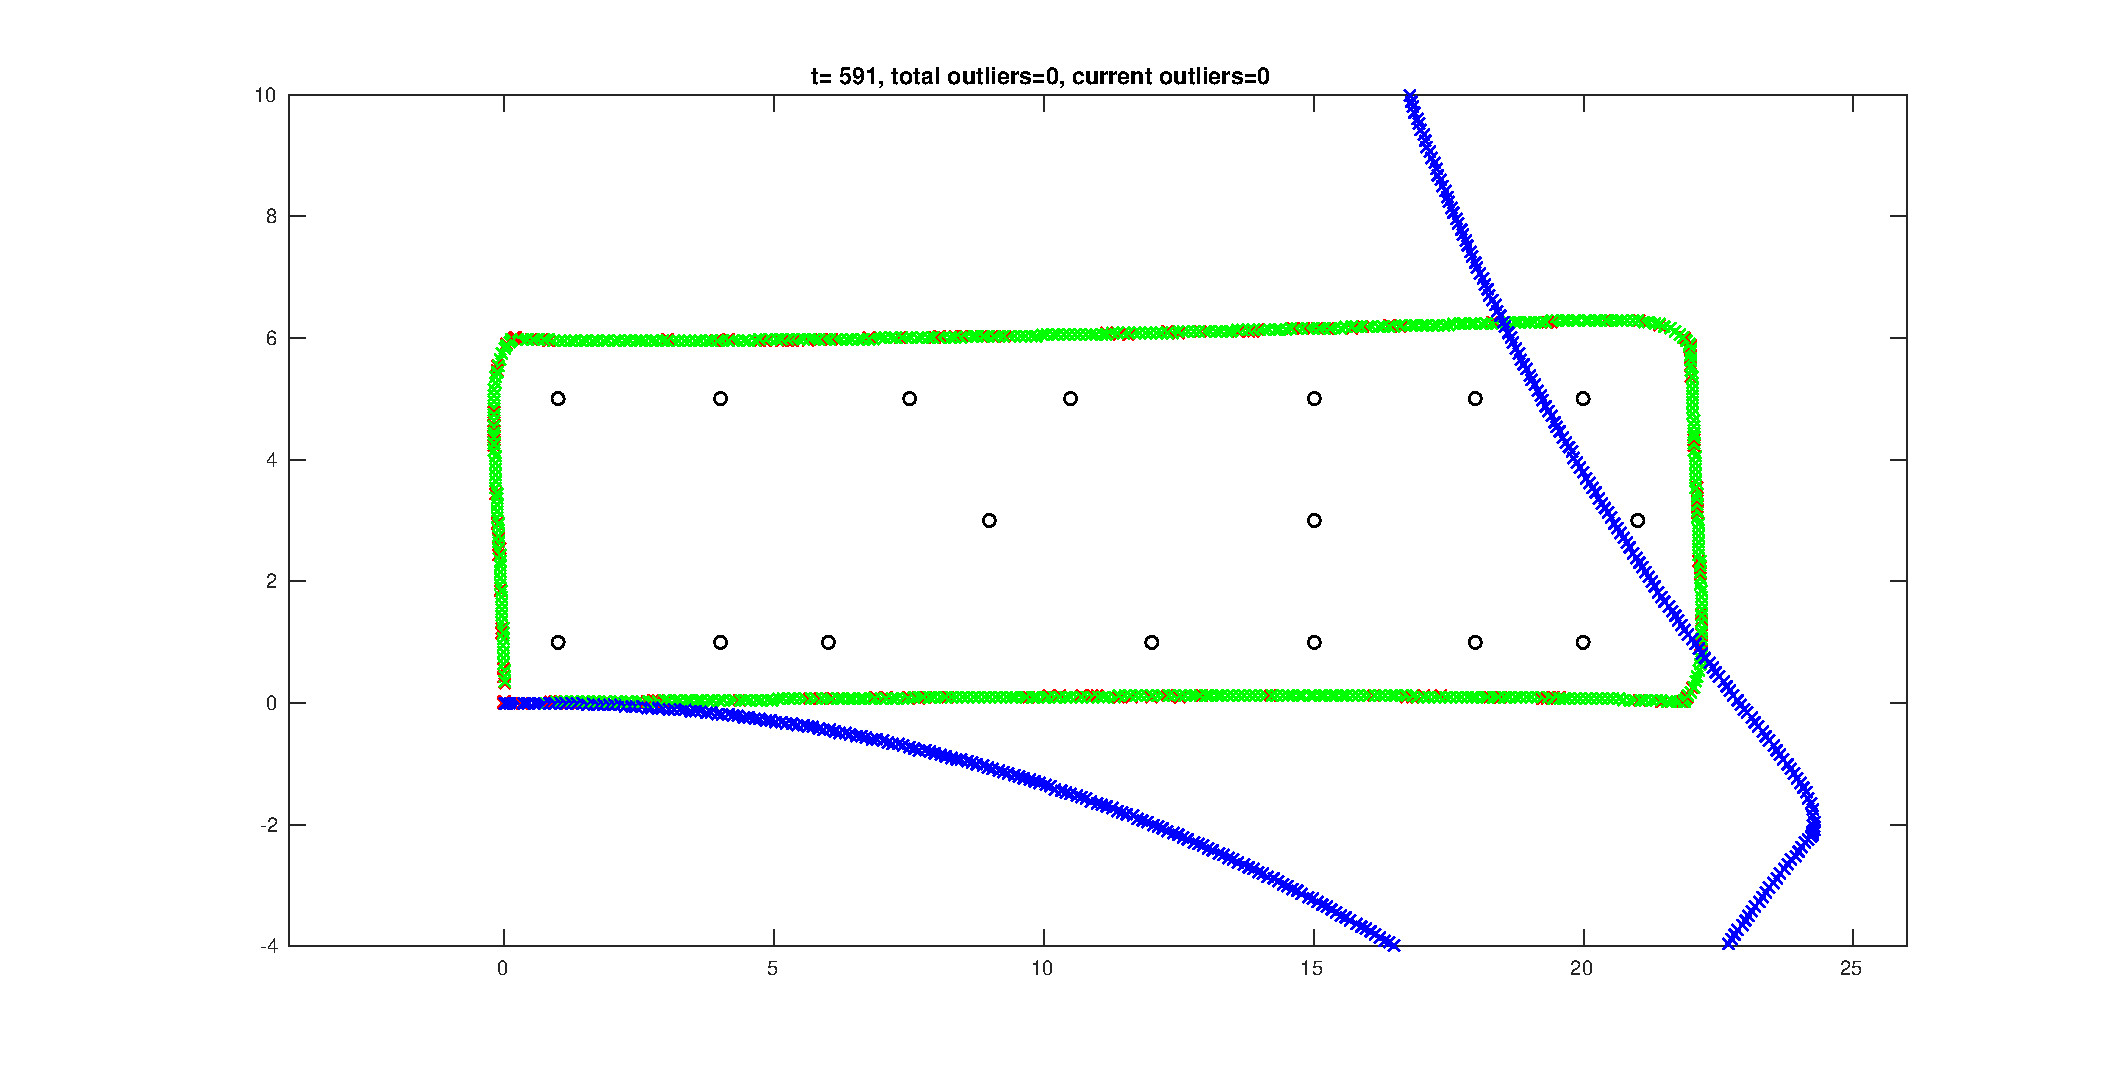
\includegraphics{./figures/part_iii_3/b1.eps}}}
	\caption{Output of the EKF for this experiment.}
	\label{fig:iii3_1}
\end{figure}

Matlab's output for the experiment using batch update was:

\textbf{mean error(x, y, theta)}=(0.000229, 0.000207, 0.000496)

\textbf{mean absolute error}=(0.003182, 0.003925, 0.002560)

\textbf{total time} = 54.454386



\subsubsection{map\_pent\_big\_10.txt + so\_pb\_10\_outlier.txt}

In this experiment the covariance matrices for the process $R$ and measurement noise $Q$ were set to:

\[
R =
\begin{bmatrix}
    0.01^2  & 0			& 0 \\
    0       & 0.01^2 	& 0 \\
    0       & 0 		& (\frac{2\pi}{360})^2 \\

\end{bmatrix}
\]


\[
Q =
\begin{bmatrix}
    0.2^2  & 0 \\
    0      & 0.2^2 \\

\end{bmatrix}
\]


Figure \ref{fig:iii3_2} shows the output of the EKF for this experiment.

\begin{figure}[H]
	\scalebox{0.6}{% This file was created by matlab2tikz.
%
%The latest updates can be retrieved from
%  http://www.mathworks.com/matlabcentral/fileexchange/22022-matlab2tikz-matlab2tikz
%where you can also make suggestions and rate matlab2tikz.
%
\definecolor{mycolor1}{rgb}{0.00000,0.44700,0.74100}%
%
\begin{tikzpicture}

\begin{axis}[%
width=4.521in,
height=0.849in,
at={(0.758in,4.103in)},
scale only axis,
xmin=0,
xmax=1200,
ymin=-0.5,
ymax=0.5,
axis background/.style={fill=white},
title style={font=\bfseries},
title={error on x, mean error=0.007163, mean absolute err=0.042018}
]
\addplot [color=mycolor1,solid,forget plot]
  table[row sep=crcr]{%
1	-0.000639800769761382\\
2	-0.00272691980903016\\
3	-0.00271450803326723\\
4	-0.0066348931718541\\
5	-0.00256417706511653\\
6	-0.00259199234468899\\
7	-0.00285343639062763\\
8	0.00221362610921731\\
9	0.0140054952263875\\
10	0.0163506675889432\\
11	0.012083080875521\\
12	0.0131139977406969\\
13	0.0229675241473592\\
14	0.0175343233516822\\
15	0.00960935508016724\\
16	0.0025801732040431\\
17	0.00167878389642164\\
18	0.00185244713552895\\
19	-0.00669006413953944\\
20	-0.000404559456645959\\
21	0.0134114515442705\\
22	0.0117905217389315\\
23	0.0220022756337103\\
24	0.0328018158266658\\
25	0.0248303229339175\\
26	0.022064160794365\\
27	0.0247314604925155\\
28	0.0293983023593504\\
29	0.0187977305979236\\
30	0.0176537785618834\\
31	0.0130276545834299\\
32	0.00802392296492351\\
33	0.0187077291756682\\
34	0.0186579811835493\\
35	0.0207596590109785\\
36	0.0368850163690642\\
37	0.0208295966298372\\
38	0.0110447432675038\\
39	0.00339047091393413\\
40	0.0137738758838837\\
41	0.0117210571789143\\
42	0.0185070813358231\\
43	0.0207865580519055\\
44	0.0142722141048459\\
45	0.0157915273307243\\
46	0.0239905445696439\\
47	0.0313082270542213\\
48	0.0387793846440971\\
49	0.0412532011625106\\
50	0.0392291492743113\\
51	0.0379908650192131\\
52	0.0304432315716223\\
53	0.0331741132380259\\
54	0.0279206615286016\\
55	0.0550659986427047\\
56	0.0326700492198078\\
57	0.0376774484574134\\
58	0.0309986001397651\\
59	0.0221696500717883\\
60	0.0245973264013943\\
61	0.0136553455107056\\
62	0.0264080766235784\\
63	0.0127805349445618\\
64	0.0184022646326261\\
65	0.0177836047283011\\
66	0.0496558547410229\\
67	0.0501451375921902\\
68	0.0235922538954543\\
69	0.0167714061811122\\
70	0.0253673969045634\\
71	0.0231343703953968\\
72	0.0107957893849193\\
73	0.00819216132597744\\
74	0.000312075955197555\\
75	-0.00496174368343016\\
76	-0.0132860278826035\\
77	-0.014254454326176\\
78	0.0132397064301133\\
79	0.00575887959147359\\
80	-0.0105403467342733\\
81	-0.00850432448598692\\
82	-0.00292732871787293\\
83	-0.00534220388845008\\
84	-0.0139091385858033\\
85	-0.0117807099113399\\
86	-0.0173193180494582\\
87	-0.0162192797164737\\
88	-0.0212130908306614\\
89	-0.0244259424243383\\
90	-0.0296676311690662\\
91	-0.0408771718017087\\
92	-0.0565112483859476\\
93	-0.0357654610217255\\
94	-0.0505251081375806\\
95	-0.0560896539661518\\
96	-0.0575769427265993\\
97	-0.0491574887864502\\
98	-0.0510559633665905\\
99	-0.0451394158105315\\
100	-0.0502430444422727\\
101	-0.0513945090507545\\
102	-0.0484003824363484\\
103	-0.0379996780893386\\
104	-0.049120111781185\\
105	-0.0258807359927946\\
106	-0.0356112733188387\\
107	-0.0384689055455638\\
108	-0.00970391891067068\\
109	-0.0179995257059293\\
110	-0.021651336807134\\
111	-0.0233551625878423\\
112	-0.0199128267072839\\
113	-0.0132771502328568\\
114	-0.0178851190700344\\
115	-0.0154219924876342\\
116	-0.0113245211148767\\
117	-0.00783137435874881\\
118	-0.00868560107529337\\
119	-0.00141294965296579\\
120	-0.00903550065556935\\
121	-0.037250190729996\\
122	-0.0339640314904872\\
123	-0.0502817642530085\\
124	-0.0735277689008207\\
125	-0.0836588938393237\\
126	-0.0982535342922279\\
127	-0.0849528018376953\\
128	-0.0765724228780629\\
129	-0.0777857780669104\\
130	-0.0593305286248773\\
131	-0.0564198614243936\\
132	-0.0700337763881191\\
133	-0.0704434906305211\\
134	-0.0906247988036695\\
135	-0.0927788182546512\\
136	-0.0949811586911902\\
137	-0.0875985686146241\\
138	-0.0710670632805179\\
139	-0.0696431056697442\\
140	-0.0584309963409284\\
141	-0.0597571916044162\\
142	-0.0698118786093289\\
143	-0.0766808243838355\\
144	-0.0777387644528407\\
145	-0.0849381622043897\\
146	-0.0777716784828621\\
147	-0.0946491381181893\\
148	-0.0885872072139247\\
149	-0.08734431663565\\
150	-0.102732624468943\\
151	-0.10106960269411\\
152	-0.107997754117148\\
153	-0.099765427553006\\
154	-0.0864906524503599\\
155	-0.0604115950947239\\
156	-0.0479635680546524\\
157	-0.0596757639699907\\
158	-0.0370761308116103\\
159	-0.0403435216917654\\
160	-0.0379508282520336\\
161	-0.0315252645856825\\
162	-0.0326519214272523\\
163	-0.0385370977415311\\
164	-0.0376839696275653\\
165	-0.0216484364654956\\
166	-0.00913568465076064\\
167	-0.00811683405301178\\
168	0.00435748244692391\\
169	-0.000690340201328965\\
170	-0.00117418563503691\\
171	-0.0327932029604128\\
172	-0.0340638565380189\\
173	-0.0366130045303921\\
174	-0.0139091349668092\\
175	-0.00422544864761054\\
176	0.00149343171489669\\
177	-0.020169039179871\\
178	-0.034514029375039\\
179	-0.012486476410956\\
180	0.0191813623962052\\
181	0.0201943280761547\\
182	0.0203813745177097\\
183	0.0242494453067454\\
184	0.0268333984440989\\
185	0.0223609953419643\\
186	-0.00165344769292375\\
187	0.00157587068453502\\
188	-0.0114914232380006\\
189	-0.00607943011430834\\
190	-0.0151290154030672\\
191	-0.0246393656236847\\
192	-0.0048536800255512\\
193	-0.0105616069587242\\
194	-0.00940692995685666\\
195	0.00366403009126337\\
196	-0.00221245308341445\\
197	-0.00660917094669422\\
198	-0.0241303464558005\\
199	-0.0178732236440773\\
200	-0.0217734769618243\\
201	-0.0144494893051306\\
202	-0.00169163825597174\\
203	-0.027856067033504\\
204	-0.0224093451765839\\
205	-0.0202544194219243\\
206	-0.0185429146153524\\
207	-0.0114024034300968\\
208	-0.00486929491804844\\
209	-0.0120205150347505\\
210	0.0164821080256381\\
211	0.00746839010202649\\
212	0.00476534935284612\\
213	0.00718577415677757\\
214	0.00479966962197587\\
215	-0.00582335053946714\\
216	-0.00954974091006733\\
217	0.00248049570134334\\
218	0.00473721718556774\\
219	0.0132414559914498\\
220	0.0151348469653012\\
221	0.0224313706938357\\
222	0.0293189111936467\\
223	0.0491851766037801\\
224	0.0607401034918933\\
225	0.0719155508035314\\
226	0.0671810430119866\\
227	0.0672479757658841\\
228	0.0569987469098141\\
229	0.0444942603875749\\
230	0.0323335806574487\\
231	0.00768800797562008\\
232	0.00572698677299677\\
233	0.00616102671391161\\
234	0.0140733626641527\\
235	0.0290598126272386\\
236	0.0285953969476882\\
237	0.0315408801079453\\
238	0.0389989079738307\\
239	0.0264371130746142\\
240	0.0152404208218204\\
241	0.0119056128507982\\
242	0.0105694945714241\\
243	0.0130859754843584\\
244	0.00905118323680831\\
245	0.00309273367626517\\
246	0.021434178811548\\
247	0.00925943020562592\\
248	0.0175473089333344\\
249	0.011609945608555\\
250	0.0195077967554909\\
251	0.00519175304441077\\
252	0.00808442216426286\\
253	0.0121698232661736\\
254	0.0220416445984295\\
255	0.0142216171063048\\
256	0.00659465793364156\\
257	0.00375544375370573\\
258	0.00113240706327211\\
259	0.00434622528249129\\
260	0.0088658631941545\\
261	0.00781232545257637\\
262	0.0126287302744821\\
263	0.00717568885823994\\
264	0.00743539767868384\\
265	0.0109842601386987\\
266	0.00872185677058113\\
267	0.00397418590240761\\
268	0.000316189054416327\\
269	-0.00438763779558471\\
270	-0.000246663423467908\\
271	0.00132012432820616\\
272	-0.00257466894588632\\
273	-0.00126533124326755\\
274	0.00221738123206805\\
275	0.00102585046697001\\
276	0.00390144486101818\\
277	0.00933735075799191\\
278	0.00529526238068456\\
279	0.012266819016638\\
280	0.0166965461344724\\
281	0.0176853338691316\\
282	0.0203228867412193\\
283	0.0236000753415055\\
284	0.0256866967361269\\
285	0.0278617130575043\\
286	0.0371876253398575\\
287	0.0366532208967705\\
288	0.0349876502858173\\
289	0.0260967290411145\\
290	0.00139917254479371\\
291	-0.00322957051008288\\
292	0.00471343631561894\\
293	-0.000816962468899618\\
294	0.000718247973189534\\
295	-0.0114253792275534\\
296	0.00240798317529922\\
297	0.00835843114355583\\
298	0.00735066435719745\\
299	0.000817373873243099\\
300	-0.0167136533956587\\
301	-0.000599486344018629\\
302	-0.0197422111224341\\
303	0.00381594519533479\\
304	-0.0186545657542112\\
305	0.00779948051802748\\
306	-0.0118548449488038\\
307	-0.00142191645535306\\
308	-0.00976157131435684\\
309	-0.0189147989690959\\
310	-0.00548809921826177\\
311	-0.0055356578035024\\
312	-0.0069378242643019\\
313	0.00401771764891024\\
314	0.0101330912079298\\
315	0.0230852676309752\\
316	0.0194276930976223\\
317	0.0295524027985472\\
318	0.000368502243919266\\
319	-0.0122939561312734\\
320	-0.026128438842953\\
321	-0.0414608031613888\\
322	-0.0714131235156579\\
323	-0.0698621927031837\\
324	-0.0646445204613606\\
325	-0.0649722296948916\\
326	-0.0649668876490033\\
327	-0.0673120161271825\\
328	-0.0631871653770979\\
329	-0.0515518256034824\\
330	-0.0326074744908418\\
331	-0.0291652923016699\\
332	-0.0389998350745415\\
333	-0.049183746240228\\
334	-0.061341337148221\\
335	-0.0467704095498576\\
336	-0.0490672060033859\\
337	-0.0586355562387233\\
338	-0.060214986018913\\
339	-0.0450892051731415\\
340	-0.0363021787670199\\
341	-0.0242099646064489\\
342	-0.0313856547013565\\
343	-0.0502769723936431\\
344	-0.057751798956037\\
345	-0.056019960323944\\
346	-0.0603157185383516\\
347	-0.0430773834112692\\
348	-0.0299436269923028\\
349	-0.0295132037150516\\
350	-0.0333172297211703\\
351	-0.050114389468515\\
352	-0.0471423587255799\\
353	-0.0410850259357893\\
354	-0.0236834674238935\\
355	-0.0176481419004553\\
356	-0.00489275644136811\\
357	0.028880361648973\\
358	0.0222744405761546\\
359	0.0051961849902824\\
360	0.0462662456203766\\
361	0.031351044982376\\
362	0.0427025248556809\\
363	0.0538124417456594\\
364	0.0522560696070862\\
365	0.0603009377950485\\
366	0.0688668624348878\\
367	0.0685505802470736\\
368	0.0804622682528446\\
369	0.105751537255674\\
370	0.131218534973438\\
371	0.132928562158742\\
372	0.151219043438108\\
373	0.190636449062694\\
374	0.219452184303965\\
375	0.202375089833151\\
376	0.195256945566886\\
377	0.160022696336121\\
378	0.177175687002439\\
379	0.15653012613754\\
380	0.158515075796842\\
381	0.152344645582712\\
382	0.14651042843937\\
383	0.13623769556834\\
384	0.126839177282456\\
385	0.118764795519144\\
386	0.105844062548432\\
387	0.106043693321574\\
388	0.124449816865091\\
389	0.151563401660344\\
390	0.153103404212931\\
391	0.171050369954369\\
392	0.143798593102353\\
393	0.130403739288656\\
394	0.122805765350872\\
395	0.126572263847109\\
396	0.121821971459795\\
397	0.123717389687322\\
398	0.099971243347845\\
399	0.0750402577872258\\
400	0.032318754820583\\
401	0.053974738448904\\
402	-0.0274256152836401\\
403	-0.0712643992077844\\
404	-0.0452516640073277\\
405	-0.0193920606602305\\
406	-0.0022391833430575\\
407	0.0403294092115303\\
408	-0.0206959153738957\\
409	0.0167924911580428\\
410	-0.0126693480935991\\
411	-0.00954208899573317\\
412	-0.0510364999037876\\
413	-0.0494501640393743\\
414	-0.0217924724608629\\
415	-0.0200861112346793\\
416	0.000648092047359938\\
417	0.0327774805297096\\
418	0.0332570883576153\\
419	0.0516206117485503\\
420	0.0596379329477585\\
421	0.06424696671532\\
422	0.0463349760231679\\
423	0.0249593606720602\\
424	0.0162222674902317\\
425	-0.00787225964252869\\
426	-0.00825334787592524\\
427	-0.00932917724814786\\
428	0.0241910281887279\\
429	-0.0152752184380631\\
430	-0.0127540408561586\\
431	-0.00762825685580637\\
432	0.00099189112988185\\
433	0.0143424179894147\\
434	0.0231900406964805\\
435	0.0383633734094317\\
436	0.0228460552157976\\
437	0.0300247968467708\\
438	0.0278382938618833\\
439	0.0176632569797199\\
440	0.0177225549286213\\
441	0.0137339374275776\\
442	0.00735165454216968\\
443	0.037063543688344\\
444	0.0162159265352066\\
445	0.00878932184642167\\
446	0.0246787638335064\\
447	0.0228573703882908\\
448	0.0356615681708838\\
449	0.0216749606836046\\
450	0.027738913618748\\
451	0.0197388107916616\\
452	0.00880032638315598\\
453	0.00684906075829872\\
454	0.0293617408824325\\
455	0.0418874095195036\\
456	0.0274907808528297\\
457	0.0372697922006573\\
458	0.0633666393126155\\
459	0.0728397249439219\\
460	0.0586794586692712\\
461	0.0556886829157719\\
462	0.0630406202596063\\
463	0.0625023358445382\\
464	0.0534170199648756\\
465	0.0264587138568189\\
466	0.0113092756611763\\
467	0.019138716404246\\
468	0.0266168008400562\\
469	0.00861954783680119\\
470	-0.0160233782559551\\
471	-0.0010665687907121\\
472	-0.0194603366934167\\
473	-0.0296227822581692\\
474	-0.0214749375536059\\
475	-0.0119906154760372\\
476	-0.00432028026867926\\
477	0.000165961183014929\\
478	0.0238782802495585\\
479	-0.014874795544106\\
480	0.0192602173524818\\
481	-0.0125932667501942\\
482	-0.0160169603784759\\
483	-0.00877678578001451\\
484	0.00314249048185644\\
485	-0.0102952191986958\\
486	-0.0244352016714871\\
487	-0.0197421928874419\\
488	-0.0168363911078835\\
489	-0.0394596979068567\\
490	-0.0611975466686516\\
491	-0.0800575947245541\\
492	-0.0785859050091773\\
493	-0.083240398875521\\
494	-0.0858890785225803\\
495	-0.103579317230533\\
496	-0.128837734329345\\
497	-0.130051345395774\\
498	-0.110012668972757\\
499	-0.0990549831237395\\
500	-0.112673732656575\\
501	-0.113264511922438\\
502	-0.0873586900730778\\
503	-0.0780834421502519\\
504	-0.0527509002530948\\
505	-0.0498269777711791\\
506	-0.0471450382899086\\
507	-0.0421847686197943\\
508	-0.0449263040193593\\
509	-0.0246766132128009\\
510	-0.0115770977894307\\
511	-0.0406130523178803\\
512	-0.0333408355933642\\
513	-0.0541733634292427\\
514	-0.0790552840409049\\
515	-0.0511765562990618\\
516	-0.0686881082606732\\
517	-0.0685055204568243\\
518	-0.0956895982110808\\
519	-0.0827430973321697\\
520	-0.0535681809238255\\
521	-0.0448996199744514\\
522	-0.0401793829348271\\
523	-0.0562284818347898\\
524	-0.0223758599513033\\
525	-0.0153486566972418\\
526	-0.018074894273127\\
527	-0.0167007845933647\\
528	-0.0135040158294863\\
529	0.0107739564533524\\
530	0.0279429570213487\\
531	-0.00108162966990122\\
532	-0.0135523576613004\\
533	-0.013394429374447\\
534	0.00230350262305379\\
535	-0.0107113692286234\\
536	0.0137321886569559\\
537	-0.0031248357284781\\
538	-0.0100031367559588\\
539	-0.0113317804521849\\
540	-0.0130851697757457\\
541	0.00163505921125662\\
542	-0.00348325396445404\\
543	-0.0178478884086033\\
544	0.0157062867977338\\
545	0.0263546882857248\\
546	0.0533727777655315\\
547	0.0722271489188202\\
548	0.0697562080816283\\
549	0.0530910616496527\\
550	0.0592749314042393\\
551	0.0521933214350376\\
552	0.0918204883815612\\
553	0.0770757507855855\\
554	0.0433210836239404\\
555	0.05894160555426\\
556	0.0299803172267694\\
557	0.0450644434318797\\
558	0.00960197567447096\\
559	0.0283690266920225\\
560	0.00691491451406279\\
561	0.0246295301879087\\
562	0.00461491294164773\\
563	-0.0220955202420221\\
564	0.00318578479295084\\
565	-0.00779815059004463\\
566	0.0116466154425332\\
567	0.0178147272730769\\
568	0.0203365234249269\\
569	0.0290131921841876\\
570	-0.0127238017044498\\
571	-0.0116297829389289\\
572	0.00323416489957395\\
573	0.0199450061369255\\
574	0.0392415030619588\\
575	0.0267351709054857\\
576	0.0484401358701518\\
577	-0.00266776543942626\\
578	-0.0225703393471086\\
579	-0.0358067730778444\\
580	-0.0135464291798328\\
581	0.0036771946607459\\
582	-0.0252109506961951\\
583	0.0119670544860284\\
584	0.0397766140963469\\
585	0.0412844181468728\\
586	0.014557302554028\\
587	-0.0173515454692001\\
588	-0.0206322653960029\\
589	-0.050866041457521\\
590	-0.0318619681326098\\
591	-0.0415159938910286\\
592	-0.0376047289527186\\
593	-0.0448117737158498\\
594	-0.0612443961103004\\
595	-0.0630650105718793\\
596	-0.0765364562147184\\
597	-0.0951900367541363\\
598	-0.114781836323793\\
599	-0.101551061254202\\
600	-0.0951271940526901\\
601	-0.113368738694479\\
602	-0.112129774769151\\
603	-0.126228983792515\\
604	-0.104612327037085\\
605	-0.111941357321772\\
606	-0.113918818490202\\
607	-0.137724969310046\\
608	-0.128438519966458\\
609	-0.113204017806886\\
610	-0.108391092553088\\
611	-0.103709066733764\\
612	-0.0858138596136833\\
613	-0.0420220446449946\\
614	-0.0711978684660757\\
615	-0.0262703292222959\\
616	-0.0589125667156694\\
617	-0.0749760101393768\\
618	-0.0690670869969985\\
619	-0.0638554086744314\\
620	-0.0781601536905363\\
621	-0.0704086866605493\\
622	-0.0727797531077705\\
623	-0.0608257876181568\\
624	-0.0629438537975453\\
625	-0.0597411468956359\\
626	-0.055219790229895\\
627	-0.0578831262754456\\
628	-0.0631675372217479\\
629	-0.0618035914190642\\
630	-0.0692545931521913\\
631	-0.0740785580738503\\
632	-0.0629327574475127\\
633	-0.0554489439384476\\
634	-0.0490602217361555\\
635	-0.0579978720371273\\
636	-0.0503442365829088\\
637	-0.0496656012922756\\
638	-0.0438857359553495\\
639	-0.0549451426034722\\
640	-0.0674624571156777\\
641	-0.0500718723351099\\
642	-0.0767879670213034\\
643	-0.0654122011927711\\
644	-0.0770701755747325\\
645	-0.0671334118806186\\
646	-0.0891194130178441\\
647	-0.0695076182023904\\
648	-0.0864908492900298\\
649	-0.0735881482581249\\
650	-0.0698990693223251\\
651	-0.0504337156212564\\
652	-0.0386408922116956\\
653	-0.0353431436368297\\
654	-0.0321440923141658\\
655	-0.0112337572926933\\
656	-0.0165648384471027\\
657	-0.0175290697276118\\
658	0.0106885046921974\\
659	0.00430194958175178\\
660	0.00303172474304958\\
661	-0.0154772306574706\\
662	-0.00732038002469793\\
663	-0.0155933596096318\\
664	-0.0475518601968297\\
665	-0.0655319679894149\\
666	-0.0570986235604671\\
667	-0.0234676566227741\\
668	-0.0171802852996876\\
669	-0.0166067284671847\\
670	-0.0173393117741689\\
671	-0.0191717823273834\\
672	-0.00973811186099738\\
673	-0.00800248332818754\\
674	-0.0281193923658662\\
675	-0.0400228817408674\\
676	-0.0122859316155655\\
677	-0.00604735396789025\\
678	-0.0113428847428878\\
679	-0.00257337154556936\\
680	-0.00674062976577616\\
681	0.00223336700506138\\
682	-0.0102851489698068\\
683	0.00117884772413746\\
684	-0.00516345681473851\\
685	0.0211063464244745\\
686	0.0145751763928459\\
687	0.00345883358468058\\
688	0.00398034601582964\\
689	0.0183051410435802\\
690	0.0194150369483275\\
691	-0.00953553500058746\\
692	0.00212469873226695\\
693	-0.00126425696671717\\
694	0.0114133875202782\\
695	0.0177451937212076\\
696	0.028805018413955\\
697	0.0264145145763948\\
698	0.0293643838673283\\
699	0.0270581873436591\\
700	0.037037561831859\\
701	0.0396829684627775\\
702	0.0443540105392266\\
703	0.0351644626289627\\
704	0.0358954331645549\\
705	0.034583347261826\\
706	0.0567121704312576\\
707	0.0742034954359703\\
708	0.0719792380510214\\
709	0.0729968291496235\\
710	0.0674760054507892\\
711	0.0640836524471915\\
712	0.0661970274454724\\
713	0.0638953555493273\\
714	0.0547335027474105\\
715	0.0454914593021307\\
716	0.0476532362516835\\
717	0.0373508702297585\\
718	0.0262798813856726\\
719	0.0369157934612581\\
720	0.0604788259939468\\
721	0.0602974476751825\\
722	0.058584843751138\\
723	0.0524602127276879\\
724	0.0376043188108959\\
725	0.0470527399764791\\
726	0.0322182386987624\\
727	0.0453488752464661\\
728	0.0436016366652012\\
729	0.0497755361773304\\
730	0.0636661022669802\\
731	0.061130130348932\\
732	0.0739736716324533\\
733	0.082387697150244\\
734	0.0778611582853266\\
735	0.0748138132446865\\
736	0.0701110240395746\\
737	0.0785253900367007\\
738	0.0629894970420057\\
739	0.0624270768722432\\
740	0.0432914222202161\\
741	0.0359297663903497\\
742	0.0204157135991192\\
743	0.0280729385360043\\
744	0.033646861404339\\
745	0.0385794177127892\\
746	0.0241250722214108\\
747	0.0122738064696115\\
748	0.000466025076319099\\
749	-0.000725274457060721\\
750	0.00113032819363212\\
751	-0.00453106005570092\\
752	-0.0151212516125057\\
753	-0.00608249664086635\\
754	-0.00547727828259781\\
755	-0.0178032325751722\\
756	-0.0172150290439586\\
757	-0.0225101767894333\\
758	-0.0267044989092415\\
759	-0.0105133677195237\\
760	0.000375448823749736\\
761	-0.00325316503194095\\
762	-0.00448230921306525\\
763	-0.00612228017551786\\
764	0.00734899565736669\\
765	0.0118993423216249\\
766	0.0245369251228134\\
767	0.0253380292829455\\
768	0.0139959132071041\\
769	0.0130263067377392\\
770	0.00741819082572981\\
771	-0.00844266146429007\\
772	-0.0318769477203045\\
773	-0.0422239206273964\\
774	-0.0465871665068569\\
775	-0.0431080961181944\\
776	-0.0394461797212156\\
777	-0.0387000298404061\\
778	-0.0413028185901574\\
779	-0.0444554684335845\\
780	-0.0263531268504842\\
781	-0.010562938551141\\
782	0.00417902377955137\\
783	0.018587659898273\\
784	0.0235257912021201\\
785	0.0114015472443647\\
786	0.00830463597301367\\
787	0.00766125341295698\\
788	0.00677822229923741\\
789	0.00645520403198319\\
790	0.0154825999974744\\
791	0.00360154126928514\\
792	-0.00521598732865236\\
793	0.00396380031635779\\
794	-0.00695775044307467\\
795	-0.00988965890505078\\
796	-0.0353504219007768\\
797	-0.0400906872333753\\
798	-0.0367425993256845\\
799	-0.0209252260385444\\
800	-0.0156769776938486\\
801	0.000665952439526052\\
802	0.00186026342821322\\
803	-0.0065425827733705\\
804	-0.0113028901009216\\
805	-0.00204533629830461\\
806	-0.00400252479341301\\
807	0.00305319157570594\\
808	0.00882751378747226\\
809	0.0123458469063573\\
810	0.00776434245715318\\
811	0.0072874391101454\\
812	0.0122512905902514\\
813	0.0222985838686238\\
814	0.0211262199762121\\
815	0.017628196659353\\
816	0.0318036064032095\\
817	0.0334846717023565\\
818	0.0318456487507266\\
819	0.0261413836922157\\
820	0.0208677378083069\\
821	0.0132125635917131\\
822	0.0120010570098374\\
823	0.00703104708960645\\
824	0.00857024527291816\\
825	0.0158572970209931\\
826	0.0026122289004622\\
827	0.00459739255409986\\
828	0.0113430638631984\\
829	0.0151142941459117\\
830	0.0104409562274883\\
831	0.0107577178668468\\
832	0.0130214122259087\\
833	0.0105085721085292\\
834	0.00817993992029997\\
835	0.00198627226059855\\
836	0.00564570987418023\\
837	0.00580721479073176\\
838	0.00481536953942996\\
839	0.00553211263648645\\
840	0.00619020290889427\\
841	0.0119070571926096\\
842	0.0153224924710562\\
843	0.0165920166856592\\
844	0.019258621602666\\
845	0.0184517822760526\\
846	0.0232718240239858\\
847	0.0182910450667406\\
848	0.0246127620583114\\
849	0.0218632483169237\\
850	0.0220611078750204\\
851	-0.00240471616883475\\
852	0.0178042665357574\\
853	0.0383222531884369\\
854	0.00239304546438923\\
855	-0.0101166592502451\\
856	-0.00355671042618466\\
857	0.0206881660677425\\
858	0.0379846750371082\\
859	0.056062647996046\\
860	0.0340944746230343\\
861	0.0612525641602617\\
862	0.059066347432398\\
863	0.0418954578525246\\
864	0.0308276836939507\\
865	0.0353328100568344\\
866	0.0233375349312523\\
867	0.0133994745581805\\
868	0.0216780595627066\\
869	0.00745652240609918\\
870	0.00714280414179225\\
871	0.00277141879340848\\
872	0.0152048108114842\\
873	-0.00479228350317351\\
874	-0.0107251723602571\\
875	-0.00835135988608915\\
876	-0.0184113045848682\\
877	-0.0219132665080219\\
878	0.00401143168516738\\
879	-0.00385572269105117\\
880	0.0129729538714609\\
881	0.00322437540909237\\
882	0.0210593232433556\\
883	0.0371026280274124\\
884	0.0459209844542097\\
885	0.0827652515823466\\
886	0.0641411198647426\\
887	0.0591083242450198\\
888	0.0797889019135215\\
889	0.0833828614311851\\
890	0.0869022339734448\\
891	0.0727364231009711\\
892	0.0677727415363312\\
893	0.0754440116324029\\
894	0.0549827907273221\\
895	0.0506692686504646\\
896	0.0752555739260383\\
897	0.0675948448334048\\
898	0.0506648921119582\\
899	0.0496497876019351\\
900	0.0503275349483103\\
901	0.0621641139009925\\
902	0.0568967546498148\\
903	0.0603241028175628\\
904	0.0499476339650751\\
905	0.0293250465818087\\
906	0.0351668018142475\\
907	0.033287017152861\\
908	0.0241227405779267\\
909	0.0202474319272674\\
910	0.0154944418030558\\
911	0.0375024067928915\\
912	0.0664828029454259\\
913	0.0416294767565513\\
914	0.0521937971958892\\
915	0.0748282836898635\\
916	0.0568643867337491\\
917	0.0419508865444003\\
918	0.0532131987743152\\
919	0.0549452593985045\\
920	0.0733632514356684\\
921	0.0662592136339155\\
922	0.0539568883407657\\
923	0.0370135132335063\\
924	0.0323002831385342\\
925	0.0250528974809154\\
926	0.0081841742729023\\
927	0.00565326591650894\\
928	0.0023435772369802\\
929	0.00196673187045304\\
930	0.0192208158807237\\
931	0.0148369007889633\\
932	0.017932801246324\\
933	0.0101154949664415\\
934	0.0022888210117995\\
935	0.00764754800343903\\
936	-0.0301220477830011\\
937	-0.00110491101703758\\
938	-0.00250037794161662\\
939	0.0234363241662021\\
940	0.042639758745568\\
941	0.0346232817972161\\
942	0.0432149309075598\\
943	0.0441782559795714\\
944	0.0425705452576706\\
945	0.0364548961752438\\
946	0.0266326685226783\\
947	0.0265287141221102\\
948	0.0457004188771895\\
949	0.0480665840075671\\
950	0.0646538116021578\\
951	0.0620442337986367\\
952	0.0586759591525476\\
953	0.0671807558496615\\
954	0.0693825498563143\\
955	0.0657866460087693\\
956	0.0894237233750275\\
957	0.0921939731549539\\
958	0.0908531095472442\\
959	0.0718069691557535\\
960	0.0806338880933914\\
961	0.0905697130228562\\
962	0.0851970745737649\\
963	0.10727292807093\\
964	0.143691861654689\\
965	0.116883959599106\\
966	0.0893648270951601\\
967	0.0837247137588957\\
968	0.0413002855054438\\
969	0.0420581628051941\\
970	0.0241674480099006\\
971	0.0450667104220583\\
972	0.0433260733431275\\
973	0.0185182043305412\\
974	0.0358758031652409\\
975	0.0588050558334956\\
976	0.0321148561558182\\
977	0.03867074697897\\
978	0.0512410418270157\\
979	0.0124042159214435\\
980	-0.00403883804409588\\
981	-0.000330810496554257\\
982	0.0373485827875957\\
983	0.032089158497814\\
984	0.0228670134150795\\
985	-0.00483695036388276\\
986	-0.00323901068922972\\
987	0.0119705617291066\\
988	0.0299149506456766\\
989	0.0280341479785111\\
990	0.0306385815114192\\
991	-0.00974126166014244\\
992	0.00414230153765782\\
993	-0.0303850934799685\\
994	-0.038698944030247\\
995	-0.0132530602080791\\
996	-0.00879350786526256\\
997	0.0130271524812215\\
998	0.00548538720033243\\
999	0.0174509560468419\\
1000	0.0184244989313012\\
1001	0.00519989701900592\\
1002	-0.00341673228477113\\
1003	0.0175280055665255\\
1004	0.0513840885004582\\
1005	0.0575874951111688\\
1006	0.0829994884482268\\
1007	0.115019682029302\\
1008	0.0567855015375169\\
1009	0.0686444729133413\\
1010	0.0644950669320679\\
1011	0.084633490101794\\
1012	0.0709822324278875\\
1013	0.0771717426668834\\
1014	0.0788913718883144\\
1015	0.0966613330319062\\
1016	0.112642951054999\\
1017	0.15626842771125\\
1018	0.145629017501598\\
1019	0.127406305175955\\
1020	0.128713250051027\\
1021	0.121268769512201\\
1022	0.100821769188375\\
1023	0.0833842325403609\\
1024	0.035857212951937\\
1025	0.0169328730411147\\
1026	0.0537314256088468\\
1027	0.0707137943327876\\
1028	0.0981847601776185\\
1029	0.0931974464890191\\
1030	0.0853837629716967\\
1031	0.0955208351731374\\
1032	0.098050703709446\\
1033	0.0905638938520275\\
1034	0.051056745793252\\
1035	0.0558325647419595\\
1036	0.0389902632192163\\
1037	0.0227293013197221\\
1038	-0.0137340583110577\\
1039	-0.00303434859148499\\
1040	-0.00858038805496619\\
1041	-0.013754473613651\\
1042	0.011860444133192\\
1043	-0.00353127333610459\\
1044	-0.0027910498254311\\
1045	-0.00436581937011393\\
1046	-0.0334456119897109\\
1047	-0.0253786183633649\\
1048	-0.037933084105477\\
1049	-0.0506595033383448\\
1050	-0.0389777783540222\\
1051	-0.0637951950121627\\
1052	-0.0698085007278362\\
1053	-0.107257379081238\\
1054	-0.0929771123962784\\
1055	-0.0775850411042729\\
1056	-0.0775430871819855\\
1057	-0.0847350497137391\\
1058	-0.09000110589204\\
1059	-0.0863575878276075\\
1060	-0.099449439108005\\
1061	-0.0627077958829982\\
1062	-0.0640972585630033\\
1063	-0.0817787058156911\\
1064	-0.0745883754073162\\
1065	-0.0747339259478093\\
1066	-0.10777124399222\\
1067	-0.0796455364900837\\
1068	-0.0688392573155214\\
1069	-0.0829203576021751\\
1070	-0.067223374591463\\
1071	-0.0660043330564459\\
1072	-0.0731293627416472\\
1073	-0.0824308186162606\\
1074	-0.0574283652096002\\
1075	-0.0616592567502732\\
1076	-0.0909386142809305\\
1077	-0.109759740611523\\
1078	-0.0849228927695735\\
1079	-0.0618831390077039\\
1080	0.0175750351224471\\
1081	-0.0131116942796838\\
1082	-0.0123407695156015\\
1083	0.0541300810953285\\
1084	0.0803665486177678\\
1085	0.018246004853637\\
1086	0.0568883083210263\\
1087	0.0896735770888375\\
1088	0.123124873271466\\
1089	0.122170661223006\\
1090	0.106457082482065\\
1091	0.114827756982882\\
1092	0.117912884670722\\
1093	0.115560549143411\\
1094	0.119793310845387\\
1095	0.11081867518621\\
1096	0.119412790614541\\
1097	0.105215958040125\\
1098	0.131143471134337\\
1099	0.16753829582742\\
1100	0.162176120723116\\
1101	0.144326575904772\\
1102	0.120927250662794\\
1103	0.133854211853693\\
1104	0.152725768636365\\
1105	0.116254660183719\\
1106	0.120025988862096\\
1107	0.112327389073199\\
1108	0.0972151732562772\\
1109	0.117797332152001\\
1110	0.0925456347835745\\
1111	0.0957399134049473\\
1112	0.107759787968755\\
1113	0.116515721959798\\
1114	0.125926246008301\\
1115	0.168691993154192\\
1116	0.131398174456947\\
1117	0.122325157467785\\
1118	0.111090672774968\\
1119	0.151293807026698\\
1120	0.129096196693427\\
1121	0.14786111530179\\
1122	0.130783573146074\\
1123	0.149868378923336\\
1124	0.154442320324551\\
1125	0.156105572652088\\
1126	0.146031440168859\\
1127	0.14581972050776\\
1128	0.178050882145694\\
1129	0.143205208982668\\
1130	0.159812236992198\\
1131	0.155533231934024\\
1132	0.129635667534648\\
1133	0.0939157700939974\\
1134	0.0827376384898892\\
1135	0.061728004815417\\
1136	0.0424697989728866\\
1137	0.000832905852081289\\
1138	0.0105311011603177\\
1139	-0.0184176152523916\\
1140	-0.0144702125415916\\
1141	-0.0474018620273258\\
1142	-0.0493340120831531\\
1143	-0.0728743352128669\\
1144	-0.0769901253063781\\
1145	-0.0682881670923621\\
1146	-0.0667512903551399\\
1147	-0.0317410309342856\\
1148	-0.035077216715778\\
1149	-0.0432305882028698\\
1150	-0.0231914088646068\\
1151	-0.00308686408892722\\
1152	-0.0443356207275007\\
1153	-0.0549001146707351\\
1154	-0.0568932708843075\\
1155	-0.0429913580691679\\
1156	-0.0405133694059838\\
1157	-0.0516803890733968\\
1158	-0.0442996909775788\\
1159	-0.0313585078710839\\
1160	-0.0316350998283159\\
1161	-0.0359229320043397\\
1162	-0.0163701615974841\\
1163	-0.0292522011262375\\
1164	-0.0355829185622292\\
1165	-0.033949420999531\\
1166	-0.0212393710354499\\
1167	-0.0205294345759084\\
1168	-0.0227376876368424\\
1169	-0.0414360400794673\\
1170	-0.0159885032973826\\
1171	-0.015047419903699\\
1172	-0.0156338710456589\\
1173	-0.0140760858245081\\
1174	-0.0318974824775049\\
1175	-0.0290529535896455\\
1176	-0.0396847884957832\\
1177	-0.0671352191168788\\
1178	-0.0624666387423609\\
1179	-0.0743209635013167\\
1180	-0.0564614381650448\\
1181	-0.075573551726043\\
1182	-0.0646391237268711\\
1183	-0.0376137780846468\\
1184	-0.0368553499594251\\
1185	-0.0420917218741872\\
1186	-0.0514870362064057\\
1187	-0.0133134093857552\\
1188	0.0146217173135912\\
1189	0.0181557507341013\\
1190	0.0247889417830338\\
1191	0.0214168734441662\\
1192	-0.0152020463808764\\
1193	-0.0143607703627766\\
1194	-0.0155069347514303\\
1195	-0.00144315981311305\\
};
\end{axis}

\begin{axis}[%
width=4.521in,
height=0.849in,
at={(0.758in,2.292in)},
scale only axis,
xmin=0,
xmax=1200,
ymin=-0.2,
ymax=0.2,
axis background/.style={fill=white},
title style={font=\bfseries},
title={error on y, mean error=0.004752, mean absolute err=0.042067}
]
\addplot [color=mycolor1,solid,forget plot]
  table[row sep=crcr]{%
1	0.000276065025408149\\
2	0.00103350561560361\\
3	-0.000965381700926931\\
4	0.00117809196246331\\
5	0.00141764357407842\\
6	0.00550324899568082\\
7	0.00455635564473493\\
8	0.00149753596465421\\
9	0.00205693296457018\\
10	0.00369558565365484\\
11	0.00813112317072722\\
12	0.00250842798235819\\
13	-0.0016752714355959\\
14	0.00352414160591208\\
15	0.00314768216409557\\
16	0.000835185039190079\\
17	-0.00218935768245818\\
18	0.000253885039915888\\
19	0.00133066529383827\\
20	0.00805620734244982\\
21	0.00840290566439605\\
22	0.00485355743621137\\
23	0.0225276274563474\\
24	0.0312206188924418\\
25	0.0299164820478206\\
26	0.0170768095674957\\
27	0.0158396054620354\\
28	0.0208495227754466\\
29	0.0155008567820598\\
30	0.00990096283556249\\
31	0.0200996968058101\\
32	0.0238146139407603\\
33	0.0136629315947658\\
34	0.0110143986333544\\
35	0.0133093859788831\\
36	0.0116590284515735\\
37	0.00864413665153363\\
38	0.0221299903196245\\
39	0.0190893051479251\\
40	0.0210453756677336\\
41	0.0096538032797242\\
42	0.00568473664243874\\
43	0.00790486058288353\\
44	0.0114678672434967\\
45	0.0124114735551339\\
46	-0.00772296933953709\\
47	0.00160228704904486\\
48	-0.00906241987761902\\
49	-0.0273948936440807\\
50	-0.0346414161808248\\
51	-0.0315725210255842\\
52	-0.0410533598437441\\
53	-0.0364753873486778\\
54	-0.0542460351728877\\
55	-0.069997066539877\\
56	-0.0491751612823956\\
57	-0.0428753396119743\\
58	-0.0332156861334676\\
59	-0.0272527341620648\\
60	-0.0104791960425492\\
61	0.00615206732499884\\
62	0.0112310280392753\\
63	0.0189029339917164\\
64	0.0312266389492468\\
65	0.0133412922548917\\
66	-0.00291832583994944\\
67	-0.00456992367873665\\
68	0.00333424767686696\\
69	0.0131889847864683\\
70	-0.00284351963628193\\
71	0.00490271768034622\\
72	0.0107162107535657\\
73	0.0113501933505851\\
74	0.0125318395772056\\
75	-0.0027913076305448\\
76	-0.0075373892382995\\
77	-0.0248306407893364\\
78	-0.0132626983263022\\
79	-0.0190079790265694\\
80	-0.029422978215536\\
81	-0.0251354091704177\\
82	-0.0170405199412378\\
83	-0.033995541783709\\
84	-0.0409112039204524\\
85	-0.037939965064107\\
86	-0.0467657693044132\\
87	-0.0538216530098308\\
88	-0.067632884342137\\
89	-0.0610978224021452\\
90	-0.0676269456030685\\
91	-0.0536325800785091\\
92	-0.0451923177774742\\
93	-0.0326636759322487\\
94	-0.0281414771962596\\
95	-0.0316246140745604\\
96	-0.0447028529651137\\
97	-0.0316010275871625\\
98	-0.0363454028998258\\
99	-0.0328169521228596\\
100	-0.0419178365417716\\
101	-0.028576161687242\\
102	-0.0169899354579677\\
103	0.00979756077036686\\
104	0.0125924681164875\\
105	-0.0160303714864902\\
106	-0.0102876741365234\\
107	0.00558920656414852\\
108	-0.0239093714643692\\
109	-0.00634615456925758\\
110	-0.0375648243194258\\
111	-0.0588781205527624\\
112	-0.0819763861691269\\
113	-0.0524132300307905\\
114	-0.0619113182725677\\
115	-0.0587272531617344\\
116	-0.0648613582995621\\
117	-0.0649608819467034\\
118	-0.0575434077811812\\
119	-0.0733835819039914\\
120	-0.0912987237741012\\
121	-0.120816102910238\\
122	-0.111367073337584\\
123	-0.110348769015349\\
124	-0.121953295823712\\
125	-0.0780540599873873\\
126	-0.100943787925639\\
127	-0.0799063250179302\\
128	-0.0484957618939177\\
129	-0.0125750254484966\\
130	0.0169171319995884\\
131	-0.000347447356435993\\
132	-0.00621249511457478\\
133	-0.0162552725048029\\
134	-0.034197285492743\\
135	-0.0279347062676782\\
136	-0.0503511687463014\\
137	-0.0446303634256298\\
138	-0.0233794066223743\\
139	-0.00451768614502424\\
140	-0.00167774422603184\\
141	-0.0100796690544849\\
142	-0.000842326422680451\\
143	-0.025326366351698\\
144	-0.0372950791020683\\
145	-0.0395647560228882\\
146	-0.0125219181032605\\
147	-0.0431801707279345\\
148	-0.0371812666989086\\
149	-0.0272560495614949\\
150	-0.0658797837436476\\
151	-0.0788233591709746\\
152	-0.0821829274597592\\
153	-0.0740001884026569\\
154	-0.0372396321891451\\
155	-0.00943233908731944\\
156	0.0109823617574794\\
157	-0.0210685249891078\\
158	0.00801054180030469\\
159	0.00605012221717871\\
160	0.00592343632010728\\
161	0.003879210126148\\
162	-0.00875902087003766\\
163	-0.0308154705684389\\
164	-0.0388808831744569\\
165	-0.0236348396104304\\
166	-0.00807484027822891\\
167	-0.0141650244370979\\
168	0.01147748138394\\
169	0.00734786076054661\\
170	0.00592178903521834\\
171	-0.0076401314755028\\
172	0.0151875101483583\\
173	-0.0354449512684996\\
174	-0.0541827992031765\\
175	-0.069312930044287\\
176	-0.0569069411344589\\
177	-0.0198423351077146\\
178	0.00832339660147241\\
179	0.00167545618325438\\
180	-0.0102487929995325\\
181	-0.0191673427027101\\
182	-0.0561370105725212\\
183	-0.0359473512662705\\
184	-0.0609497960200338\\
185	-0.101062842438433\\
186	-0.0672455798715204\\
187	-0.058389604206682\\
188	-0.0796941496621306\\
189	-0.0807199314752713\\
190	-0.083981845541671\\
191	-0.0508051451118066\\
192	-0.0753446202270069\\
193	-0.0924937866588138\\
194	-0.0677622942454121\\
195	-0.0335029487270777\\
196	-0.0446814155968456\\
197	-0.0185947334261192\\
198	-0.00644475426017976\\
199	-0.0227091636921646\\
200	-0.0187407145956628\\
201	-0.0153733898526074\\
202	-0.0133919722049569\\
203	-0.0145730366621404\\
204	0.0242122706324794\\
205	0.00606813392261607\\
206	0.0181498264926478\\
207	0.00496597168445323\\
208	-0.000432700932789132\\
209	-0.00168470214961314\\
210	-0.0220793501726968\\
211	-0.058634970810143\\
212	-0.0625188216052601\\
213	-0.0909887436539263\\
214	-0.10594595598397\\
215	-0.110500266478947\\
216	-0.110025079098135\\
217	-0.128808707148878\\
218	-0.114370089094272\\
219	-0.108779264467014\\
220	-0.101191008991685\\
221	-0.111463611215322\\
222	-0.0571844434834929\\
223	-0.0816912981167945\\
224	-0.108751547526007\\
225	-0.0832203600924064\\
226	-0.104452490541455\\
227	-0.0674029920086578\\
228	-0.0841314372175335\\
229	-0.119336741946946\\
230	-0.134619192327281\\
231	-0.103301778618394\\
232	-0.0883135004874127\\
233	-0.114380333372243\\
234	-0.133738611185173\\
235	-0.150509159408456\\
236	-0.142487338113844\\
237	-0.107981189390619\\
238	-0.110279910457759\\
239	-0.0790715952211336\\
240	-0.0626470360429439\\
241	-0.0640545674241944\\
242	-0.052392722030695\\
243	-0.0706252588817389\\
244	-0.0776084596615672\\
245	-0.0828388096413581\\
246	-0.0959459581465092\\
247	-0.0546187175706079\\
248	-0.0626418360995569\\
249	-0.0591841191719338\\
250	-0.0548144902948291\\
251	-0.033498447965508\\
252	-0.0459474507423954\\
253	-0.0403021202677403\\
254	-0.0439008807728198\\
255	-0.0284438561929585\\
256	-0.0219666076024971\\
257	-0.0234791376148875\\
258	-3.95771571106707e-05\\
259	0.0124993944607033\\
260	0.0181497595762199\\
261	0.0135778549535788\\
262	0.0321217133831651\\
263	0.0478543303850367\\
264	0.0449385554361488\\
265	0.051757942208253\\
266	0.0581351659770233\\
267	0.060656518803798\\
268	0.0668328769633462\\
269	0.0778911141613063\\
270	0.0615321366626569\\
271	0.051946631721413\\
272	0.0881604859894694\\
273	0.0822566617886791\\
274	0.0717213098217337\\
275	0.0414749316890424\\
276	0.0713409535309975\\
277	0.0734731824298036\\
278	0.0807584459304325\\
279	0.0363081127427245\\
280	0.0144273189034898\\
281	0.0137960796651333\\
282	0.0172941501070563\\
283	0.0346420141005543\\
284	0.0338758220910682\\
285	0.00993533890910836\\
286	-0.00346384143168432\\
287	-0.0255192242813447\\
288	-0.00776159626987027\\
289	0.0118854372373853\\
290	0.0537903277309439\\
291	0.040033030903734\\
292	0.0299275763368136\\
293	0.0398798719152369\\
294	0.0259738145744723\\
295	0.0284842156358573\\
296	0.0162407541379688\\
297	0.0298594836662351\\
298	0.044835394214827\\
299	0.0496454938522835\\
300	0.0657547675862196\\
301	0.0609390726574697\\
302	0.0806028981569851\\
303	0.0800444932947508\\
304	0.0995799391687706\\
305	0.090723013384685\\
306	0.105158782603709\\
307	0.0948449280451795\\
308	0.102432268705861\\
309	0.0932767816756908\\
310	0.0809077893210217\\
311	0.08533636149527\\
312	0.0989602705769359\\
313	0.104716289404872\\
314	0.0807825342851869\\
315	0.0871008409498355\\
316	0.0863810556296301\\
317	0.0446887803403944\\
318	0.0472462334808266\\
319	0.0588892944871118\\
320	0.0754006724877314\\
321	0.0817718523257227\\
322	0.0896712166762912\\
323	0.10616501221738\\
324	0.104255196749906\\
325	0.12436237793373\\
326	0.126857952253493\\
327	0.103355705534762\\
328	0.104704893643848\\
329	0.121443412076232\\
330	0.111233008124764\\
331	0.147663247645832\\
332	0.150749960548357\\
333	0.170883884221834\\
334	0.182781170770082\\
335	0.163472771107922\\
336	0.14604659239324\\
337	0.159387192543813\\
338	0.145857540503623\\
339	0.108930034120318\\
340	0.126895794536912\\
341	0.123143470117237\\
342	0.105882619818503\\
343	0.110925337933084\\
344	0.132582735536769\\
345	0.13161727084585\\
346	0.132258815202026\\
347	0.137108555371244\\
348	0.125612393079899\\
349	0.120351934995953\\
350	0.135882868073971\\
351	0.153384611235059\\
352	0.147971777792889\\
353	0.151542386558594\\
354	0.157517565824827\\
355	0.152002567363568\\
356	0.14064688876185\\
357	0.12311639315097\\
358	0.0984226098203373\\
359	0.104594845487449\\
360	0.0720273318117894\\
361	0.0919964437318146\\
362	0.0837861017853072\\
363	0.0892244752147314\\
364	0.0913129565824239\\
365	0.0899495916346206\\
366	0.0820745489858742\\
367	0.0851651205700735\\
368	0.0860081188320931\\
369	0.0590461803347586\\
370	0.046887678867813\\
371	0.0425898373690427\\
372	0.0397106323957531\\
373	0.0240077190198988\\
374	0.0160403887046947\\
375	0.0335364710756202\\
376	0.0469624516599277\\
377	0.0651556210845503\\
378	0.0609278820172827\\
379	0.0721534390332811\\
380	0.062548702791307\\
381	0.063581277760704\\
382	0.0648007609822377\\
383	0.0652395616644875\\
384	0.0748187666153549\\
385	0.0792285588420845\\
386	0.0899058226584422\\
387	0.0920170454141165\\
388	0.0700000923099005\\
389	0.0500617087778319\\
390	0.0547236764416774\\
391	0.0367046770524317\\
392	0.0590798303355626\\
393	0.0705312631251431\\
394	0.069430562343552\\
395	0.0574179823461527\\
396	0.0602649668652908\\
397	0.0601652762050944\\
398	0.0899358091941411\\
399	0.0737493019819393\\
400	0.0488431800469873\\
401	0.0610203005343908\\
402	0.0508395141181097\\
403	0.0519333378184528\\
404	0.051312462042957\\
405	0.0367106936215453\\
406	0.0369506255142698\\
407	0.0336013258278642\\
408	0.0638899284097243\\
409	0.0719298895802423\\
410	0.0832675875251443\\
411	0.100836068687268\\
412	0.113195539706553\\
413	0.10975017357628\\
414	0.0897454752572524\\
415	0.0874859117576596\\
416	0.0873329752249576\\
417	0.0693089414692816\\
418	0.0492637613504869\\
419	0.0499289690018601\\
420	0.0366405108125165\\
421	0.0438906673641926\\
422	0.0444330877073016\\
423	0.0530436308547522\\
424	0.061587154400871\\
425	0.0630030768600411\\
426	0.0509490086123154\\
427	0.0363693964530789\\
428	0.0111546340786965\\
429	0.010954945741787\\
430	0.00688238217077242\\
431	0.0283349558495685\\
432	0.0202880892719275\\
433	0.0131400182718862\\
434	0.011661196681354\\
435	0.0130547285601965\\
436	0.0103294828364398\\
437	0.0133219930402095\\
438	0.0159682238415932\\
439	0.00899969730032169\\
440	0.0192927263982527\\
441	0.030868825715137\\
442	0.0310877068215092\\
443	0.0270400119360064\\
444	0.0266821606626877\\
445	0.0107953561073977\\
446	0.0176721620654821\\
447	0.00108904167869817\\
448	0.00510917478927198\\
449	0.0070617116578493\\
450	0.00788761193810306\\
451	-0.0100219745741201\\
452	-0.000590422708766525\\
453	0.012788543377237\\
454	0.00920016114141742\\
455	0.0119326026794608\\
456	0.0206005210456839\\
457	0.0119922811447895\\
458	0.00307094377658856\\
459	-6.02725420604244e-05\\
460	0.00637809548638835\\
461	-0.00128076378355413\\
462	-0.00576213247025503\\
463	-0.00944167759804415\\
464	0.00585179249336854\\
465	0.0053979218815936\\
466	0.0181739779415455\\
467	0.0116497690315853\\
468	-0.00355792541034106\\
469	0.00363004766700392\\
470	0.0283387169034555\\
471	0.0375823941858684\\
472	0.0443988342317638\\
473	0.0499465000419885\\
474	0.0432434887325073\\
475	0.0371046116508111\\
476	0.0357197096637236\\
477	0.0342581294225255\\
478	0.0338914215708108\\
479	0.0340509787584118\\
480	0.0308984263362895\\
481	0.0333713670818589\\
482	0.0341232604523629\\
483	0.0367159643659178\\
484	0.0298648353544806\\
485	0.0317992123868436\\
486	0.0273223769048503\\
487	0.026336010730601\\
488	0.0362580613223447\\
489	0.0340808354863817\\
490	0.0374779982674731\\
491	0.0319478751670115\\
492	0.0316267636284966\\
493	0.0347657443407385\\
494	0.0411792602737151\\
495	0.0366720580952649\\
496	0.0335294297674427\\
497	0.0300359159506431\\
498	0.0185064626903326\\
499	0.0146093610133065\\
500	0.02137947904688\\
501	0.0235303334617214\\
502	0.0213606895025311\\
503	0.021497009693185\\
504	0.0205086154352951\\
505	0.0267120456968613\\
506	0.0287415657872501\\
507	0.0354541233489432\\
508	0.0378198586969081\\
509	0.0321601162718483\\
510	0.0289610673407079\\
511	0.0275353760526453\\
512	0.0281557578503708\\
513	0.0133401790070646\\
514	0.0106683726710841\\
515	0.0480393443802321\\
516	0.0322882971211857\\
517	0.0359768002948258\\
518	0.0100085869566531\\
519	0.008884369756613\\
520	0.013393243004721\\
521	0.00800584110010227\\
522	0.00184526031515375\\
523	0.010752157852723\\
524	-0.0101326308235681\\
525	-0.0170881139661283\\
526	-0.0412296162339825\\
527	-0.0123940449916145\\
528	-0.000928761978316928\\
529	-0.00967247063296384\\
530	0.00346006138053845\\
531	0.00820031541088362\\
532	0.0268258948039861\\
533	0.0138237947784763\\
534	0.0212172684842944\\
535	0.01351280087923\\
536	0.0115558875178081\\
537	0.0109216845919722\\
538	0.00390189680156539\\
539	0.00979340021635799\\
540	0.00440331621043022\\
541	-0.0029046462488953\\
542	-0.0113743527273513\\
543	-0.00173448320884617\\
544	-0.0129496608742663\\
545	-0.000285134349994109\\
546	0.00745264329282591\\
547	0.00600757187466527\\
548	0.0108792259553212\\
549	-0.00194183248895641\\
550	0.0264588865889444\\
551	0.0328133514959603\\
552	0.0618846150177745\\
553	0.0520197377743017\\
554	0.00517380485724317\\
555	0.019379430879745\\
556	0.0245114839068457\\
557	0.0273393548725736\\
558	0.00736401126919972\\
559	0.0200241132947632\\
560	0.0230519857137139\\
561	0.0407036862419758\\
562	0.0423722382439138\\
563	0.0383903018431084\\
564	0.0446860113567453\\
565	0.0444958563853604\\
566	0.0355401106508602\\
567	0.044192386331833\\
568	0.060230633667345\\
569	0.0630406029163204\\
570	0.0444634880362926\\
571	0.0259843388112238\\
572	0.0316234505375697\\
573	0.0307776618768116\\
574	0.015650826114495\\
575	0.0175088744950216\\
576	0.0219168097390252\\
577	0.00607349642536903\\
578	0.0033952347710553\\
579	-0.00607100020896922\\
580	0.0240417179989798\\
581	0.0406610797307927\\
582	0.0246027965443076\\
583	0.0377550723189621\\
584	0.0429349552267695\\
585	0.0631728975899222\\
586	0.0535947411785678\\
587	0.0311758668270343\\
588	0.0390138632225288\\
589	0.0132573159296285\\
590	0.0260726869429888\\
591	0.0237492504967669\\
592	0.0138605127228644\\
593	0.0171240765864802\\
594	0.00658363923655969\\
595	-0.00863248338873746\\
596	-0.0117662379531325\\
597	-0.0184266925429561\\
598	-0.0181940044789428\\
599	-0.00997944414459795\\
600	-0.00125713671517147\\
601	-0.0118715316366931\\
602	-0.0181011479610547\\
603	-0.0278819378244854\\
604	-0.0170491495095071\\
605	-0.0135135337918335\\
606	-0.0119321940580726\\
607	-0.0239561900640126\\
608	-0.0186032559133089\\
609	-5.01994265285077e-05\\
610	0.00809742570267602\\
611	0.0193354659275009\\
612	0.0382236107173455\\
613	0.0639854613147079\\
614	0.0447027002814409\\
615	0.0795651912696727\\
616	0.0615896512205687\\
617	0.0605142212931646\\
618	0.0688223763806093\\
619	0.0780250373741183\\
620	0.0751478503647469\\
621	0.0795972204511202\\
622	0.0812632232186097\\
623	0.088064488836423\\
624	0.066164600432856\\
625	0.04700824361149\\
626	0.049391324113774\\
627	0.0289798027844377\\
628	0.0078871984606117\\
629	-0.0257907053432831\\
630	-0.0600948789725351\\
631	-0.0694413476388789\\
632	-0.0656939927740723\\
633	-0.0732709135571241\\
634	-0.0421827155789423\\
635	-0.056706038538568\\
636	-0.061181346292102\\
637	-0.0677818550326847\\
638	-0.0629570943435311\\
639	-0.0652063736831856\\
640	-0.0834066875530226\\
641	-0.0557937717451864\\
642	-0.0863613702985724\\
643	-0.0769954910049755\\
644	-0.118315453033869\\
645	-0.108274030111524\\
646	-0.12287694212149\\
647	-0.123866731718202\\
648	-0.123358581395344\\
649	-0.11346610607221\\
650	-0.117213703054759\\
651	-0.110484540904718\\
652	-0.0980014021042166\\
653	-0.103280255967082\\
654	-0.10260151501577\\
655	-0.0789123004324992\\
656	-0.0477713796686494\\
657	-0.0312750567344864\\
658	-0.00668261942307424\\
659	-0.0322592194116247\\
660	-0.0519173321252708\\
661	-0.0428122355253926\\
662	-0.0330220276190296\\
663	0.00663372270225793\\
664	-0.0169927150355598\\
665	-0.0465602780959244\\
666	-0.0224925016246651\\
667	-0.0211857538344553\\
668	-0.00849765056835494\\
669	-0.0133322493762158\\
670	-0.0151975025589017\\
671	-0.0215864487183133\\
672	-0.0278876891526494\\
673	-0.0122695269617665\\
674	-0.0345925297960363\\
675	-0.0233117362230395\\
676	0.00488752983817164\\
677	0.000635994194190914\\
678	-0.00836990878099542\\
679	0.0140315373707871\\
680	0.0167101842610649\\
681	-0.00274296349040881\\
682	-0.0227517431683566\\
683	0.00385709764818642\\
684	0.0143842970646055\\
685	0.0273753881596974\\
686	0.0203958810382048\\
687	-0.0172082087832059\\
688	-0.0289078159528842\\
689	-0.0285431693829992\\
690	0.0286566737400804\\
691	0.0161862766723786\\
692	0.023962098339485\\
693	0.0112398527501085\\
694	0.0350863744861059\\
695	0.0482739838422539\\
696	0.0397009623206763\\
697	0.0181347499708515\\
698	0.00586793723872603\\
699	-0.00645015565783424\\
700	0.0344746046113471\\
701	0.0386820625253463\\
702	0.0336293125870206\\
703	0.00182916673049505\\
704	-0.00172610978410148\\
705	-0.01744640318854\\
706	0.011589636431637\\
707	0.0532871285486358\\
708	0.0400290777646362\\
709	0.0479246424489865\\
710	0.0255686822595322\\
711	0.0224660695031424\\
712	0.026649061640267\\
713	0.0195322684412318\\
714	0.0075064771237443\\
715	-0.0193356992268008\\
716	-0.0194634274805914\\
717	-0.0356187717921266\\
718	-0.0407763339198368\\
719	-0.00521272721222132\\
720	0.0247886937800779\\
721	0.0199284555550143\\
722	0.024349535871302\\
723	0.0111431812948091\\
724	-0.0224902440786252\\
725	-0.0149888899282082\\
726	-0.031256023917873\\
727	-0.0143819428756622\\
728	-0.0247966608101038\\
729	-0.0296649799181807\\
730	-0.017624257396136\\
731	-0.0165532880609547\\
732	0.0108526508001319\\
733	0.0191165763514718\\
734	0.0146537124859627\\
735	0.00911493105173022\\
736	0.0037586227965285\\
737	-0.0290527987155862\\
738	-0.00799433945421768\\
739	-0.0230987346139422\\
740	-0.0232185648965917\\
741	-0.00730025728411476\\
742	-0.00157491943455312\\
743	0.0114045655215271\\
744	0.00723813541761587\\
745	0.0152104995308058\\
746	0.0240629386538131\\
747	0.00556294742139229\\
748	0.0122556992075751\\
749	-0.0178659100413441\\
750	0.0233076123493454\\
751	0.0740046582738501\\
752	0.0745743205726122\\
753	0.0561130027437393\\
754	0.0328014236591407\\
755	0.0782390816635967\\
756	0.026793422338784\\
757	0.0361058082479175\\
758	0.0237800498562883\\
759	0.0429749676543842\\
760	0.0297186614773821\\
761	0.0307700369184722\\
762	-0.0133947959482441\\
763	0.00632385131055102\\
764	-0.0223726391815866\\
765	0.0331239606552636\\
766	0.0308782000505197\\
767	0.0726496626875246\\
768	0.0741133925798358\\
769	0.0813654164497635\\
770	0.0742172127253262\\
771	0.0113037497866912\\
772	0.0189905910771735\\
773	0.0107075000887846\\
774	0.000174909148213942\\
775	-0.0111977712206723\\
776	-0.0202049791586951\\
777	-0.0273003572702102\\
778	-0.0113685193316186\\
779	-0.0422572067461644\\
780	-0.0183499980811419\\
781	-0.0163893331817384\\
782	0.0143408750733727\\
783	0.0335323620239301\\
784	0.0353057622150139\\
785	0.00578497410624834\\
786	-0.0269396010250667\\
787	-0.0126878257444432\\
788	0.00269054448480333\\
789	0.00611768803443979\\
790	0.018881872567178\\
791	0.0187059002468963\\
792	0.0182223332305362\\
793	0.0363739604555597\\
794	0.0637231425067455\\
795	0.0221131774658296\\
796	0.00668144227203626\\
797	-0.0339251415729223\\
798	-0.0454211634404906\\
799	-0.0207982906015118\\
800	-0.0300746075186176\\
801	-0.0256668254474128\\
802	0.00662138485282426\\
803	0.0282911092502687\\
804	0.0316187492953581\\
805	-0.0171074376592451\\
806	-0.0367440121040339\\
807	-0.0524606029458816\\
808	-0.0243622739620299\\
809	-0.00893091218058473\\
810	0.0122453907699267\\
811	0.00549625688405797\\
812	0.000735320797637939\\
813	-0.02653222308831\\
814	-0.00177042431128172\\
815	0.0190829269434403\\
816	-0.0234961347240628\\
817	-0.00396909533035128\\
818	0.00486548569944389\\
819	0.0188205910366221\\
820	0.040127257582057\\
821	0.0805886349124307\\
822	0.0710654257611729\\
823	0.0602838798068817\\
824	0.0695532796985958\\
825	0.0516969915785879\\
826	0.0978804154662569\\
827	0.0938941793995767\\
828	0.0902588205941726\\
829	0.0807297891190473\\
830	0.10266585750157\\
831	0.107879990975295\\
832	0.084552061398135\\
833	0.0969439486427959\\
834	0.101883502379781\\
835	0.0938162678302561\\
836	0.0769368033692288\\
837	0.0659654336862587\\
838	0.0924186355848207\\
839	0.067652223772523\\
840	0.0579140444653596\\
841	0.0160682696637515\\
842	-0.00127754721958695\\
843	0.0187490923473455\\
844	0.0208892031889825\\
845	0.033772963747758\\
846	0.0224664015814966\\
847	0.042924658449234\\
848	0.021451384150609\\
849	0.038351035289871\\
850	0.0346321148871205\\
851	0.0183440329139941\\
852	-0.0108674541548162\\
853	-0.00365677187314972\\
854	0.0490674937136113\\
855	0.0413638033838843\\
856	0.0298639714516895\\
857	0.0175848724515397\\
858	-0.00271369827962431\\
859	0.00604392749865212\\
860	0.0156984725460347\\
861	-0.009913640050776\\
862	-0.0342839109134765\\
863	-0.0259203630586278\\
864	-0.0179835924378118\\
865	-0.0309978750543856\\
866	-0.0016621100813019\\
867	0.0169742108955155\\
868	-0.00322778532635226\\
869	0.0199407893275705\\
870	-0.00150528818382512\\
871	0.00308593145107849\\
872	-0.00806876575312998\\
873	-0.0179738010892976\\
874	-0.0210503893453762\\
875	-0.0213183162724171\\
876	-0.0106733798723191\\
877	-0.0111379020522833\\
878	-0.0318244535143428\\
879	-0.0212907782700427\\
880	-0.0389056340128313\\
881	-0.0585625584772167\\
882	-0.0727901199361582\\
883	-0.0906961108289046\\
884	-0.111899513835432\\
885	-0.138461044823057\\
886	-0.144828018623819\\
887	-0.151798432514646\\
888	-0.152709507803852\\
889	-0.162769427811241\\
890	-0.156240346525689\\
891	-0.136643059469797\\
892	-0.140870392556835\\
893	-0.138676029392641\\
894	-0.111224251782218\\
895	-0.125116896752054\\
896	-0.125353932752169\\
897	-0.0984672810382925\\
898	-0.0772262516816475\\
899	-0.0771605080144653\\
900	-0.0723557604519875\\
901	-0.0918549500359731\\
902	-0.0797944429383683\\
903	-0.076914965011003\\
904	-0.065263140747728\\
905	-0.0465502327874638\\
906	-0.0589960549899722\\
907	-0.0714623384074962\\
908	-0.0730685771234185\\
909	-0.0476611432362866\\
910	-0.0273864649493021\\
911	-0.0437296050377753\\
912	-0.0771242784785784\\
913	-0.0760772838508608\\
914	-0.0691941689747999\\
915	-0.0569238803596051\\
916	-0.0476519340359154\\
917	-0.0280843861246645\\
918	-0.0266579502188051\\
919	-0.0255811954334106\\
920	-0.0444785685620985\\
921	-0.0314300881030434\\
922	-0.030040798651914\\
923	-0.0218876668455366\\
924	-0.0190253048533364\\
925	-0.0286579111836325\\
926	-0.0169220586485217\\
927	-0.00352055792896522\\
928	-0.00369667812987018\\
929	-0.0112601794358405\\
930	-0.0184433239260393\\
931	-0.0085060884920658\\
932	-0.0132225035812361\\
933	-0.00325713304520647\\
934	0.0122580038212483\\
935	0.0150375205352091\\
936	0.0500120174134224\\
937	0.0335746505703582\\
938	0.0283735701589656\\
939	0.0287613289265245\\
940	0.00970581306952312\\
941	0.00724009121927338\\
942	-0.00773837636952024\\
943	-0.0023200027880641\\
944	-0.00196136305804728\\
945	0.00700533758672961\\
946	0.0280597132105243\\
947	0.0304926291443692\\
948	0.0121294575162345\\
949	0.0135987696347186\\
950	-0.00165463615455153\\
951	0.0029837571263478\\
952	0.0139199885444441\\
953	0.00521036956401844\\
954	0.00133141664305825\\
955	0.00326824423328986\\
956	-0.0173648750481163\\
957	-0.0249885937629166\\
958	-0.0271354588580621\\
959	-0.00645364091591816\\
960	-0.0177353951047401\\
961	-0.0328836123973417\\
962	-0.0308112254921973\\
963	-0.0215374614850781\\
964	-0.0245278916050573\\
965	-0.0131866667091671\\
966	-0.0157960969213384\\
967	-0.00375846496996246\\
968	-0.00921525740355733\\
969	-0.0171697223098697\\
970	-0.027467839799975\\
971	-0.0296556673327366\\
972	-0.0513107774474513\\
973	-0.0470247522258589\\
974	-0.0261278573542825\\
975	-0.0534848964912769\\
976	-0.0396333274017522\\
977	-0.0316312872436804\\
978	-0.0208754770408532\\
979	0.000407721490027768\\
980	0.0136877056461095\\
981	0.0148648475281732\\
982	0.0119137723670413\\
983	0.00600668397911264\\
984	7.14384720694738e-05\\
985	-0.012681942789861\\
986	-0.00924614035221794\\
987	-0.010901894198156\\
988	-0.0166633479713134\\
989	0.0135704176696372\\
990	0.0210512426035194\\
991	0.0238057433436829\\
992	0.018913450307128\\
993	0.036434251604728\\
994	0.0283245404999306\\
995	0.019241452753711\\
996	0.0182879932523363\\
997	-0.0118098514007237\\
998	-0.016678724917778\\
999	-0.00511832904642162\\
1000	-0.00328403661044163\\
1001	-0.0194015113036556\\
1002	-0.00775623604305764\\
1003	-0.00463173466121347\\
1004	-0.0191117627702511\\
1005	-0.0278601696693244\\
1006	-0.0409229558534836\\
1007	-0.0300306243163622\\
1008	-0.0113729190720946\\
1009	-0.0200068561710474\\
1010	-0.0418756054233373\\
1011	-0.057181458655192\\
1012	-0.0675224567834167\\
1013	-0.0469206293102999\\
1014	-0.0314559927925018\\
1015	-0.0305329542146158\\
1016	-0.0348261888174513\\
1017	-0.038949882317203\\
1018	-0.0499466182767279\\
1019	-0.0377853278418741\\
1020	-0.00882087181877189\\
1021	-0.0151652366329778\\
1022	-0.0168034614666599\\
1023	-0.00349801819292495\\
1024	0.0113469080332891\\
1025	0.0164009635795637\\
1026	0.00553191751685311\\
1027	0.0155783187412482\\
1028	0.00854164155318315\\
1029	-0.00605035202022464\\
1030	-0.00913273893510436\\
1031	-0.0244969051417154\\
1032	-0.0124946902843508\\
1033	-0.000424871818646366\\
1034	-0.0083948091436028\\
1035	-0.00736711506814558\\
1036	-0.013018710770595\\
1037	-0.0161655453886151\\
1038	-0.0204898159896345\\
1039	-0.0176049365321607\\
1040	-0.0165379990478414\\
1041	-0.016277397282856\\
1042	-0.0192987526224151\\
1043	-0.0250786050808909\\
1044	-0.0328563689257226\\
1045	-0.0352928407850861\\
1046	-0.0271641694814271\\
1047	-0.0301394198086715\\
1048	-0.0260681532337799\\
1049	-0.0320499489466979\\
1050	-0.0379329576245784\\
1051	-0.0305252877826501\\
1052	-0.0396135481526105\\
1053	-0.0345856986635802\\
1054	-0.0440705874251144\\
1055	-0.04509210017223\\
1056	-0.0407480259752653\\
1057	-0.040143838808536\\
1058	-0.0416621195744806\\
1059	-0.0349035000548117\\
1060	-0.0376490789672292\\
1061	-0.0450962041350618\\
1062	-0.0424706762587022\\
1063	-0.0469543712252491\\
1064	-0.0552532232440122\\
1065	-0.0537489574402983\\
1066	-0.0527566946632447\\
1067	-0.0566779882883601\\
1068	-0.0609173726109145\\
1069	-0.0621850109471964\\
1070	-0.0659636447596181\\
1071	-0.0689203031015904\\
1072	-0.0663813345383097\\
1073	-0.0680303002863116\\
1074	-0.0736032635795567\\
1075	-0.0727364732552935\\
1076	-0.0703126456490484\\
1077	-0.0278310545953033\\
1078	0.0215055577073198\\
1079	0.0427458274164163\\
1080	0.0609314355741279\\
1081	0.025691216769804\\
1082	0.0413521027804933\\
1083	0.0821400606898113\\
1084	0.107885781469321\\
1085	0.0966595109909285\\
1086	0.0862228357757653\\
1087	0.0831279913366574\\
1088	0.0842864514676434\\
1089	0.0909754556994153\\
1090	0.0768995942291513\\
1091	0.0817904334532606\\
1092	0.0968731137133885\\
1093	0.0844625688467957\\
1094	0.0865487398565987\\
1095	0.0861274032565946\\
1096	0.087103623294003\\
1097	0.0871647380064555\\
1098	0.0936990092728722\\
1099	0.0957248509741628\\
1100	0.104581614689344\\
1101	0.105488844660814\\
1102	0.086457666937017\\
1103	0.100657225573949\\
1104	0.11632385609331\\
1105	0.105595276747753\\
1106	0.0823317852221006\\
1107	0.0884473534851278\\
1108	0.0801335052873799\\
1109	0.0879543340408544\\
1110	0.0968131764687259\\
1111	0.0960204606026469\\
1112	0.0899770811816438\\
1113	0.100043591201807\\
1114	0.0756722949151216\\
1115	0.0879429583170515\\
1116	0.0609812643510796\\
1117	0.0505881072419294\\
1118	0.0648066160190268\\
1119	0.0606198621211727\\
1120	0.0633447264840532\\
1121	0.0783663405384702\\
1122	0.0667422029017395\\
1123	0.0714332321508753\\
1124	0.0637270285051823\\
1125	0.0628081736927992\\
1126	0.0747299758214703\\
1127	0.0820894901766094\\
1128	0.0759864114691555\\
1129	0.0556876753195708\\
1130	0.0583360792273555\\
1131	0.0518069961869858\\
1132	0.0554432967857679\\
1133	0.0336868141409243\\
1134	0.0419515758162836\\
1135	0.0620907427926864\\
1136	0.0312265330318651\\
1137	0.0157057681990316\\
1138	0.0282717951095472\\
1139	0.00229352118940973\\
1140	-0.00778952092360052\\
1141	-0.00786736354150541\\
1142	-0.00482939952753458\\
1143	0.00315484946998801\\
1144	-0.0323817992174953\\
1145	-0.051243464954112\\
1146	-0.0662282830935399\\
1147	-0.0506763482540609\\
1148	-0.0471833759453268\\
1149	-0.0512643857909527\\
1150	-0.0416030407938575\\
1151	-0.0344095162420224\\
1152	-0.0588826483443656\\
1153	-0.0626645151024829\\
1154	-0.066028299018094\\
1155	-0.0554071703363948\\
1156	-0.0486889221920033\\
1157	-0.0534529663925392\\
1158	-0.0523602369111753\\
1159	-0.0421290754595398\\
1160	-0.0432563684072813\\
1161	-0.0452455356047956\\
1162	-0.0432416806752098\\
1163	-0.0448889124792545\\
1164	-0.0487929266210653\\
1165	-0.0612499551641038\\
1166	-0.0548768031163123\\
1167	-0.051150667034899\\
1168	-0.0352025778817019\\
1169	-0.0322715922164147\\
1170	-0.0117235116905717\\
1171	-0.0111561027265297\\
1172	0.000273884457417162\\
1173	0.00230921540896073\\
1174	-0.00611024942896822\\
1175	-0.00227661541710665\\
1176	-0.0120859196298634\\
1177	-0.0282159346733271\\
1178	-0.0183892709287821\\
1179	-0.0325500386817832\\
1180	-0.0217650128861026\\
1181	-0.0317330208416851\\
1182	-0.0202209618246252\\
1183	-0.00839723105021684\\
1184	-0.00866000511482934\\
1185	-0.00864263995780001\\
1186	-0.0102215212204956\\
1187	0.0100543892561661\\
1188	0.0254965747808478\\
1189	0.0293233806006516\\
1190	0.0116583623110154\\
1191	0.0380125864192773\\
1192	0.0364880798327156\\
1193	0.0346519417585209\\
1194	0.0458808273009641\\
1195	0.0814578338876597\\
};
\end{axis}

\begin{axis}[%
width=4.521in,
height=0.849in,
at={(0.758in,0.481in)},
scale only axis,
xmin=0,
xmax=1200,
ymin=-0.5,
ymax=0.5,
axis background/.style={fill=white},
title style={font=\bfseries},
title={error on theta, mean error=-0.012876, mean absolute err=0.044504}
]
\addplot [color=mycolor1,solid,forget plot]
  table[row sep=crcr]{%
1	0.00117591713716569\\
2	0.00095171189465848\\
3	-0.0057409719774526\\
4	-0.021377173777926\\
5	-0.0432114705237376\\
6	-0.036136542500512\\
7	-0.0436593882571543\\
8	-0.0439372951942563\\
9	-0.0844813168512664\\
10	-0.0663833136941916\\
11	-0.0353991905449642\\
12	-0.0306826836943781\\
13	-0.0236820053509437\\
14	-0.000495486539764389\\
15	-0.0309831832772973\\
16	-0.0262921160085039\\
17	-0.0565946718157408\\
18	-0.0325197841881524\\
19	-0.00164433530015407\\
20	0.0461525386590176\\
21	0.0481465401758574\\
22	0.0631356314570719\\
23	0.0981741984970936\\
24	0.0666473015742595\\
25	0.0312448653456672\\
26	0.0595620562182204\\
27	0.0152398949212351\\
28	0.0358223261591348\\
29	0.0182699455042754\\
30	0.0212529310574894\\
31	0.01136202487658\\
32	0.0347689490604237\\
33	0.0356974698070118\\
34	0.0047102811115125\\
35	0.038314074782051\\
36	0.0250758709980183\\
37	-0.00542941967237143\\
38	-0.018229985435815\\
39	-0.0120343984455769\\
40	-0.0127087098491843\\
41	0.000476247037902056\\
42	0.0253743471077508\\
43	0.0209969718422376\\
44	0.0434490423270253\\
45	0.0467193936097927\\
46	0.0523036833529638\\
47	0.0603221055436198\\
48	0.068616341748049\\
49	0.0537945962884274\\
50	0.0457791638293901\\
51	0.0397106029496888\\
52	0.0238657853218203\\
53	0.0146394385489952\\
54	0.019536951123317\\
55	0.003053581907559\\
56	0.000210390274494099\\
57	-0.019002959443692\\
58	-0.0217013633669536\\
59	-0.00476497814220433\\
60	-0.00906463244526856\\
61	-0.0264149371047213\\
62	-0.0500183664327754\\
63	-0.034204513558429\\
64	-0.0476959533305843\\
65	-0.119133243924417\\
66	-0.109432140691343\\
67	-0.110800133882959\\
68	-0.116888676897647\\
69	-0.121264145543768\\
70	-0.139824573076113\\
71	-0.114456863521025\\
72	-0.115133726691258\\
73	-0.123918538129793\\
74	-0.113436464755233\\
75	-0.123993857533224\\
76	-0.1152739576567\\
77	-0.145427348312131\\
78	-0.117746850301754\\
79	-0.091137950260797\\
80	-0.103513248630533\\
81	-0.122018147704769\\
82	-0.112243809900827\\
83	-0.143605125547931\\
84	-0.190034994927305\\
85	-0.165851517676843\\
86	-0.137660908087255\\
87	-0.106615124217679\\
88	-0.094007001745831\\
89	-0.081727910269966\\
90	-0.0990302534321779\\
91	-0.0738228975824207\\
92	-0.0480240625735489\\
93	-0.0318835851020762\\
94	-0.0593104285042894\\
95	-0.0404663621793073\\
96	-0.0213947142503326\\
97	-0.0223585664669392\\
98	0.000111959206261503\\
99	-0.0048441304803033\\
100	-0.0208512693096949\\
101	-0.0281365548779102\\
102	-0.049330524078095\\
103	-0.0431348374915075\\
104	-0.0410021194153067\\
105	-0.0496552240771249\\
106	-0.0554519422957367\\
107	-0.0311866147627748\\
108	-0.0561600492541179\\
109	-0.0455417329608832\\
110	-0.0373404930022581\\
111	-0.0253115605076815\\
112	-0.0688091738176575\\
113	-0.0437872692643682\\
114	-0.0364929041988193\\
115	-0.0105809705107225\\
116	-0.0166802702166104\\
117	-0.031775556534134\\
118	-0.0306677029800078\\
119	-0.0400862362018426\\
120	-0.0444319781870508\\
121	-0.0491643230587728\\
122	-0.0769739054068803\\
123	-0.035679672941463\\
124	-0.0246861118193613\\
125	0.0184870692323216\\
126	0.014864075000764\\
127	0.0419424920049907\\
128	0.0722644033541116\\
129	0.0784804721481143\\
130	0.0744380242093103\\
131	0.0835572021258528\\
132	0.0494452276634023\\
133	0.0507774146301698\\
134	0.0458956076273798\\
135	0.0739358606837701\\
136	0.0356537042563332\\
137	0.0115697557111356\\
138	-0.0323509065950347\\
139	0.0164104413131319\\
140	0.0431948762542147\\
141	0.046120412255255\\
142	0.0264908817253242\\
143	-0.0227672655797111\\
144	-0.0052025257655588\\
145	-0.0138464057787542\\
146	0.0221617998270207\\
147	-0.0445466995149841\\
148	-0.0467937443738013\\
149	-0.0298886064979227\\
150	-0.0407625074612636\\
151	-0.064485600773748\\
152	-0.0648393775506175\\
153	-0.0468723665111841\\
154	0.00219082400993598\\
155	0.0120382675315236\\
156	0.025528753082114\\
157	-0.00704552189685614\\
158	0.00398598164144381\\
159	-0.0343072005510812\\
160	-0.0177483954643827\\
161	-0.0425709113652135\\
162	-0.0527224584878994\\
163	-0.0937869719137172\\
164	-0.0949500618100134\\
165	-0.0805505910779121\\
166	-0.0589153884856239\\
167	-0.0599210698362849\\
168	-0.0212092912340349\\
169	-0.0138740303406228\\
170	-0.00459419424046947\\
171	-0.0457124720872226\\
172	-0.0109650716280263\\
173	-0.053932999366713\\
174	-0.0699776291666212\\
175	-0.106191031576993\\
176	-0.085383127141732\\
177	-0.0489219752236227\\
178	-0.020246844844555\\
179	-0.0107186470274954\\
180	-0.051976949574231\\
181	-0.0457328785228457\\
182	-0.0410960925970345\\
183	-0.0628378357977004\\
184	-0.0454941470093253\\
185	-0.0786472494940553\\
186	-0.0662834550840685\\
187	-0.0531644711447559\\
188	-0.0574480726530235\\
189	-0.0302014138087707\\
190	-0.0560575784732027\\
191	-0.0350360084770629\\
192	-0.0569434244048859\\
193	-0.0693653479926799\\
194	-0.0582838040548972\\
195	-0.0378474699196008\\
196	-0.0499446812922106\\
197	-0.0375840418297946\\
198	-0.019886401701406\\
199	-0.0306036112322401\\
200	-0.0193715790323172\\
201	-0.0211992454371068\\
202	-0.0459614383046234\\
203	-0.00804731110324397\\
204	0.0452595385263725\\
205	0.0202672236075179\\
206	0.0270822507534176\\
207	0.00280576047095904\\
208	-0.0526136871903438\\
209	-0.0650663836947158\\
210	-0.0808427039242838\\
211	-0.0878363107449469\\
212	-0.0587192264123435\\
213	-0.0754932901701273\\
214	-0.0977581686240119\\
215	-0.108738822939277\\
216	-0.0831837530700135\\
217	-0.056440993352326\\
218	-0.0597499083518671\\
219	-0.0251090571801109\\
220	-0.0197112739389138\\
221	-0.0441926522439737\\
222	-0.0551119401316607\\
223	-0.0950203690344669\\
224	-0.0880679179929933\\
225	-0.0850641256964484\\
226	-0.0910319312567176\\
227	-0.0793652325974645\\
228	-0.0629535425182515\\
229	-0.0358374066339349\\
230	-0.0713797884042031\\
231	-0.0182461183152274\\
232	-0.0475255877417862\\
233	-0.0655701515187883\\
234	-0.103445738776227\\
235	-0.154116441577827\\
236	-0.130818509462713\\
237	-0.089544518057739\\
238	-0.0915546353849916\\
239	-0.059603686597324\\
240	-0.0605748890971158\\
241	-0.0836340810471579\\
242	-0.0605389621307935\\
243	-0.0271486510926251\\
244	-0.0264709269221894\\
245	-0.0171691291985177\\
246	0.00494536642688148\\
247	0.0217156482947503\\
248	0.0142612938663387\\
249	-0.0128252081613773\\
250	-0.0606403745401352\\
251	-0.041904031196176\\
252	-0.00635208987725466\\
253	-0.0414572454524746\\
254	-0.0525830426592835\\
255	-0.017085516462318\\
256	-0.0343207850341303\\
257	-0.0171534166513343\\
258	0.00413041095065614\\
259	0.00245721819443423\\
260	0.0146265218481494\\
261	0.022370611756529\\
262	0.00262320444424269\\
263	0.0437716491630695\\
264	0.0502122866817012\\
265	0.0594592955625846\\
266	0.0572900865581771\\
267	0.0638714227531794\\
268	0.0762155436536198\\
269	0.0695632782272826\\
270	0.0582399407997047\\
271	0.017209482784482\\
272	0.0428365763498668\\
273	0.0573749694166281\\
274	0.0487978092868868\\
275	-0.000826236718023843\\
276	0.00628266690314527\\
277	-0.00274723682923383\\
278	-0.0103373930498476\\
279	-0.020947821776518\\
280	-0.0198461844147655\\
281	-0.00827322496006433\\
282	-0.0314528584503848\\
283	-0.0582488027818946\\
284	-0.0247092241325362\\
285	-0.046271841177763\\
286	-0.0570856356450289\\
287	-0.0861309501874454\\
288	-0.0622363535689696\\
289	-0.0761863779723955\\
290	-0.0647430785584877\\
291	-0.0528321317793981\\
292	-0.0764909416863633\\
293	-0.0774688853756698\\
294	-0.0419337177460588\\
295	-0.0732532487865925\\
296	-0.0471521840562792\\
297	-0.0203623203471466\\
298	-0.00361651582792932\\
299	-0.000295430010664788\\
300	0.0469099400072688\\
301	0.00843182861815883\\
302	-0.00834860453685504\\
303	0.0197937306868683\\
304	0.00769484111554419\\
305	-0.0166823601243475\\
306	0.0137792937964982\\
307	-0.0344245252847184\\
308	-0.0368953025772063\\
309	-0.0437906989047732\\
310	-0.0169612673336608\\
311	-0.0057417452016848\\
312	-0.0148396642567028\\
313	-0.015421124207037\\
314	-0.0175316155410252\\
315	0.00984819886924582\\
316	-0.020665270796365\\
317	-0.0480617445112959\\
318	-0.0140312576430084\\
319	-0.00350737263147938\\
320	0.00365676968662854\\
321	0.011779686177523\\
322	0.0562187159905552\\
323	0.044678534703825\\
324	0.0667073497795805\\
325	0.0751118448399355\\
326	0.0491216124028586\\
327	0.0500552355558672\\
328	0.0471874363509985\\
329	0.0195011517716264\\
330	0.041895796524976\\
331	0.0503107009920871\\
332	0.0340902724211554\\
333	0.0267902049991915\\
334	0.00785129070144563\\
335	-0.0107407434801292\\
336	-0.0213399941876018\\
337	-0.0182704613568139\\
338	-0.0327658482925144\\
339	-0.0411149574031953\\
340	-0.0390679934381222\\
341	-0.0443786582557246\\
342	-0.0852753963381332\\
343	-0.104730563898689\\
344	-0.0821333577166796\\
345	-0.0892706684384392\\
346	-0.0866609675837386\\
347	-0.0628647153553934\\
348	-0.0844321058517896\\
349	-0.0710255901804224\\
350	-0.0575107651768416\\
351	-0.0383382593648771\\
352	-0.0502317107017274\\
353	-0.064429578080087\\
354	-0.0690787531701864\\
355	-0.0784223844045524\\
356	-0.0948687491379996\\
357	-0.120961424396223\\
358	-0.120416574492451\\
359	-0.0793657176843681\\
360	-0.12439471250922\\
361	-0.0955656988971101\\
362	-0.123183104318173\\
363	-0.131504788245398\\
364	-0.112446256851753\\
365	-0.129048858499182\\
366	-0.165646322343547\\
367	-0.165542541041273\\
368	-0.161466204544582\\
369	-0.175113756630817\\
370	-0.213619877274077\\
371	-0.198051368987309\\
372	-0.224905407561364\\
373	-0.233216853981937\\
374	-0.226993946892151\\
375	-0.183080568148693\\
376	-0.147572417796662\\
377	-0.125519283925322\\
378	-0.140143324390297\\
379	-0.108810771771079\\
380	-0.0941093546886971\\
381	-0.0578420388838317\\
382	-0.0366379993021617\\
383	-0.0649318097819833\\
384	-0.0567591582443505\\
385	-0.0316968259569004\\
386	-0.0135558900017783\\
387	-0.0302393326516146\\
388	-0.0217859694559221\\
389	-0.0400537181405154\\
390	-0.0575573507223455\\
391	-0.0274767401485798\\
392	-0.012947215927877\\
393	-0.00893073561241575\\
394	0.0156299128680941\\
395	0.0435496814686758\\
396	0.0490696516476157\\
397	0.0303681959159112\\
398	0.0632680044258516\\
399	0.068350652960719\\
400	0.0536937671294111\\
401	0.00836131855663957\\
402	0.0871965834217225\\
403	0.106260789869352\\
404	0.0929270277274856\\
405	0.0660415629537083\\
406	0.0278690227446967\\
407	0.0343738589143685\\
408	0.0872521028054631\\
409	0.0476805428938007\\
410	0.00737279497015919\\
411	0.0146975897185708\\
412	0.0216494774084461\\
413	0.014084390802676\\
414	-0.0121162758266649\\
415	-0.032178350059004\\
416	-0.0298410393922355\\
417	-0.0202102165370723\\
418	-0.0372374665479009\\
419	-0.0388550663535501\\
420	-0.0504086665712116\\
421	-0.0174051884766468\\
422	0.00188953015274329\\
423	0.0130306680083958\\
424	0.0254013643966156\\
425	0.0376323301756023\\
426	-0.00196794827726521\\
427	-0.0169445451369157\\
428	-0.0366043756711454\\
429	-0.0203802083915736\\
430	0.00244911041544071\\
431	-0.00202206407381311\\
432	-0.0210337562532867\\
433	-0.0195042334830342\\
434	-0.0129430227552962\\
435	0.00650623952003748\\
436	0.0476937930125954\\
437	0.026976208010649\\
438	0.0281996949745844\\
439	0.0114435114986087\\
440	0.00726216659315915\\
441	0.0169826562853199\\
442	0.0205357328538054\\
443	-0.0299355588396519\\
444	-0.0208604237501659\\
445	-0.0526626819044358\\
446	-0.0419210498110707\\
447	-0.0420493933535226\\
448	-0.0739765166682993\\
449	-0.0725520735377163\\
450	-0.0852455688792402\\
451	-0.0957152511975616\\
452	-0.132003668896683\\
453	-0.130785256868744\\
454	-0.0936327908911747\\
455	-0.101441424303724\\
456	-0.0878761323325925\\
457	-0.0980095810151598\\
458	-0.0942993914055004\\
459	-0.0943885197636023\\
460	-0.0860860324757855\\
461	-0.0837410605261404\\
462	-0.0694165063555645\\
463	-0.0629193764825211\\
464	-0.0750094644498693\\
465	-0.0301730561470928\\
466	-0.037366216343262\\
467	-0.03040564452427\\
468	-0.0167865726766041\\
469	-0.00244992220177576\\
470	-0.00720339560772398\\
471	0.0109843123100992\\
472	0.0308470281228557\\
473	0.0638245004644578\\
474	0.0454024726965407\\
475	0.0411960625664571\\
476	0.0250367849607613\\
477	0.0216359971003457\\
478	0.0373305337225371\\
479	0.0841536749956058\\
480	0.038723543813056\\
481	0.0230145386457843\\
482	0.0527637564821086\\
483	0.042080056235859\\
484	0.038371628387126\\
485	0.081297515126618\\
486	0.0545132900072991\\
487	0.0519543363868755\\
488	0.0282034824250119\\
489	0.0445222979451936\\
490	0.0721807634495168\\
491	0.0813249393278994\\
492	0.054738912683352\\
493	0.0469252588614966\\
494	0.0476468036717432\\
495	0.0437090641721776\\
496	0.0654226288248188\\
497	0.0714680923151922\\
498	0.020463614317261\\
499	-0.0392121468591258\\
500	-0.0759246446814705\\
501	-0.06976658461386\\
502	-0.0928246248939564\\
503	-0.0833441412921934\\
504	-0.0582548251286932\\
505	-0.0694154829695082\\
506	-0.0435009634933836\\
507	-0.0663549082956827\\
508	-0.0418523115139053\\
509	-0.0364323592811058\\
510	-0.0204876840667416\\
511	-0.0194325165052063\\
512	-0.0309621610688935\\
513	-0.00310460079471975\\
514	0.00142059790331484\\
515	-0.0469031939291131\\
516	-0.0346089693405833\\
517	-0.0105358345188638\\
518	0.0304248046455582\\
519	0.0486156447875148\\
520	0.0106236986218544\\
521	0.00298201537122811\\
522	0.00316405472757175\\
523	-0.0234346119446864\\
524	-0.0261336433091155\\
525	-0.0517395996028238\\
526	-0.0253892908260958\\
527	-0.0332278854602293\\
528	-0.0125897844254661\\
529	-0.0107289580606622\\
530	0.00935187293954209\\
531	0.00659672491433172\\
532	0.0183837701071798\\
533	0.0416740020633832\\
534	0.0471660158768792\\
535	0.0426015930281793\\
536	0.039698507560249\\
537	0.014769562402897\\
538	0.00541706463898572\\
539	-0.00040156745409714\\
540	-0.00223356613342318\\
541	-0.0202674388330006\\
542	0.0127880477256328\\
543	0.0203780085397485\\
544	0.0210102543766997\\
545	0.0100219880842589\\
546	-0.0476832406874843\\
547	-0.0644635187693297\\
548	-0.0743826263241125\\
549	-0.0548062682283601\\
550	-0.101206881615068\\
551	-0.0874874118226208\\
552	-0.0848838565959813\\
553	-0.0721103436362842\\
554	-0.00794425630469409\\
555	0.018220046443175\\
556	0.0296505691336177\\
557	0.0154467056343881\\
558	0.0572850875038906\\
559	0.0256886378152119\\
560	-0.00080296236155597\\
561	-0.0156150659678067\\
562	0.00332467474688602\\
563	0.0206571840416756\\
564	-0.0157096499325049\\
565	-0.0333527736795749\\
566	-0.0398879342567344\\
567	-0.0335242916881335\\
568	-0.0116391381922067\\
569	-0.0168228000654191\\
570	0.00376703521729649\\
571	-0.0151069165177686\\
572	-0.00461474428629982\\
573	-0.0716164431340074\\
574	-0.0580896893681206\\
575	-0.0737559681298601\\
576	-0.0556023110477972\\
577	-0.0364909277863221\\
578	-0.0524091369144637\\
579	-0.0567585579466625\\
580	-0.0745550438222091\\
581	-0.0727408148951256\\
582	-0.0796992630574946\\
583	-0.0861220997843315\\
584	-0.0708729884440999\\
585	-0.0791061900448211\\
586	-0.0606712401082983\\
587	-0.0544343893796202\\
588	-0.0573220486892922\\
589	-0.0377913921784634\\
590	-0.0618606935534083\\
591	-0.0439434097198057\\
592	-0.0551946259894494\\
593	6.50713937830893e-05\\
594	0.0371238658624131\\
595	0.0391397327840024\\
596	0.0298815311437073\\
597	-0.0105040387533575\\
598	-0.0174527688503971\\
599	-0.0106249996056773\\
600	-0.0392141946396962\\
601	-0.0306516260242864\\
602	-0.00355049190489876\\
603	-0.0479628754977801\\
604	-0.0614792901235188\\
605	-0.0589081353999434\\
606	-0.0584891675970787\\
607	-0.0325102243177762\\
608	-0.065996309941827\\
609	-0.0570616132553532\\
610	-0.0491224743249314\\
611	-0.0450660851562756\\
612	-0.0909341659610492\\
613	-0.137769732586\\
614	-0.100585420707395\\
615	-0.112778572930201\\
616	-0.0913720727096421\\
617	-0.0829456056146278\\
618	-0.0951114902124983\\
619	-0.116432056957821\\
620	-0.116369457868519\\
621	-0.0928990629607571\\
622	-0.0933294405517149\\
623	-0.0672222512505276\\
624	-0.0507943002845135\\
625	-0.0511169978739878\\
626	-0.0523919248394376\\
627	-0.0641750914699113\\
628	-0.0139347648792052\\
629	0.0250676829455005\\
630	0.0359167479515876\\
631	0.0130129668324885\\
632	0.0284022658577139\\
633	0.0108432352515697\\
634	0.0118783171062207\\
635	-0.00796445684493818\\
636	0.047540387787004\\
637	0.0491530655842793\\
638	0.0650986984444697\\
639	0.0651834239404563\\
640	0.0837701922927132\\
641	0.0662624551528102\\
642	0.116537788691688\\
643	0.0958180697889501\\
644	0.129695508609531\\
645	0.0894030933038898\\
646	0.0984891584904868\\
647	0.0641622798935009\\
648	0.0685399559836166\\
649	0.0644546125749708\\
650	0.0588122477471305\\
651	0.064261763372178\\
652	0.0515887675263018\\
653	0.029374664658484\\
654	0.010144895784892\\
655	-0.037165785947205\\
656	-0.0476050274420725\\
657	-0.0500063367494086\\
658	-0.0305524170497966\\
659	-0.00829323051966302\\
660	0.0158149497494309\\
661	0.0140546859400077\\
662	-0.00547432791797942\\
663	-0.0459912070205983\\
664	-0.00527353570401701\\
665	0.0346267358815862\\
666	0.0267164334051073\\
667	-0.0143933677625752\\
668	-0.0200168121419519\\
669	-0.024663853940186\\
670	-0.0360296885774574\\
671	-0.0386061670207658\\
672	-0.0395955690665493\\
673	-0.0625337754380668\\
674	-0.0113364992616192\\
675	-0.0288234771364171\\
676	-0.0659472666579899\\
677	-0.0345260234032048\\
678	-0.0224840775674378\\
679	-0.0347897822808991\\
680	-0.0242440040606495\\
681	-0.00490893003402038\\
682	-0.0210991866089492\\
683	-0.0299005035829452\\
684	-0.0535225268161383\\
685	-0.0643665105620141\\
686	-0.0462301316548408\\
687	-0.00301877783538984\\
688	0.00267570399250294\\
689	-0.00213109686113633\\
690	-0.0419772401793299\\
691	-0.0206068465065639\\
692	-0.00534245711227399\\
693	0.0297558132546154\\
694	0.00820975955035586\\
695	-0.00843492166820159\\
696	0.0167822562774811\\
697	-0.00371716480224071\\
698	0.0255461812121895\\
699	0.0678740589655518\\
700	0.0373010788655259\\
701	0.0428827000219325\\
702	0.0339460654708761\\
703	0.0285586446592516\\
704	0.0347244469103529\\
705	0.0584919998894713\\
706	0.0448322848874931\\
707	0.0102308456563791\\
708	0.0338283767925649\\
709	0.0325406069814553\\
710	0.041314755704938\\
711	0.0226648653498693\\
712	0.046136933058162\\
713	0.0187741169027089\\
714	0.00767345275692533\\
715	-0.0124478127304557\\
716	0.0177450467294777\\
717	0.0240518710975119\\
718	0.0353079550420103\\
719	0.0314561022659081\\
720	0.0150196606749797\\
721	0.0131951500130443\\
722	0.0112291588565787\\
723	0.00145353794245029\\
724	0.0140970574485193\\
725	0.00693699532212166\\
726	-0.00587604706288714\\
727	0.0165318144543374\\
728	0.0367001580347615\\
729	0.0706859535935482\\
730	0.0861648946589706\\
731	0.0492012186465911\\
732	0.0129706363701283\\
733	0.0160748954107679\\
734	-0.00285991735676117\\
735	-0.0175034689112876\\
736	-0.0032432144294936\\
737	0.0241258450484287\\
738	-0.000711085756279761\\
739	0.0265485914370003\\
740	0.0438525306056126\\
741	0.0228802520708844\\
742	0.0201417567279485\\
743	0.0140231281832306\\
744	0.0534475574066589\\
745	0.0416865361191121\\
746	0.0482801900003915\\
747	-0.00132691400190854\\
748	0.028681333090153\\
749	0.0484988924055738\\
750	0.0243129148324277\\
751	-0.0490271573196241\\
752	-0.0145580715849269\\
753	0.0267686118697155\\
754	0.0469559390648979\\
755	0.00773198148348087\\
756	0.0464038689091213\\
757	0.0135308017203464\\
758	-0.0199402727564628\\
759	-0.0437426143001183\\
760	0.017789112254504\\
761	-0.0351199575715424\\
762	-0.0441708695678895\\
763	-0.0660995065531815\\
764	-0.0587882727630178\\
765	-0.0705668817051044\\
766	-0.0597176010609939\\
767	-0.0704322730473415\\
768	-0.0754351399283482\\
769	-0.0540975931492347\\
770	-0.0502955551523461\\
771	-0.0329643053613013\\
772	-0.0564294649009303\\
773	-0.0616386242719278\\
774	-0.0467981003938216\\
775	-0.0307170077209413\\
776	0.00483665148483858\\
777	-0.00852758529602937\\
778	-0.0598687423625917\\
779	-0.0534212398368314\\
780	-0.0301029362307039\\
781	-0.0294811713663066\\
782	-0.0161016786218386\\
783	-0.00848347465086707\\
784	-0.00672691111667056\\
785	0.0217676616693101\\
786	0.0454624719775563\\
787	0.0313068437930273\\
788	0.0355699748734661\\
789	-0.00865670926002426\\
790	0.0274835307318284\\
791	0.0331526802546467\\
792	0.0435789584020583\\
793	-0.00961362741470229\\
794	0.0159996259365114\\
795	0.0299518960835421\\
796	-0.00600427547717608\\
797	0.0145419634291404\\
798	0.0247745108034865\\
799	0.0174663588000108\\
800	0.0196098920193286\\
801	-0.0381732144927156\\
802	-0.0532905991233026\\
803	-0.0839734409083279\\
804	-0.047637687576489\\
805	0.00163945906466623\\
806	0.0113719543661164\\
807	0.0289215383010921\\
808	-0.00108867285147429\\
809	-0.0314162670104459\\
810	-0.0388960863484797\\
811	-0.0274663700324282\\
812	-0.0101735306289044\\
813	0.0379780747259169\\
814	0.0279282739523001\\
815	0.00753340330341956\\
816	0.0128455265872818\\
817	0.0098129642610516\\
818	-0.00708354155372426\\
819	-0.0327729700786978\\
820	-0.0361813830056512\\
821	-0.0290399372949981\\
822	0.0314050258379197\\
823	0.0592382136875109\\
824	0.0480439189283004\\
825	0.0851797552575446\\
826	0.043714653744189\\
827	0.0484533350948499\\
828	0.0184928634237345\\
829	0.00223366538500613\\
830	0.00853711591047634\\
831	-0.0351670033527984\\
832	-0.00683608962048865\\
833	-0.0139748301627938\\
834	-0.0315584748425017\\
835	-0.0602482960471491\\
836	-0.0653648645292213\\
837	-0.0527336706403325\\
838	-0.025293423227005\\
839	-0.0472791407053723\\
840	-0.0485036250327013\\
841	-0.0254090393388404\\
842	-0.00605601436287273\\
843	0.0102102034384526\\
844	0.00794296006452555\\
845	0.0044107503684776\\
846	0.0132294848308057\\
847	-0.0202465660740776\\
848	0.0157203829346573\\
849	-0.00930460456078563\\
850	-0.0485455584341761\\
851	-0.0426036179795073\\
852	-0.00917653752343739\\
853	-0.0174334224071746\\
854	-0.0363537574531749\\
855	-0.020465859000053\\
856	-0.0134127931030408\\
857	0.0109555422403442\\
858	0.058927902976956\\
859	0.0593298619143354\\
860	0.0418965585587685\\
861	0.0795273211950907\\
862	0.0549570633854062\\
863	0.0705691238608743\\
864	0.0521633433086981\\
865	0.0817844863803456\\
866	0.0770121776743853\\
867	0.0566869762209823\\
868	0.0447084919001144\\
869	0.0414292374903873\\
870	0.0527185196232063\\
871	0.0185144564868605\\
872	0.0571387956757237\\
873	0.0392839703267764\\
874	0.025046555320575\\
875	0.0144113114116147\\
876	-0.0287203647726351\\
877	-0.0377946372249554\\
878	0.00955154966509575\\
879	-0.00628815984429387\\
880	0.0104485750127417\\
881	-0.00565502118825645\\
882	0.00885427582276677\\
883	0.0405409225472013\\
884	0.0222442455331509\\
885	0.0651061606064509\\
886	0.0709979395694891\\
887	0.0725462507866812\\
888	0.0700636430822819\\
889	0.0468852357178902\\
890	0.0311812471454331\\
891	0.00854197723149142\\
892	-0.0181448214759579\\
893	-0.019947719796054\\
894	-0.0214338802454197\\
895	0.0135652089676483\\
896	-0.00278626239769686\\
897	-0.0605309239398597\\
898	-0.0311957630325352\\
899	-0.0375904612181088\\
900	-0.0484478574084868\\
901	-0.0211604800952152\\
902	-0.00743947001800471\\
903	0.00549632788021182\\
904	0.00948184984680012\\
905	-0.00786006163606512\\
906	0.0292759393821047\\
907	0.0228937166454557\\
908	0.0339190508607299\\
909	0.0377270692737053\\
910	0.0453112383841976\\
911	0.0541322009669649\\
912	0.0378143373065445\\
913	0.0273420942755891\\
914	0.0322755172654929\\
915	0.0420297066554944\\
916	0.0263554249945681\\
917	0.0435297915290214\\
918	0.0602343255710807\\
919	0.0845595190117212\\
920	0.0636433233467439\\
921	0.0410989685544081\\
922	0.0221720181525153\\
923	-0.00163999056129605\\
924	0.0413251226550511\\
925	0.0214296375836138\\
926	0.0293495037538847\\
927	0.0138720974364919\\
928	0.0274074291957271\\
929	0.0341261791921372\\
930	0.0659266492021588\\
931	0.0539956698488897\\
932	0.0625411534506535\\
933	0.0441890748725022\\
934	0.0212941126988095\\
935	0.0489929262054201\\
936	0.0270857314996062\\
937	0.0321205737927777\\
938	0.034529473634989\\
939	0.0640971596080355\\
940	0.0880998212724515\\
941	0.0526403844669758\\
942	0.0545378979788502\\
943	0.0431714657517359\\
944	0.0471071976469553\\
945	0.0170143104088893\\
946	0.0153607800679207\\
947	0.00158394243614079\\
948	0.00835716498548678\\
949	0.0162872858859267\\
950	0.0606035107016796\\
951	0.0586568067593287\\
952	0.0442168015702542\\
953	0.0436676161417466\\
954	0.0185750119115964\\
955	0.0159216492087983\\
956	0.0132193567609775\\
957	0.0156064929525481\\
958	-0.00956745491454303\\
959	-0.0138418705878713\\
960	-0.0108085891168965\\
961	-0.00931496032360002\\
962	-0.0267046110748588\\
963	-0.0246914557938016\\
964	-0.0144261150196341\\
965	0.0232455094114687\\
966	-0.00327445799124071\\
967	0.0134909945703381\\
968	-0.0134803472764826\\
969	0.00917442523915746\\
970	-0.0259103139466852\\
971	-0.0174738214694061\\
972	-0.0195753540201853\\
973	-0.0344487972434147\\
974	-0.039872855668869\\
975	-0.00766123439861843\\
976	-0.034229097333256\\
977	-0.0374389255350058\\
978	-0.05834105148584\\
979	-0.0538999508668745\\
980	-0.0244476535514035\\
981	-0.0402141435537491\\
982	0.00165402101486478\\
983	0.0228528340992948\\
984	-0.00354876495272638\\
985	-0.00560651149211466\\
986	0.00971865146665962\\
987	0.019111352970306\\
988	0.0503533264457543\\
989	-0.00948544044867017\\
990	0.000832466036605695\\
991	-0.0346408214527312\\
992	-0.0216547128885836\\
993	-0.076770746030987\\
994	-0.0290523693425291\\
995	-0.0104276277527058\\
996	0.00985873722540642\\
997	0.0668028314368723\\
998	0.0664389149857154\\
999	0.0524138232370692\\
1000	0.0741250285633859\\
1001	0.0583584283475735\\
1002	0.0885847206857351\\
1003	0.0829680745233219\\
1004	0.0876294743054968\\
1005	0.0853052965716232\\
1006	0.0419479791766877\\
1007	0.0481593109319869\\
1008	0.0593347951892484\\
1009	0.0455580309415673\\
1010	0.037948227658787\\
1011	0.0466784506375584\\
1012	0.0229674881948085\\
1013	0.0432994288993793\\
1014	0.0630912242453867\\
1015	0.0752676358669273\\
1016	0.0571552725138993\\
1017	0.0842614457089068\\
1018	0.0429123217136134\\
1019	0.0153302691452923\\
1020	0.0122740997555306\\
1021	-0.00809567596048488\\
1022	0.0300381778723366\\
1023	0.0289945601045343\\
1024	0.00956041998963819\\
1025	0.00397235389928063\\
1026	0.0549173333056796\\
1027	0.0310949039115203\\
1028	0.0872274212366708\\
1029	0.104607417741484\\
1030	0.0600198680809507\\
1031	0.0765719513680541\\
1032	0.0722823970770445\\
1033	0.077944704538484\\
1034	0.0522804110274242\\
1035	0.0672625813448624\\
1036	0.0551243509555803\\
1037	0.0825949332603955\\
1038	0.0309007556646623\\
1039	0.0525706208601573\\
1040	0.0618551270070302\\
1041	0.047404428334973\\
1042	0.0335636182365082\\
1043	0.0267307279907412\\
1044	-0.0150362526034691\\
1045	-0.0319140220580971\\
1046	-0.0293240458985107\\
1047	-0.0116202657601816\\
1048	-0.0406025724271792\\
1049	-0.0619876882850754\\
1050	-0.0316691450259654\\
1051	-0.0606296687817647\\
1052	-0.105368372643444\\
1053	-0.147448836032978\\
1054	-0.171863669918366\\
1055	-0.14988287417672\\
1056	-0.163275631263445\\
1057	-0.138989884772498\\
1058	-0.112874037109233\\
1059	-0.119628310078403\\
1060	-0.164658376062466\\
1061	-0.154663468684682\\
1062	-0.112443021678909\\
1063	-0.148774051300371\\
1064	-0.134353690353064\\
1065	-0.132754951109502\\
1066	-0.189589054459068\\
1067	-0.155264902456646\\
1068	-0.128456103136379\\
1069	-0.132504394651548\\
1070	-0.10023575389828\\
1071	-0.0944482762115921\\
1072	-0.0732616378016306\\
1073	-0.0607389233868076\\
1074	-0.0492859347164067\\
1075	-0.0344160601603276\\
1076	-0.0461719055932797\\
1077	-0.0537115499368745\\
1078	-0.0344396263587088\\
1079	-0.0201844133967661\\
1080	0.0113424884866298\\
1081	-0.0293167783168631\\
1082	-0.0485502186472324\\
1083	0.0138724309458196\\
1084	0.0488467442231766\\
1085	-0.00251423989108801\\
1086	0.00289519709528641\\
1087	0.0173029896659962\\
1088	0.039359344979931\\
1089	0.0369263479281532\\
1090	0.0183231095019636\\
1091	0.00918833052651458\\
1092	0.0480941101709895\\
1093	0.0627843972884401\\
1094	0.0308305502060877\\
1095	0.0202396456700065\\
1096	0.0161159013546657\\
1097	0.013255934166077\\
1098	0.0257844594603176\\
1099	0.0557086066361023\\
1100	0.0480047761942393\\
1101	0.0429498431851663\\
1102	0.0126119840815866\\
1103	0.0578230474911843\\
1104	0.079076918063957\\
1105	0.0420759445457168\\
1106	0.00867099713627084\\
1107	0.00361864660595845\\
1108	-0.0219767053060256\\
1109	-0.0402601919000709\\
1110	0.0112544458785564\\
1111	0.0491808293566702\\
1112	0.0247523640146294\\
1113	0.0126697988009035\\
1114	0.0328532947711748\\
1115	0.0731683321597103\\
1116	0.0397010256697579\\
1117	0.0435087221952211\\
1118	0.0423471820940975\\
1119	0.051337956830328\\
1120	0.0622849017819718\\
1121	0.0964587152240712\\
1122	0.0804728062298761\\
1123	0.0641557215817823\\
1124	0.0172543517231727\\
1125	0.000246239627137435\\
1126	0.00942405365901244\\
1127	-0.0138384945979695\\
1128	0.0122160069298003\\
1129	0.0041312391144066\\
1130	0.01674032620563\\
1131	-0.000594309371448887\\
1132	0.025453391017936\\
1133	-0.0119112633253877\\
1134	-0.0154306284477572\\
1135	-0.0095617588403103\\
1136	-0.0262754852714657\\
1137	-0.0442584318395323\\
1138	-0.0335552533298431\\
1139	-0.0462437112542498\\
1140	-0.0614184427026041\\
1141	-0.0150934713583215\\
1142	-0.00624189653992069\\
1143	-0.025262429415644\\
1144	-0.0440534463132662\\
1145	-0.0576055517014327\\
1146	-0.0542214400846497\\
1147	-0.0296006978289949\\
1148	-0.0282892126319352\\
1149	-0.00850630466245406\\
1150	0.0155501859576415\\
1151	-0.0189645539342687\\
1152	-0.0645501607950232\\
1153	-0.0389794394701397\\
1154	-0.0337500239294677\\
1155	-0.0363702982872365\\
1156	-0.0463646470951922\\
1157	-0.0513080066146792\\
1158	-0.0550657743441327\\
1159	-0.0364117163780557\\
1160	-0.0442620025979501\\
1161	-0.0158103913020238\\
1162	-0.0183552688902635\\
1163	0.0299366061761184\\
1164	0.0279724241120993\\
1165	0.0343002303351305\\
1166	0.0390723901352814\\
1167	0.00136785814353679\\
1168	0.00598218724931598\\
1169	0.00553715647653963\\
1170	0.0312804322415703\\
1171	0.00528300857059527\\
1172	0.0191425665175071\\
1173	0.0210119620153035\\
1174	-0.0190969113967121\\
1175	-0.0493044466378478\\
1176	-0.0823178400915854\\
1177	-0.106170183179971\\
1178	-0.0979432568138918\\
1179	-0.140574845847888\\
1180	-0.0761415000043106\\
1181	-0.0714398146563964\\
1182	-0.0262799731081289\\
1183	0.00303513224914553\\
1184	0.00243245089848454\\
1185	0.0152677885945485\\
1186	0.00324863547051812\\
1187	0.030083460341233\\
1188	0.0506017656656432\\
1189	0.0503286447652025\\
1190	0.0352596471410758\\
1191	0.0390027609998507\\
1192	0.0168002336077295\\
1193	-0.0258619631900716\\
1194	-0.0152807680882487\\
1195	0.0335133606248821\\
};
\end{axis}
\end{tikzpicture}%}
	\scalebox{0.6}{% This file was created by matlab2tikz.
%
%The latest updates can be retrieved from
%  http://www.mathworks.com/matlabcentral/fileexchange/22022-matlab2tikz-matlab2tikz
%where you can also make suggestions and rate matlab2tikz.
%
\definecolor{mycolor1}{rgb}{0.00000,0.44700,0.74100}%
%
\begin{tikzpicture}

\begin{axis}[%
width=4.521in,
height=0.849in,
at={(0.758in,4.103in)},
scale only axis,
xmin=0,
xmax=1200,
ymin=0,
ymax=0.02,
axis background/.style={fill=white},
title style={font=\bfseries},
title={$\Sigma\text{(1,1)}$}
]
\addplot [color=mycolor1,solid,forget plot]
  table[row sep=crcr]{%
1	1e-10\\
2	9.96908209798194e-05\\
3	0.000198462049532375\\
4	0.000297880733039333\\
5	0.000393043317289688\\
6	0.000485644430468378\\
7	0.000575248249226659\\
8	0.000672390890712882\\
9	0.000754480416528562\\
10	0.000832647603441928\\
11	0.000906728114226617\\
12	0.000976641320411757\\
13	0.00104236686586132\\
14	0.00110392813694043\\
15	0.0011613944765313\\
16	0.00121487086476122\\
17	0.00126450868620082\\
18	0.00131044447413506\\
19	0.00135291371462018\\
20	0.00139185836426154\\
21	0.00142764488354721\\
22	0.00146053882581964\\
23	0.00149067275205181\\
24	0.00151828058184527\\
25	0.00154367117411891\\
26	0.00156688239571124\\
27	0.00158742488837461\\
28	0.00160653233195827\\
29	0.00162325651306538\\
30	0.00163870972852981\\
31	0.00165326929546141\\
32	0.00167149368032085\\
33	0.00169924182298234\\
34	0.00174103663963426\\
35	0.00179557584250257\\
36	0.00186077309841564\\
37	0.00191169440807297\\
38	0.00195417693941602\\
39	0.00199668479170221\\
40	0.0020293571910438\\
41	0.00205441366289189\\
42	0.00207373568609068\\
43	0.00208296884211098\\
44	0.00208740125190364\\
45	0.00208484985682116\\
46	0.00207518133547738\\
47	0.00206782883066193\\
48	0.00206055922989776\\
49	0.0020533076170759\\
50	0.00204278736110018\\
51	0.00203544565242929\\
52	0.00202864656879917\\
53	0.00202478404010628\\
54	0.00202004911594327\\
55	0.00201245945318424\\
56	0.00200005522694896\\
57	0.00198599997164297\\
58	0.0019707140003209\\
59	0.00195393665589924\\
60	0.00194272576906711\\
61	0.00193461489365369\\
62	0.00200611018000769\\
63	0.00199557143560646\\
64	0.00198912931641825\\
65	0.00198583715161573\\
66	0.00206254893386617\\
67	0.00205754707311655\\
68	0.00214256412756173\\
69	0.00215293032425799\\
70	0.00218148015454731\\
71	0.00223551376258861\\
72	0.00230543026483564\\
73	0.0023750138917761\\
74	0.00244258159702373\\
75	0.00250898357933639\\
76	0.00257286161123145\\
77	0.0026338061860749\\
78	0.00269407775317586\\
79	0.00274430910309156\\
80	0.00280351030051611\\
81	0.00285912444758072\\
82	0.00291355629178051\\
83	0.0029650203010017\\
84	0.00301202330468223\\
85	0.00305068594513754\\
86	0.00308823800781742\\
87	0.00312906532585436\\
88	0.00325269354295121\\
89	0.00329101534170811\\
90	0.00332945306990171\\
91	0.00336423444233652\\
92	0.00339908549192524\\
93	0.00343065326071012\\
94	0.0034639398486851\\
95	0.00350389813723768\\
96	0.00353972792937238\\
97	0.00357755059009722\\
98	0.00361028095031143\\
99	0.00364350740908301\\
100	0.00367617136524506\\
101	0.00379037473972266\\
102	0.00380639281256317\\
103	0.00390953780323666\\
104	0.00391323491468108\\
105	0.0039189791683576\\
106	0.00392133780878894\\
107	0.00392089139076332\\
108	0.00392099692383858\\
109	0.00391900530360105\\
110	0.00391419434983824\\
111	0.00390988341930231\\
112	0.0039042314362454\\
113	0.00389243508391433\\
114	0.00387643788833026\\
115	0.00386605421876938\\
116	0.00385301900159241\\
117	0.00383850564461651\\
118	0.00382024739953398\\
119	0.00380141705009913\\
120	0.00378021803226298\\
121	0.00375576216260476\\
122	0.00372910614662549\\
123	0.00369577711890484\\
124	0.00365931982576058\\
125	0.00362217325857655\\
126	0.00358246060195494\\
127	0.00363654134935832\\
128	0.00358459694218341\\
129	0.00353343317815961\\
130	0.00348406207473271\\
131	0.00343348863850603\\
132	0.00338361326677199\\
133	0.00333170354396081\\
134	0.00337080870521138\\
135	0.00340784249525636\\
136	0.00353225335390718\\
137	0.00355229062857133\\
138	0.00356973946218419\\
139	0.00358508186195186\\
140	0.0035987103240288\\
141	0.00361065381146703\\
142	0.00362084916881169\\
143	0.0036284644095902\\
144	0.00363316489515289\\
145	0.00363679997072953\\
146	0.00363875770798898\\
147	0.00363799309108765\\
148	0.00363408431334548\\
149	0.00363204210062012\\
150	0.00362782419546176\\
151	0.00362096606060701\\
152	0.00361872218915902\\
153	0.00361838629796157\\
154	0.00361958363541739\\
155	0.00361794283618517\\
156	0.00361285057042066\\
157	0.00360363852661027\\
158	0.00359135904927557\\
159	0.00358636142849832\\
160	0.00357714948011573\\
161	0.00357202712204337\\
162	0.00356661096434176\\
163	0.00356421783881357\\
164	0.00356429152511024\\
165	0.00357182430071006\\
166	0.00358101057894966\\
167	0.0035850569797335\\
168	0.00365090303986727\\
169	0.00363807410167992\\
170	0.00361463309777657\\
171	0.00359148400743939\\
172	0.00319311211969701\\
173	0.00289367400582558\\
174	0.00265417583589566\\
175	0.00246769864181822\\
176	0.0023173146573412\\
177	0.00219418528907608\\
178	0.00208980822233026\\
179	0.00199892269526398\\
180	0.00192003116638711\\
181	0.00185373344776047\\
182	0.0017982365807528\\
183	0.00175021063654701\\
184	0.00170914352193964\\
185	0.00167316034216104\\
186	0.00164178428440448\\
187	0.00161500455306072\\
188	0.00159063327260694\\
189	0.00156878298957715\\
190	0.00154963073874618\\
191	0.00153238619143832\\
192	0.00151721919654277\\
193	0.00150316931828095\\
194	0.00149105638836641\\
195	0.00148040308551248\\
196	0.00147055306064242\\
197	0.00146131116114657\\
198	0.00145316593189222\\
199	0.0014455540336554\\
200	0.00143853406165582\\
201	0.00143241491880995\\
202	0.00148279129646801\\
203	0.00147022938227439\\
204	0.00145930304367218\\
205	0.00144955563521465\\
206	0.0014408659297271\\
207	0.00143345706509903\\
208	0.00142695220649073\\
209	0.00142116131497051\\
210	0.00141599769355991\\
211	0.00141171438150331\\
212	0.00140853056568391\\
213	0.001406460081136\\
214	0.00140471115334087\\
215	0.00140389611353811\\
216	0.00140394945933573\\
217	0.00140485374153291\\
218	0.00140559060483105\\
219	0.00145432514109869\\
220	0.00144884123597071\\
221	0.00144333426627939\\
222	0.00143839744054397\\
223	0.0014348907177964\\
224	0.0014321357803732\\
225	0.00143141120028863\\
226	0.00143100293065043\\
227	0.00143114346197996\\
228	0.00143189027400601\\
229	0.00143245244833976\\
230	0.00143324115819627\\
231	0.00143327180550729\\
232	0.00143531996600246\\
233	0.00143543551562084\\
234	0.00143686224376652\\
235	0.00143977553232856\\
236	0.00144460815136455\\
237	0.00145293460212291\\
238	0.00146189868169765\\
239	0.00146912136543818\\
240	0.00147796407163731\\
241	0.00148479317839367\\
242	0.00155282513524163\\
243	0.00155667447901958\\
244	0.00156049253175178\\
245	0.00156345326821843\\
246	0.00156803201225347\\
247	0.00157310309368733\\
248	0.00164693258237251\\
249	0.00171901569928732\\
250	0.00179329995983904\\
251	0.00187013585638962\\
252	0.00195581975614786\\
253	0.00204360500962324\\
254	0.0021272441869251\\
255	0.00221759109862235\\
256	0.00231624198939795\\
257	0.00241212025728987\\
258	0.00251570157379914\\
259	0.00261970819467421\\
260	0.00272221868953754\\
261	0.00282971509180918\\
262	0.00294179882997425\\
263	0.00304873221967467\\
264	0.00316840890641019\\
265	0.00328890379734752\\
266	0.00341620048174442\\
267	0.00358172360604794\\
268	0.0037293547779045\\
269	0.00391140845519028\\
270	0.00406984492114762\\
271	0.00424084780637912\\
272	0.0044213231452344\\
273	0.00463034076874739\\
274	0.0048471502608295\\
275	0.00506113597430599\\
276	0.00529164145533464\\
277	0.00554498832061758\\
278	0.00580738409358404\\
279	0.00609548512695513\\
280	0.00640177029295684\\
281	0.00672184314472764\\
282	0.00705267312673565\\
283	0.00737967770184727\\
284	0.00772507999656393\\
285	0.00811377013630539\\
286	0.00746061213194502\\
287	0.00697304988774295\\
288	0.00660051309647764\\
289	0.00630426160591586\\
290	0.00604809321978827\\
291	0.00583352655187443\\
292	0.0056739241466999\\
293	0.00553260635848032\\
294	0.0054265557070007\\
295	0.00534397936992094\\
296	0.00525465749906853\\
297	0.00520050417411005\\
298	0.00514511727053016\\
299	0.00509573586092777\\
300	0.00504848550280768\\
301	0.00501115328260326\\
302	0.0049730537101944\\
303	0.00494176314237025\\
304	0.00492390844480167\\
305	0.00489907185243531\\
306	0.00488411332523133\\
307	0.00487629903887657\\
308	0.00485840030033057\\
309	0.00485474209524245\\
310	0.00484943577091245\\
311	0.00485689640225475\\
312	0.00484890287254284\\
313	0.00483577868254292\\
314	0.00483362779219405\\
315	0.00483067936247915\\
316	0.00482603351669801\\
317	0.00481050613556558\\
318	0.00480291176957294\\
319	0.00479092767583559\\
320	0.00477479325894163\\
321	0.00476032658360104\\
322	0.00475123233397559\\
323	0.00474278882632431\\
324	0.00472650230975165\\
325	0.00471623565749371\\
326	0.00469728330175403\\
327	0.00467885452547195\\
328	0.00466539763031055\\
329	0.00464990629253677\\
330	0.00462273678276194\\
331	0.00460651273891849\\
332	0.00458050962460508\\
333	0.00455106612854339\\
334	0.00452309512343472\\
335	0.00449592146916471\\
336	0.00447024287915132\\
337	0.00443964864178958\\
338	0.00440624889515125\\
339	0.00436938696198424\\
340	0.00433185620813155\\
341	0.00428460330711204\\
342	0.00423507491037077\\
343	0.00417564104272436\\
344	0.00412018996726287\\
345	0.00406310701361844\\
346	0.00400600490585029\\
347	0.0039467266393097\\
348	0.00388897223312784\\
349	0.00382916727336608\\
350	0.00376943561424467\\
351	0.00369926938594333\\
352	0.00363693759758673\\
353	0.00356963675340964\\
354	0.0035027162735267\\
355	0.00343348736396483\\
356	0.00336476901779464\\
357	0.00329434566720634\\
358	0.0032183605563245\\
359	0.00314906910657297\\
360	0.0030819897812152\\
361	0.00302145777367423\\
362	0.00296643225631887\\
363	0.00291288826955257\\
364	0.00286597147158512\\
365	0.00283038795224152\\
366	0.00279603307084659\\
367	0.00277088088445889\\
368	0.00276250931844754\\
369	0.00276188537520398\\
370	0.00278096605652251\\
371	0.00280328901311561\\
372	0.00285410367741037\\
373	0.00290055851997778\\
374	0.00297734509460949\\
375	0.00307381260904118\\
376	0.0031628793775263\\
377	0.00326158972430368\\
378	0.00340604982944222\\
379	0.0035559011605767\\
380	0.00375372200633644\\
381	0.00398200251212862\\
382	0.00423410636956023\\
383	0.00450228767350566\\
384	0.00478809729266222\\
385	0.00510630460291809\\
386	0.00547274070300563\\
387	0.00585570094129709\\
388	0.00625418992314032\\
389	0.00673492726583694\\
390	0.00720137338594926\\
391	0.00768173512276954\\
392	0.00825887761697764\\
393	0.00883465623404796\\
394	0.00943908380989806\\
395	0.0101234384948277\\
396	0.0108441767229396\\
397	0.0115396487612073\\
398	0.0122438350064952\\
399	0.01134809942586\\
400	0.0107123720544602\\
401	0.0102635011407116\\
402	0.00993041156118918\\
403	0.00972270676161012\\
404	0.00953582571617534\\
405	0.00941819637712031\\
406	0.00934313179503279\\
407	0.00925785751459646\\
408	0.00923583203193368\\
409	0.00919592608147449\\
410	0.00916301534264489\\
411	0.00913077679008146\\
412	0.00912710533825604\\
413	0.00914322441544266\\
414	0.00917721878742875\\
415	0.00922207153104228\\
416	0.00925972936793435\\
417	0.00930891376773965\\
418	0.00936251123427286\\
419	0.00938079583099225\\
420	0.00941380920195831\\
421	0.00944067085124186\\
422	0.00947168706355281\\
423	0.00948243165898893\\
424	0.00951060462752461\\
425	0.00952785978646083\\
426	0.00954230262404805\\
427	0.0095492210674503\\
428	0.00957762954200019\\
429	0.00960818286991223\\
430	0.00961834711699373\\
431	0.0100136028267058\\
432	0.00999054644870956\\
433	0.00998436573612074\\
434	0.00997808172463637\\
435	0.00997000664875828\\
436	0.00996117830532096\\
437	0.00995754200637935\\
438	0.0099187940340996\\
439	0.0102956599142148\\
440	0.0102188540189952\\
441	0.0101452797525348\\
442	0.010076673198689\\
443	0.00999631782176523\\
444	0.0099150683056427\\
445	0.00982077762460454\\
446	0.00972882298969661\\
447	0.00964003938002745\\
448	0.00954315905190299\\
449	0.00941790806139415\\
450	0.00929463562985227\\
451	0.00964092519152382\\
452	0.00948247556646278\\
453	0.00930189675465154\\
454	0.00913623276120702\\
455	0.0089844039995808\\
456	0.00881274841166841\\
457	0.00863943830708081\\
458	0.00847215943588451\\
459	0.00829441193419784\\
460	0.00810568740718571\\
461	0.00790003550668009\\
462	0.00770008835023668\\
463	0.00798858277097591\\
464	0.00777125076650104\\
465	0.00753411727111871\\
466	0.00731846576496339\\
467	0.00709839036228102\\
468	0.00688799092662967\\
469	0.00717741270871609\\
470	0.00689985166961333\\
471	0.00663616525191885\\
472	0.006395646541955\\
473	0.0061619900049083\\
474	0.00594625615810339\\
475	0.00573602363761874\\
476	0.00553157311496399\\
477	0.00532647092615647\\
478	0.00513024771571397\\
479	0.00494675746709903\\
480	0.00477109425380317\\
481	0.00459926671892046\\
482	0.00442732754341174\\
483	0.00427887729367304\\
484	0.00413307231089734\\
485	0.00400123358354906\\
486	0.00388579810712658\\
487	0.00377280337447449\\
488	0.00367936879050606\\
489	0.00357379299246696\\
490	0.0035076578176783\\
491	0.00346182246996444\\
492	0.0034432355736926\\
493	0.00342661048894434\\
494	0.00343409703520279\\
495	0.00345801052413633\\
496	0.00352154128520641\\
497	0.00361619813357748\\
498	0.00374091121679502\\
499	0.00389108794025635\\
500	0.0040489606088426\\
501	0.00422659921524973\\
502	0.00446595984241322\\
503	0.00473217778836491\\
504	0.00537821801782468\\
505	0.00569455194285034\\
506	0.00601233612702576\\
507	0.00639746798830319\\
508	0.0067793251985054\\
509	0.00723855818303727\\
510	0.00777314658384023\\
511	0.00833497207650892\\
512	0.00810929584131215\\
513	0.00796704591293598\\
514	0.00792276926499517\\
515	0.00791390478773175\\
516	0.00812741431114827\\
517	0.0080899458127217\\
518	0.00811088449097146\\
519	0.00816838944526824\\
520	0.00824455277008653\\
521	0.00832110537593348\\
522	0.00839066908018182\\
523	0.00844934882227761\\
524	0.00849349409851551\\
525	0.00857483323406663\\
526	0.00861835635978273\\
527	0.00867424463229391\\
528	0.00872274989781057\\
529	0.00878608447496853\\
530	0.00883264534376491\\
531	0.00888888160511543\\
532	0.00893153410116193\\
533	0.00898879909729413\\
534	0.00904550274438108\\
535	0.00909486770670254\\
536	0.00913866276666693\\
537	0.0092019217213195\\
538	0.00923485169216923\\
539	0.00928752664732439\\
540	0.00933458758576362\\
541	0.00948756244225063\\
542	0.00952837384113602\\
543	0.00955682681908284\\
544	0.00957772578873332\\
545	0.0096181042793474\\
546	0.00963111085262292\\
547	0.00962198366965534\\
548	0.0096045365248525\\
549	0.00957445408708074\\
550	0.00954191279422875\\
551	0.0095066409835253\\
552	0.00946576423337208\\
553	0.00953076498167733\\
554	0.00946715533140299\\
555	0.00942657261564962\\
556	0.00938810026188654\\
557	0.00933526585956547\\
558	0.00928889111997541\\
559	0.00923768766354693\\
560	0.00918507860750888\\
561	0.00911059520200454\\
562	0.0090437929355765\\
563	0.00896539891882835\\
564	0.00888489981665593\\
565	0.00880266923997083\\
566	0.00871384492614132\\
567	0.0086184405241931\\
568	0.00852151388023179\\
569	0.00849091762887048\\
570	0.0083772734154345\\
571	0.00826062592315017\\
572	0.00814033780803854\\
573	0.00801625659871296\\
574	0.00786566605428872\\
575	0.00771907878126426\\
576	0.00757248243327919\\
577	0.00742600329265743\\
578	0.00726422731555397\\
579	0.00710826530897079\\
580	0.0070206238054165\\
581	0.00685558701506174\\
582	0.00668258784444872\\
583	0.00650467343934146\\
584	0.00633294381432775\\
585	0.00615178433452288\\
586	0.00596141670604425\\
587	0.00584177827937926\\
588	0.00572548471088165\\
589	0.00560812419487794\\
590	0.00549305739479235\\
591	0.00537580238537873\\
592	0.00525575482231142\\
593	0.00513530558231969\\
594	0.00501221885356284\\
595	0.00489107899958737\\
596	0.00477039120778032\\
597	0.00464433735058034\\
598	0.00451652033151204\\
599	0.00438807470731171\\
600	0.00426449948518651\\
601	0.00414036763756525\\
602	0.00401610882572018\\
603	0.00389942074579813\\
604	0.00378283917194074\\
605	0.00367017417268711\\
606	0.00356042585150492\\
607	0.00345794230266317\\
608	0.00336233677872324\\
609	0.00327232334792862\\
610	0.00319065961998808\\
611	0.00311761789520039\\
612	0.00305468590943181\\
613	0.00300002071603475\\
614	0.00295529307806545\\
615	0.00291983600599826\\
616	0.00289186081752351\\
617	0.0028761644229584\\
618	0.0028699595990998\\
619	0.00287866233073157\\
620	0.0028970341301433\\
621	0.00292562925491776\\
622	0.0029780823320146\\
623	0.00304288178107181\\
624	0.00312846151391672\\
625	0.00335198684520787\\
626	0.00331636014172569\\
627	0.00330141256910761\\
628	0.00329701747492461\\
629	0.00332092576077551\\
630	0.00334813415338905\\
631	0.00340179685766224\\
632	0.00345547280656312\\
633	0.00351378637246428\\
634	0.00355923029413272\\
635	0.00361879218200771\\
636	0.00365857317815954\\
637	0.00370937436880827\\
638	0.00376410218325551\\
639	0.00381624669915316\\
640	0.00386914281944298\\
641	0.00391788475659465\\
642	0.00398540882127254\\
643	0.00403557646258163\\
644	0.0041015284158045\\
645	0.00415804621164576\\
646	0.00421649786713944\\
647	0.00426550647415806\\
648	0.00430904876191049\\
649	0.00434945422109816\\
650	0.00439905229345942\\
651	0.00444064852619324\\
652	0.00448194274711849\\
653	0.00451353577024839\\
654	0.0045347864478041\\
655	0.0045551096197411\\
656	0.00456963470653085\\
657	0.00457465864646649\\
658	0.00457706663324633\\
659	0.00457359234803566\\
660	0.00456431916121313\\
661	0.00457817190948932\\
662	0.00458541805347189\\
663	0.00459082130092156\\
664	0.00458175911861019\\
665	0.00456601063068451\\
666	0.00456154000202311\\
667	0.00456164489031204\\
668	0.00455453278683476\\
669	0.0045385975624926\\
670	0.00451842969565157\\
671	0.00449895742534023\\
672	0.00447801525196464\\
673	0.00445805246790742\\
674	0.00443320993899515\\
675	0.00440611214075574\\
676	0.00438247706339886\\
677	0.00435607800257615\\
678	0.00432506847883142\\
679	0.00429664069655224\\
680	0.00426809711477568\\
681	0.0042340833409882\\
682	0.00420120415756484\\
683	0.00416675424704756\\
684	0.0041312744933363\\
685	0.00418715510594795\\
686	0.00413583301004341\\
687	0.00408037262394444\\
688	0.00402773338147129\\
689	0.00398003725185219\\
690	0.00393349362731616\\
691	0.00387933921611714\\
692	0.00382077504163736\\
693	0.00376435141446502\\
694	0.00370685414119385\\
695	0.00365047444054806\\
696	0.00359000654894672\\
697	0.00352804648369201\\
698	0.00346515668147739\\
699	0.00340205918626467\\
700	0.0034355206012267\\
701	0.00346699524671878\\
702	0.00349572144493978\\
703	0.00352215781522574\\
704	0.00354543406932802\\
705	0.00365482940212591\\
706	0.00366163463983432\\
707	0.00366630295532196\\
708	0.00366859826296972\\
709	0.00366989861043705\\
710	0.0036691096619565\\
711	0.00366679656220662\\
712	0.00376193485182726\\
713	0.00374045894355825\\
714	0.00371986650972409\\
715	0.00370106293365724\\
716	0.00368211884386651\\
717	0.00366075216203751\\
718	0.00364000898563775\\
719	0.00361933232545944\\
720	0.00359812058011415\\
721	0.00357940691420891\\
722	0.00356465406754843\\
723	0.00355140340247999\\
724	0.00353856054958547\\
725	0.0035264298164641\\
726	0.00351013060014458\\
727	0.00349763017948381\\
728	0.00348310658230392\\
729	0.00346621694654199\\
730	0.00344286992887154\\
731	0.00341460330253815\\
732	0.00338932468470571\\
733	0.00336805947435317\\
734	0.00335092025845035\\
735	0.00333578074213691\\
736	0.00332180840209224\\
737	0.00330974155167667\\
738	0.00297909147900451\\
739	0.00271846103369233\\
740	0.00251517142997453\\
741	0.00234874532802382\\
742	0.00221253963028969\\
743	0.00210093725415806\\
744	0.00200751816005416\\
745	0.00192912537845761\\
746	0.00186215618037326\\
747	0.0018051874300369\\
748	0.00175642656452586\\
749	0.00171376844082814\\
750	0.00167673155466778\\
751	0.0016439627242088\\
752	0.00161562238703699\\
753	0.00159097135497143\\
754	0.00156927100495624\\
755	0.00154987043353348\\
756	0.00153250986173318\\
757	0.00151739079624421\\
758	0.00150364410654505\\
759	0.00149127500655288\\
760	0.00147993356065992\\
761	0.00146979628723386\\
762	0.00146084635475212\\
763	0.00145262597436935\\
764	0.00144495233453632\\
765	0.00143819697560258\\
766	0.00143197877493365\\
767	0.00142674698103577\\
768	0.00142200258286177\\
769	0.00141801021901561\\
770	0.00141445219007356\\
771	0.00141119957573541\\
772	0.00140821218145367\\
773	0.00140514538962742\\
774	0.00140256798000198\\
775	0.00140036360134957\\
776	0.00139841626650414\\
777	0.00139665877262229\\
778	0.00139491526280564\\
779	0.00139354197773796\\
780	0.00139302867741887\\
781	0.00139271271384576\\
782	0.00139244999062114\\
783	0.00139247519554654\\
784	0.00139263284809075\\
785	0.00139287925370584\\
786	0.00139329752931554\\
787	0.00139317303194041\\
788	0.00139270532020737\\
789	0.00139275551694781\\
790	0.0013930322306169\\
791	0.00139426966160064\\
792	0.00139515838439149\\
793	0.00139612567837412\\
794	0.0013970965529696\\
795	0.0013993674631364\\
796	0.00140151228252759\\
797	0.00140318697792982\\
798	0.00140561436349813\\
799	0.00140743680023873\\
800	0.00140910455900731\\
801	0.00146435927896134\\
802	0.00146085125892484\\
803	0.00146047002064946\\
804	0.00146222668788868\\
805	0.00146741113782976\\
806	0.00147277238210881\\
807	0.00147639147955737\\
808	0.00148080135768766\\
809	0.00148454070616194\\
810	0.00149095066540143\\
811	0.00150052682937923\\
812	0.00151127539633929\\
813	0.00158714194935577\\
814	0.00166291808526177\\
815	0.00173519014206425\\
816	0.00180943246585935\\
817	0.00188775437165652\\
818	0.00196747953432651\\
819	0.0020495081082997\\
820	0.00213609590334631\\
821	0.0022313767369668\\
822	0.00233266852107934\\
823	0.00243811325546264\\
824	0.00253602665041914\\
825	0.00263274293073985\\
826	0.00273601145526258\\
827	0.00283361104525652\\
828	0.00297334159617656\\
829	0.00308272245619208\\
830	0.00320590979809895\\
831	0.00334678061184698\\
832	0.00349284112163752\\
833	0.00366378275571959\\
834	0.003839517055437\\
835	0.00402683674672851\\
836	0.0042218645334748\\
837	0.00444831906003053\\
838	0.00469083645427741\\
839	0.00495027005110808\\
840	0.0051953780370634\\
841	0.00546856448400209\\
842	0.00575563474923252\\
843	0.00604914974343987\\
844	0.00635277595446455\\
845	0.00665514167714512\\
846	0.00696765622102472\\
847	0.00729641044419787\\
848	0.00761902015759429\\
849	0.00798573528008045\\
850	0.00833257555642\\
851	0.00759716704128743\\
852	0.00707689233575838\\
853	0.00667418118666332\\
854	0.00634238479220317\\
855	0.00608068437235502\\
856	0.00586945424857797\\
857	0.00566669257671462\\
858	0.00549909177817856\\
859	0.00537325644425182\\
860	0.00525738519224115\\
861	0.00515767841232676\\
862	0.00508621088725883\\
863	0.00501273126148164\\
864	0.00496610451024414\\
865	0.00492029585456609\\
866	0.00488637189613884\\
867	0.00485788688807015\\
868	0.0048250092782481\\
869	0.00479692569857451\\
870	0.0047808540373557\\
871	0.00476075862670567\\
872	0.0047397929589747\\
873	0.00473069330837834\\
874	0.00471497756097131\\
875	0.00470532036270635\\
876	0.00469859174192914\\
877	0.00468999095370148\\
878	0.00468693032920898\\
879	0.00469244716227997\\
880	0.00468322561731135\\
881	0.00467985738663068\\
882	0.00466971864952239\\
883	0.00466806217486962\\
884	0.00466712345001265\\
885	0.00464845880534013\\
886	0.00464638157414145\\
887	0.00464301597676848\\
888	0.00463638698675888\\
889	0.00463367749890352\\
890	0.00462759249638674\\
891	0.0046285531824424\\
892	0.00462496752003166\\
893	0.00461663743901588\\
894	0.00461543355388483\\
895	0.00461332445201826\\
896	0.00461041195123741\\
897	0.00459316129857981\\
898	0.00457175657051224\\
899	0.0045559999103388\\
900	0.00452531116646303\\
901	0.00449211127186095\\
902	0.00446082030281473\\
903	0.00442501503225856\\
904	0.00438580502942338\\
905	0.00433601448351361\\
906	0.00428807522887279\\
907	0.00423403929329981\\
908	0.00417241513882118\\
909	0.00411178745729375\\
910	0.00405299041193331\\
911	0.00398871502245107\\
912	0.00391450523204741\\
913	0.00383870349177362\\
914	0.00377173084109592\\
915	0.00370268884095193\\
916	0.00363467473849345\\
917	0.00356385988009784\\
918	0.0034948592292365\\
919	0.00342213036517776\\
920	0.00335118367404605\\
921	0.00326966301304212\\
922	0.00319534884183884\\
923	0.00312294042485234\\
924	0.00305807306200868\\
925	0.00299360746230593\\
926	0.00292722697543245\\
927	0.00287381663233028\\
928	0.00282075655931559\\
929	0.00277280961170335\\
930	0.00272808767867128\\
931	0.00269504267135356\\
932	0.00266237503385078\\
933	0.0028896550390567\\
934	0.0028391688069407\\
935	0.00280392176670373\\
936	0.00308416958046939\\
937	0.00303653886205457\\
938	0.00301078830304767\\
939	0.00300405363885328\\
940	0.00303277486778443\\
941	0.00306244284431206\\
942	0.00309651269955073\\
943	0.00317015566273509\\
944	0.00327036166584143\\
945	0.00340163536263833\\
946	0.00355052897983344\\
947	0.00375314913817091\\
948	0.00396979141547958\\
949	0.00421423405251972\\
950	0.0046976473100938\\
951	0.00500174254656157\\
952	0.00530005523311414\\
953	0.00564746695496166\\
954	0.00601242390315044\\
955	0.00640657259316049\\
956	0.00684885173708123\\
957	0.00732800182804091\\
958	0.00782883238058422\\
959	0.00836057412815296\\
960	0.00896218429108282\\
961	0.0095845655647538\\
962	0.0102301981423177\\
963	0.0109197718625758\\
964	0.0104555670260718\\
965	0.0102437557243138\\
966	0.0100198346688253\\
967	0.00981871236041923\\
968	0.00969767523848929\\
969	0.00957471851354942\\
970	0.0094346843383567\\
971	0.00929750548487318\\
972	0.00926208411256739\\
973	0.00922881028102457\\
974	0.00922427030241193\\
975	0.00922810383085262\\
976	0.00923310771818956\\
977	0.00925050618996684\\
978	0.00924799625413513\\
979	0.00933473516164631\\
980	0.00938294930874472\\
981	0.00942552883893782\\
982	0.00944070662583698\\
983	0.00946006890249711\\
984	0.00948493143207714\\
985	0.00950166386919509\\
986	0.00952917687884782\\
987	0.00962168814386836\\
988	0.00962703904120418\\
989	0.00966265558229635\\
990	0.00966068289198387\\
991	0.00969219607557813\\
992	0.00970969768002751\\
993	0.00972382283598703\\
994	0.00972161481155447\\
995	0.00972773609727663\\
996	0.00973024071175545\\
997	0.00973402403409769\\
998	0.00973676085532039\\
999	0.00976153332554001\\
1000	0.00976178861968207\\
1001	0.00976442169742956\\
1002	0.00975882016235228\\
1003	0.00975791740123534\\
1004	0.00974292950702922\\
1005	0.00971411104133161\\
1006	0.00970203606457777\\
1007	0.00966865072915976\\
1008	0.00964695371042818\\
1009	0.00963397126655473\\
1010	0.0095810819330564\\
1011	0.00953149415340345\\
1012	0.00947482037613482\\
1013	0.00941699351396261\\
1014	0.00936054733708208\\
1015	0.00930148044580263\\
1016	0.00922676428555625\\
1017	0.009140832776217\\
1018	0.00905897268379483\\
1019	0.00896744220617605\\
1020	0.00887423896662592\\
1021	0.00877283779489399\\
1022	0.00864289394378725\\
1023	0.00852781852012994\\
1024	0.0084014842822027\\
1025	0.00826172640665794\\
1026	0.00809630706250502\\
1027	0.00794922902238873\\
1028	0.00778727126385786\\
1029	0.00762190962947072\\
1030	0.00745782639209472\\
1031	0.0072817823568421\\
1032	0.00711212656615326\\
1033	0.00694562778344719\\
1034	0.00676852478820626\\
1035	0.00658177016190053\\
1036	0.0063877563147863\\
1037	0.00619405159791701\\
1038	0.0059989716357534\\
1039	0.00580844281034511\\
1040	0.00562790096142987\\
1041	0.0054476933891324\\
1042	0.00526723208925517\\
1043	0.0050891357499795\\
1044	0.00491725513771992\\
1045	0.00474642296198724\\
1046	0.00501840597487376\\
1047	0.00481846711136909\\
1048	0.00462492638133969\\
1049	0.00444416642480167\\
1050	0.00427080329492243\\
1051	0.00412283168058719\\
1052	0.00398493593580374\\
1053	0.00429547362375842\\
1054	0.00413216168321602\\
1055	0.00395924610068045\\
1056	0.00382958184426512\\
1057	0.00375279598601588\\
1058	0.00370355688151832\\
1059	0.00368042495104203\\
1060	0.00368270735516385\\
1061	0.00369202281247396\\
1062	0.0037319970159764\\
1063	0.00383156583205151\\
1064	0.00392785990615128\\
1065	0.00406011493397728\\
1066	0.00424987670244597\\
1067	0.00444935020972413\\
1068	0.00469380290846846\\
1069	0.00497675676363847\\
1070	0.00529835494390777\\
1071	0.00566105166359029\\
1072	0.00606262027343418\\
1073	0.00653677375684732\\
1074	0.00702067389158099\\
1075	0.00753576215622853\\
1076	0.00812973687909\\
1077	0.00875233432239556\\
1078	0.00841391665778591\\
1079	0.00823362972305018\\
1080	0.00813200012611148\\
1081	0.00806213933973125\\
1082	0.00805632999894285\\
1083	0.00800750910057166\\
1084	0.00803082006834841\\
1085	0.00812456180395714\\
1086	0.00821560827687593\\
1087	0.00828454839131498\\
1088	0.00836345958986915\\
1089	0.00845249597244943\\
1090	0.00855429070508389\\
1091	0.00864901871509086\\
1092	0.00872934928792505\\
1093	0.00883896885067385\\
1094	0.00894862006186807\\
1095	0.00902374867835004\\
1096	0.00911244584165424\\
1097	0.00920308784729611\\
1098	0.00928130260369704\\
1099	0.0093535376020679\\
1100	0.00943318781705113\\
1101	0.00982936991316369\\
1102	0.00991587403125051\\
1103	0.00997866754988197\\
1104	0.0100530638475643\\
1105	0.010100112201048\\
1106	0.0101537588106085\\
1107	0.0101696006697695\\
1108	0.0102053383928111\\
1109	0.0102358868713028\\
1110	0.010332335000724\\
1111	0.0103566778028447\\
1112	0.010366460374447\\
1113	0.0103621402843086\\
1114	0.010354863381765\\
1115	0.0103658014612665\\
1116	0.0103647307276254\\
1117	0.010355481075753\\
1118	0.0103438577764243\\
1119	0.0103397896846219\\
1120	0.0103031728993401\\
1121	0.010290407241948\\
1122	0.0102594049476676\\
1123	0.0102134022857038\\
1124	0.010170138175371\\
1125	0.0101022491978698\\
1126	0.0100385025739254\\
1127	0.00996398873227628\\
1128	0.0098753475992238\\
1129	0.00979229827475404\\
1130	0.00971325529911033\\
1131	0.00961573151485329\\
1132	0.00951403709210456\\
1133	0.00940790661515401\\
1134	0.00928067818315298\\
1135	0.0091384152727393\\
1136	0.00899274136260753\\
1137	0.00883350061652074\\
1138	0.0086722718495018\\
1139	0.00849258415213419\\
1140	0.00832006714245036\\
1141	0.00813664479178762\\
1142	0.00795555468035214\\
1143	0.00776253289149157\\
1144	0.00755977311314479\\
1145	0.00734858048613132\\
1146	0.00714014924671825\\
1147	0.00693360897215574\\
1148	0.00673084522809103\\
1149	0.00654294327692089\\
1150	0.00641905150784242\\
1151	0.00622114459116781\\
1152	0.00602793605498102\\
1153	0.00590372683352565\\
1154	0.00577558014104715\\
1155	0.0056455982139606\\
1156	0.00551518423192903\\
1157	0.00538427708141527\\
1158	0.00525347557120549\\
1159	0.00512117311461603\\
1160	0.00499030434168439\\
1161	0.00486009616835243\\
1162	0.00473156544598998\\
1163	0.00460293526205106\\
1164	0.00448106554496336\\
1165	0.00435801900235347\\
1166	0.00423522245891668\\
1167	0.0041178362373862\\
1168	0.00399751051613173\\
1169	0.00388517365005575\\
1170	0.00377962106421367\\
1171	0.00367562580412532\\
1172	0.00357347642261005\\
1173	0.0034817849743138\\
1174	0.00369838400962955\\
1175	0.00357829659223659\\
1176	0.00346710041652717\\
1177	0.00336728073817465\\
1178	0.00327911731899355\\
1179	0.00320825468144031\\
1180	0.00313797105408954\\
1181	0.00308749952145898\\
1182	0.00305625308670445\\
1183	0.00304553983104944\\
1184	0.00304474937303302\\
1185	0.0033560678117424\\
1186	0.00337441679122225\\
1187	0.00341364151554173\\
1188	0.00346049927434777\\
1189	0.00353820937659171\\
1190	0.00397298113465057\\
1191	0.00387342629058103\\
1192	0.00379888471109757\\
1193	0.0037687107167649\\
1194	0.0037145800171982\\
1195	0.00369664014683665\\
1196	0.00368090971028014\\
};
\end{axis}

\begin{axis}[%
width=4.521in,
height=0.849in,
at={(0.758in,2.292in)},
scale only axis,
xmin=0,
xmax=1200,
ymin=0,
ymax=0.02,
axis background/.style={fill=white},
title style={font=\bfseries},
title={$\Sigma\text{(2,2)}$}
]
\addplot [color=mycolor1,solid,forget plot]
  table[row sep=crcr]{%
1	1e-10\\
2	9.97992159990548e-05\\
3	0.000199001232620175\\
4	0.000297347008078953\\
5	0.000394210539642912\\
6	0.000489358238490535\\
7	0.000582498717581919\\
8	0.000674033228516226\\
9	0.000762318492975847\\
10	0.000847823635782332\\
11	0.000930422172748203\\
12	0.00100995587356995\\
13	0.00108637348249541\\
14	0.00115934434344135\\
15	0.00122936327414428\\
16	0.00129570877920674\\
17	0.00135887090687546\\
18	0.00141893015265354\\
19	0.00147554255939433\\
20	0.00152960428662159\\
21	0.00158064955031389\\
22	0.00162845019288838\\
23	0.00167333243399302\\
24	0.00171538821599018\\
25	0.00175471682119123\\
26	0.0017916666258468\\
27	0.00182668912139668\\
28	0.00185902376737398\\
29	0.00188962439447223\\
30	0.00191811063205679\\
31	0.00194493620368122\\
32	0.00196971980816611\\
33	0.00199291573028487\\
34	0.00201543147807402\\
35	0.00204015081747425\\
36	0.0020698726893817\\
37	0.00210483329222087\\
38	0.00214448697766419\\
39	0.00218972345937136\\
40	0.00223736316016795\\
41	0.00228859141295424\\
42	0.00234308138775957\\
43	0.0023975087604968\\
44	0.00245668503892506\\
45	0.0025117088187994\\
46	0.00256368385400877\\
47	0.00262043470038646\\
48	0.0026790453256658\\
49	0.00273947785033817\\
50	0.00279374916987043\\
51	0.00284817262913307\\
52	0.00289830436456708\\
53	0.00294947941990642\\
54	0.00299035855290235\\
55	0.00301739470583376\\
56	0.00302706237150389\\
57	0.00302321126112509\\
58	0.00301062301789466\\
59	0.00299399140971693\\
60	0.00298628619328102\\
61	0.00298450873415972\\
62	0.00301259959844613\\
63	0.00301726542335147\\
64	0.00302630524736159\\
65	0.00303819485342858\\
66	0.00307125889486181\\
67	0.00308481760421287\\
68	0.00311929497054354\\
69	0.00313771755454838\\
70	0.0031648636754472\\
71	0.00320777131747351\\
72	0.00327255935137078\\
73	0.00335262164894929\\
74	0.00344853959778301\\
75	0.00356146026096003\\
76	0.00368457113710989\\
77	0.00381992568218954\\
78	0.00396290171526926\\
79	0.0041087117191474\\
80	0.00426657383545228\\
81	0.00441280817810232\\
82	0.00456507660489945\\
83	0.00472085812278681\\
84	0.00486169702939571\\
85	0.00499621185250715\\
86	0.00515044934578192\\
87	0.005296894947787\\
88	0.00543474786206954\\
89	0.00555867987006597\\
90	0.0056725228706427\\
91	0.00576494533660177\\
92	0.00586408364682079\\
93	0.00593600396013433\\
94	0.00599835774715933\\
95	0.00606968120323356\\
96	0.00614199740391158\\
97	0.00620858322488454\\
98	0.00625118843308546\\
99	0.00629442960055016\\
100	0.00632512548312282\\
101	0.00635290878069052\\
102	0.00636977009853026\\
103	0.00637956658660004\\
104	0.00639337152749324\\
105	0.00640401487802177\\
106	0.0063994500092314\\
107	0.00638895602104283\\
108	0.00637911545326081\\
109	0.0063489791501513\\
110	0.00632127140680938\\
111	0.00628784739861016\\
112	0.00624716043848799\\
113	0.00618384680182179\\
114	0.00612543074668746\\
115	0.00607334988021152\\
116	0.0060108991905938\\
117	0.00593541448606369\\
118	0.00585306277180131\\
119	0.00577633843981413\\
120	0.00569355529470247\\
121	0.00560646924468208\\
122	0.0055169996383416\\
123	0.00541376722933563\\
124	0.00531892920904199\\
125	0.00521584102158017\\
126	0.00511023292609341\\
127	0.0049980755633454\\
128	0.00488111881783597\\
129	0.00475982483797257\\
130	0.00463978303060829\\
131	0.00451723365074757\\
132	0.00440286863894659\\
133	0.00428249594084736\\
134	0.00416654851525697\\
135	0.00405750958963521\\
136	0.00432218651943024\\
137	0.00415714566969425\\
138	0.00400683162419244\\
139	0.00386341623927233\\
140	0.00376021538556653\\
141	0.00364996830208632\\
142	0.00355236343105635\\
143	0.00346622988980275\\
144	0.00338162496835264\\
145	0.00332374282380209\\
146	0.00327792119675881\\
147	0.00325399069846208\\
148	0.00322794278788528\\
149	0.00323010664440761\\
150	0.0032597757220178\\
151	0.00330934912149929\\
152	0.00336803888935906\\
153	0.00347015919777151\\
154	0.00359029173765977\\
155	0.00375091676053567\\
156	0.003896798856459\\
157	0.00408765431458115\\
158	0.00430689658594614\\
159	0.00454274566877438\\
160	0.00482061772702249\\
161	0.00515169921217382\\
162	0.00548066449820382\\
163	0.00585698711928829\\
164	0.00626267531668948\\
165	0.00672413054904727\\
166	0.00719774625997429\\
167	0.00773291903817395\\
168	0.00858294938824499\\
169	0.00921800776045408\\
170	0.00991427642898974\\
171	0.0106219890125875\\
172	0.0101694037060423\\
173	0.00986937557828788\\
174	0.00966662829881553\\
175	0.00949627387280701\\
176	0.00934858057889506\\
177	0.009260860446816\\
178	0.00916518442967665\\
179	0.00911701594584606\\
180	0.00913763024251871\\
181	0.0091464346111189\\
182	0.00917087641842407\\
183	0.00922228406147543\\
184	0.00923897014822029\\
185	0.00929080080504774\\
186	0.00932444674041986\\
187	0.00935342875353112\\
188	0.00939583389366271\\
189	0.00945704724345989\\
190	0.00950591783923538\\
191	0.00953783063023915\\
192	0.00958238707355762\\
193	0.00962693895397402\\
194	0.00966449146314714\\
195	0.00970417624443008\\
196	0.00973619489303154\\
197	0.00978211065508181\\
198	0.00981968035877112\\
199	0.00987952856044444\\
200	0.009933741477344\\
201	0.0099747189991632\\
202	0.0103643043480143\\
203	0.0103776241967966\\
204	0.0103991364803429\\
205	0.0104309987737226\\
206	0.0104337906590215\\
207	0.0104528146971375\\
208	0.0104743172746702\\
209	0.0104692589473681\\
210	0.0104538563950956\\
211	0.010433974649176\\
212	0.010423011044081\\
213	0.0103918581586988\\
214	0.0103427693603594\\
215	0.0102849307994966\\
216	0.0102078019256978\\
217	0.0101353737573\\
218	0.0100632628853707\\
219	0.0100282945972327\\
220	0.00994994538493808\\
221	0.00986514726848685\\
222	0.00976047384646783\\
223	0.00964253176408192\\
224	0.00954521942173525\\
225	0.00944177495163576\\
226	0.00931667855271596\\
227	0.00920986156236788\\
228	0.00908427485024744\\
229	0.00896930033417254\\
230	0.00885390255235793\\
231	0.00870320091069632\\
232	0.00855142982349781\\
233	0.00839332829138378\\
234	0.00823646344760411\\
235	0.00807594422176729\\
236	0.00790027625368994\\
237	0.00772087677770313\\
238	0.00754658932382324\\
239	0.00737552869482905\\
240	0.00720763600255116\\
241	0.00703497327158223\\
242	0.00689581984868469\\
243	0.00671957869381958\\
244	0.00654443918656039\\
245	0.00636204984333706\\
246	0.00617753391514116\\
247	0.00598884206808706\\
248	0.00583383986616223\\
249	0.00567913121088726\\
250	0.00552828511623008\\
251	0.00537020918613057\\
252	0.00522301046159809\\
253	0.00508071858298396\\
254	0.00492843907425831\\
255	0.0047781676939345\\
256	0.00463989403138784\\
257	0.00450163206074947\\
258	0.0043676592177312\\
259	0.00423475291218878\\
260	0.0041046347146068\\
261	0.00398343721348651\\
262	0.00387706248865223\\
263	0.00375507791010835\\
264	0.00365591894383934\\
265	0.00357597903650664\\
266	0.00350086608520119\\
267	0.00381589010836614\\
268	0.00373902920764705\\
269	0.00412807309804904\\
270	0.00402845458369919\\
271	0.00395740511872816\\
272	0.00389959484221379\\
273	0.00387506237269188\\
274	0.00389719491527246\\
275	0.00392859555387487\\
276	0.00399358747015074\\
277	0.00405838047266922\\
278	0.00415484921734588\\
279	0.00429869093546303\\
280	0.00447517723890079\\
281	0.00466571637226028\\
282	0.00488077362539619\\
283	0.00510767247025716\\
284	0.00534583689664026\\
285	0.005636044955081\\
286	0.00558303345011603\\
287	0.0055551496859915\\
288	0.00582676966992427\\
289	0.00578696715541243\\
290	0.0057567148242245\\
291	0.00572714427547396\\
292	0.00576673227309731\\
293	0.00579849467926207\\
294	0.00583758711228414\\
295	0.00588750405428246\\
296	0.00591527137431207\\
297	0.00597246547023728\\
298	0.00602296313280161\\
299	0.00623994877953578\\
300	0.00628513834073893\\
301	0.0063412266653217\\
302	0.0064128449198208\\
303	0.00646203648581362\\
304	0.00652459905711818\\
305	0.00657812620005493\\
306	0.00664186073220504\\
307	0.00670087612651409\\
308	0.00675036339606914\\
309	0.00692829410139021\\
310	0.0069643113625184\\
311	0.00715211241256756\\
312	0.00718122417795759\\
313	0.0072037112182963\\
314	0.00724537337584699\\
315	0.00728369960974425\\
316	0.00731729096972631\\
317	0.0073390224405547\\
318	0.00736322357502579\\
319	0.00736667065279786\\
320	0.00737853680460088\\
321	0.00739419477006838\\
322	0.00741541550395637\\
323	0.00743474870472227\\
324	0.00745183186669933\\
325	0.00747085708764159\\
326	0.0074772578696105\\
327	0.00748424601392359\\
328	0.007488889885798\\
329	0.00748997064436483\\
330	0.00746685858805185\\
331	0.00745327988494523\\
332	0.0074306222433497\\
333	0.00740353659997963\\
334	0.0073744442084127\\
335	0.007344699629674\\
336	0.00731230226387077\\
337	0.00726792316153005\\
338	0.00721774923081616\\
339	0.00716457022971713\\
340	0.00710738353680643\\
341	0.00703556480539216\\
342	0.00696186494482103\\
343	0.00687505619278116\\
344	0.00678441756622325\\
345	0.0066894550738955\\
346	0.00659994415870675\\
347	0.00650662087640748\\
348	0.00641456074436304\\
349	0.00632211345235608\\
350	0.00622037523025893\\
351	0.006108849791138\\
352	0.00600285401145861\\
353	0.00589466429648394\\
354	0.00578144889966348\\
355	0.00566276569371138\\
356	0.00554202593374249\\
357	0.0054167229176381\\
358	0.00528474373578696\\
359	0.00514930126486533\\
360	0.00501015509840051\\
361	0.00495678541124148\\
362	0.00489884993736497\\
363	0.00484349736535901\\
364	0.00478639904352479\\
365	0.00473004807971971\\
366	0.0046734673700094\\
367	0.00461618700034128\\
368	0.0045572149342538\\
369	0.00449804793288002\\
370	0.00443765390467317\\
371	0.00437719377706316\\
372	0.00431666160844025\\
373	0.00425730382544175\\
374	0.00419815321354954\\
375	0.00414078502021122\\
376	0.00408784919364823\\
377	0.00403262023937854\\
378	0.00397036623200496\\
379	0.00390673296351847\\
380	0.00384227659321242\\
381	0.0037729898511508\\
382	0.00370265342784688\\
383	0.00363008330970146\\
384	0.00355679411913832\\
385	0.00348529720029184\\
386	0.00341197758788818\\
387	0.00333850380690442\\
388	0.00326552918482358\\
389	0.00319286878579728\\
390	0.00312507995234808\\
391	0.00306219262323509\\
392	0.00300016272630461\\
393	0.00294125473308612\\
394	0.00288321248458342\\
395	0.00282748141644\\
396	0.00277587541080489\\
397	0.00272929778982301\\
398	0.00268701146959176\\
399	0.0024939844895658\\
400	0.00235475093748417\\
401	0.00225349118288499\\
402	0.00217604535576593\\
403	0.00212001607110164\\
404	0.00208230819666399\\
405	0.00206244561855464\\
406	0.00205204798541123\\
407	0.00203680601297072\\
408	0.00202773854989579\\
409	0.00201862703281958\\
410	0.00201690522876026\\
411	0.00201088144660812\\
412	0.00200461114430812\\
413	0.00200368768668797\\
414	0.00200722805444837\\
415	0.00201264206815762\\
416	0.00201504109744918\\
417	0.00201775420774369\\
418	0.00202273626783279\\
419	0.00202577497772304\\
420	0.00202992769766801\\
421	0.00203420596191344\\
422	0.00203876044337825\\
423	0.00204556353200922\\
424	0.00205745303142891\\
425	0.00206932961625809\\
426	0.00208231284717284\\
427	0.00209548155333489\\
428	0.00210755650282183\\
429	0.0021186489807782\\
430	0.00212567393348404\\
431	0.00218005970730138\\
432	0.00218599734894701\\
433	0.00219376179138158\\
434	0.00219883283078091\\
435	0.00220247295726974\\
436	0.00220574183933819\\
437	0.00221101367460736\\
438	0.00221603823655193\\
439	0.00226048250629954\\
440	0.00225746429722566\\
441	0.0022536358364565\\
442	0.0022504031469136\\
443	0.00224753104119646\\
444	0.00224543037525225\\
445	0.002238933891362\\
446	0.00223422220572458\\
447	0.00222833347008089\\
448	0.00222350177727753\\
449	0.00221791949629061\\
450	0.00221121254396298\\
451	0.00223763484710521\\
452	0.002228071631978\\
453	0.00221847237056316\\
454	0.00220867706348348\\
455	0.00220026930307183\\
456	0.00219351103462731\\
457	0.00218677426813015\\
458	0.00218090505102997\\
459	0.00217471698907897\\
460	0.00216850000694375\\
461	0.00216204884771059\\
462	0.00215586264115918\\
463	0.00217408420780405\\
464	0.0022494555036364\\
465	0.0022320576575096\\
466	0.00221578144534471\\
467	0.00220094414069281\\
468	0.00218691639573756\\
469	0.00219730506341448\\
470	0.0021816573247601\\
471	0.0021669792304955\\
472	0.00215307055177887\\
473	0.0021397239367431\\
474	0.00221496890274301\\
475	0.00228827516101955\\
476	0.00236068648569169\\
477	0.00243240125240879\\
478	0.00250383274148251\\
479	0.00257458928517253\\
480	0.00264434121035975\\
481	0.00270952210435419\\
482	0.00277794827205552\\
483	0.00284530051097237\\
484	0.00290992374704445\\
485	0.00297484296602095\\
486	0.00303954599980615\\
487	0.00309917694912107\\
488	0.00315995566170606\\
489	0.00322285945318114\\
490	0.00328727513922118\\
491	0.00334955805443349\\
492	0.00340893241733765\\
493	0.00346979412515803\\
494	0.00353798675626383\\
495	0.00361071881034193\\
496	0.00368614382507531\\
497	0.00376461420228104\\
498	0.00383950979344056\\
499	0.0039152228657718\\
500	0.00400710416186799\\
501	0.00411816747837939\\
502	0.00424666822770776\\
503	0.00437797149742765\\
504	0.00453564166412933\\
505	0.00468076282169099\\
506	0.00481984808061699\\
507	0.00497036285377504\\
508	0.00511075155701444\\
509	0.00526791254432044\\
510	0.00541977214346358\\
511	0.00557206107949975\\
512	0.00500724184977842\\
513	0.00457822241319334\\
514	0.0042468558339216\\
515	0.00397307937227022\\
516	0.00376215849332486\\
517	0.00358036283029465\\
518	0.0034263089111357\\
519	0.00329403469634275\\
520	0.0031771398034917\\
521	0.003076175825584\\
522	0.00299592605503899\\
523	0.00292746815066492\\
524	0.00286713834884951\\
525	0.0028204000735892\\
526	0.00277704541286599\\
527	0.00274275114125092\\
528	0.00270780930532364\\
529	0.00267920680475631\\
530	0.0026498709710254\\
531	0.00262368268317162\\
532	0.00259672448111117\\
533	0.00257333593596\\
534	0.00255076171991805\\
535	0.0025268200019793\\
536	0.00250387997080902\\
537	0.00248409313238455\\
538	0.00246414066976788\\
539	0.00244905148648067\\
540	0.00243532413319233\\
541	0.00243763288745146\\
542	0.00242301339331666\\
543	0.00241015822380665\\
544	0.00239440999681963\\
545	0.00238035152818613\\
546	0.00236500454164742\\
547	0.00235066475283337\\
548	0.00234264932630613\\
549	0.00233631122146377\\
550	0.00233173352233626\\
551	0.00232532782050816\\
552	0.00232372644516383\\
553	0.00233872444400931\\
554	0.00233078082753905\\
555	0.00232552558796217\\
556	0.00231245783647633\\
557	0.00229534173349959\\
558	0.00227857684894182\\
559	0.0022632895999272\\
560	0.0022438694810106\\
561	0.00222527149103857\\
562	0.00221061855835262\\
563	0.00219610362127854\\
564	0.00217952168757705\\
565	0.00216122377517439\\
566	0.0021457170401606\\
567	0.00213077353063438\\
568	0.00211666906999561\\
569	0.00212117867737518\\
570	0.00209962894822532\\
571	0.00207916681502967\\
572	0.00205610453677308\\
573	0.00203497409551462\\
574	0.00200874068888248\\
575	0.00199036506860237\\
576	0.00197323100127347\\
577	0.00196027983571191\\
578	0.00194433421631555\\
579	0.00192785703394584\\
580	0.00194348821525243\\
581	0.00192625595054492\\
582	0.00191134615576335\\
583	0.00189734032359863\\
584	0.00188740959983789\\
585	0.00187888846985434\\
586	0.0018666224374278\\
587	0.00189744866161304\\
588	0.00192958032972007\\
589	0.00196186807927041\\
590	0.00200171078443723\\
591	0.00204045279740259\\
592	0.00208960580734388\\
593	0.00214106892642191\\
594	0.00220434832151804\\
595	0.00226426569131157\\
596	0.00232430167291126\\
597	0.00238705085857872\\
598	0.00245437626446184\\
599	0.00253694644349481\\
600	0.00263892821352285\\
601	0.00274398259351796\\
602	0.00285954381260037\\
603	0.00299980437535586\\
604	0.00313824285613205\\
605	0.00331660987313719\\
606	0.00351288461377917\\
607	0.0037338984711836\\
608	0.00397854582443856\\
609	0.00422928808491555\\
610	0.00452180829121575\\
611	0.00482778447604348\\
612	0.00515468998911121\\
613	0.00549550928495744\\
614	0.00589134769803868\\
615	0.00634875230583265\\
616	0.00679541408058132\\
617	0.00728267639246428\\
618	0.00777416172235994\\
619	0.00829534000461389\\
620	0.00884801222538896\\
621	0.00944617782519032\\
622	0.010110634096286\\
623	0.0107710450262235\\
624	0.0114807496986534\\
625	0.0105912569538394\\
626	0.00988687867822385\\
627	0.00936806022135144\\
628	0.0089646000268867\\
629	0.00868870724816966\\
630	0.00843327764949386\\
631	0.00823790484648986\\
632	0.00807822044787203\\
633	0.00797544557301071\\
634	0.00787393130124741\\
635	0.00782403744728626\\
636	0.0077620772129299\\
637	0.00774077513637174\\
638	0.00770701739858673\\
639	0.00767978064701647\\
640	0.00765511817491165\\
641	0.00763370386175339\\
642	0.00763573143036228\\
643	0.00762911825694313\\
644	0.00762694059433293\\
645	0.00762747972579294\\
646	0.00762223607837949\\
647	0.00762608885050485\\
648	0.00762430616631309\\
649	0.00763367085565302\\
650	0.00765530171029389\\
651	0.00766956279770858\\
652	0.00768674342678786\\
653	0.00768943021237906\\
654	0.00768359302337612\\
655	0.00768459407859475\\
656	0.00768391757538315\\
657	0.0076848420350229\\
658	0.00768362888604552\\
659	0.00767076556883977\\
660	0.00763770414267758\\
661	0.00763676354312279\\
662	0.00762196296096349\\
663	0.00761069508755455\\
664	0.00758375568081608\\
665	0.00756145953830038\\
666	0.00754575778333486\\
667	0.00752373504910513\\
668	0.00749070878937399\\
669	0.00745277147264739\\
670	0.00740556873719126\\
671	0.00735943039058175\\
672	0.0073119421519502\\
673	0.00726547737784692\\
674	0.00720339518766743\\
675	0.00714293316340014\\
676	0.00706858347006093\\
677	0.00699281888801814\\
678	0.00691789808911024\\
679	0.00683602663182969\\
680	0.0067482568469728\\
681	0.00664947443467174\\
682	0.00655049416919496\\
683	0.00643970147309701\\
684	0.00633211759801837\\
685	0.00621288971659539\\
686	0.00609767286032012\\
687	0.00597065091480726\\
688	0.0058461648061272\\
689	0.00572679161590845\\
690	0.00561723686635837\\
691	0.00548677059407447\\
692	0.00536073647910257\\
693	0.00523622326078158\\
694	0.00510817772033807\\
695	0.00497715470783166\\
696	0.0048409933033479\\
697	0.00471091589160193\\
698	0.00457048008338912\\
699	0.00443966485638882\\
700	0.00431389782703916\\
701	0.00417874265602953\\
702	0.00405035090113301\\
703	0.00392996234306173\\
704	0.00381229463649688\\
705	0.00408242056490261\\
706	0.00394014874864445\\
707	0.00380864732161255\\
708	0.00368496571146115\\
709	0.00358102794440404\\
710	0.00348790144893891\\
711	0.00341194485715962\\
712	0.0037345769507678\\
713	0.00364649298936017\\
714	0.00356755069506742\\
715	0.00350158549153881\\
716	0.00347186385212838\\
717	0.00349399529593431\\
718	0.00352601635312359\\
719	0.00358373163334466\\
720	0.00367475556335095\\
721	0.00380124981124914\\
722	0.00395178347952217\\
723	0.00412136761923272\\
724	0.00432816807533913\\
725	0.00456935007727394\\
726	0.00485394482049749\\
727	0.0051409015818576\\
728	0.00550621763348586\\
729	0.00589872273481537\\
730	0.00635650276093729\\
731	0.00683049679381266\\
732	0.00727004829618643\\
733	0.00776223817579033\\
734	0.00833523986200071\\
735	0.00889505018753776\\
736	0.00951476146397964\\
737	0.01016668257165\\
738	0.00986072684380333\\
739	0.00966571651439261\\
740	0.00952506818488081\\
741	0.00942983394907721\\
742	0.00935088539267116\\
743	0.00930072113617753\\
744	0.00929569650562541\\
745	0.00930510566832733\\
746	0.00931868420569794\\
747	0.00934594134415288\\
748	0.00934121026693107\\
749	0.00939243996861769\\
750	0.00941990600258628\\
751	0.00945855339132544\\
752	0.00946981335102345\\
753	0.00949585361868005\\
754	0.00953812572985973\\
755	0.00956549045546368\\
756	0.00960640447518381\\
757	0.00965201703895218\\
758	0.00970398821419202\\
759	0.00973690620129111\\
760	0.00979114313797542\\
761	0.00985205659583402\\
762	0.0098908436917679\\
763	0.0099117443236947\\
764	0.0099471834023\\
765	0.00998300967240293\\
766	0.01002390227371\\
767	0.0100736268187259\\
768	0.0101199119447474\\
769	0.0101344675292502\\
770	0.0101503197069683\\
771	0.0101392205575258\\
772	0.0101111031311821\\
773	0.0101094140922545\\
774	0.0101183200719913\\
775	0.0101398609515245\\
776	0.0101553886738202\\
777	0.0101599902939488\\
778	0.0101576071690641\\
779	0.0101513178083776\\
780	0.0101337003584381\\
781	0.0101296114573257\\
782	0.0101036676819445\\
783	0.0100820170865747\\
784	0.0100433094892097\\
785	0.00998160411792695\\
786	0.00991995341597097\\
787	0.00985521666002532\\
788	0.00979980829666175\\
789	0.00972210523783803\\
790	0.00962895539595881\\
791	0.00954495681342218\\
792	0.00944464812280721\\
793	0.00933898346021117\\
794	0.00922336959521682\\
795	0.00910898988569619\\
796	0.00897477181306615\\
797	0.00883996932041262\\
798	0.00871509470768272\\
799	0.00858839848574516\\
800	0.00844381356062859\\
801	0.00834378533356346\\
802	0.00819439437305008\\
803	0.00803640685610511\\
804	0.00785488195462136\\
805	0.00767472277304409\\
806	0.00749161864743813\\
807	0.00731244870804224\\
808	0.00714143129761969\\
809	0.00695799831622661\\
810	0.00676192703037664\\
811	0.00656422979966618\\
812	0.00635831645714864\\
813	0.00619365240741047\\
814	0.00602847766080531\\
815	0.00586315869722995\\
816	0.00569123742756453\\
817	0.00551933811306231\\
818	0.00535491204720456\\
819	0.00518511387800646\\
820	0.0050159466786846\\
821	0.00485488265517643\\
822	0.00469956492922597\\
823	0.00454796404755325\\
824	0.00440156642378386\\
825	0.00426660402037681\\
826	0.00414052784732956\\
827	0.00401560676288172\\
828	0.00429887455772782\\
829	0.00414023650822572\\
830	0.00399734522787472\\
831	0.00388014513612992\\
832	0.00376780129887712\\
833	0.00367650093607997\\
834	0.00360686196127628\\
835	0.00355113931754266\\
836	0.00349654569189485\\
837	0.00347746260075205\\
838	0.0034794822465464\\
839	0.00351680325595087\\
840	0.00355101477107692\\
841	0.0036176811204718\\
842	0.00370830596267639\\
843	0.00383549943849169\\
844	0.00400610438938971\\
845	0.00419701220357992\\
846	0.00441059472823597\\
847	0.00465654271398187\\
848	0.00490839548304996\\
849	0.00520479204305246\\
850	0.00552274206534779\\
851	0.00544398103328145\\
852	0.00542920455371371\\
853	0.00544332242519811\\
854	0.00547684975912674\\
855	0.00553148186789734\\
856	0.00558736290783329\\
857	0.00559193019413035\\
858	0.00561859793983945\\
859	0.00570858837241669\\
860	0.00579488893746382\\
861	0.00586609016613108\\
862	0.00595606799154862\\
863	0.00602848280819138\\
864	0.00627711912190254\\
865	0.00651406773071367\\
866	0.00656817065063253\\
867	0.00664400829763808\\
868	0.00668622350864936\\
869	0.00671696022611146\\
870	0.00676510609384092\\
871	0.00679361810856147\\
872	0.00682059424911007\\
873	0.00685525801501469\\
874	0.00689286571901506\\
875	0.00693168230643529\\
876	0.00696770807746734\\
877	0.00699247707564972\\
878	0.0070088043343261\\
879	0.00704122656932162\\
880	0.00706614179011611\\
881	0.00709729340094576\\
882	0.0071214246141635\\
883	0.00715654361024789\\
884	0.00720099679954009\\
885	0.00721642648830049\\
886	0.00726176466115238\\
887	0.00731885454724749\\
888	0.0073582819705978\\
889	0.00739922846413284\\
890	0.00742510183213914\\
891	0.00745233434993734\\
892	0.0074615372501896\\
893	0.0074526872168482\\
894	0.00744729657645752\\
895	0.00744075329069799\\
896	0.00743288877849211\\
897	0.00741490686343387\\
898	0.00738654717732292\\
899	0.00734974260488721\\
900	0.00730231141064515\\
901	0.0072509757434061\\
902	0.00720029280871764\\
903	0.00715274703240903\\
904	0.00710476452896326\\
905	0.00704600177830327\\
906	0.00699037820187015\\
907	0.0069208514232241\\
908	0.00684999677483829\\
909	0.00677762773318802\\
910	0.00670927021655916\\
911	0.00663276527302704\\
912	0.00654196699617082\\
913	0.00644870814128053\\
914	0.00636230621451047\\
915	0.00626663377186541\\
916	0.00616767833078192\\
917	0.00606213736039809\\
918	0.00595090931752776\\
919	0.00583377658040441\\
920	0.00571760352830796\\
921	0.00559133684540825\\
922	0.00546702903732947\\
923	0.00533716154866256\\
924	0.00529016664975912\\
925	0.00514754385727372\\
926	0.00509511481041797\\
927	0.00504442646188064\\
928	0.00499010435383483\\
929	0.00493071780788832\\
930	0.00486953275796257\\
931	0.00480812981066299\\
932	0.00474378607511895\\
933	0.00488760311609763\\
934	0.00479042276266336\\
935	0.00469233357131719\\
936	0.00484994122168392\\
937	0.00471314967785504\\
938	0.00458241260043666\\
939	0.00445617022721648\\
940	0.00433725809151676\\
941	0.0042185192202379\\
942	0.00410320509937529\\
943	0.00399249704903705\\
944	0.0038851216321096\\
945	0.0037805177945344\\
946	0.00367984562552742\\
947	0.00358289850539714\\
948	0.0034899569001011\\
949	0.00340086673701561\\
950	0.00352086991782431\\
951	0.00341317192976494\\
952	0.0033127227715232\\
953	0.00322075725155885\\
954	0.00313449306826812\\
955	0.00305440331350066\\
956	0.00298007105440624\\
957	0.00291226596978988\\
958	0.00284846040391222\\
959	0.00279069103939198\\
960	0.00273889179828164\\
961	0.0026923623050809\\
962	0.00265061282611811\\
963	0.00261489009258059\\
964	0.00245926728338178\\
965	0.00250488903993619\\
966	0.00239301857792322\\
967	0.00230978035767309\\
968	0.00224772090317371\\
969	0.00219860789840862\\
970	0.00215141304008806\\
971	0.00211311579504252\\
972	0.00208979120570858\\
973	0.00206917489523001\\
974	0.00205408268820009\\
975	0.002040268622951\\
976	0.00202796349141394\\
977	0.00202312342967341\\
978	0.00201408205436855\\
979	0.0021093099193571\\
980	0.00209590604049966\\
981	0.00208586854059308\\
982	0.00207910193313958\\
983	0.00207317271751708\\
984	0.0020749958062549\\
985	0.00207957716246336\\
986	0.00208358426995825\\
987	0.0021837910828235\\
988	0.0021781305231408\\
989	0.0021801828627026\\
990	0.00218164007001048\\
991	0.0021828205467915\\
992	0.00218489106111775\\
993	0.00218382702418509\\
994	0.00218348186039912\\
995	0.00217974073573843\\
996	0.00218212346822425\\
997	0.00218739647382994\\
998	0.00219535106210031\\
999	0.00229284299966624\\
1000	0.00229619199493076\\
1001	0.00229740383436664\\
1002	0.00229926366375126\\
1003	0.0022996000423174\\
1004	0.00230155336528705\\
1005	0.00230082789946405\\
1006	0.00230267694090456\\
1007	0.00230157755952034\\
1008	0.0022980867869484\\
1009	0.00229697517353405\\
1010	0.00229390783328174\\
1011	0.00229057604541196\\
1012	0.00228645009788635\\
1013	0.00228335333892921\\
1014	0.00227928303348564\\
1015	0.00227747857625096\\
1016	0.00227641938807332\\
1017	0.00227536553626418\\
1018	0.00227358388828895\\
1019	0.00227248014355238\\
1020	0.00226888415010579\\
1021	0.00226370518234047\\
1022	0.00225707454621448\\
1023	0.00225077349828402\\
1024	0.0022461717987762\\
1025	0.00224096223595428\\
1026	0.0022337021484757\\
1027	0.00230901972807436\\
1028	0.00229450166680431\\
1029	0.00227891703568167\\
1030	0.00226532699766098\\
1031	0.00225170189157725\\
1032	0.00223726598098397\\
1033	0.00222359449194022\\
1034	0.00220971594772822\\
1035	0.00219594416385683\\
1036	0.00218186116403105\\
1037	0.00216820163604148\\
1038	0.00215457258232731\\
1039	0.00222809377547724\\
1040	0.00230103728203172\\
1041	0.00237254851411973\\
1042	0.00244291974892419\\
1043	0.00251269808935652\\
1044	0.00258146107171373\\
1045	0.002650489333392\\
1046	0.00274788697622726\\
1047	0.00281629846136244\\
1048	0.00288661131363835\\
1049	0.00295614716838257\\
1050	0.00302947917666694\\
1051	0.00310653860739623\\
1052	0.00318083530609899\\
1053	0.00328052954456543\\
1054	0.00336458708285959\\
1055	0.00345756443534062\\
1056	0.00355890714779244\\
1057	0.00366423039265526\\
1058	0.00378145335740335\\
1059	0.00390196365801944\\
1060	0.00402352462210809\\
1061	0.00415112010077274\\
1062	0.00429937914444243\\
1063	0.00445694432617404\\
1064	0.00460197481441459\\
1065	0.00476738232116388\\
1066	0.0049385864420077\\
1067	0.00511129403077861\\
1068	0.00531879420809696\\
1069	0.00551718054762548\\
1070	0.00570880810377505\\
1071	0.00590936706009552\\
1072	0.00609738835481292\\
1073	0.00629115718046765\\
1074	0.00647324068817725\\
1075	0.00665110601193548\\
1076	0.00682736114992937\\
1077	0.00699622266751919\\
1078	0.00608333912416303\\
1079	0.0054280714285374\\
1080	0.00492616197103945\\
1081	0.00452981437890462\\
1082	0.00420766415526389\\
1083	0.00395162286215245\\
1084	0.00374544493456325\\
1085	0.00356439257343073\\
1086	0.00340799325097783\\
1087	0.00328453407702372\\
1088	0.00317945735093806\\
1089	0.00308788866271307\\
1090	0.00300648512455714\\
1091	0.00293588546074627\\
1092	0.00287620789849917\\
1093	0.0028266411630703\\
1094	0.00277797638052781\\
1095	0.00273181827874115\\
1096	0.00269493076320049\\
1097	0.00266337904958188\\
1098	0.00263479833430456\\
1099	0.00260900971166667\\
1100	0.00258464526089724\\
1101	0.00268563032041119\\
1102	0.00265167144996105\\
1103	0.00262049810099378\\
1104	0.00259662599268334\\
1105	0.00256837947795825\\
1106	0.00254080569155599\\
1107	0.00251700263817011\\
1108	0.00249940780028039\\
1109	0.00248305080223415\\
1110	0.00248546522933554\\
1111	0.00247158576738726\\
1112	0.00245286323121234\\
1113	0.00243210738634995\\
1114	0.00241620889773841\\
1115	0.00240501603639361\\
1116	0.00239307770641386\\
1117	0.00237858943261383\\
1118	0.00236799508410745\\
1119	0.00235870171130313\\
1120	0.00234684575965238\\
1121	0.00233728565455695\\
1122	0.00232515736921233\\
1123	0.00230904535245112\\
1124	0.00229484078318071\\
1125	0.00227989364724288\\
1126	0.00226937776384067\\
1127	0.00225887788118058\\
1128	0.00224540489862332\\
1129	0.00223460617076266\\
1130	0.00222194847292416\\
1131	0.00220739929664244\\
1132	0.00219100664036646\\
1133	0.0021755262291188\\
1134	0.00215459564111261\\
1135	0.00213475216407963\\
1136	0.0021147803712961\\
1137	0.00209215322818864\\
1138	0.00207133520936004\\
1139	0.00204945538452352\\
1140	0.00202825991569946\\
1141	0.00200788222409802\\
1142	0.00199185483032693\\
1143	0.00197137399002299\\
1144	0.00194881134404921\\
1145	0.00192824135553859\\
1146	0.00191156347235817\\
1147	0.00189671393137701\\
1148	0.00188344436340365\\
1149	0.00187244552722198\\
1150	0.00189145127436283\\
1151	0.00187509534212727\\
1152	0.00185735536835159\\
1153	0.00188172369411884\\
1154	0.00191639371636464\\
1155	0.0019507441985489\\
1156	0.00198794512962288\\
1157	0.0020288342882558\\
1158	0.00207846860166153\\
1159	0.00213439643275776\\
1160	0.00219861026427645\\
1161	0.00226625748132656\\
1162	0.00234684769005752\\
1163	0.00242648047341156\\
1164	0.00252574741577906\\
1165	0.00261611260637405\\
1166	0.00271225171577196\\
1167	0.00281782221911701\\
1168	0.00291889965544999\\
1169	0.0030519576541144\\
1170	0.0032100598376148\\
1171	0.00338425680300507\\
1172	0.00356296950444977\\
1173	0.00378295016333829\\
1174	0.00410375322476065\\
1175	0.00433330755907381\\
1176	0.00459419476117769\\
1177	0.00489138770109092\\
1178	0.00522812149665276\\
1179	0.00561948782871436\\
1180	0.00599633867195528\\
1181	0.00645667377892263\\
1182	0.00690975130544577\\
1183	0.00740474549293019\\
1184	0.00787262479402138\\
1185	0.00843702780786521\\
1186	0.00895694463902711\\
1187	0.00949163999816189\\
1188	0.0100410566127671\\
1189	0.0106081509537147\\
1190	0.0112700622743841\\
1191	0.0104100969452825\\
1192	0.00977927907631289\\
1193	0.00932558669920029\\
1194	0.00892469852629892\\
1195	0.00865581789358576\\
1196	0.00841787269416852\\
};
\end{axis}

\begin{axis}[%
width=4.521in,
height=0.849in,
at={(0.758in,0.481in)},
scale only axis,
xmin=0,
xmax=1200,
ymin=0,
ymax=0.005,
axis background/.style={fill=white},
title style={font=\bfseries},
title={$\Sigma\text{(3,3)}$}
]
\addplot [color=mycolor1,solid,forget plot]
  table[row sep=crcr]{%
1	1e-10\\
2	0.000300047712926686\\
3	0.000586924540205231\\
4	0.000872104044210262\\
5	0.00111136340408744\\
6	0.00132239683601809\\
7	0.00150469112359898\\
8	0.00173104447240611\\
9	0.00184778122837576\\
10	0.00194350619619425\\
11	0.00202129323461896\\
12	0.00208403526073695\\
13	0.00213437507949156\\
14	0.00217448824583669\\
15	0.00220649216802921\\
16	0.00223181894306919\\
17	0.00225186945441158\\
18	0.00226777312230092\\
19	0.00228033237500209\\
20	0.0022903297662201\\
21	0.00229826872629463\\
22	0.00230454291008712\\
23	0.00230950034315019\\
24	0.00231341502643406\\
25	0.00231652821880395\\
26	0.00231901422638629\\
27	0.00232093406936813\\
28	0.00232245231240191\\
29	0.00232350919883253\\
30	0.00232423598699163\\
31	0.00232409455472535\\
32	0.00232252867828842\\
33	0.00231866145859175\\
34	0.00231142689654945\\
35	0.00230020393518291\\
36	0.00228479687267094\\
37	0.00226769463850436\\
38	0.00225009571915182\\
39	0.00223187535953601\\
40	0.00221433699795199\\
41	0.00219789752542855\\
42	0.00218265617030859\\
43	0.00216950866386957\\
44	0.0021579379913734\\
45	0.00214877138499308\\
46	0.00214242131320267\\
47	0.00213733522421347\\
48	0.00213297123943918\\
49	0.00212907545653778\\
50	0.00212650561172597\\
51	0.00212448628986318\\
52	0.00212324742812925\\
53	0.00212219860681016\\
54	0.00212235973700432\\
55	0.00212499056224303\\
56	0.00213143971106635\\
57	0.00214187963179773\\
58	0.00215645740309751\\
59	0.00217459583144667\\
60	0.00219373802006041\\
61	0.00221260906416722\\
62	0.00236679087539973\\
63	0.00235178333450278\\
64	0.00234190628266967\\
65	0.00233550527898879\\
66	0.00247563550719382\\
67	0.00243987513226886\\
68	0.00256578002665366\\
69	0.00250904105061472\\
70	0.00246610804760925\\
71	0.00243358864178216\\
72	0.00240938048110806\\
73	0.00239177103488743\\
74	0.0023792876288924\\
75	0.00237082008079291\\
76	0.00236518214641678\\
77	0.00236150526721054\\
78	0.00235905415136633\\
79	0.00235745223513078\\
80	0.00235652480170985\\
81	0.0023554457979691\\
82	0.00235392995131237\\
83	0.0023522211032336\\
84	0.00235033355809923\\
85	0.00234807686283999\\
86	0.00234525274246761\\
87	0.00234211311751493\\
88	0.00244915586009176\\
89	0.0024209325830905\\
90	0.00239795872676942\\
91	0.00237919445245707\\
92	0.00236347166081485\\
93	0.00235033361474472\\
94	0.00233920497035428\\
95	0.00232984296764609\\
96	0.00232139946672274\\
97	0.00231381573360052\\
98	0.0023072084461633\\
99	0.00230129659089887\\
100	0.0022959581151458\\
101	0.00240458890073741\\
102	0.00237474968459582\\
103	0.00247256411436383\\
104	0.00242550280091421\\
105	0.00238849065747522\\
106	0.00235915954515054\\
107	0.00233612723483067\\
108	0.00231736388464722\\
109	0.00230233872744164\\
110	0.00229041380567435\\
111	0.00228043398529763\\
112	0.00227215029703968\\
113	0.00226561921005557\\
114	0.00226012273281108\\
115	0.00225505344816496\\
116	0.00225057372924745\\
117	0.00224683656823586\\
118	0.00224379094995057\\
119	0.00224090106385162\\
120	0.00223822165410262\\
121	0.00223591931923137\\
122	0.00223372123593351\\
123	0.00223175553098238\\
124	0.00222956833436397\\
125	0.00222729285026791\\
126	0.0022248068233365\\
127	0.00234174594356224\\
128	0.00231276805783497\\
129	0.00229026738415046\\
130	0.00227256262512356\\
131	0.00225869668470255\\
132	0.00224758365418196\\
133	0.00223942676869619\\
134	0.002356600050876\\
135	0.00245834695575334\\
136	0.00276296437554005\\
137	0.00279371625532767\\
138	0.00282400531390189\\
139	0.0028540080399723\\
140	0.00288069547927683\\
141	0.0029061647015098\\
142	0.00293032062185791\\
143	0.00295382097719814\\
144	0.00297858430141627\\
145	0.00300430126599474\\
146	0.00303043736213851\\
147	0.00305720557002509\\
148	0.00308537738051283\\
149	0.00311618943262162\\
150	0.00314840970125115\\
151	0.00318250866835048\\
152	0.00321860745922204\\
153	0.00325659719779317\\
154	0.00329751913264332\\
155	0.00334052861093156\\
156	0.00338765717958636\\
157	0.00343741004290499\\
158	0.00348948570194411\\
159	0.00354032510796797\\
160	0.0035947246717787\\
161	0.00365040317095137\\
162	0.0037071262734054\\
163	0.003764683666039\\
164	0.0038218510082166\\
165	0.00387787989211944\\
166	0.00393461161240903\\
167	0.00399441116999411\\
168	0.00429902858978082\\
169	0.00431872332509923\\
170	0.0043480860716249\\
171	0.00437985273990738\\
172	0.00383674137259653\\
173	0.00346348873817134\\
174	0.00320173214567742\\
175	0.0030068369430589\\
176	0.00286190838666392\\
177	0.00275254068677544\\
178	0.00267084954164281\\
179	0.00260978320373723\\
180	0.00256293089304575\\
181	0.00252578794576982\\
182	0.00249603566783853\\
183	0.00247184265896277\\
184	0.00245133110172467\\
185	0.00243521307424478\\
186	0.00242141003559072\\
187	0.00240902286469969\\
188	0.00239926330399385\\
189	0.00239105172924731\\
190	0.00238335247697261\\
191	0.00237666171219802\\
192	0.00237047001373002\\
193	0.00236529857711722\\
194	0.00236030101104836\\
195	0.00235533912491228\\
196	0.00235110871194798\\
197	0.00234752215525238\\
198	0.0023437456029119\\
199	0.00234013967443725\\
200	0.00233644426891396\\
201	0.00233265744904555\\
202	0.00250972787993042\\
203	0.00246467594186821\\
204	0.00242929335493203\\
205	0.00240081081707169\\
206	0.00237852843684162\\
207	0.0023602958574001\\
208	0.0023454658822979\\
209	0.00233333241017488\\
210	0.00232339836942409\\
211	0.00231506082609412\\
212	0.00230797303334496\\
213	0.00230151148518192\\
214	0.00229590203794532\\
215	0.00229075656164448\\
216	0.00228611923167585\\
217	0.00228164572526052\\
218	0.0022774093658091\\
219	0.00238927103414363\\
220	0.00235999445453156\\
221	0.00233679509326425\\
222	0.00231852035080561\\
223	0.00230403807633271\\
224	0.00229238684061066\\
225	0.00228271189460408\\
226	0.00227482983308698\\
227	0.00226804973862023\\
228	0.002262189091296\\
229	0.0022570470540792\\
230	0.00225213860903659\\
231	0.00224816016977563\\
232	0.00224446779410372\\
233	0.00224142144302332\\
234	0.00223886243114676\\
235	0.00223649546166687\\
236	0.00223457267075599\\
237	0.00223274714449263\\
238	0.00223063953734595\\
239	0.00222862074801767\\
240	0.00222644610309264\\
241	0.00222446777331655\\
242	0.00234402264141305\\
243	0.00231501040736416\\
244	0.00229206108628483\\
245	0.00227437017531997\\
246	0.0022605849167604\\
247	0.00225004354151799\\
248	0.0023678722020777\\
249	0.00247096767447333\\
250	0.00256095064727869\\
251	0.00264013917221361\\
252	0.00270870086372559\\
253	0.00276732886420016\\
254	0.00281976455034469\\
255	0.00286712597935674\\
256	0.00290913310887151\\
257	0.0029470797433401\\
258	0.00298225988460817\\
259	0.00301591906655249\\
260	0.00304868854397101\\
261	0.00308102646371083\\
262	0.00311245424557054\\
263	0.00314646897209821\\
264	0.00318136550865888\\
265	0.00321641594980646\\
266	0.00325291019876697\\
267	0.00355752761855367\\
268	0.00353830809373661\\
269	0.00384292551352331\\
270	0.00377991688936113\\
271	0.00374486246466431\\
272	0.00372935275188358\\
273	0.00373010135370344\\
274	0.00374622031317347\\
275	0.00377047271839338\\
276	0.00380040912797071\\
277	0.00383426911462684\\
278	0.00387643771639558\\
279	0.00392202324623662\\
280	0.00397161578659694\\
281	0.0040173926450362\\
282	0.00406220635464808\\
283	0.00410838590902934\\
284	0.00415614595692879\\
285	0.00420730499913183\\
286	0.00372307635960211\\
287	0.00338518863963804\\
288	0.00329546251846479\\
289	0.0030746548631733\\
290	0.0029141471279765\\
291	0.00279579824928015\\
292	0.00270829238033541\\
293	0.00264029830328209\\
294	0.00258674909255872\\
295	0.00254511670470944\\
296	0.00251179187471205\\
297	0.00248512165739444\\
298	0.00246313206505022\\
299	0.00255180364647438\\
300	0.00251327203954726\\
301	0.00248252143606276\\
302	0.00245794149860487\\
303	0.0024376706224926\\
304	0.00242135853917491\\
305	0.00240768964515627\\
306	0.00239642540289962\\
307	0.0023865474181844\\
308	0.00237827901648277\\
309	0.00248030725299819\\
310	0.00244926170446501\\
311	0.00254108570605702\\
312	0.00249392752486474\\
313	0.00245686374166382\\
314	0.0024274438905163\\
315	0.00240389905829766\\
316	0.00238448341066394\\
317	0.00236878334628929\\
318	0.00235573639441087\\
319	0.00234449254546496\\
320	0.00233504456152316\\
321	0.00232704993603021\\
322	0.0023201581436891\\
323	0.00231403798344444\\
324	0.00230853416035169\\
325	0.00230360029769109\\
326	0.00229912637698985\\
327	0.00229511804632058\\
328	0.00229126053921312\\
329	0.00228727402906308\\
330	0.00228379348655081\\
331	0.00228049097330371\\
332	0.00227733953728719\\
333	0.00227469178500274\\
334	0.00227199348633375\\
335	0.0022693794218673\\
336	0.00226671426703028\\
337	0.00226400600721103\\
338	0.00226113093387818\\
339	0.0022583960773814\\
340	0.00225549306541413\\
341	0.00225260466834978\\
342	0.00225010198515044\\
343	0.00224815141559382\\
344	0.0022460295702726\\
345	0.00224395901888242\\
346	0.00224200962442941\\
347	0.0022401327909736\\
348	0.00223804376490931\\
349	0.00223599222539769\\
350	0.00223382490166291\\
351	0.00223213192387354\\
352	0.00223015904697923\\
353	0.00222834843151857\\
354	0.00222661165217258\\
355	0.00222523007396509\\
356	0.00222416808691769\\
357	0.0022233556628652\\
358	0.00222329502896827\\
359	0.00222341748806608\\
360	0.00222313912641003\\
361	0.00234785834357682\\
362	0.00245828369814075\\
363	0.00255531435631152\\
364	0.00264110049645458\\
365	0.00271645058059512\\
366	0.00278319758697823\\
367	0.00284290468330464\\
368	0.00289668253563455\\
369	0.00294562955853685\\
370	0.0029898777126432\\
371	0.00303218850708608\\
372	0.00307235560982118\\
373	0.00311214867075684\\
374	0.00315134023344801\\
375	0.00318975107398532\\
376	0.00322870630323913\\
377	0.00326863472900546\\
378	0.00330769282565527\\
379	0.0033490387435148\\
380	0.00339042583853418\\
381	0.00343384372603852\\
382	0.00347841359321451\\
383	0.00352441037072396\\
384	0.00357185469919709\\
385	0.00362220281108817\\
386	0.0036749036164899\\
387	0.00372930566919748\\
388	0.00378584756707722\\
389	0.00384239578466238\\
390	0.00389609315296495\\
391	0.0039464821297056\\
392	0.00399795538950214\\
393	0.0040466129396986\\
394	0.00410012214750853\\
395	0.00415514210262658\\
396	0.00420937572184085\\
397	0.00425992279176291\\
398	0.00430903784165787\\
399	0.00377448402176365\\
400	0.00341634623386932\\
401	0.00316465314380444\\
402	0.00298357640602776\\
403	0.00284707707420305\\
404	0.00274813688059136\\
405	0.00267334831849242\\
406	0.0026131527184787\\
407	0.00256432980215139\\
408	0.00252495632358186\\
409	0.0024923902884012\\
410	0.00246866484796566\\
411	0.00244858726668293\\
412	0.00243318794992117\\
413	0.0024206795992927\\
414	0.00241105844101556\\
415	0.00240255353733453\\
416	0.00239439100610456\\
417	0.00238722310575434\\
418	0.00238057530510067\\
419	0.00237406713527339\\
420	0.00236793719937581\\
421	0.00236224949677047\\
422	0.00235681278213015\\
423	0.00235194264815628\\
424	0.00234741640441767\\
425	0.00234336635499512\\
426	0.00233953165842367\\
427	0.00233591917031313\\
428	0.0023320655210338\\
429	0.00232810283143528\\
430	0.00232388622952176\\
431	0.00250000292883725\\
432	0.00245477538816264\\
433	0.00241941833064551\\
434	0.00239125689599389\\
435	0.00236862142642117\\
436	0.00235031266117876\\
437	0.00233523590889681\\
438	0.00232306957338332\\
439	0.002495139109475\\
440	0.00244342395750198\\
441	0.00240325123618474\\
442	0.0023719296018846\\
443	0.00234752131227878\\
444	0.00232820641269465\\
445	0.00231274705262069\\
446	0.00230033518777564\\
447	0.00228994489111335\\
448	0.00228139188735611\\
449	0.00227442737641046\\
450	0.00226862534815243\\
451	0.0024390225181063\\
452	0.00239086759167742\\
453	0.0023540763385368\\
454	0.00232570309458552\\
455	0.00230346582248475\\
456	0.00228626831816069\\
457	0.00227283800266017\\
458	0.00226223826435597\\
459	0.00225385929027243\\
460	0.00224731416610889\\
461	0.0022427006436237\\
462	0.00223957126150662\\
463	0.00240621032699249\\
464	0.00249263608866063\\
465	0.0024263757207624\\
466	0.00237592868901466\\
467	0.00233775988180298\\
468	0.00230874929024464\\
469	0.00246595985897914\\
470	0.00239968415985656\\
471	0.00235093502871666\\
472	0.00231470940025946\\
473	0.00228798351153771\\
474	0.00239548739261939\\
475	0.00249010578017382\\
476	0.00257312525472261\\
477	0.00264648418910126\\
478	0.00271111681753368\\
479	0.00276748057496188\\
480	0.00281686866246921\\
481	0.0028599443210193\\
482	0.0029004279287423\\
483	0.00293635963397966\\
484	0.00296970352705759\\
485	0.00300116259652284\\
486	0.00303113990042636\\
487	0.00306016366028562\\
488	0.0030892588931464\\
489	0.00312102054189509\\
490	0.00315314225857313\\
491	0.00318629496762319\\
492	0.0032202378888825\\
493	0.00325719644250252\\
494	0.00329714510666125\\
495	0.00334024730945229\\
496	0.0033854981322132\\
497	0.00343439092538016\\
498	0.00348694995893752\\
499	0.00354081442148318\\
500	0.00359559951972155\\
501	0.0036527861068307\\
502	0.00371439194983987\\
503	0.00377834749556041\\
504	0.00408296491534712\\
505	0.00410411335234781\\
506	0.00413034504873356\\
507	0.00416279460053947\\
508	0.00419983756662681\\
509	0.00423978954945777\\
510	0.00428276968416832\\
511	0.0043242554967807\\
512	0.00379987303007225\\
513	0.00344396551994351\\
514	0.00318940249860742\\
515	0.00300531809193178\\
516	0.00299570051859147\\
517	0.00285852651242856\\
518	0.00275580259608005\\
519	0.00267671447510313\\
520	0.00261633222537588\\
521	0.00256799721362497\\
522	0.00252842352268682\\
523	0.00249668557130638\\
524	0.00247121241104353\\
525	0.00245103194851304\\
526	0.0024337640850312\\
527	0.00241943269012246\\
528	0.00240759945812392\\
529	0.00239759642014598\\
530	0.00238902027591318\\
531	0.00238092181284841\\
532	0.00237351832254254\\
533	0.00236738030880226\\
534	0.00236199821603148\\
535	0.00235684696562055\\
536	0.00235170984207389\\
537	0.00234687313256452\\
538	0.00234198860781352\\
539	0.00233754724216015\\
540	0.00233339898089209\\
541	0.0024409558878353\\
542	0.00241219608137151\\
543	0.00238903037632299\\
544	0.00237039579138982\\
545	0.00235525191427076\\
546	0.00234241040862881\\
547	0.00233186346369813\\
548	0.0023229238889215\\
549	0.00231533980691259\\
550	0.00230897212999202\\
551	0.00230355453972475\\
552	0.00229881647020316\\
553	0.00240933322558459\\
554	0.00237971883383156\\
555	0.00235581074190252\\
556	0.00233648916519215\\
557	0.00232092554088637\\
558	0.00230840911262649\\
559	0.00229787054093848\\
560	0.00228924861280897\\
561	0.0022821172040659\\
562	0.0022760557471524\\
563	0.00227078788191251\\
564	0.00226633263110769\\
565	0.00226259105829471\\
566	0.00225899468158908\\
567	0.00225574295447554\\
568	0.0022523171104689\\
569	0.00236789514070765\\
570	0.0023387221330366\\
571	0.0023154359603795\\
572	0.00229714676901058\\
573	0.00228236787005052\\
574	0.0022713627807809\\
575	0.00226241862622483\\
576	0.00225472142748053\\
577	0.00224799266208432\\
578	0.00224250953080678\\
579	0.00223803024995715\\
580	0.00235630107775606\\
581	0.00232596840042384\\
582	0.00230271822735299\\
583	0.00228479764572935\\
584	0.00227024667121453\\
585	0.00225889736672875\\
586	0.00225060082489587\\
587	0.00237077057719529\\
588	0.00247576478501919\\
589	0.00256753595545553\\
590	0.00264729534348603\\
591	0.00271670132507489\\
592	0.00277769464047629\\
593	0.00283112562192156\\
594	0.00287812260444819\\
595	0.00291937223811328\\
596	0.00295582275970825\\
597	0.00299009150393234\\
598	0.00302331519371579\\
599	0.00305642774014065\\
600	0.00308837928063578\\
601	0.00312114562425961\\
602	0.00315600116773978\\
603	0.00319147631621378\\
604	0.00322910133876532\\
605	0.00327002918109991\\
606	0.00331390341039334\\
607	0.00336070762433322\\
608	0.00341054369544191\\
609	0.0034647358640195\\
610	0.0035214982166086\\
611	0.00357837817518922\\
612	0.00363649556978366\\
613	0.00369496034052136\\
614	0.00375261497842633\\
615	0.00380793946446882\\
616	0.00387011745222933\\
617	0.00392664833983293\\
618	0.0039894563210011\\
619	0.0040541528693171\\
620	0.00411753417758622\\
621	0.0041799157546154\\
622	0.00424471165062807\\
623	0.00430797562112967\\
624	0.00437072254778344\\
625	0.0040189495655406\\
626	0.00359185907186719\\
627	0.003294735029322\\
628	0.00308006251688313\\
629	0.00292264431447585\\
630	0.00280574122254468\\
631	0.00271739908928581\\
632	0.00264996832570879\\
633	0.00259700695200472\\
634	0.00255447382653091\\
635	0.00252008725111153\\
636	0.00249163116139012\\
637	0.0024689052131512\\
638	0.00245005247088356\\
639	0.00243428958707016\\
640	0.00242066313015695\\
641	0.00240920996538038\\
642	0.00239942472065556\\
643	0.00239013401498784\\
644	0.00238244294247184\\
645	0.00237501572667808\\
646	0.00236860337022434\\
647	0.00236235394532802\\
648	0.00235704525040389\\
649	0.00235175923000139\\
650	0.00234697607410491\\
651	0.00234222146122528\\
652	0.00233765846352162\\
653	0.00233310997089974\\
654	0.00232875452762155\\
655	0.00232469731411845\\
656	0.00232094884811087\\
657	0.00231726040810538\\
658	0.00231392553002195\\
659	0.00231088856345112\\
660	0.00230786101612972\\
661	0.00230477003659673\\
662	0.00230175301775474\\
663	0.0022988876679031\\
664	0.00229609757683341\\
665	0.00229343957125666\\
666	0.00229094375115553\\
667	0.00228845980501708\\
668	0.00228585395407604\\
669	0.00228288422713829\\
670	0.00227998601318287\\
671	0.00227705827312954\\
672	0.00227410248814674\\
673	0.00227103686116191\\
674	0.00226803392214617\\
675	0.00226499493232324\\
676	0.0022623689265112\\
677	0.00225998448158343\\
678	0.00225721413066031\\
679	0.00225433306352778\\
680	0.00225156252175174\\
681	0.00224900134591914\\
682	0.00224651063949014\\
683	0.00224419737322111\\
684	0.00224207414023023\\
685	0.00235962624214026\\
686	0.00233152676996359\\
687	0.00230943032147613\\
688	0.00229203751397039\\
689	0.00227798332867077\\
690	0.00226602325443657\\
691	0.00225672772363053\\
692	0.00224936314386882\\
693	0.00224337924717168\\
694	0.00223834698221739\\
695	0.00223414903879311\\
696	0.00223099250510908\\
697	0.00222812771459173\\
698	0.00222600135950655\\
699	0.00222393369117093\\
700	0.00234460589804127\\
701	0.00245057943286244\\
702	0.00254355801844009\\
703	0.00262413092227036\\
704	0.00269426843985922\\
705	0.00299888585964593\\
706	0.00299583330746385\\
707	0.00299690768896655\\
708	0.00300330143594979\\
709	0.0030139608670645\\
710	0.0030271842070572\\
711	0.00304287378990685\\
712	0.00334749120969356\\
713	0.00329904593962613\\
714	0.00326931880026048\\
715	0.00325603520917499\\
716	0.00325484478401508\\
717	0.0032633022229154\\
718	0.00327993314764336\\
719	0.00330401269997032\\
720	0.00333354127725821\\
721	0.00336578824506299\\
722	0.00340139831590987\\
723	0.00344145727711753\\
724	0.00348433499094083\\
725	0.00353106803291191\\
726	0.00358279770832445\\
727	0.00363571039601635\\
728	0.00369142743743477\\
729	0.00374555228526265\\
730	0.00380021965164224\\
731	0.00385377000572071\\
732	0.00390400467034119\\
733	0.00395318784151875\\
734	0.00399826196165581\\
735	0.00404243005262189\\
736	0.00408771105810537\\
737	0.00413432517382278\\
738	0.00366811004925908\\
739	0.00334767366725729\\
740	0.00311509637648536\\
741	0.00294548364209388\\
742	0.00281865005995261\\
743	0.00272139353322882\\
744	0.00264647006160539\\
745	0.00258768977367889\\
746	0.00254186953175019\\
747	0.00250528935116001\\
748	0.00247626392332519\\
749	0.002453778315071\\
750	0.0024357152621003\\
751	0.00242176970549548\\
752	0.00240925568231964\\
753	0.00239792263329249\\
754	0.00238870140816954\\
755	0.0023812213234112\\
756	0.00237498411840983\\
757	0.00236859304498946\\
758	0.002363689271507\\
759	0.00235906041405589\\
760	0.002354956608717\\
761	0.00235066443887834\\
762	0.00234674136556915\\
763	0.00234309610876197\\
764	0.00234011915513853\\
765	0.00233693104952018\\
766	0.00233392173238093\\
767	0.00233018448884788\\
768	0.00232642067570996\\
769	0.00232247855317572\\
770	0.00231880014274657\\
771	0.00231535658984805\\
772	0.00231229273041805\\
773	0.00230987965711407\\
774	0.00230746315198507\\
775	0.00230490427610574\\
776	0.00230226531619336\\
777	0.00229954914216716\\
778	0.00229676835236975\\
779	0.00229392033046124\\
780	0.00229094127110681\\
781	0.00228794288426228\\
782	0.00228468628933113\\
783	0.00228115952137741\\
784	0.00227743418312704\\
785	0.00227378501356764\\
786	0.00227021302068412\\
787	0.00226711597015777\\
788	0.0022641815924333\\
789	0.00226141762814686\\
790	0.00225886079192895\\
791	0.00225608814258645\\
792	0.00225333683111615\\
793	0.00225081519155581\\
794	0.00224857656252096\\
795	0.00224594820386965\\
796	0.00224357078235818\\
797	0.00224155841931808\\
798	0.00223963763727862\\
799	0.00223789266208733\\
800	0.00223662540028353\\
801	0.00235478841727282\\
802	0.00232660926280161\\
803	0.00230412717627271\\
804	0.00228667782676064\\
805	0.00227255052695845\\
806	0.00226107477855715\\
807	0.00225169963180944\\
808	0.00224371710011545\\
809	0.00223752275602202\\
810	0.00223292097567324\\
811	0.00222912461922046\\
812	0.00222640117468509\\
813	0.00234708263530295\\
814	0.00245221133286251\\
815	0.00254349448600962\\
816	0.00262365940785162\\
817	0.00269392689741792\\
818	0.00275422602458784\\
819	0.00280786111817929\\
820	0.0028560781007271\\
821	0.00289920392088547\\
822	0.00293803564231637\\
823	0.00297387253979715\\
824	0.00300668149731678\\
825	0.00303665914004555\\
826	0.00306508112550853\\
827	0.00309295232766054\\
828	0.00339756974744725\\
829	0.00336380990663957\\
830	0.00334636298626993\\
831	0.00334166743030059\\
832	0.00334743824375802\\
833	0.00336290207150262\\
834	0.00338637012089931\\
835	0.00341564899585555\\
836	0.00345087816688778\\
837	0.00349129783949358\\
838	0.00353718206384795\\
839	0.00358662596567185\\
840	0.00363627612663902\\
841	0.00368987103608015\\
842	0.00374573287918459\\
843	0.0038063419723657\\
844	0.00386808381358086\\
845	0.00392621032420317\\
846	0.00398288315682725\\
847	0.00403662149447342\\
848	0.00409089335678272\\
849	0.00414131290761754\\
850	0.0041939308039317\\
851	0.00370790803503114\\
852	0.00337250149788472\\
853	0.00313310586157339\\
854	0.00296095486826115\\
855	0.00283229841725761\\
856	0.00273075141219943\\
857	0.0026538197965265\\
858	0.00259528990918781\\
859	0.0025501404820843\\
860	0.00251512322099367\\
861	0.00248677708637358\\
862	0.00246302708840346\\
863	0.00244461432429274\\
864	0.00253728746189144\\
865	0.00261748999084311\\
866	0.00255935793586305\\
867	0.00251411310521643\\
868	0.00247775744757548\\
869	0.00244860564388187\\
870	0.00242582509550455\\
871	0.00240711689419312\\
872	0.00239241429597837\\
873	0.00238024570520746\\
874	0.00237030462392982\\
875	0.00236196238223237\\
876	0.00235483018259436\\
877	0.00234869389046488\\
878	0.00234322984240476\\
879	0.00233831453438592\\
880	0.00233414937079305\\
881	0.00233000300230588\\
882	0.00232630646711819\\
883	0.00232287128686764\\
884	0.00231948120688677\\
885	0.00231646050232875\\
886	0.00231341329162367\\
887	0.00231029632383421\\
888	0.002307223892963\\
889	0.00230406529487204\\
890	0.00230086289924768\\
891	0.00229768110987189\\
892	0.00229455782120163\\
893	0.002291519402\\
894	0.0022885152008687\\
895	0.00228540268881018\\
896	0.00228198242214951\\
897	0.00227889408456684\\
898	0.00227582891862517\\
899	0.00227250546711012\\
900	0.00226937065665316\\
901	0.00226640432500546\\
902	0.00226334279826739\\
903	0.00226043428150166\\
904	0.0022574257707927\\
905	0.0022547055995856\\
906	0.00225186776619046\\
907	0.00224917858742524\\
908	0.00224686124320984\\
909	0.00224477658703343\\
910	0.00224257408129482\\
911	0.00224017930852262\\
912	0.00223810778304958\\
913	0.0022364178157802\\
914	0.00223472771504607\\
915	0.00223345245579294\\
916	0.00223198007419448\\
917	0.00223034510093508\\
918	0.00222877454304586\\
919	0.00222725189332473\\
920	0.00222532212901972\\
921	0.00222420919288491\\
922	0.00222312298194763\\
923	0.00222217511830817\\
924	0.00234387004620575\\
925	0.00231591912057543\\
926	0.00242661225691746\\
927	0.00252278861460248\\
928	0.00260659441659538\\
929	0.00267953260416166\\
930	0.00274312570169598\\
931	0.00279766990422863\\
932	0.00284487342950042\\
933	0.00314949084928713\\
934	0.00312618930370567\\
935	0.00311291418145817\\
936	0.00341753160124488\\
937	0.00334004761019925\\
938	0.00328895991106906\\
939	0.00325664689359306\\
940	0.0032374209012608\\
941	0.00323077326326351\\
942	0.00323445406687809\\
943	0.00324622005962989\\
944	0.00326469610669062\\
945	0.00328968026436106\\
946	0.00332009408836523\\
947	0.00335503069195945\\
948	0.00339387314464253\\
949	0.00343681915018798\\
950	0.00374143656997469\\
951	0.00373939151305442\\
952	0.00375133218388665\\
953	0.00377180369050039\\
954	0.00379885083721959\\
955	0.00383297508750771\\
956	0.00387208436944425\\
957	0.00391414354334398\\
958	0.00396308030579359\\
959	0.00401429356364268\\
960	0.0040665735129661\\
961	0.00411599850782561\\
962	0.00416811203558273\\
963	0.00422260713412358\\
964	0.00374161395453421\\
965	0.0035769578970283\\
966	0.00329283030189408\\
967	0.00308311075406673\\
968	0.00292515099993927\\
969	0.00280556041344703\\
970	0.00271276500111883\\
971	0.00264219898380909\\
972	0.00258679996251573\\
973	0.00254435348271534\\
974	0.00251117526648314\\
975	0.00248397549924824\\
976	0.00246232798015645\\
977	0.0024457395888098\\
978	0.00243131354411807\\
979	0.00252563312912375\\
980	0.00249142626699362\\
981	0.00246320115161008\\
982	0.00244013930596681\\
983	0.00242147980419692\\
984	0.00240661813831402\\
985	0.00239412592386859\\
986	0.00238342606654519\\
987	0.0024843620067577\\
988	0.00245146749938714\\
989	0.00242515106243998\\
990	0.00240420858650747\\
991	0.00238661340222148\\
992	0.00237213432739609\\
993	0.00235984615165953\\
994	0.00234984323553615\\
995	0.00234097584605697\\
996	0.00233342327666221\\
997	0.00232702821057462\\
998	0.00232128305072562\\
999	0.00243017708824977\\
1000	0.00240016265925304\\
1001	0.00237601783504937\\
1002	0.00235651816291676\\
1003	0.00234070839655868\\
1004	0.00232754944188107\\
1005	0.00231677382644085\\
1006	0.00230784212985679\\
1007	0.00230048905112765\\
1008	0.00229430840545879\\
1009	0.00228868493092888\\
1010	0.00228361048206428\\
1011	0.00227916655717919\\
1012	0.00227538826041093\\
1013	0.00227205592481321\\
1014	0.0022688710207002\\
1015	0.00226544189675364\\
1016	0.00226202863003241\\
1017	0.00225889307521662\\
1018	0.002255857714362\\
1019	0.00225314372038035\\
1020	0.0022506448532878\\
1021	0.00224805456289743\\
1022	0.00224570077450775\\
1023	0.00224320433116379\\
1024	0.00224074572113679\\
1025	0.00223825559133614\\
1026	0.00223613052841514\\
1027	0.00235352574662691\\
1028	0.00232495268127611\\
1029	0.00230229799837439\\
1030	0.00228432915756274\\
1031	0.00227065090058685\\
1032	0.00225958197561414\\
1033	0.00225049162344955\\
1034	0.00224303348396929\\
1035	0.00223705051563861\\
1036	0.00223267666503467\\
1037	0.00222909945665197\\
1038	0.00222641228733075\\
1039	0.00234777927155099\\
1040	0.00245377367240429\\
1041	0.0025457005440756\\
1042	0.00262565356925306\\
1043	0.00269535392080982\\
1044	0.00275592492006092\\
1045	0.00280982058536342\\
1046	0.00311443800515013\\
1047	0.00309808041788021\\
1048	0.00309074061728144\\
1049	0.00308990737334643\\
1050	0.00309610734218196\\
1051	0.00310703080960265\\
1052	0.00312176539943599\\
1053	0.00342638281922269\\
1054	0.00338448204536569\\
1055	0.00336487015090441\\
1056	0.00336100643554853\\
1057	0.00336812587194608\\
1058	0.00338516091834558\\
1059	0.00340983359027694\\
1060	0.00344050947766945\\
1061	0.00347834228937253\\
1062	0.00352146485375918\\
1063	0.00357152724818827\\
1064	0.00362522034407596\\
1065	0.00368055144055843\\
1066	0.00373861308550978\\
1067	0.00379893996775255\\
1068	0.00385847904795136\\
1069	0.00392350610641093\\
1070	0.00399050414930757\\
1071	0.00405585837010661\\
1072	0.00412293091128052\\
1073	0.00418894451927685\\
1074	0.00425257979722833\\
1075	0.00431303548204053\\
1076	0.00437527297778474\\
1077	0.00443438023726294\\
1078	0.00385106829722808\\
1079	0.00346038172472876\\
1080	0.0031915384655476\\
1081	0.00299988837790617\\
1082	0.00286359935780392\\
1083	0.00275845229158957\\
1084	0.00267797076672571\\
1085	0.00261846931820981\\
1086	0.00257224448467863\\
1087	0.00253274606119153\\
1088	0.00250237176440057\\
1089	0.00247862928338497\\
1090	0.00245982761174695\\
1091	0.00244384774571657\\
1092	0.00242990617260169\\
1093	0.00241804293751538\\
1094	0.00240764694671608\\
1095	0.00239847502325177\\
1096	0.00239027835963912\\
1097	0.00238271201140815\\
1098	0.0023760682256828\\
1099	0.00236974665271584\\
1100	0.00236426359322067\\
1101	0.00254503449502047\\
1102	0.00249819452570181\\
1103	0.00246077913791331\\
1104	0.00243057916647426\\
1105	0.00240647126159533\\
1106	0.00238692843445487\\
1107	0.00237063341105455\\
1108	0.00235735454953921\\
1109	0.00234619628229473\\
1110	0.00245004721521729\\
1111	0.00241680332477422\\
1112	0.00239015437424724\\
1113	0.00236889486162066\\
1114	0.00235188963963688\\
1115	0.00233788622835274\\
1116	0.00232658943787887\\
1117	0.00231745403975547\\
1118	0.00230949001378216\\
1119	0.00230244769799184\\
1120	0.00229626469775856\\
1121	0.00229092076168322\\
1122	0.00228591672235478\\
1123	0.00228154621839479\\
1124	0.00227738469394293\\
1125	0.00227387591252498\\
1126	0.00227059838030289\\
1127	0.00226755013682786\\
1128	0.00226463742394484\\
1129	0.00226161421613099\\
1130	0.00225886434070545\\
1131	0.00225619247170865\\
1132	0.00225373857998511\\
1133	0.00225131195613334\\
1134	0.00224911743509731\\
1135	0.0022471594640391\\
1136	0.00224513939821305\\
1137	0.00224315362227603\\
1138	0.00224136088980717\\
1139	0.00223973299983881\\
1140	0.00223790469416973\\
1141	0.00223622982492313\\
1142	0.00223430045387588\\
1143	0.00223240594718064\\
1144	0.00223105429252859\\
1145	0.00222996038794092\\
1146	0.00222922510660619\\
1147	0.00222870917986197\\
1148	0.00222821492320274\\
1149	0.00222697556063491\\
1150	0.00234893429866666\\
1151	0.00232068898542294\\
1152	0.00229874535044783\\
1153	0.00241260065794095\\
1154	0.00251223795560169\\
1155	0.00259920143288683\\
1156	0.00267518108416487\\
1157	0.0027417320027989\\
1158	0.00280006881380023\\
1159	0.00285190968839196\\
1160	0.00289792044702996\\
1161	0.00293924670116618\\
1162	0.0029766059553908\\
1163	0.00301145515345946\\
1164	0.00304243827689341\\
1165	0.00307207673960625\\
1166	0.00310159336748758\\
1167	0.0031304037607868\\
1168	0.0031610868902902\\
1169	0.00319273300952184\\
1170	0.00322516121073373\\
1171	0.00325924042262504\\
1172	0.00329638797572554\\
1173	0.00333550198210691\\
1174	0.00364011940189361\\
1175	0.00362971385659102\\
1176	0.00363346666096718\\
1177	0.00365048681597342\\
1178	0.00367656421319085\\
1179	0.00370844549984341\\
1180	0.0037490672577444\\
1181	0.00379372299830765\\
1182	0.00384465783507567\\
1183	0.00389524356995274\\
1184	0.00394893784867169\\
1185	0.0042535552684584\\
1186	0.00426570963755489\\
1187	0.00428331386980018\\
1188	0.00430469315792092\\
1189	0.00433616925862399\\
1190	0.0046407866784107\\
1191	0.0040110574580971\\
1192	0.00358526297734929\\
1193	0.00328844961828534\\
1194	0.00307201537839729\\
1195	0.0029123638155354\\
1196	0.00279350807689253\\
};
\end{axis}
\end{tikzpicture}%}
	
	\centering
	\centerline{\scalebox{0.5}{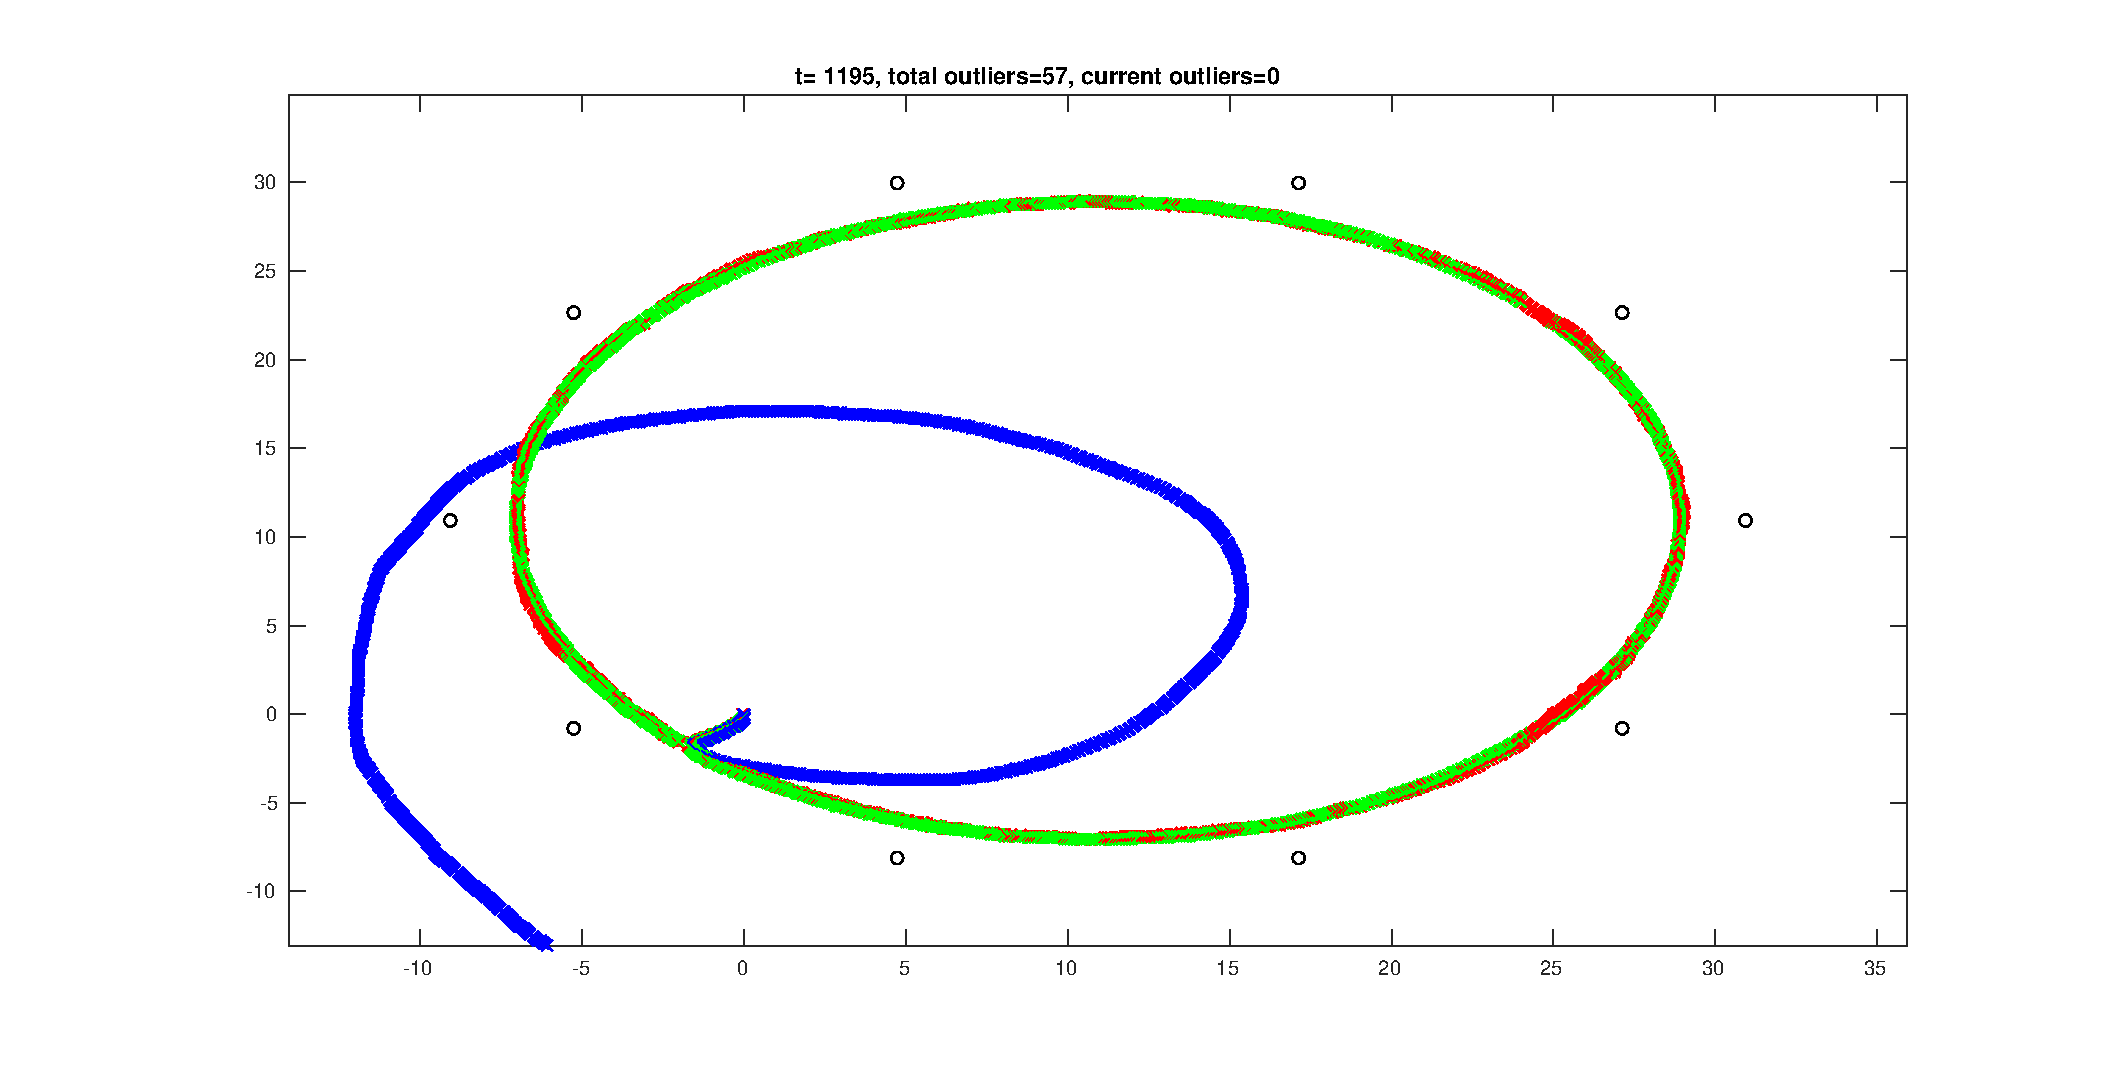
\includegraphics{./figures/part_iii_3/b2.eps}}}
	\caption{Output of the EKF for this experiment.}

	\label{fig:iii3_2}
\end{figure}

Matlab's output for the experiment using batch update was:

\textbf{mean error(x, y, theta)} = (0.007163, 0.004752, -0.012876)

\textbf{mean error(x, y, theta)} = (0.042018, 0.042067, 0.044504)

\textbf{total time} = 94.003578



\subsubsection{map\_pent\_big\_40.txt + so\_pb\_40\_no.txt}

In this experiment the covariance matrices for the process $R$ and measurement noise $Q$ were set to:

\[
R =
\begin{bmatrix}
    1^2  	& 0			& 0 \\
    0       & 1^2 		& 0 \\
    0       & 0 		& 1^2 \\

\end{bmatrix}
\]


\[
Q =
\begin{bmatrix}
    0.1^2  & 0 \\
    0      & 0.1^2 \\

\end{bmatrix}
\]


The vulnerability of the sequential update method to high noise values is clearly illustrated here,
as it is apparent that the EKF cannot track the true state as well as the batch batch update method.
The effect is made more severe, since outliers are not to be rejected.
Notably, the error values in estimation in the sequential update are almost $50$ times larger than
in the batch update.

Figure \ref{fig:iii33_s} shows the output of the EKF for this experiment using sequential update.

\begin{figure}[H]
	\scalebox{0.6}{% This file was created by matlab2tikz.
%
%The latest updates can be retrieved from
%  http://www.mathworks.com/matlabcentral/fileexchange/22022-matlab2tikz-matlab2tikz
%where you can also make suggestions and rate matlab2tikz.
%
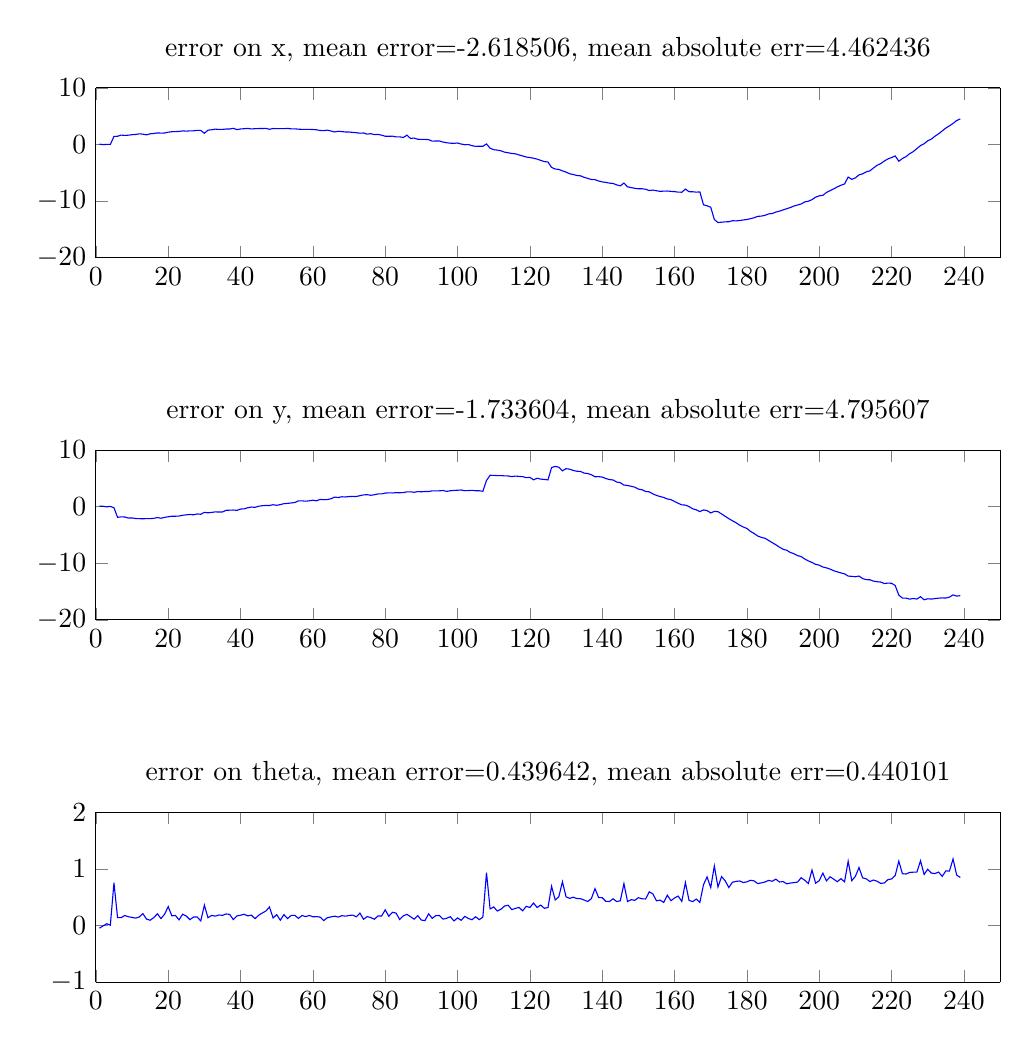
\begin{tikzpicture}

\begin{axis}[%
width=4.521in,
height=0.849in,
at={(0.758in,4.103in)},
scale only axis,
separate axis lines,
every outer x axis line/.append style={black},
every x tick label/.append style={font=\color{black}},
xmin=0,
xmax=250,
every outer y axis line/.append style={black},
every y tick label/.append style={font=\color{black}},
ymin=-20,
ymax=10,
axis background/.style={fill=white},
title={error on x, mean error=-2.618506, mean absolute err=4.462436}
]
\addplot [color=blue,solid,forget plot]
  table[row sep=crcr]{%
1	0.0621834725377347\\
2	-0.0223556805764436\\
3	0.0164279034192492\\
4	0.0099076224068237\\
5	1.42149512676765\\
6	1.45159043571508\\
7	1.65707078480584\\
8	1.59837911414348\\
9	1.64292576978797\\
10	1.72906518284259\\
11	1.77033239072201\\
12	1.8795042779716\\
13	1.82647099265433\\
14	1.70186355288629\\
15	1.88710130066752\\
16	1.94782274986947\\
17	2.03947785046685\\
18	2.00932082994593\\
19	2.02211230498797\\
20	2.17093705452108\\
21	2.25338179170908\\
22	2.28020850815507\\
23	2.30601129196512\\
24	2.40018288464183\\
25	2.35770745549891\\
26	2.40340643229667\\
27	2.41629741354783\\
28	2.50173932314059\\
29	2.49077824994823\\
30	1.98286991356038\\
31	2.53341691649302\\
32	2.5958624828211\\
33	2.71053226725625\\
34	2.65687395334918\\
35	2.6640342054052\\
36	2.72773197672191\\
37	2.73110397428899\\
38	2.85574350227026\\
39	2.62871262376255\\
40	2.73994144979537\\
41	2.78648995575672\\
42	2.83979043929825\\
43	2.7421460804608\\
44	2.78792595659216\\
45	2.81720753705138\\
46	2.82742668160423\\
47	2.83984947278003\\
48	2.68910365495554\\
49	2.81565084840749\\
50	2.8059384186754\\
51	2.79150375317566\\
52	2.78796573805862\\
53	2.84727347633471\\
54	2.75910966907542\\
55	2.7591635939017\\
56	2.70433026165824\\
57	2.66976300855387\\
58	2.65769836829351\\
59	2.66541074567313\\
60	2.64659531654461\\
61	2.59812703098494\\
62	2.47090582581865\\
63	2.44634432971596\\
64	2.53547041435077\\
65	2.37853880886694\\
66	2.20995631509453\\
67	2.32798844678448\\
68	2.28118653478785\\
69	2.20173467851384\\
70	2.19854531626996\\
71	2.13426046724951\\
72	2.07936422012453\\
73	1.99152215216749\\
74	2.02869379712386\\
75	1.82668237786032\\
76	1.90520778401586\\
77	1.74379098598871\\
78	1.78063679025903\\
79	1.64231041740555\\
80	1.45896851248486\\
81	1.44261842253123\\
82	1.46810214799573\\
83	1.33770761202563\\
84	1.35002865413916\\
85	1.22968459342337\\
86	1.64376194032999\\
87	1.06233699311572\\
88	1.13373477104075\\
89	0.917748321888737\\
90	0.90746963613919\\
91	0.899141583852163\\
92	0.851925237756397\\
93	0.586911562004865\\
94	0.61854008338431\\
95	0.615196933606999\\
96	0.42082853702188\\
97	0.303605338468781\\
98	0.227604431962529\\
99	0.20085556857266\\
100	0.263927796834132\\
101	0.0778213112184289\\
102	-0.0428652489686208\\
103	-0.012969477492291\\
104	-0.20985265294501\\
105	-0.331246611239276\\
106	-0.313827778567205\\
107	-0.32207749817476\\
108	0.0961375272506793\\
109	-0.662283849108594\\
110	-0.93024518964976\\
111	-0.99369397712627\\
112	-1.12133305371261\\
113	-1.35397210537731\\
114	-1.46813252555664\\
115	-1.58706091282372\\
116	-1.6546732590118\\
117	-1.84892770047754\\
118	-2.03087863493949\\
119	-2.21797824295775\\
120	-2.31115525863989\\
121	-2.42818197892145\\
122	-2.58691261122321\\
123	-2.8044384131774\\
124	-3.02083991851491\\
125	-3.09480850205931\\
126	-4.05403106206631\\
127	-4.33248227325923\\
128	-4.4115554278718\\
129	-4.65656827828593\\
130	-4.88234527993671\\
131	-5.17719538046637\\
132	-5.30374100921325\\
133	-5.48096730563336\\
134	-5.53657354613714\\
135	-5.81048498454825\\
136	-5.98785929384865\\
137	-6.1888092065187\\
138	-6.21124819575239\\
139	-6.45729208799648\\
140	-6.61079480464166\\
141	-6.69428636534764\\
142	-6.82723540672142\\
143	-6.89139947707947\\
144	-7.13676237952771\\
145	-7.31332607980518\\
146	-6.81293593925997\\
147	-7.48744468863701\\
148	-7.61800169942906\\
149	-7.74235253043218\\
150	-7.82954150066894\\
151	-7.82627667761728\\
152	-7.90728549375755\\
153	-8.14352846030022\\
154	-8.05816260730567\\
155	-8.17607988210391\\
156	-8.27829710627187\\
157	-8.24448664993048\\
158	-8.22276772422696\\
159	-8.28522424372232\\
160	-8.33515457984733\\
161	-8.41594597017599\\
162	-8.43597333208394\\
163	-7.88586881787668\\
164	-8.34156885414245\\
165	-8.35166393345393\\
166	-8.42270744346706\\
167	-8.37958350034122\\
168	-10.6538730629686\\
169	-10.8425542644998\\
170	-11.0802285868382\\
171	-13.2478168170777\\
172	-13.7871305955264\\
173	-13.7324006416414\\
174	-13.6666345336418\\
175	-13.6518181634598\\
176	-13.4708460750911\\
177	-13.5019273064481\\
178	-13.4340308332339\\
179	-13.3372048173037\\
180	-13.2496990210426\\
181	-13.1051526131647\\
182	-12.9418406026521\\
183	-12.6980691325719\\
184	-12.6542803928147\\
185	-12.5184277053139\\
186	-12.2677776389695\\
187	-12.1987766001055\\
188	-11.9448102043153\\
189	-11.7842648262047\\
190	-11.5702999422809\\
191	-11.3571752430805\\
192	-11.1449782017806\\
193	-10.8714370396547\\
194	-10.6968194096061\\
195	-10.5111312268067\\
196	-10.1454982286321\\
197	-10.0218432523204\\
198	-9.74717775849017\\
199	-9.304439219758\\
200	-9.07333583367906\\
201	-8.9830301582251\\
202	-8.48061415090936\\
203	-8.15337020817237\\
204	-7.84610413150489\\
205	-7.4964411300363\\
206	-7.2080137840208\\
207	-6.96784821293401\\
208	-5.75575969609236\\
209	-6.16029258148499\\
210	-5.89859999011342\\
211	-5.36700259570953\\
212	-5.1929493926142\\
213	-4.83325387052142\\
214	-4.66475167877304\\
215	-4.15270057661892\\
216	-3.67868931538975\\
217	-3.38179530313839\\
218	-2.92482150587182\\
219	-2.54715005095094\\
220	-2.31244253193685\\
221	-2.02219019726687\\
222	-2.96562208427472\\
223	-2.48214455084448\\
224	-2.1428730023841\\
225	-1.63248844346639\\
226	-1.25655324117171\\
227	-0.715182330997255\\
228	-0.199584601868185\\
229	0.137118294594437\\
230	0.646147599365122\\
231	0.949278647956192\\
232	1.46069171351979\\
233	1.88412639519719\\
234	2.38508175429796\\
235	2.89617676981368\\
236	3.29671754302406\\
237	3.72583811597939\\
238	4.23268370162753\\
239	4.51900035044352\\
};
\end{axis}

\begin{axis}[%
width=4.521in,
height=0.849in,
at={(0.758in,2.292in)},
scale only axis,
separate axis lines,
every outer x axis line/.append style={black},
every x tick label/.append style={font=\color{black}},
xmin=0,
xmax=250,
every outer y axis line/.append style={black},
every y tick label/.append style={font=\color{black}},
ymin=-20,
ymax=10,
axis background/.style={fill=white},
title={error on y, mean error=-1.733604, mean absolute err=4.795607}
]
\addplot [color=blue,solid,forget plot]
  table[row sep=crcr]{%
1	0.0875983516764358\\
2	0.0736149587663811\\
3	-0.0343121326791419\\
4	0.0525491074246281\\
5	-0.198256270467631\\
6	-1.88186354116234\\
7	-1.79670822218003\\
8	-1.82650531252095\\
9	-2.01310922798141\\
10	-1.99007913667034\\
11	-2.09370264965795\\
12	-2.11840685148699\\
13	-2.13826032457929\\
14	-2.10959463681923\\
15	-2.11871252170461\\
16	-2.06054283183336\\
17	-1.92347969128464\\
18	-2.0456812017893\\
19	-1.89258466536552\\
20	-1.77933624011461\\
21	-1.68658651394521\\
22	-1.68812346382831\\
23	-1.65170060880727\\
24	-1.5226329905205\\
25	-1.44325210068843\\
26	-1.37607325962572\\
27	-1.44094199554325\\
28	-1.28364023203089\\
29	-1.34387772173957\\
30	-1.0004373966712\\
31	-1.08875975502829\\
32	-1.01287583774064\\
33	-0.9247684129425\\
34	-0.94381365601562\\
35	-0.937572393273922\\
36	-0.644797510279075\\
37	-0.61810601194287\\
38	-0.591193848091795\\
39	-0.653553085851687\\
40	-0.423377051679778\\
41	-0.382308623746453\\
42	-0.187736841134043\\
43	-0.0632191454757329\\
44	-0.120737218504369\\
45	0.0773806523331988\\
46	0.16805581959964\\
47	0.218687757504481\\
48	0.209807528661805\\
49	0.345837967342556\\
50	0.236569642777891\\
51	0.369951344169281\\
52	0.535705935116917\\
53	0.581321340148791\\
54	0.654981918528264\\
55	0.731971372113203\\
56	1.01919223168331\\
57	1.02713843396554\\
58	0.967824592473541\\
59	1.03063949629135\\
60	1.13684431585153\\
61	1.03471720386763\\
62	1.28422648342328\\
63	1.2299221314899\\
64	1.25857810102811\\
65	1.39650688438365\\
66	1.68978960922057\\
67	1.61834981212101\\
68	1.75283213601404\\
69	1.71142228125919\\
70	1.7926077833923\\
71	1.81040585890217\\
72	1.79607166715106\\
73	1.94265024069823\\
74	2.07717029337929\\
75	2.12463464816519\\
76	2.01018650579805\\
77	2.10873205558151\\
78	2.24891885697507\\
79	2.25356063539982\\
80	2.40400971748048\\
81	2.44029849938943\\
82	2.42370318321565\\
83	2.47320251801484\\
84	2.4622357835251\\
85	2.48840866620953\\
86	2.61608028928358\\
87	2.62279361622112\\
88	2.54046414049928\\
89	2.66357817463981\\
90	2.62922268248401\\
91	2.68366703189937\\
92	2.67273662573334\\
93	2.80220533039749\\
94	2.80378568878571\\
95	2.80372400996996\\
96	2.85823310489314\\
97	2.69775602811354\\
98	2.81351080255445\\
99	2.87363136275329\\
100	2.90172285873814\\
101	2.94618610785212\\
102	2.82140607629262\\
103	2.84503270913684\\
104	2.88872356173287\\
105	2.81900805108197\\
106	2.81565866100639\\
107	2.71965891640922\\
108	4.6215905524849\\
109	5.5482817190434\\
110	5.52806560891493\\
111	5.49194982880156\\
112	5.49447674813754\\
113	5.44049513119958\\
114	5.42559770528243\\
115	5.31553654946398\\
116	5.40391613286447\\
117	5.34839709017843\\
118	5.30538473183235\\
119	5.12535066369654\\
120	5.17361061501446\\
121	4.74235481912434\\
122	5.01728042259835\\
123	4.87096786727824\\
124	4.81207818086754\\
125	4.72907988266525\\
126	6.91002374924935\\
127	7.10782207657697\\
128	6.97759554513065\\
129	6.3299878941345\\
130	6.71812278921827\\
131	6.62642147178353\\
132	6.3999649935202\\
133	6.25854492029362\\
134	6.22696834026625\\
135	5.92876198697735\\
136	5.86219577453999\\
137	5.64146420610828\\
138	5.28560645487558\\
139	5.30701143824164\\
140	5.23123275379765\\
141	4.9701309092381\\
142	4.79207492249284\\
143	4.71497637050398\\
144	4.3545096509599\\
145	4.24825754863516\\
146	3.81920956757345\\
147	3.74205285682663\\
148	3.60256913784664\\
149	3.45190745768738\\
150	3.10758949257423\\
151	2.99118644721623\\
152	2.68483769138629\\
153	2.61987738482946\\
154	2.26175508627547\\
155	1.98839773786886\\
156	1.79592017921162\\
157	1.62504848519212\\
158	1.35957260064947\\
159	1.25168315043346\\
160	0.907417182816268\\
161	0.598339560110617\\
162	0.316960916098765\\
163	0.282062502741532\\
164	0.0192233872675018\\
165	-0.371198389933731\\
166	-0.555706206919169\\
167	-0.866346126307228\\
168	-0.572910885534061\\
169	-0.693117303452354\\
170	-1.10596090315261\\
171	-0.834192522442248\\
172	-0.879530264645002\\
173	-1.28203828640813\\
174	-1.69986443519439\\
175	-2.11570317060924\\
176	-2.48162099808669\\
177	-2.83594466711023\\
178	-3.26450095701029\\
179	-3.59431416363201\\
180	-3.84550524650538\\
181	-4.36929303223297\\
182	-4.73553806879277\\
183	-5.18487792523316\\
184	-5.42209894278364\\
185	-5.57809326909093\\
186	-5.96514889374601\\
187	-6.34960260770469\\
188	-6.73074391473246\\
189	-7.14740743870808\\
190	-7.52629579010287\\
191	-7.69582779062375\\
192	-8.08613293562526\\
193	-8.31414898835968\\
194	-8.64643941306356\\
195	-8.81612606497663\\
196	-9.24537942134674\\
197	-9.58835963295802\\
198	-9.85799602860015\\
199	-10.1901817795095\\
200	-10.3275223481715\\
201	-10.6564581974257\\
202	-10.8158287996658\\
203	-11.0268974307398\\
204	-11.3188980777758\\
205	-11.5141868754304\\
206	-11.7084067979263\\
207	-11.862151439998\\
208	-12.2620846189803\\
209	-12.3127063563198\\
210	-12.3799316388339\\
211	-12.2555164069706\\
212	-12.7029843374932\\
213	-12.894264867904\\
214	-12.9168218733374\\
215	-13.1544371163675\\
216	-13.2589871821801\\
217	-13.3170820607526\\
218	-13.5807428702692\\
219	-13.4999026072965\\
220	-13.5330433876187\\
221	-13.9251623659277\\
222	-15.6259099397367\\
223	-16.1575131985097\\
224	-16.1554549906647\\
225	-16.3362814224302\\
226	-16.2205484545681\\
227	-16.3243650972546\\
228	-15.9042099618892\\
229	-16.4527523554862\\
230	-16.2722609049353\\
231	-16.3251758131957\\
232	-16.2348563111483\\
233	-16.1660153412798\\
234	-16.1186921733981\\
235	-16.1376984028666\\
236	-15.976138868622\\
237	-15.5864798235943\\
238	-15.7970635258678\\
239	-15.7258931952391\\
};
\end{axis}

\begin{axis}[%
width=4.521in,
height=0.849in,
at={(0.758in,0.481in)},
scale only axis,
separate axis lines,
every outer x axis line/.append style={black},
every x tick label/.append style={font=\color{black}},
xmin=0,
xmax=250,
every outer y axis line/.append style={black},
every y tick label/.append style={font=\color{black}},
ymin=-1,
ymax=2,
axis background/.style={fill=white},
title={error on theta, mean error=0.439642, mean absolute err=0.440101}
]
\addplot [color=blue,solid,forget plot]
  table[row sep=crcr]{%
1	-0.0471806770241319\\
2	-0.00767769315902056\\
3	0.0308136785404201\\
4	0.00466820535103452\\
5	0.75451926494088\\
6	0.137742298494452\\
7	0.138715885280931\\
8	0.175983334535808\\
9	0.154475750628985\\
10	0.1424557822182\\
11	0.129695172974606\\
12	0.150729180227375\\
13	0.209573661754427\\
14	0.112408868939817\\
15	0.0929297290363698\\
16	0.13833265969901\\
17	0.206790716885544\\
18	0.121665864088217\\
19	0.197845895518539\\
20	0.332979376920756\\
21	0.170495297710591\\
22	0.17720109449366\\
23	0.0993648634891642\\
24	0.199215703294981\\
25	0.16646816368432\\
26	0.103155493050874\\
27	0.149261132198032\\
28	0.151109100206416\\
29	0.0805072560414968\\
30	0.358789251792441\\
31	0.13655682102502\\
32	0.178293846804928\\
33	0.164442862194428\\
34	0.185177023805431\\
35	0.178587868559199\\
36	0.202994082473049\\
37	0.196400107453281\\
38	0.103190836392264\\
39	0.167601234928732\\
40	0.181532550687471\\
41	0.197732563505583\\
42	0.169955713055443\\
43	0.182216961279899\\
44	0.119881681360448\\
45	0.179894001536672\\
46	0.219877829511097\\
47	0.254881217558027\\
48	0.326440152902139\\
49	0.132461973344713\\
50	0.191154481603836\\
51	0.0937916670967791\\
52	0.191283676862157\\
53	0.12164023698143\\
54	0.177237314238325\\
55	0.179531886429328\\
56	0.12549639634248\\
57	0.176431403765358\\
58	0.156232069989238\\
59	0.17785045526246\\
60	0.153793262997071\\
61	0.156327038433344\\
62	0.148099979072478\\
63	0.0859371671927294\\
64	0.136961923698807\\
65	0.151006127926313\\
66	0.164941967854841\\
67	0.148072081019206\\
68	0.173431074606861\\
69	0.164153402976149\\
70	0.176957711554526\\
71	0.183396059670051\\
72	0.15247213619272\\
73	0.218084486781482\\
74	0.110153409821172\\
75	0.15761190254954\\
76	0.139711447769449\\
77	0.109665792621533\\
78	0.168177423291838\\
79	0.166604785348241\\
80	0.275794271085213\\
81	0.162825872282088\\
82	0.233181152290688\\
83	0.218643799494685\\
84	0.106183034068767\\
85	0.169014834429121\\
86	0.196407200112052\\
87	0.154127138601575\\
88	0.112110207491132\\
89	0.175283990159584\\
90	0.0948321709853834\\
91	0.0873539745308474\\
92	0.205925830814267\\
93	0.125718523269379\\
94	0.174662332575366\\
95	0.175798850054078\\
96	0.112269605452226\\
97	0.12764242485498\\
98	0.154926563757641\\
99	0.0800014602016992\\
100	0.133838135532775\\
101	0.0914241553389106\\
102	0.160819030210495\\
103	0.123401744049391\\
104	0.102354209117976\\
105	0.153551350816727\\
106	0.103027509284984\\
107	0.146990038241868\\
108	0.933908402107355\\
109	0.292585187899936\\
110	0.327424603146038\\
111	0.254798191427149\\
112	0.286809597232548\\
113	0.343697341705293\\
114	0.357662499336121\\
115	0.280241638237865\\
116	0.301716684870388\\
117	0.319564628275021\\
118	0.25851691943129\\
119	0.338749800393467\\
120	0.318418324460884\\
121	0.395413780224879\\
122	0.318238727233798\\
123	0.360043281993118\\
124	0.303909463259952\\
125	0.31641370929287\\
126	0.692188710158256\\
127	0.451130996261463\\
128	0.507625074592812\\
129	0.771840256890688\\
130	0.506068880025334\\
131	0.478724636295912\\
132	0.498821343457552\\
133	0.4763772717654\\
134	0.472718309269279\\
135	0.450239392180193\\
136	0.422822691281598\\
137	0.474696203058423\\
138	0.649711788911781\\
139	0.494236377087294\\
140	0.490780687674209\\
141	0.426099668892446\\
142	0.424072683453575\\
143	0.471217301233548\\
144	0.422726724645906\\
145	0.436197951831495\\
146	0.739098865593431\\
147	0.422116557687104\\
148	0.456274391946398\\
149	0.444146847007871\\
150	0.490959034736666\\
151	0.471920179066796\\
152	0.468047967514716\\
153	0.59407985672257\\
154	0.558782970606405\\
155	0.435723995459428\\
156	0.448325502872123\\
157	0.406869336686993\\
158	0.535055787759912\\
159	0.437995728457608\\
160	0.485522724493281\\
161	0.519537693847146\\
162	0.425223996875241\\
163	0.759466376556247\\
164	0.443301253629254\\
165	0.42148463539238\\
166	0.466577410709071\\
167	0.408038474518921\\
168	0.720658039787265\\
169	0.858074406682016\\
170	0.667997077242084\\
171	1.05091168478241\\
172	0.679481609209436\\
173	0.863931048115484\\
174	0.78821453196244\\
175	0.671572058240899\\
176	0.763326570793015\\
177	0.779078357766481\\
178	0.786002772132811\\
179	0.758523601784889\\
180	0.771271869428763\\
181	0.798167212755698\\
182	0.787938347117684\\
183	0.739777689483789\\
184	0.752622056396664\\
185	0.76798645273091\\
186	0.79673120503223\\
187	0.78147385224884\\
188	0.818894842767089\\
189	0.768211212534601\\
190	0.775792411842195\\
191	0.736030866942809\\
192	0.749233079738504\\
193	0.757312737797037\\
194	0.766630966594684\\
195	0.843972865854623\\
196	0.799021434545637\\
197	0.741218917796991\\
198	0.979354397357998\\
199	0.747268413375227\\
200	0.791001849732652\\
201	0.924881277659675\\
202	0.788620141199755\\
203	0.860452299848594\\
204	0.817738417213352\\
205	0.773476956457656\\
206	0.827025823440829\\
207	0.771089264137724\\
208	1.1352080753475\\
209	0.791223437228967\\
210	0.868964194103504\\
211	1.02387700427776\\
212	0.840905787854715\\
213	0.823831522355345\\
214	0.775392204290963\\
215	0.803053797653155\\
216	0.781809346947112\\
217	0.74353323383184\\
218	0.751327177164284\\
219	0.810483861845513\\
220	0.821798004865502\\
221	0.882048889791345\\
222	1.13663862490689\\
223	0.914631299116832\\
224	0.909165804731127\\
225	0.937381245348913\\
226	0.941355694304329\\
227	0.941814992114729\\
228	1.14306704812874\\
229	0.90163290969865\\
230	0.993290115128157\\
231	0.924443395676921\\
232	0.91753067395187\\
233	0.942797662842767\\
234	0.867800501864164\\
235	0.964457474700162\\
236	0.96040529672616\\
237	1.17488808115201\\
238	0.890468115672458\\
239	0.847742190466197\\
};
\end{axis}
\end{tikzpicture}%}
	\scalebox{0.6}{\input{./figures/part_iii_3/so_pb_40_no_map_pent_big_40_sequential_3}}

	\centering
	\centerline{\scalebox{0.5}{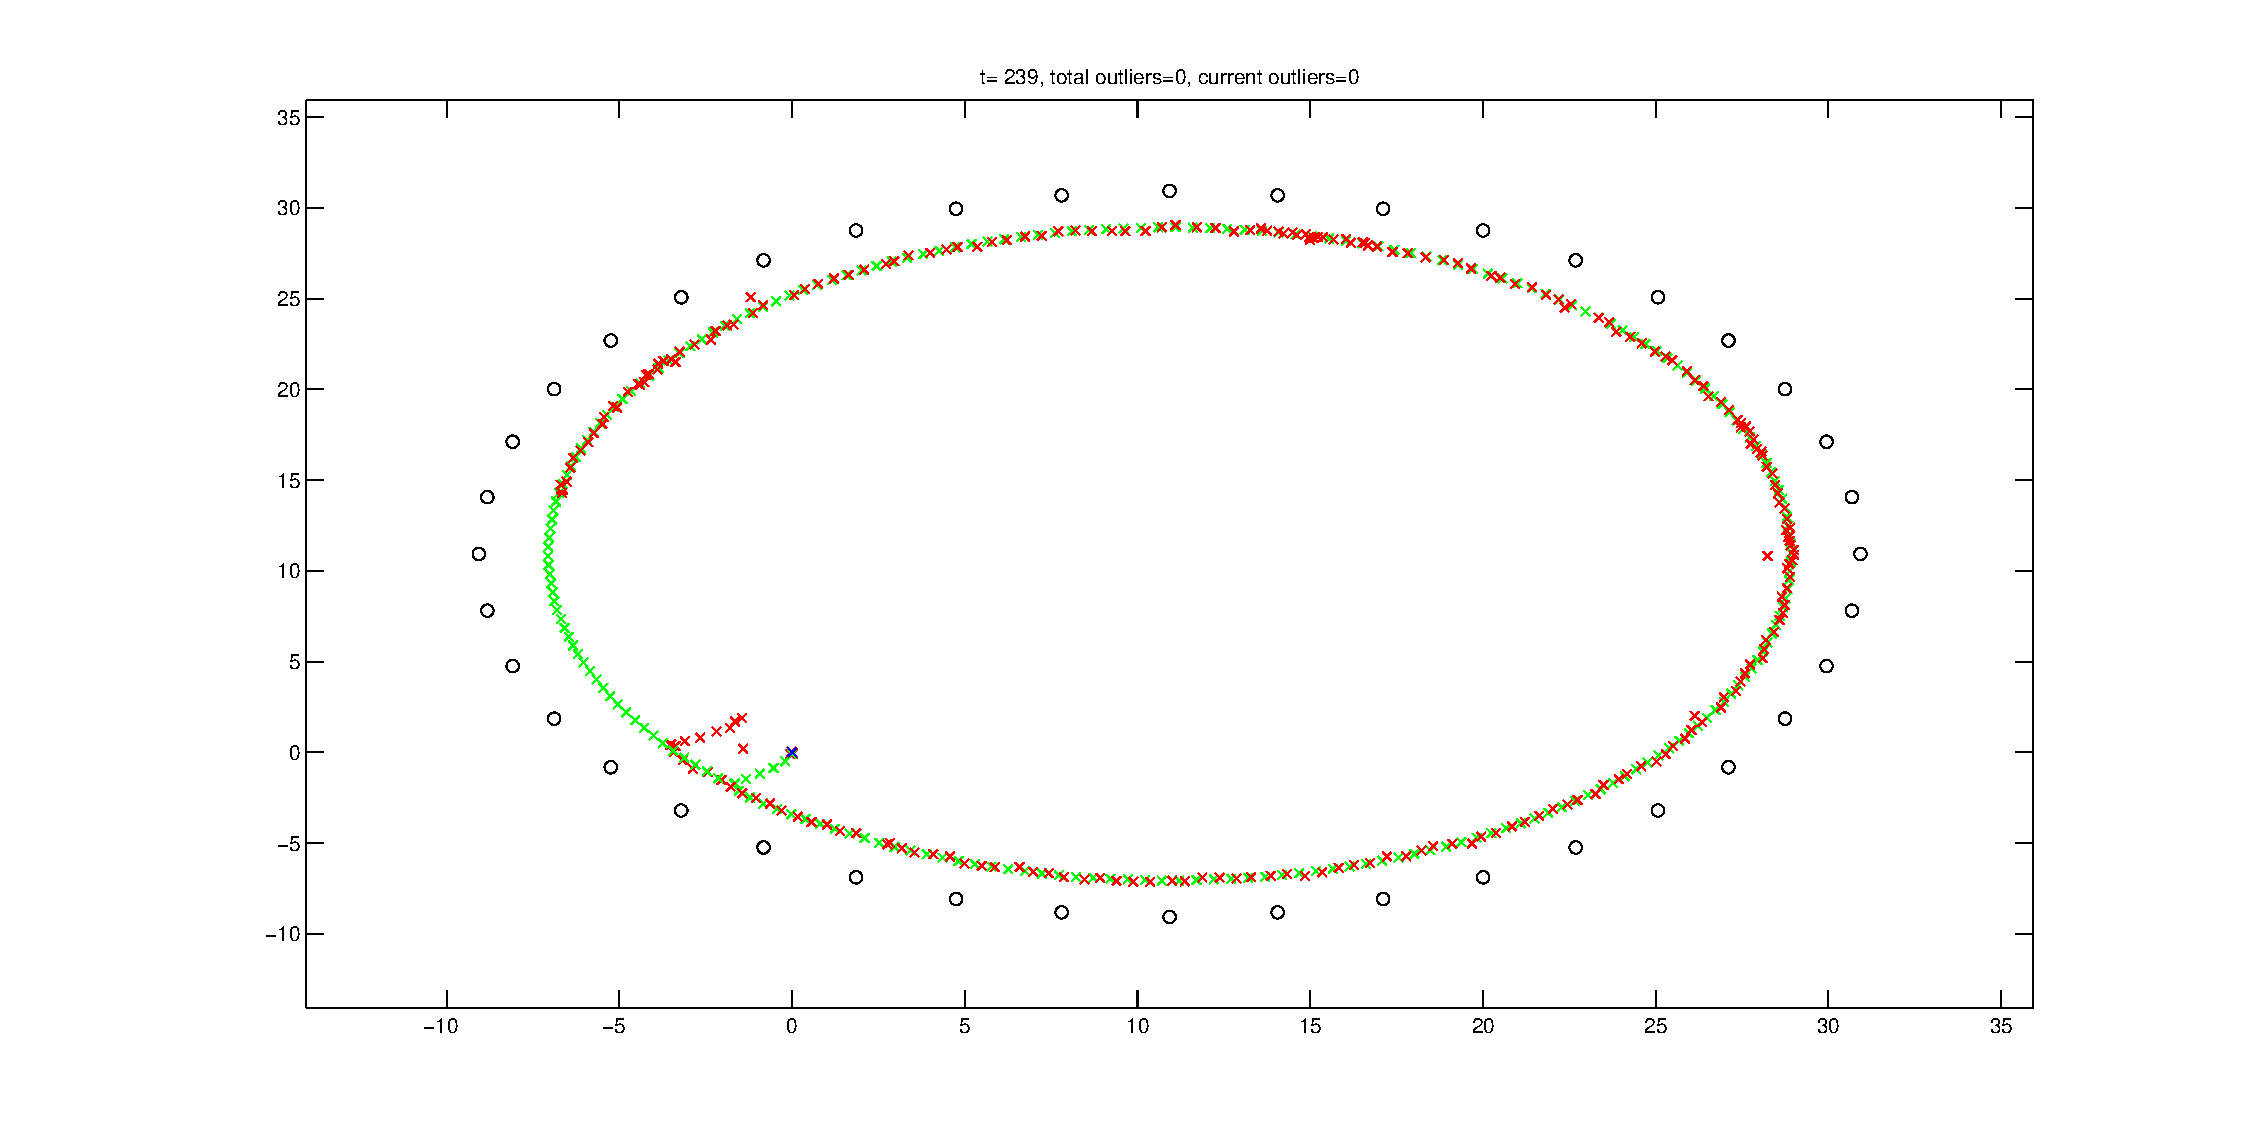
\includegraphics{./figures/part_iii_3/s3.eps}}}

	\caption{Output of the EKF for this experiment using sequential update.}
	\label{fig:iii33_s}
\end{figure}

Matlab's output for the experiment was:

\textbf{mean error(x, y, theta)} = (-2.618506, -1.733604, 0.439642)

\textbf{mean absolute error} = (4.462436, 4.795607, 0.440101)

\textbf{total time} = 18.211545


Conversely, the batch update method's nature of associating all measurements with the landmarks simultaneously
proves to be impervious to high noise. Furthermore, the fact that outliers are not rejected furthers the claim of robustness of the method.
Notably, the computational cost is not only comparable but even less than that of the sequential method in terms of execution time.

Figure \ref{fig:iii33_b} shows the output of the EKF for this experiment using batch update.

\begin{figure}[H]
	\scalebox{0.6}{% This file was created by matlab2tikz.
%
%The latest updates can be retrieved from
%  http://www.mathworks.com/matlabcentral/fileexchange/22022-matlab2tikz-matlab2tikz
%where you can also make suggestions and rate matlab2tikz.
%
\definecolor{mycolor1}{rgb}{0.00000,0.44700,0.74100}%
%
\begin{tikzpicture}

\begin{axis}[%
width=4.521in,
height=0.849in,
at={(0.758in,4.103in)},
scale only axis,
xmin=0,
xmax=250,
ymin=-1,
ymax=1,
axis background/.style={fill=white},
title style={font=\bfseries},
title={error on x, mean error=-0.026019, mean absolute err=0.080351}
]
\addplot [color=mycolor1,solid,forget plot]
  table[row sep=crcr]{%
1	0.0657935555963038\\
2	-0.0205706856231176\\
3	0.0247233608234243\\
4	0.0187360972494681\\
5	-0.105318371645915\\
6	-0.280438487652861\\
7	0.0609349004411845\\
8	-0.0492041297555194\\
9	-0.0497838656099918\\
10	0.00976508676797039\\
11	-0.0181119173841533\\
12	0.0538548630157942\\
13	0.00964004582772549\\
14	-0.104066207894845\\
15	0.00439169012821039\\
16	-0.0428654958973755\\
17	-0.00386155426293278\\
18	-0.0466369907122963\\
19	-0.107209811522172\\
20	0.00483559398514166\\
21	0.00432558444322195\\
22	0.00747422882324278\\
23	-0.00620154630880143\\
24	0.0368775890141086\\
25	-0.0588443942076249\\
26	-0.0547458773235419\\
27	-0.0466325987300729\\
28	-0.0124271008966321\\
29	-0.0303684665196462\\
30	-0.0536609845692366\\
31	-0.0953423152556594\\
32	-0.0405717048821845\\
33	0.0421723375241099\\
34	-0.00847898333457398\\
35	-0.0262544485411356\\
36	-0.0278208070234909\\
37	-0.0286805744437615\\
38	0.0932539508476502\\
39	-0.117737045823658\\
40	-0.0547967476924018\\
41	-0.00641586398381122\\
42	0.0447961640035661\\
43	-0.0816516420337354\\
44	-0.0249765545409151\\
45	-0.0224883057746972\\
46	-0.0085024837146932\\
47	0.0185204641799235\\
48	-0.0908911956304124\\
49	0.000192241113900593\\
50	0.0503612873730699\\
51	0.0247018169292019\\
52	0.0259605214953051\\
53	0.101277686667437\\
54	0.0343516289994916\\
55	0.0574447672161256\\
56	-0.0131390724954805\\
57	-0.00531888132663028\\
58	0.0448268137316354\\
59	0.060153850462175\\
60	0.0702071706740526\\
61	0.0875356573088482\\
62	-0.0294996582242746\\
63	0.00527392714116459\\
64	0.105083568836768\\
65	0.00630698882276093\\
66	-0.151863383519466\\
67	0.0253917463223381\\
68	0.00628619295374122\\
69	0.016985359234738\\
70	0.0330331515759958\\
71	0.0357271329752429\\
72	0.0442775139891829\\
73	-0.00973851036169648\\
74	0.0606714441533569\\
75	-0.0548655207348965\\
76	0.113977142191004\\
77	0.00510859436339572\\
78	0.0666116437596536\\
79	0.0156930522250178\\
80	-0.131329308628665\\
81	-0.0691842592351932\\
82	0.0384331957533632\\
83	-0.00904456724801506\\
84	0.044941201421711\\
85	0.000141433692636639\\
86	0.230889564108754\\
87	0.0112955120452476\\
88	0.135400614872463\\
89	-0.0230721306708261\\
90	0.0461342114498642\\
91	0.0928977859475673\\
92	0.140982348154381\\
93	-0.0623107667345622\\
94	0.0349279609078721\\
95	0.12096740686092\\
96	-0.00139224420498607\\
97	-0.0248786309336531\\
98	-0.0576299376872562\\
99	-0.00833006538206149\\
100	0.112070598875906\\
101	0.0118285429648814\\
102	0.00299326244990539\\
103	0.112222372197312\\
104	-0.0249857654151207\\
105	-0.0342585888315945\\
106	0.0639672535865756\\
107	0.146111363874869\\
108	-0.313523554345387\\
109	0.12811710766745\\
110	-0.0191908558258405\\
111	0.0151582519635447\\
112	0.066091082120213\\
113	0.00898288214057175\\
114	0.018913527747948\\
115	0.0778599153084549\\
116	0.0914417224529878\\
117	0.0784299064752112\\
118	0.0457428818997343\\
119	0.0490488669442719\\
120	0.0282857059127579\\
121	0.165700110355584\\
122	0.0236664833707252\\
123	0.00506677168357328\\
124	-0.0880117276231474\\
125	-0.0580169008838922\\
126	-0.307959735620663\\
127	0.193584681592935\\
128	0.14244410310852\\
129	0.124426155948509\\
130	0.138445479251597\\
131	-0.00768571692942643\\
132	0.081544859050652\\
133	0.0866216234064652\\
134	0.115239821682415\\
135	0.0663138974218747\\
136	0.0312993837223061\\
137	0.035189292144544\\
138	0.110593945993884\\
139	0.0257227340545505\\
140	-0.0161359269010859\\
141	0.0818544849211236\\
142	0.0612078660690152\\
143	0.0817431665592459\\
144	0.0601547094589279\\
145	-0.0470097617881144\\
146	0.396822605780812\\
147	0.0283838166682315\\
148	-0.0389201882606329\\
149	-0.0739220025264071\\
150	-0.00678588021932214\\
151	0.0168484168971688\\
152	0.0368300408257305\\
153	-0.172366071884527\\
154	0.0304571267425828\\
155	0.0055189062792298\\
156	-0.0585038046100212\\
157	-0.0262959585705822\\
158	0.0494976319250089\\
159	-0.0338808002552042\\
160	0.00541229765260809\\
161	-0.0152913274223003\\
162	0.000431383861787538\\
163	-0.251799171471562\\
164	0.00911521543506488\\
165	0.0628644223344077\\
166	-0.0163235961891663\\
167	0.0346942515335504\\
168	-0.450932984352466\\
169	-0.460336625368911\\
170	-0.0486503425281808\\
171	-0.376079074836464\\
172	-0.0440453302471262\\
173	-0.104438711167285\\
174	-0.0453217367878018\\
175	-0.0330537963721993\\
176	0.0119638099080139\\
177	-0.0562299464738985\\
178	-0.0257995848796018\\
179	-0.0798039969923967\\
180	-0.174569604426835\\
181	-0.0387321713891076\\
182	-0.00506500135680388\\
183	0.123572663887564\\
184	-0.0275264127750685\\
185	-0.174874286701116\\
186	-0.0974809501311693\\
187	-0.122111365801391\\
188	-0.0581634073327804\\
189	-0.0087727608752175\\
190	0.0086468597693754\\
191	-0.0822967193338426\\
192	-0.0283228987025419\\
193	-0.066946467548699\\
194	-0.0591809258842133\\
195	-0.205341190927906\\
196	-0.0417807668653118\\
197	-0.0614005891678095\\
198	-0.0945490328354017\\
199	0.0479770327576068\\
200	-0.0339055055622373\\
201	-0.123727415477657\\
202	-0.0815710119555817\\
203	-0.0339495063826982\\
204	0.0246397988391802\\
205	0.0177191527871026\\
206	-0.0349335136463145\\
207	-0.0975845957190762\\
208	-0.267326158438475\\
209	0.0196642193002878\\
210	-0.0925703888785927\\
211	-0.380269957957326\\
212	-0.0982465977529507\\
213	-0.0519788799235146\\
214	-0.245579036798995\\
215	-0.0648933559330649\\
216	0.0133703370962159\\
217	-0.0639817168833261\\
218	0.111037040045133\\
219	-0.00170635202533909\\
220	-0.0991092505319298\\
221	0.123066127593121\\
222	-0.0308473402301868\\
223	-0.67512971660284\\
224	-0.80206826984492\\
225	-0.590085577549536\\
226	-0.639148283310957\\
227	-0.470279739592209\\
228	0.051073247969958\\
229	-0.0571638936236214\\
230	-0.0691702599171844\\
231	-0.0384170285039147\\
232	-0.0681602847406859\\
233	-0.0952529158895388\\
234	-0.0755791988249834\\
235	0.0478388435469403\\
236	-0.0391249904978732\\
237	-0.197351999901184\\
238	0.0326774649971866\\
239	-0.03231048662097\\
};
\end{axis}

\begin{axis}[%
width=4.521in,
height=0.849in,
at={(0.758in,2.292in)},
scale only axis,
xmin=0,
xmax=250,
ymin=-1,
ymax=1,
axis background/.style={fill=white},
title style={font=\bfseries},
title={error on y, mean error=-0.022660, mean absolute err=0.088318}
]
\addplot [color=mycolor1,solid,forget plot]
  table[row sep=crcr]{%
1	0.0885654064114234\\
2	0.0738512091638033\\
3	-0.028742665049404\\
4	0.0520585969774265\\
5	0.0258681078253862\\
6	-0.165582378742704\\
7	0.0545966268344957\\
8	0.0495472581454766\\
9	-0.0911642109552097\\
10	0.0100641906394219\\
11	-0.0378880850265755\\
12	-0.00411731265287374\\
13	-0.0109942678887691\\
14	-0.0036218282048901\\
15	-0.00929385980437791\\
16	-0.0269941611411015\\
17	0.0673474951145696\\
18	-0.134003018014671\\
19	-0.0487312802790836\\
20	0.0104607823970282\\
21	0.0411618654537844\\
22	-0.0140692379344705\\
23	-0.0369405876570337\\
24	0.039259473884333\\
25	0.017194828735053\\
26	0.0233313548396534\\
27	-0.106549683207869\\
28	-1.05383331368003e-05\\
29	-0.13785716465669\\
30	-0.318029443940322\\
31	-0.0592416487495138\\
32	-0.0131732838368004\\
33	-0.0155862703416076\\
34	-0.116262205276211\\
35	-0.186166160382617\\
36	0.0350464256180221\\
37	-0.0240065441760695\\
38	-0.0268238017746301\\
39	-0.259930000907497\\
40	-0.0407817740125838\\
41	-0.0863066326915458\\
42	0.0347496613672655\\
43	0.0445606168888295\\
44	-0.0662725843512222\\
45	0.0699938149841124\\
46	0.0879378960337638\\
47	0.0682286591140704\\
48	-0.0726136942477114\\
49	0.0263362119609614\\
50	-0.167021616813583\\
51	-0.110204066274684\\
52	-0.0148743960993949\\
53	-0.0399808613017285\\
54	-0.0700162221321099\\
55	-0.0447125569230282\\
56	0.142087257392463\\
57	0.0874385914425861\\
58	-0.0583995865693421\\
59	-0.0420102682622776\\
60	-0.0141954112270248\\
61	-0.188685151893364\\
62	-0.0404317581305786\\
63	-0.145781213503255\\
64	-0.109303071313076\\
65	-0.120187763853999\\
66	0.0736530456444644\\
67	-0.000804939827398599\\
68	0.0606941443181976\\
69	-0.0611823196931573\\
70	-0.0116937416165315\\
71	-0.0677757747032151\\
72	-0.120039478973238\\
73	-0.0512648789729231\\
74	0.0538280516922747\\
75	0.0123146026816992\\
76	-0.13541863576044\\
77	-0.116292440820853\\
78	0.0150579001317699\\
79	-0.0506424584635068\\
80	0.0397348740270529\\
81	0.0393085750887674\\
82	-0.0105001036020624\\
83	-0.00546284342107661\\
84	-0.0253227191539502\\
85	-0.04666489399201\\
86	0.279749258688652\\
87	-0.00589765005254339\\
88	-0.0775637132021938\\
89	-0.00506788008866099\\
90	-0.0465736127614358\\
91	-0.00297810114012798\\
92	-0.0398174177488846\\
93	0.030948926859903\\
94	0.0387710790093099\\
95	0.0381983171586242\\
96	0.0556821500331299\\
97	-0.1235299453521\\
98	-0.00883475670623568\\
99	0.0512522949488847\\
100	0.102085054003618\\
101	0.125628365154418\\
102	0.000415578164673747\\
103	0.046369746178069\\
104	0.0665626786342894\\
105	0.00156530040048075\\
106	0.0274650338462674\\
107	-0.0468684904948251\\
108	0.212474021769586\\
109	0.0229435475715469\\
110	-0.0517799007283131\\
111	-0.0309570155379859\\
112	0.0162506406116449\\
113	-0.0147566107807791\\
114	0.00761816380117253\\
115	-0.0436563196354385\\
116	0.0916302431584448\\
117	0.0890119199240722\\
118	0.0970379178215417\\
119	-0.0313644244050764\\
120	0.0786366212064316\\
121	-0.152422028788962\\
122	0.0510285570728826\\
123	-0.013216801326795\\
124	-0.0279308931138402\\
125	0.0149453302038403\\
126	0.485962647521983\\
127	0.0727688188567122\\
128	0.00409065799559372\\
129	0.309409508634676\\
130	0.0126995342539686\\
131	-0.0172278972283273\\
132	-0.0516018347312794\\
133	-0.0386469658328608\\
134	0.113371443261599\\
135	-0.0490491936473241\\
136	0.0262258889322844\\
137	-0.0197504352042728\\
138	-0.128303849286812\\
139	-0.000297541846112637\\
140	0.0892836516794659\\
141	0.0741231158909592\\
142	0.0511631407539639\\
143	0.209606897929429\\
144	0.00983189462262501\\
145	0.0504498737302548\\
146	-0.0364239345040822\\
147	-0.0294626397771687\\
148	0.0157006404460631\\
149	0.0839595519749317\\
150	-0.018755680244368\\
151	0.130507395421915\\
152	-0.0481134881677505\\
153	0.0933384941157058\\
154	0.0904171208336031\\
155	-0.0281723739032884\\
156	-0.00302534332476156\\
157	0.0823604596141294\\
158	0.0808520732694689\\
159	0.134909053507251\\
160	0.0604843391261873\\
161	-0.0334744317415989\\
162	-0.0743163026340383\\
163	0.328003402337679\\
164	0.153623801199732\\
165	-0.0324593781719464\\
166	-0.0372789929678525\\
167	-0.0794512449211098\\
168	-0.213822699116438\\
169	0.24621082843624\\
170	-0.0201206947983152\\
171	-0.218753004706347\\
172	-0.415745989079561\\
173	0.0764083126724806\\
174	0.0403120219741417\\
175	-0.0509902765618548\\
176	0.076151190947833\\
177	0.0167264077702391\\
178	-0.0256909554364029\\
179	0.0161756620746694\\
180	0.0649479325989724\\
181	-0.0168897022270436\\
182	0.00187357017276923\\
183	0.0395304481608605\\
184	0.0352698041422848\\
185	0.126631419650789\\
186	0.183464939038121\\
187	0.0577374005380342\\
188	0.0832894332170859\\
189	0.0117812811086715\\
190	-0.0224763401116341\\
191	0.0647704750147788\\
192	0.00825435477886316\\
193	0.0956659179362198\\
194	0.0250408527299122\\
195	0.0828451806564807\\
196	0.0697212898263757\\
197	-0.0910528148844811\\
198	-0.0818255682338531\\
199	0.00171763838535099\\
200	0.0377785019165771\\
201	-0.188442031167583\\
202	0.0454578023053109\\
203	0.058837320431353\\
204	0.00452712350192108\\
205	0.0484764888197073\\
206	0.0448039178746598\\
207	-0.00716133752433379\\
208	-0.0707291570047772\\
209	0.029361650401146\\
210	0.0341757588894467\\
211	-0.127242663658663\\
212	0.0484145275644572\\
213	-0.0106730803233894\\
214	-0.0756746809394642\\
215	-0.0459433125577888\\
216	0.0385157652584081\\
217	0.0196810999600689\\
218	-0.0413003661666611\\
219	0.0495885050578027\\
220	-0.02788140669601\\
221	-0.305602453299621\\
222	-0.662465670730433\\
223	-0.825405709988131\\
224	-0.795610631249653\\
225	-0.924806962090092\\
226	-0.81720646506409\\
227	-0.611521312645181\\
228	-0.700982735932281\\
229	-0.112906868870918\\
230	0.0539392930756799\\
231	-0.0914118665133956\\
232	-0.0298323820574977\\
233	-0.0308719499256941\\
234	0.00806501889366784\\
235	0.000241972778825927\\
236	-0.010747181554256\\
237	0.112007419153794\\
238	0.0340801738856928\\
239	-0.130437181754833\\
};
\end{axis}

\begin{axis}[%
width=4.521in,
height=0.849in,
at={(0.758in,0.481in)},
scale only axis,
xmin=0,
xmax=250,
ymin=-0.5,
ymax=0.5,
axis background/.style={fill=white},
title style={font=\bfseries},
title={error on theta, mean error=0.018390, mean absolute err=0.047883}
]
\addplot [color=mycolor1,solid,forget plot]
  table[row sep=crcr]{%
1	-0.0468230702972661\\
2	-0.00760000870506383\\
3	0.0317247141638726\\
4	0.00515653487846857\\
5	0.0859708217276096\\
6	-0.100325099453571\\
7	-0.0184345276761837\\
8	0.0199512624302658\\
9	-0.0028281600573008\\
10	-0.0129463538243235\\
11	-0.0277125027534488\\
12	-0.00674983336091994\\
13	0.0532815806642377\\
14	-0.0439670602547961\\
15	-0.0632289432162318\\
16	-0.017514395657575\\
17	0.0548220437646885\\
18	-0.0366960848585238\\
19	0.0402238775610524\\
20	0.178424518125776\\
21	0.0142869128209897\\
22	0.0215906040484519\\
23	-0.0568720010136268\\
24	0.0419924633925932\\
25	0.0080522804490708\\
26	-0.0542529877589257\\
27	-0.00694068530082381\\
28	-0.00195931557745554\\
29	-0.0767080729268788\\
30	0.20967613218871\\
31	-0.0215100972969258\\
32	0.0231742757645561\\
33	0.010205360681216\\
34	0.0336568304372142\\
35	0.0215173039867067\\
36	0.0461188466047919\\
37	0.0392281837104811\\
38	-0.0524792514641534\\
39	0.0137536257752537\\
40	0.0280683624403526\\
41	0.042363961158284\\
42	0.0135423255519322\\
43	0.0257177177861094\\
44	-0.0365033986241392\\
45	0.0267370475780315\\
46	0.0636796280930341\\
47	0.0981472456225827\\
48	0.169269479339882\\
49	-0.023848647174959\\
50	0.0387795580778958\\
51	-0.0625318752898001\\
52	0.0366673487435927\\
53	-0.0348903498746762\\
54	0.0200495406733525\\
55	0.0276951622832513\\
56	-0.0283018361912668\\
57	0.0199586041966251\\
58	-0.000304197630494052\\
59	0.0212521354414466\\
60	-0.00263606442008557\\
61	0.00127407741090302\\
62	-0.00688918096590463\\
63	-0.0704941370862922\\
64	-0.0173122423059398\\
65	-0.00652837770144554\\
66	0.0081629821929976\\
67	-0.00821691994447082\\
68	0.018393712345953\\
69	0.00644558503998383\\
70	0.0193282660407315\\
71	0.0268558493579381\\
72	-0.0020806329299794\\
73	0.0624520790295882\\
74	-0.0455197945864123\\
75	0.000387313387516297\\
76	-0.0178900055936397\\
77	-0.0475985753726897\\
78	0.0125304421200614\\
79	0.0131458425968645\\
80	0.120051195894506\\
81	0.0049969858430452\\
82	0.0762743899889768\\
83	0.0615642003594985\\
84	-0.0497256187223654\\
85	0.0137754488809367\\
86	0.0644044436848241\\
87	-0.0040191479247067\\
88	-0.0432585115703237\\
89	0.0183010458147863\\
90	-0.0603828637644108\\
91	-0.0692617524018759\\
92	0.0493922028797646\\
93	-0.0311840187737955\\
94	0.0202699666552535\\
95	0.0218026741043191\\
96	-0.0403150789054392\\
97	-0.0209277960018843\\
98	-0.000233025521518826\\
99	-0.0760881766725401\\
100	-0.0244951441937284\\
101	-0.0649308864267022\\
102	0.00162804803926075\\
103	-0.0360622653326432\\
104	-0.0556414265252956\\
105	-0.004772611816795\\
106	-0.0539241939876938\\
107	-0.00891634585882173\\
108	0.231340308889186\\
109	-0.0255054978054758\\
110	0.0141491849540838\\
111	-0.046197406237769\\
112	-0.0250423434571245\\
113	0.0336642498251103\\
114	0.0441095024290705\\
115	-0.0349192795908686\\
116	-0.0125686983596913\\
117	0.0055362175093836\\
118	-0.0548659319654212\\
119	0.0257990163162192\\
120	0.00447170957656251\\
121	0.0977241277080001\\
122	0.00560268377408146\\
123	0.0475592458999023\\
124	-0.00734892079387439\\
125	0.00809362271610636\\
126	0.15295374364385\\
127	-0.0234848925331961\\
128	0.0445325659148015\\
129	0.178399643555035\\
130	0.0387304332035363\\
131	0.00800017481087378\\
132	0.0281827661482015\\
133	0.0047376049202259\\
134	0.00392752107371841\\
135	-0.00734646590214005\\
136	-0.0481546831045545\\
137	0.00320830103298153\\
138	0.189297245700365\\
139	0.0230299112062622\\
140	0.020715237076784\\
141	-0.0439075469259813\\
142	-0.0469699847720553\\
143	-0.000295499624694884\\
144	-0.049770894592684\\
145	-0.0349634690062972\\
146	0.259857930427663\\
147	-0.0484771084794269\\
148	-0.0137087675489509\\
149	-0.0275928033445223\\
150	0.0196447792924532\\
151	0.00186092688493389\\
152	0.00828019630586274\\
153	0.123195395988541\\
154	0.0878265530458413\\
155	-0.0354394425836726\\
156	-0.0230777185028614\\
157	-0.0633681809179336\\
158	0.0650866144540867\\
159	-0.0319183405917229\\
160	0.0140233116568869\\
161	0.0485940929605579\\
162	-0.0455542686373462\\
163	0.243386439183872\\
164	-0.0245706126585095\\
165	-0.0475190596495221\\
166	-0.00535141438150344\\
167	-0.0633485951621733\\
168	0.0249484649318346\\
169	0.200645007181221\\
170	0.263420378924119\\
171	0.203182045239054\\
172	0.0783016210846421\\
173	0.0816492571755782\\
174	0.00484884604213498\\
175	-0.103957108376669\\
176	-0.02155093007429\\
177	-0.00546663839181427\\
178	0.000699121001902725\\
179	-0.0265588380230186\\
180	-0.0105677997603912\\
181	0.0138228760657721\\
182	0.00243910036417105\\
183	-0.0471204669398384\\
184	-0.0326952900169548\\
185	-0.015929558649372\\
186	0.0127475046049632\\
187	-0.00323563643865565\\
188	0.0343414664718908\\
189	-0.0175478557268036\\
190	-0.0097387832777347\\
191	-0.0471701865291845\\
192	-0.0333231326364789\\
193	-0.0279881917243863\\
194	-0.0188613071442667\\
195	0.0580939413264918\\
196	0.0136246925311161\\
197	-0.0431481714784905\\
198	0.194092292056384\\
199	-0.037524964947683\\
200	0.00464311275768292\\
201	0.141646714749307\\
202	0.00435665644588124\\
203	0.076245149472018\\
204	0.0355470372580537\\
205	-0.0132657678767742\\
206	0.0411676838805022\\
207	-0.0137081539260961\\
208	0.217475539960066\\
209	0.00967560484394259\\
210	0.083675030076245\\
211	0.207700016777459\\
212	0.0561638393864676\\
213	0.0394780498204357\\
214	-0.00919326475882709\\
215	0.0186458716054414\\
216	-0.00460231276315959\\
217	-0.0422816807652584\\
218	-0.0348096571514649\\
219	0.0282513593773048\\
220	0.0390774095015498\\
221	0.09816797009272\\
222	0.129333206978425\\
223	0.0648887688960071\\
224	0.0831807843516374\\
225	0.157454021509057\\
226	0.183338788260315\\
227	0.210308159336511\\
228	0.183557690739591\\
229	-0.039198406339926\\
230	0.0517517333705646\\
231	-0.0172267664902357\\
232	-0.0238691497118646\\
233	0.000731432147933475\\
234	-0.0753658885132005\\
235	0.0219920698051821\\
236	0.0195306658603744\\
237	0.233123788564201\\
238	-0.0512836429860464\\
239	-0.0947920544904068\\
};
\end{axis}
\end{tikzpicture}%}
	\scalebox{0.6}{\input{./figures/part_iii_3/so_pb_40_no_map_pent_big_40_batch_3}}

	\centering
	\centerline{\scalebox{0.5}{\includegraphics{./figures/part_iii_3/b3.eps}}}

	\caption{Output of the EKF for this experiment using batch update.}
	\label{fig:iii33_b}
\end{figure}

Matlab's output for the experiment was:

\textbf{mean error(x, y, theta)} = (-0.026019, -0.022660, 0.018390)

\textbf{mean absolute error} = (0.080351, 0.088318, 0.047883)

\textbf{total time} = 17.307434

